\documentclass[11pt]{article}
\usepackage[T1]{fontenc}
\usepackage{amsmath,amssymb,amsthm,mathtools}
\usepackage[margin=27mm]{geometry}
\usepackage{microtype,seqsplit}
% Source identifiers remain literal, with discretionary breaks for print.
\let\AuditTexttt\texttt
\protected\def\texttt#1{\AuditTexttt{\seqsplit{#1}}}
\emergencystretch=3em
\usepackage[colorlinks=true,linkcolor=blue,urlcolor=blue,citecolor=blue]{hyperref}
\newtheorem{proposition}{Proposition}
\newtheorem{theorem}[proposition]{Theorem}
\newtheorem{corollary}[proposition]{Corollary}
\newtheorem{lemma}[proposition]{Lemma}
\theoremstyle{remark}\newtheorem{remark}[proposition]{Remark}
\newcommand{\PP}{\mathbb P}
\newcommand{\EE}{\mathbb E}
\newcommand{\ZZ}{\mathbb Z}
\newcommand{\NN}{\mathbb N}
\newcommand{\Syr}{\operatorname{Syr}}
\newcommand{\Aff}{\operatorname{Aff}}
\newcommand{\one}{\mathbf 1}
\DeclareMathOperator{\lcm}{lcm}
\title{Conditioning and first-passage fibres\\in the natural-density argument}
\author{Collatz workbench}
\date{29 September 2026}
\begin{document}
\maketitle
\begin{abstract}
Allikvere's natural-density manuscript replaces logarithmically distributed
initial values in Tao's first-passage argument by uniformly distributed ones.
This requires control of the Syracuse offset jointly with the total
$2$-valuation, and an endpoint calculation that is absent from the
logarithmic argument. We reconstruct the sum-conditioned Fourier step,
including its odd-length case, and give an exact arithmetic description of
the first-passage fibres. We also extend an existing uniform harmonic-weight
estimate to the time range used by the uniform-measure calculation.
Keeping the offset and total valuation together gives a joint mixing
estimate at every residue scale. Its proof uses Tao's positive majorant,
the retained v7 stopping reserve, and exact convolution in the total
coordinate. It recovers Allikvere's conditioned mixing theorem and extends
its stated scale range; a separate calculation compares the conditioned
coarse law with the unconditioned one.
An integer-separation argument removes the logarithmic-form estimate from
endpoint replacement. Together with a Gaussian kernel upper bound, it
controls the absolute remainder in the uniform integer-fibre formula.
A summation-by-parts estimate then evaluates its leading kernel with
constant $1/\log(4/3)$, uniformly across the return band. Using Rhin's
published exponent, this gives every kernel error exponent
$c<1/17.232$, improving the block estimate in the source.
An explicit probability reduction carries that rate to the first-passage
laws for the two uniform input intervals. The subsequent timed target-set
iteration preserves it: outside a proportion $O_c((\log N_0)^{-c})$,
positive odd inputs reach $N_0$ within
$\log N/\log(4/3)+O((\log(N+2))^{4/5})$ odd returns.
A disjoint scale cover removes the separate finite-cutoff error in the
source's stated bound. Exact valuation telescoping gives a single
raw Collatz clock for every diverging threshold, and thus the stated
natural-density conclusion. These are written deductions from the cited
analytic inputs; they are not inferred from finite orbit checks.
A companion comparison retains the square-root scales in Mazur's
terminal error and improves that scalar estimate from
$(\log B)^{-1/20}$ to $O((\log B)^{-1/5}\log\log B)$.
The exact leading coefficient and its propagation through the terminal
scalar bounds are proved; the whole Mazur package is not thereby certified.
The finite terminal comparison is reconstructed through its original
integer inverses, time-window injectivity, boundary shells and two-row
phase selector. Retaining the exact absorption denominator halves the
leading coefficient of its terminal error majorant asymptotically.
Fibre cancellation and signed tail comparison give a further refinement:
the leading terminal coefficient becomes $A_C$ in place of $(86/25)A_C$,
with the same exponent and the exact exponential retained.
Shaik's complementary parity/timeout construction is reconstructed through
its critical shell estimate, with smaller deterministic transport charges,
an integer timeout refinement, and explicit square-root errors about the
shortcut, ordinary and odd-return drift clocks. For its fixed target
exponent the exceptional count retains the endpoint power together with
its logarithmic factor. At the two critical iterated-logarithm targets,
the shell estimate retains the boundary exceptional powers, and an
arbitrary diverging final factor admits an exact minorant profile.
The fixed-barrier construction also retains the full stretched-exponential
power with a common time and height witness. For a fixed power target,
an explicit rank-sensitive clock gives a power-saving exceptional count
and simultaneous shortcut, raw and odd-return time bounds.
Retaining the integer envelope horizon removes an additional startup
payment from the fixed-depth clock and admits its closed power exponent
on the original retained sets, with a joint exceptional-count bound.
An explicit one-bit auxiliary barrier also retains the full binary-entropy
rate for the original envelope set. Its propagation strengthens the
fixed-depth and fixed-barrier exceptional exponents without changing
their orbit witnesses or clocks.
These refinements do not lower its critical
target exponent or certify its complete formal source package.
\end{abstract}

\paragraph{Provenance.} This note was developed in the PolyClank Collatz
workbench through human--LLM collaboration. The present reconstruction
and refinements were written with GPT-6 Astra, Ultra mode in Codex;
the earlier coefficient reconstruction cited below was developed with
GPT-5.6 Sol, Ultra mode in Codex. Literature results are credited where
used. The written proofs and finite checks are available for independent
review; the finite checks are not formal certification of the analysis.

\section{Which change of measure has to be justified?}

For a positive odd integer $N$, set
\[
 \Syr(N)=\frac{3N+1}{2^{v_2(3N+1)}}.
\]
Tao's theorem concerns logarithmic density; its proof uses first entry below
a threshold and fine-scale mixing of a random affine offset
\cite{Tao7}. Allikvere proposes a natural-density theorem and a quantitative
time bound \cite{Allikvere}. The latter claims require additional arguments:
uniform mass on $[y,y^\alpha]$ concentrates near $y^\alpha$, whereas the
logarithmic measure gives comparable weight to intervals of comparable
logarithmic length.

In particular, for fixed $\alpha>1$, $h\to\infty$ and
$h=o(\log y)$, the upper layer
$[y^\alpha e^{-h},y^\alpha]$ has uniform probability $1-o(1)$ among the
odd integers of $[y,y^\alpha]$. Its logarithmic probability is
$h/((\alpha-1)\log y)+o(1)=o(1)$. This follows by counting odd integers
and, respectively, summing $1/N$ along the odd progression. A discarded
upper layer cannot therefore be transferred from one measure to the other.

Allikvere addresses this at the level of the first-passage formula rather
than merely replacing the word ``logarithmic'' by ``natural.'' The
components below identify what the conditioning argument proves and which
arithmetic estimates can be reused over the extended interval.

\section{A positive majorant survives sum-conditioning}

Let $a_1,\ldots,a_n$ be independent positive integers with
$\PP(a_i=r)=2^{-r}$ for $r\geq1$. Put
\[
 S_j=\sum_{i=1}^j a_i,\qquad
 X_n=\sum_{i=1}^n3^{i-1}2^{-S_i}\pmod{3^n}.
\]
Powers of $2^{-1}$ are taken in the ring $\ZZ/3^n\ZZ$. Fix a character
$\chi(z)=\exp(-2\pi i\xi z/3^n)$ with $3\nmid\xi$.
For $1\leq j\leq\lfloor n/2\rfloor$ set
$b_j=a_{2j-1}+a_{2j}$ and $B_j=b_1+\cdots+b_j$. Let $\mathcal F$ be
generated by all $b_j$ and, when $n$ is odd, also by $a_n$.

The following identity is exact in $\ZZ[1/2]$, before reduction:
\begin{equation}\label{eq:pair}
 X_n=\sum_{j=1}^{\lfloor n/2\rfloor}
       3^{2j-2}2^{-B_j}(2^{a_{2j}}+3)
       +\one_{n\text{ odd}}3^{n-1}2^{-B_{\lfloor n/2\rfloor}-a_n}.
\end{equation}
Here and below an expression for $X_n$ in $\ZZ[1/2]$ denotes the indicated
representative before applying the reduction map. Given $\mathcal F$, the
variables $a_{2j}$ are independent and uniform on $\{1,\ldots,b_j-1\}$.
Define
\[
 f_\chi(c,b)=\frac{1}{b-1}\sum_{r=1}^{b-1}\chi(c(2^r+3)).
\]
Taking the conditional expectation in \eqref{eq:pair} gives
\begin{equation}\label{eq:factor}
 \EE(\chi(X_n)\mid\mathcal F)
 =\prod_j f_\chi(3^{2j-2}2^{-B_j},b_j)\,
   \chi\!\left(\one_{n\text{ odd}}3^{n-1}
           2^{-B_{\lfloor n/2\rfloor}-a_n}\right).
\end{equation}
For even $n$ the last factor is $1$. For odd $n$, $a_n$ is already fixed
by $\mathcal F$, so its factor has modulus exactly $1$; it is not an
independently averaged factor after conditioning on $S_n$.

Tao's white set $W_{n,\xi}$ consists of the pairs $(j,l)$ for which the
signed fractional part of
$\xi3^{2j-2}2^{-l+1}/3^n$ has absolute value greater than a fixed sufficiently
small $\varepsilon>0$ \cite[\S7.1]{Tao7}.
For $b=3$,
\[
 f_\chi(c,3)=\tfrac12\chi(5c)+\tfrac12\chi(7c),\qquad
 |f_\chi(c,3)|=\tfrac12|1+\chi(2c)|.
\]
Thus a white pair with $b_j=3$ contributes a factor at most
$e^{-\varepsilon^3}$; all other factors have modulus at most $1$.
Consequently
\begin{equation}\label{eq:majorant}
 |\EE(\chi(X_n)\mid\mathcal F)|\leq Z_{n,\xi},\qquad
 Z_{n,\xi}=\exp\!\left(-\varepsilon^3
       \#\{j:b_j=3,\ (j,B_j)\in W_{n,\xi}\}\right).
\end{equation}
The literature input is Tao's Proposition~7.3:
$\EE Z_{n,\xi}\ll_D n^{-D}$ for every $D>0$, uniformly in primitive
$\xi$. We use this stated result; its complete renewal-process proof is
not re-certified in this note.

\begin{proposition}[Weighted and sum-conditioned Fourier bounds]
\label{prop:condition}
For every bounded complex $\mathcal F$-measurable random variable $H$,
\begin{equation}\label{eq:weighted}
 |\EE(H\chi(X_n))|\leq\EE(|H|Z_{n,\xi})
 \leq\|H\|_\infty\EE Z_{n,\xi}.
\end{equation}
Furthermore, for every $D>0$,
\begin{equation}\label{eq:joint}
 \sum_{s\geq n}\left|\EE\big(\chi(X_n)\one_{S_n=s}\big)\right|
 \leq\EE Z_{n,\xi}\ll_D n^{-D}.
\end{equation}
For each fixed $A,C>0$ and all sufficiently large $n$,
\begin{equation}\label{eq:conditional}
 \left|\EE(\chi(X_n)\mid S_n=s)\right|\ll_{A,C}n^{-A}
 \quad\text{if } |s-2n|\leq C\sqrt{n\log n}.
\end{equation}
\end{proposition}
\begin{proof}
The tower property and \eqref{eq:majorant} give \eqref{eq:weighted}.
The total $S_n$ is $\mathcal F$-measurable, including in the odd case.
Apply the first inequality to $H=\one_{S_n=s}$ and sum. These events
partition the probability space, so monotone convergence gives
\eqref{eq:joint} with no factor counting the possible sums.

The probability of a fixed sum is exactly
\[
 p_n(s)=\binom{s-1}{n-1}2^{-s}\quad(s\geq n).
\]
Stirling's formula, uniformly for $d=s-2n$ in the displayed moderate
window, gives
\[
 p_n(s)=\frac{e^{-d^2/(4n)}}{\sqrt{4\pi n}}
 \left(1+O_C\left(n^{-1/2}(\log n)^{3/2}\right)\right).
\]
For example, write $p_n(s)=\frac{n}{2n+d}\binom{2n+d}{n}2^{-2n-d}$;
the entropy term has logarithm $-d^2/(4n)+O(|d|^3/n^2)$ and the
prefactor has logarithm $-\tfrac12\log(4\pi n)+O(|d|/n+1/n)$.
The relative errors tend to zero uniformly. In particular
$p_n(s)\geq c_C n^{-1/2-C^2/4}$ once $n$ is large enough.
Divide the single-$s$ bound from \eqref{eq:joint} by $p_n(s)$ and use
Tao's estimate with $D=A+1+C^2/4$. This proves
\eqref{eq:conditional}.
\end{proof}

Equation \eqref{eq:conditional} reconstructs Allikvere's Theorem~3.1
(source label \texttt{thm:B}). Equation \eqref{eq:joint} records its
weighted precursor explicitly. It is a direct consequence of the same
positive-majorant argument, not a claim of independent novelty.
An unconditional bound on $|\EE\chi(X_n)|$ alone would not justify
conditioning: cancellation between distinct values of $S_n$ could hide
large conditional expectations. The pointwise bound
\eqref{eq:majorant} is what prevents that error here.

\section{Exact arithmetic fibres and first passage}

For a word $\mathbf a=(a_1,\ldots,a_r)$ of positive integers let
\[
 A_j=a_1+\cdots+a_j,\qquad
 B_j=\sum_{i=1}^j3^{j-i}2^{A_{i-1}},\qquad A_0=B_0=0.
\]
Composition of $z\mapsto(3z+1)/2^{a_j}$ gives
\begin{equation}\label{eq:affine}
 \Aff_{\mathbf a}(N)=\frac{3^rN+B_r}{2^{A_r}}
 =3^r2^{-A_r}N+F_r(\mathbf a),\qquad
 F_r(\mathbf a)=2^{-A_r}B_r.
\end{equation}
This is the forward-order offset; the reversed word gives the
$X_r$-orientation of the preceding section.

\begin{proposition}[Valuation cylinder and inverse fibre]\label{prop:fibre}
For $r\geq1$ there is a unique odd residue
\[
 u_{\mathbf a}\equiv3^{-r}(2^{A_r}-B_r)\pmod{2^{A_r+1}}
\]
such that the actual first $r$ Syracuse valuations of a positive odd $N$
equal $\mathbf a$ if and only if $N\equiv u_{\mathbf a}\pmod{2^{A_r+1}}$.
For a specified positive odd terminal value $M$, the only possible initial
value is
\begin{equation}\label{eq:inverse}
 N=\frac{2^{A_r}M-B_r}{3^r}.
\end{equation}
This is a positive odd integer with the specified valuation word precisely
when $M>F_r(\mathbf a)$ and
$M\equiv F_r(\mathbf a)\pmod{3^r}$.
\end{proposition}
\begin{proof}
The terminal value in \eqref{eq:affine} is an odd integer exactly when
$3^rN+B_r\equiv2^{A_r}\pmod{2^{A_r+1}}$. Since $3^r$ is a unit modulo
$2^{A_r+1}$, this defines one residue; since $B_r$ is odd, this residue
is odd. Necessity for an actual valuation word is immediate.

For sufficiency, the congruence first implies $2^{a_1}\mid3N+1$:
$B_r\equiv3^{r-1}\pmod{2^{a_1}}$ and $A_r\geq a_1$.
Put $N_1=(3N+1)/2^{a_1}$, a positive integer. If $r=1$, the terminal
congruence says directly that $N_1$ is odd. If $r>1$, divide the
congruence by $2^{a_1}$ and use
$B_r=3^{r-1}+2^{a_1}B_{r-1}(a_2,\ldots,a_r)$.
The resulting congruence for the tail word forces $N_1$ odd modulo $2$,
and supplies the same terminal condition for that tail. Induction proves
all remaining valuations; oddness of $N_1$ gives $v_2(3N+1)=a_1$ exactly.

Solving \eqref{eq:affine} gives \eqref{eq:inverse}. Its integrality is
equivalent to the stated congruence modulo $3^r$, since $2$ is invertible
there. Its numerator is odd, so an integral quotient by $3^r$ is odd.
Positivity is equivalent to $M>F_r$. Substitution into the terminal
congruence and the first part of the proof completes the converse.
\end{proof}

For example, the word $(1,2)$ has $A_2=3$, $B_2=5$. The exact map is
\[
 \begin{array}{ccccc}
 11+16j &\xrightarrow{\ (3N+1)/2\ }&17+24j
 &\xrightarrow{\ (3N+1)/4\ }&13+18j,\quad j\geq0,\\[3pt]
 N\equiv11\ (16)&&&&M\equiv13\ (18).
 \end{array}
\]
This displays actual positive integer trajectories, not a drawing of a
random affine process. The last congruence is the combination of oddness
and $M\equiv5/8\equiv4\pmod9$.

For a real $x\geq1$, put $T_x(N)=\inf\{j\geq0:\Syr^j(N)\leq x\}$.
On one valuation cylinder the condition $T_x(N)=r$ is the exact interval
condition
\begin{equation}\label{eq:interval}
 \max_{0\leq j<r}\frac{2^{A_j}x-B_j}{3^j}<N
 \leq\frac{2^{A_r}x-B_r}{3^r}.
\end{equation}
It follows by imposing $\Syr^j(N)>x$ at every $j<r$ and
$\Syr^r(N)\leq x$ in \eqref{eq:affine}, including $j=0$.
The strict and non-strict endpoints are retained.

\begin{proposition}[Finite-word residue discrepancy]\label{prop:crt}
Let $\mathcal A$ be a finite collection of distinct length-$r$ valuation
words. In each cylinder select its first-passage interval
\eqref{eq:interval}, intersected with an arbitrary further interval.
Let $E$ be the union of the resulting sets of positive odd integers and
let $P$ be the number of nonempty selected cylinders. For every positive
odd integer $q$, every residue $z\pmod q$ and every interval $W$,
\[
 \left|\#(E\cap W\cap(z+q\ZZ))-\frac{\#(E\cap W)}q\right|\leq P.
\]
\end{proposition}
\begin{proof}
One selected cylinder intersected with $W$ is an interval in the
progression $u_{\mathbf a}+2^{A_r+1}\ZZ$. Its elements correspond to
consecutive integers in the progression parameter. Because $q$ is odd,
the map from that parameter to the residue modulo $q$ is bijective on
each block of $q$ consecutive parameters. A count of $L$ consecutive
parameters puts either $\lfloor L/q\rfloor$ or $\lceil L/q\rceil$ in
each residue, giving error at most $1$. Distinct valuation words have
disjoint cylinders, so summing gives the bound. Empty pieces contribute
zero.
\end{proof}

Allikvere's residue-flattening lemma (source label \texttt{lem:flat}) uses
exactly this mechanism with $q=3^k$ and a count of the contributing
prefixes. No independence between the terminal event and the residue is
being assumed. Nor does the bound assert relative equidistribution in a
class whose expected population is less than its additive error.

\section{The uniform harmonic bound covers the extended time range}

Set $L=\log x$, $\alpha=1.001$,
$m=\lfloor L/100000\rfloor$, $n_0=\lfloor L/(10\log2)\rfloor$.
For an arbitrary set of terminal values $E\subseteq2\NN+1\cap[1,x]$,
let $E'$ consist of the positive odd $M$ such that $T_x(M)=m$,
$\Syr^m(M)\in E$, and
\[
 e^{-L^{7/10}}(4/3)^m x\leq M\leq e^{L^{7/10}}(4/3)^m x.
\]
For every integer $m\leq n\leq n_0$, define
\[
 c_n(z)=3^{n-m}\sum_{\substack{M\in E'\\M\equiv z\ (3^{n-m})}}\frac1M.
\]
The local reconstruction of Tao's Lemma~5.3 proves
\begin{equation}\label{eq:cn}
 \sup_{m\leq n\leq n_0}\sup_z c_n(z)\ll1.
\end{equation}
Its statement previously restricted $n$ to Tao's trimmed interval;
the proof in fact uses only $m\leq n\leq n_0$. That wider range is now
stated in the local manuscript \cite{LocalRepair}.

Here is the summation that makes the range extension valid. Partition by
the length-$m$ valuation word, put $A=\sum_i a_i$, $b=a_m$, and keep the
two wordwise bounds
\[
 c_{n,\mathbf a}(z)\ll
 \begin{cases}
 b2^{-A},&2^A\leq x^{1/2},\\
 b2^{-A}+3^n2^{-A},&2^A>x^{1/2}.
 \end{cases}
\]
They follow by summing $1/M$ along the exact progression modulo
$2^{A+1}3^{n-m}$ between the first-crossing bounds
$3^{-m}2^{A-b}x\leq M\leq3^{-m}2^Ax$; the high-$A$ case also uses
$M\gg3^{-m}2^A$. All constants are uniform over the indicated range of
$n$, since $3^n\leq x^{4/25}$.
The two sums are
\[
 \sum_{\mathbf a\in\NN_{>0}^m} b2^{-A}=2,
 \qquad
 3^n\sum_{2^A>x^{1/2}}2^{-A}
 \leq3^n x^{-1/4}(1+\sqrt2)^m
 \leq x^{-8999/100000}.
\]
These establish \eqref{eq:cn}; the complete progression estimates remain
in \cite{LocalRepair}. The weaker summation
$\sum_{\mathbf a}2^{-A/2}=(1+\sqrt2)^m$ is not uniformly bounded as
$m$ grows and cannot replace them.

Allikvere's extended interval is
\[
 \widetilde I_y=
 \left[\frac{\log(y/x)}{\log(4/3)}+L^{4/5},
       \frac{\log(y^\alpha/x)}{\log(4/3)}+L^{4/5}\right],
 \qquad y\in\{x^\alpha,x^{\alpha^2}\}.
\]
For sufficiently large $x$, this lies in $[m,n_0]$. The upper endpoint
is at most $((\alpha^3-1)/\log(4/3))L+L^{4/5}<0.011L<n_0$;
the lower endpoint exceeds $m$. Thus \eqref{eq:cn} applies throughout
this extended interval, without importing Tao's discarded upper layer.
Summing over residues gives $\sum_{M\in E'}1/M\ll1$; summing only over
the refinements of a class modulo $3^j$ gives
\[
 \sum_{\substack{M\in E'\\M\equiv z\ (3^j)}}\frac1M\ll3^{-j}
 \qquad(0\leq j\leq n-m).
\]
These are precisely the harmonic bounds consumed at source lines
1229--1236, 1302--1320 and 1411--1416 of Allikvere's TeX.

\section{A constant that must remain attached to its use}

Allikvere's fine-scale argument invokes Tao's $3$-adic separation of
offsets. It notes that the coefficient $\rho$ in the stopping-sum reserve
can be $1/2$ in an older edition or $0.99$ in v7, and says its value is
immaterial because the number of possible sums is $O(C^2\log n)$.
That counting statement is correct, but it does not account for the
subsequent separation estimate.

In the size argument, write $a=\log(4/3)$ and $b=\log2$.
Completing the square gives the exact bound
\[
 \sup_{t\geq0}\{-at+bC\sqrt{t\log n}\}
       =\frac{b^2}{4a}C^2\log n.
\]
A reserve $2^l\leq3^n n^{-\rho b C^2}$ therefore leaves the leading
exponent
\[
 \left(-\rho b+\frac{b^2}{4a}\right)C^2\log n.
\]
To retain a negative exponent and a small exponential tail in $t$, this
argument needs
\begin{equation}\label{eq:rho}
 \rho>\frac{\log2}{4\log(4/3)}=0.60235\ldots.
\end{equation}
The strict inequality allows replacing $a$ by $a-\delta$ for a sufficiently
small $\delta>0$ and retaining $e^{-\delta t}$ in the sum. Terms of size
$O(C\log n)$ are then absorbed by taking $C$ sufficiently large.
The v7 value $0.99$ satisfies \eqref{eq:rho}; $1/2$ does not.
This is a restriction of this particular displayed proof, not a
counterexample to the separation statement with some other hypotheses.
The present comparison fixes v7 and keeps the $0.99$ reserve at the
separation step. Allikvere's later use of separation cannot be justified
solely by counting how many $l$ occur.

\section{Mixing with the total valuation retained}

The conditional Fourier estimate is not itself a total-variation estimate:
there are $3^n$ frequencies, and multiplying a polynomial bound by their
number would lose all useful decay. Tao's stopping split supplies the
missing control. The early part of the valuation word has small collision
probability modulo $3^n$, while the remaining part supplies Fourier decay.
Allikvere adapts this split to a fixed total in Theorem~4.1 and then
compares scales in Proposition~4.2 \cite{Allikvere}. We retain the total as
an additional coordinate throughout the split. This gives the following
joint version, from which the fixed-total statement follows by division
only at the end.

Write $G_n=\ZZ/3^n\ZZ$ and extend every total-indexed measure by zero to
all of $\ZZ$. Define
\[
 \mu_n(y,s)=\PP(X_n=y,S_n=s),\qquad
 p_j(r)=\PP(S_j=r),\qquad p_0(r)=\one_{r=0}.
\]
For $1\le m\le n$, the reduction and uniform lift on signed, absolutely
summable measures are
\begin{align*}
 R_{n,m}:\ell^1(G_n\times\ZZ)&\longrightarrow\ell^1(G_m\times\ZZ),&
 (R_{n,m}h)(z,s)&=\sum_{y\equiv z\ (3^m)}h(y,s),\\
 U_{m,n}:\ell^1(G_m\times\ZZ)&\longrightarrow\ell^1(G_n\times\ZZ),&
 (U_{m,n}h)(y,s)&=3^{m-n}h(y\bmod3^m,s).
\end{align*}
Thus $R_{n,m}$ is a contraction, $U_{m,n}$ is an isometry, and
$R_{n,m}U_{m,n}=I$. The lift preserves the total coordinate and spreads
each residue mass equally over its $3^{n-m}$ refinements. Set
\[
 Q_{m,n}=U_{m,n}R_{n,m},\qquad
 J_{m,n}=\|\mu_n-Q_{m,n}\mu_n\|_1.
\]
The norm here is the sum of absolute values, without a factor $1/2$.
In particular,
\begin{equation}\label{eq:joint-conditional-identity}
 J_{m,n}=\sum_{s\ge n}p_n(s)
 \left\|\operatorname{Law}(X_n\mid S_n=s)
       -U_{m,n}\operatorname{Law}(X_n\bmod3^m\mid S_n=s)\right\|_1,
\end{equation}
where on the right $U_{m,n}$ acts only on the displayed residue variable.
This is an average of conditional errors, not independence of $X_n$ and
$S_n$.

\begin{proposition}[Joint offset--total mixing]\label{prop:joint-mixing}
For every $A>0$ there is $K_A<\infty$ such that
\begin{equation}\label{eq:joint-mixing}
 J_{m,n}\le K_A m^{-A}\qquad(1\le m\le n).
\end{equation}
The input from the literature is Tao's positive-majorant estimate
\eqref{eq:majorant}, with arbitrary polynomial decay. No first-passage
or natural-density conclusion is used in this proof.
\end{proposition}
\begin{proof}
First suppose $0.9n\le m\le n$. Fix $A$, then choose a large constant
$C$; all ensuing lower bounds on $n$ may depend on $A,C$. Put
$L=\log n$, $b=\log2$, $a=\log(4/3)$ and
\[
 H=n\frac{\log3}{\log2}-C^2L,\qquad
 \gamma=\frac{\log3}{2\log2}.
\]
Let $E$ be the event
\[
 \left|\sum_{t=i}^j a_t-2(j-i)\right|
 \le C\big(\sqrt{(j-i)L}+L\big)
 \quad(1\le i\le j\le n).
\]
The inclusive interval has $j-i+1$ entries; the centre $2(j-i)$ is kept
exactly as in Tao's source. The two-unit difference from its mean is
absorbed in the $CL$ term, not deleted from subsequent prefix estimates.
The geometric moment-generating function
$\EE e^{u(a_i-2)}=e^{-u}/(2-e^u)$, for $u<\log2$, has logarithm
$O(u^2)$ near zero. Markov's inequality with
$|u|=\min(1/4,t/(K r))$ for a sum of $r$ entries gives
$\PP(|S_r-2r|>t)\le2e^{-c\min(t^2/r,t)}$.
Applying this bound to each interval (and adjusting the fixed two)
gives $\PP(E^c)\ll n^{2-cC}$. Choose $C$ so that this is
$O_A(n^{-A-2})$.

On $E$, there is a unique $k<n$ with $S_k\le H<S_{k+1}$, and
$|k-\gamma n|\le3C\sqrt{nL}$ for all sufficiently large $n$.
Indeed the inequalities for $S_k,S_{k+1}$ sandwich $H$ between
$2k+O(C\sqrt{nL}+CL+2)$ and
$2k+2+O(C\sqrt{nL}+CL+2)$; the term $C^2L$ is
$o(C\sqrt{nL})$. Let $B_k=\{S_k\le H<S_{k+1}\}$ and let $E_k$
retain only the inequalities for $1\le i<j\le k+1$. On $E_k\cap B_k$,
the inequality with $(i,j)=(k,k+1)$ and $a_k\ge1$ gives
\[
 a_{k+1}\le1+C(\sqrt L+L),\qquad
 H<S_{k+1}\le n\frac{\log3}{\log2}-0.99C^2L
\]
once $C\ge600$. Here $1+C(\sqrt L+L)\le6CL\le0.01C^2L$
for $n\ge2$. For admissible $k$ and integer $l$ in this last interval
set $D_{k,l}=E_k\cap B_k\cap\{S_{k+1}=l\}$. These events are
disjoint, since the sums $S_j$ strictly increase. Their union contains
$E$; any additional points belong to $E^c$. Replacing the original law
by its restriction to this union therefore changes its joint
$\ell^1$ norm by at most $\PP(E^c)$, and changes $J_{m,n}$ by at most
$2\PP(E^c)$. There are at most $O_C(n^2)$ admissible pairs $(k,l)$.

Fix one such pair and put $K=k+1$, $t=n-K$. On $D_{k,l}$ the exact split is
\[
 X_n=X_K+3^K2^{-l}X_t^{\rm tail}\pmod{3^n},\qquad
 S_n=l+S_t^{\rm tail},
\]
where the tail consists of $a_{K+1},\ldots,a_n$, independently of the
prefix. The same displayed formula for $X_K$ is evaluated in $G_n$ here,
not reduced prematurely to $G_K$.
Write $g_s(y)=\PP(X_n=y,S_n=s,D_{k,l})$ and
\[
 \beta(\xi)=\EE\big(e^{-2\pi i\xi X_K/3^n}\one_{D_{k,l}}\big).
\]
Frequencies surviving $I-Q_{m,n}$ have
$v=v_3(\xi)<n-m$. Define the unit
$\xi'=2^{-l}(\xi/3^v)\pmod{3^{n-v}}$ and set $q=t-v$.
Then $q\ge(0.9-\gamma)n-O_C(\sqrt{nL})\gg n$.
Reduction of the tail offset modulo $3^q$ deletes precisely its terms
with indices greater than $q$. Independence gives, with no conditional
probabilities,
\begin{equation}\label{eq:joint-split}
 \widehat g_s(\xi)=\beta(\xi)\Gamma_\xi(s-l),\qquad
 \Gamma_\xi(r)=\sum_{u\in\ZZ}h_{q,\xi'}(u)p_v(r-u),
 \quad
 h_{q,\xi'}(u)=\EE\big(e^{-2\pi i\xi'X_q/3^q}\one_{S_q=u}\big).
\end{equation}
In this expression $\xi'$ is reduced further to $G_q^\times$ when
evaluating the character. Equation~\eqref{eq:joint} and
$\sum_r p_v(r)=1$ show that for every $D>0$
\begin{equation}\label{eq:joint-tail}
 \sum_r|\Gamma_\xi(r)|
 \le\sum_u|h_{q,\xi'}(u)|\ll_Dq^{-D}\ll_{D,C}n^{-D}.
\end{equation}
This includes $v=0$, when convolution with $p_0$ changes nothing.
In particular the pointwise bound holds for every $r$; no moderate
window for a tail sum, and no division by its probability, is needed.

We next bound the prefix factor. On $E_k$, for $1\le j\le K$,
\[
 S_j\ge2j-2-C(\sqrt{jL}+L).
\]
For $j\ge2$ this follows from the $(1,j)$ inequality, and for $j=1$
it follows from $a_1\ge1$. The positive integer
$V=2^lX_K=\sum_{j=1}^K3^{j-1}2^{l-S_j}$ satisfies
\begin{align*}
 \frac{V}{3^n}
 &\le\frac43\,n^{-0.99bC^2+bC}
       \sum_{j=1}^K e^{-aj+bC\sqrt{jL}}\\
 &\le\frac43\,n^{1-(0.99b-b^2/(4a))C^2+bC}<1.
\end{align*}
The second line uses $K\le n$ and completes the square in $\sqrt j$.
The final inequality holds after enlarging $C$, because
$0.99b-b^2/(4a)>0$. Two such prefixes with the same $l$ and the same
residue $X_K\pmod{3^n}$ therefore have identical integers $V$, hence
identical rational offsets. Their words coincide: after subtracting
$3^{K-1}2^{-l}$ from each offset, the remaining rational has
$2$-valuation $-S_{K-1}$, since its last term is the unique term with
least $2$-valuation. Continue backwards to recover every $S_j$, hence
every $a_j=S_j-S_{j-1}$. The case $K=1$ is immediate.

Thus each residue in the restricted prefix law has mass at most $2^{-l}$.
Unnormalized Fourier transform and Plancherel give
\begin{equation}\label{eq:joint-prefix}
 \sum_{\xi\in G_n}|\beta(\xi)|^2
 \le3^n2^{-l}\le n^{bC^2}.
\end{equation}
Cauchy--Schwarz in $G_n$, followed by Plancherel, now yields for each $s$
\[
 \|g_s-Q_{m,n}g_s\|_1^2
 \le\sum_{v_3(\xi)<n-m}|\widehat g_s(\xi)|^2
 \ll_{D,C}n^{-2D+bC^2}.
\]
There are at most $4n$ possible integers $s$ with $n\le s\le4n$.
The remaining total mass is exponentially small: using
$\EE(4/3)^{a_i}=2$,
\[
 \PP(S_n>4n)\le2^n(3/4)^{4n}=(81/128)^n.
\]
For every nonnegative submeasure its oscillation is at most twice its
mass. Sum the displayed bound over $s\le4n$ and the $O_C(n^2)$
disjoint prefix events, and bound their combined $s>4n$ part by twice
the last tail probability. The result is
\[
 J_{m,n}\ll_{A,C,D}n^{-A-2}+n^{3-D+bC^2/2}+(81/128)^n.
\]
Choose $D>A+4+bC^2/2$. This proves the assertion for $m\ge0.9n$.
The order of choices is $A$, then $C$, then $D$, then sufficiently
large $n$; no concentration constant is required to be large relative
to a decay exponent that it determines in return.

To pass to all scales, define convolution in the total coordinate by
\[
 (\mathcal C_jh)(y,s)=\sum_u h(y,u)p_j(s-u).
\]
It is an $\ell^1$ contraction and commutes with every residue reduction
and lift. The deterministic reduction $X_n\bmod3^\nu=X_\nu$ and
independence of the remaining valuations give
\begin{equation}\label{eq:joint-projection}
 R_{n,\nu}\mu_n=\mathcal C_{n-\nu}\mu_\nu.
\end{equation}
The exact maps used in this identity can be displayed as
\[
 \begin{array}{ccc}
 (X_\nu,S_\nu,S_n-S_\nu)&\xrightarrow{\ (y,u,r)\mapsto(y,u+r)\ }&(X_\nu,S_n)\\
 \text{law }\mu_\nu\otimes p_{n-\nu}&&
 \text{law }\mathcal C_{n-\nu}\mu_\nu=R_{n,\nu}\mu_n
 \end{array}
\]
Choose $n=\nu_0>\cdots>\nu_J=m$ by
$\nu_{i+1}=\max(m,\lceil0.9\nu_i\rceil)$. For $m\ge20$ this terminates;
apart from the final step, $\nu_{i+1}\le0.95\nu_i$.
Telescoping the lifted projected laws, using the isometry of $U$,
\eqref{eq:joint-projection}, and the contraction of $\mathcal C$, gives
\[
 J_{m,n}\le\sum_{i=0}^{J-1}J_{\nu_{i+1},\nu_i}
 \ll_A\sum_{i=0}^{J-1}\nu_i^{-A}
 \le\frac{K'_A}{1-0.95^A}\,m^{-A}.
\]
For $m<20$, the bound $J_{m,n}\le2$ suffices after increasing $K_A$.
All finitely many small-$n$ cases in the earlier estimates are absorbed
in the same way. This completes the proof for every $1\le m\le n$.
\end{proof}

\begin{corollary}[Fixed totals and the scale range]\label{cor:fixed-total}
For every $A,C>0$ and $0<\varepsilon\le1$, uniformly for
$n^\varepsilon\le m\le n$ and $|s-2n|\le C\sqrt{n\log n}$,
\[
 \left\|\operatorname{Law}(X_n\mid S_n=s)
 -U_{m,n}\operatorname{Law}(X_n\bmod3^m\mid S_n=s)\right\|_1
 \ll_{A,C,\varepsilon}m^{-A}.
\]
For an arbitrary possible total $s$, without a moderate-window condition,
the same error is at most $\min(2,K_Bm^{-B}/p_n(s))$ for every $B>0$.
\end{corollary}
\begin{proof}
Each summand in \eqref{eq:joint-conditional-identity} is nonnegative.
Divide \eqref{eq:joint-mixing} by $p_n(s)$. In the moderate window,
the Stirling estimate in Proposition~\ref{prop:condition} gives
$p_n(s)^{-1}\ll_C n^{1/2+C^2/4}\le
m^{(1/2+C^2/4)/\varepsilon}$. Use
$B=A+(1/2+C^2/4)/\varepsilon$. The trivial bound is $2$.
\end{proof}

Taking $\varepsilon=1/4$ recovers the scale range in Allikvere's
Theorem~4.1 and Proposition~4.2. Equation~\eqref{eq:joint-mixing} is
stronger as an averaged statement and yields every fixed positive power
scale. It does not assert a uniformly small conditional error at every
possible total; the factor $p_n(s)^{-1}$ states exactly what is lost.
For any bounded function $w(s)$ it also gives
\[
 \left\|\sum_s w(s)\big(\mu_n(\cdot,s)
                       -Q_{m,n}\mu_n(\cdot,s)\big)\right\|_1
 \le\|w\|_\infty K_A m^{-A}.
\]
Weights depending on both the residue and the total require their own
calculation. No assertion about those weights is implicit here.

\section{Removing the coarse conditioning}

Uniform lifting does not make the remaining coarse residue independent of
the total. The following calculation addresses that distinct question.
It reconstructs Allikvere's Lemma~4.3 \cite{Allikvere} with the ratio of
probabilities, its exceptional set, and its error terms retained.

\begin{lemma}[Effect of a fixed total on an initial block]\label{lem:coarse-tilt}
Fix $C>0$. If $\log^4n\le m\le n^{9/10}$ and
$|s-2n|\le C\sqrt{n\log n}$, then
\[
 \left\|\operatorname{Law}(a_1,\ldots,a_m\mid S_n=s)
       -\operatorname{Law}(a_1,\ldots,a_m)\right\|_1
 \ll_C\sqrt{\frac{m\log n}{n}}.
\]
The same bound holds after applying the exact map
$(a_1,\ldots,a_m)\mapsto X_m\in G_m$.
\end{lemma}
\begin{proof}
Relative to the product geometric law, the density at a word with sum
$\sigma$ is $w=p_{n-m}(s-\sigma)/p_n(s)$, with zero numerator outside
its support. Write $d=s-2n$, $e=\sigma-2m$ and
$\mathcal E=\{|e|>\sqrt m\log n\}$. The Chernoff estimate proved above
gives $\PP(\mathcal E)\le2\exp(-c\log^2n)$ because
$m\ge\log^4n$. Also
\[
 \EE(|w-1|\one_{\mathcal E})
 \le\PP(\mathcal E\mid S_n=s)+\PP(\mathcal E)
 \le(1+p_n(s)^{-1})\PP(\mathcal E)\ll_C n^{-10}.
\]
Outside $\mathcal E$, $|d-e|\ll_C\sqrt{n\log n}$ since
$m\le n^{9/10}$, and $n-m\asymp n$. The same Stirling expansion used
above therefore gives
\begin{align*}
 \log w
 &=\tfrac12\log\frac n{n-m}
   +\frac{d^2}{4n}-\frac{(d-e)^2}{4(n-m)}
   +O_C(n^{-1/2}\log^{3/2}n)\\
 &=\tfrac12\log\frac n{n-m}
   +\frac{2de-e^2}{4(n-m)}-\frac{d^2m}{4n(n-m)}
   +O_C(n^{-1/2}\log^{3/2}n).
\end{align*}
Every term tends uniformly to zero on this complement. For example,
$|de|/n\le C\sqrt{m/n}\log^{3/2}n\le Cn^{-1/20}\log^{3/2}n$,
and $e^2/n\le(m/n)\log^2n$. Thus $|w-1|\ll|\log w|$ there.
Since $\EE e^2=2m$ and $\EE|e|\le\sqrt{2m}$, integration gives
\[
 \EE(|w-1|\one_{\mathcal E^c})
 \ll_C \frac mn+\frac{|d|\sqrt m}{n}
       +\frac{d^2m}{n^2}+n^{-1/2}\log^{3/2}n.
\]
The middle two terms are bounded by a constant times
$\sqrt{m\log n/n}$: the third is $O_C(m\log n/n)$ and this ratio
tends to zero. The final term is absorbed because $m\ge\log^4n$.
This proves the first assertion; summing over fibres of the deterministic
offset map is an $\ell^1$ contraction and proves the second.
\end{proof}

Let $\rho_m(z)=\PP(X_m=z)$. Combining the two proved comparisons gives
\begin{corollary}[Product approximation]\label{cor:product}
For fixed $A,C>0$ and $0<\varepsilon<9/10$, uniformly for
$n^\varepsilon\le m\le n^{9/10}$ and
$|s-2n|\le C\sqrt{n\log n}$, for sufficiently large $n$,
\[
 \sum_{y\in G_n}\left|\PP(X_n=y\mid S_n=s)
       -3^{m-n}\rho_m(y\bmod3^m)\right|
 \ll_{A,C,\varepsilon}m^{-A}+\sqrt{\frac{m\log n}{n}}.
\]
\end{corollary}
\begin{proof}
Insert the uniform lift of the actual conditioned coarse law. The first
error is Corollary~\ref{cor:fixed-total}; the second is exactly the
coarse-law error, because $U_{m,n}$ is an $\ell^1$ isometry. Apply
Lemma~\ref{lem:coarse-tilt}; $n^\varepsilon\ge\log^4n$ eventually.
\end{proof}

This includes Allikvere's Corollary~4.4, whose stated range is
$n^{1/4}\le m\le n^{1/2}$. The additional range follows from the joint
mixing argument and the range already present in the source's tilt lemma.
The approximation concerns the random offset and total valuation. Passing
from it to counts of actual integer trajectories still requires the
first-passage fibre and endpoint calculations.

\section{Endpoint replacement without a logarithmic-form estimate}

We now return to actual integer fibres. In this section $E'$ means the
\emph{full} set of positive odd $M$ with $T_x(M)=m_0$ in the band
\[
 M_-:=xe^{d m_0-L^{7/10}}\le M\le
 M_+:=xe^{d m_0+L^{7/10}},
\]
\[
 L=\log x,\quad d=\log(4/3),\quad m_0=\lfloor L/100000\rfloor.
\]
There is no additional restriction on the final value at this point.
For a selected terminal set $E$, its corresponding $E'(E)$ is a subset
of this full set. We will bound absolute errors over the full set, which
then controls every such subset. This distinction matters: selecting
arbitrary terminal values need not leave an interval in each valuation
cylinder.

Put $\lambda=\log_2 3$ and let
$\mathcal I_y=(\widetilde I_y-m_0)\cap\ZZ$ be the set of prefix lengths
$r=n-m_0$, for $y=x^\alpha$ or $x^{\alpha^2}$, $\alpha=1.001$.
Uniformly in these choices, for sufficiently large $x$,
\begin{equation}\label{eq:window-scales}
 c_\alpha L\le r\le C_\alpha L\quad(r\in\mathcal I_y),\qquad
 3^R\le x^{0.0116},\qquad
 M_->4\,3^{2R},\quad R:=\max\mathcal I_y.
\end{equation}
Indeed $\sup\widetilde I_y\le((\alpha^3-1)/d)L+L^{4/5}$,
and $(\alpha^3-1)\log3/d<0.0116$. For example the elementary bounds
$\log3<1.1$ and $\log(4/3)>0.287$ already give a strict margin.
Meanwhile $\log M_-=L+dm_0-L^{7/10}=L+o(L)+dm_0$.
The lower bound for $r/L$ tends to at least
$(\alpha-1)/d-1/100000>0$.

\begin{lemma}[Number of cylinders in the full return band]\label{lem:flat-band}
For every interval $W$, every odd modulus $q$ and every residue $z\pmod q$,
\[
 \left|\#(E'\cap W\cap(z+q\ZZ))-q^{-1}\#(E'\cap W)\right|
 \le P_x,\qquad
 P_x\ll L\,4^{m_0}e^{O(L^{7/10})}\ll x^{10^{-4}}.
\]
\end{lemma}
\begin{proof}
Partition by the actual length-$m_0$ word $\mathbf b$ of $M$. Each part
is an interval in its exact odd cylinder by Proposition~\ref{prop:fibre}
and \eqref{eq:interval}; Proposition~\ref{prop:crt} bounds the discrepancy
by the number of nonempty parts.

Write $B_-=b_1+\cdots+b_{m_0-1}$. At the preceding iterate,
$\Syr^{m_0-1}(M)>x$ and the offset is at most $3^{m_0-1}<x/2$.
The affine identity therefore gives
\[
 2^{B_-}<2\,3^{m_0-1}M/x
 \le(2/3)4^{m_0}e^{L^{7/10}},
 \qquad B_-\le2m_0+O(L^{7/10}).
\]
The number of positive words of length $m_0-1$ with sum at most an
integer $B$ is $\binom{B}{m_0-1}\le2^B$ (the empty-word case is harmless).
There are consequently at most $4^{m_0}e^{O(L^{7/10})}$ such prefixes.
For the last valuation, the elementary iterate bound
$\Syr^j(M)\le3^j(M+1)$ gives
$2^{b_{m_0}}\le3\Syr^{m_0-1}(M)+1\le 3^{m_0+1}(M+1)$.
Thus $b_{m_0}=O(L)$ uniformly in the band. Multiply these two counts.
Since $(\log4)/100000<10^{-4}$, the claimed final power follows.
\end{proof}

Allikvere's Lemma~6.3 (source label \texttt{lem:flat}, lines 1126--1207)
uses this mechanism for $q=3^k$. The proof above also records why the
discrepancy bound is independent of the odd modulus and why it is applied
to the full return band.

\begin{lemma}[Separated dyadic--triadic endpoint intervals]
\label{lem:one-endpoint}
Let $R\ge1$, $M>4\,3^{2R}$ and $v>0$. There is at most one pair
$(r,s)\in\{1,\ldots,R\}\times\ZZ$ such that
\begin{equation}\label{eq:endpoint-incidence}
 M-3^r\le v3^r2^{-s}\le M.
\end{equation}
\end{lemma}
\begin{proof}
Set $Q=3^R$. Every displayed value lies in $[M-Q,M]$, whose endpoint
ratio is less than $2$. At fixed $r$, changing $s$ multiplies the value
by an integral power of $2$, so there is at most one $s$.
Suppose two distinct indices $r_2>r_1$ occurred. Put
$q=r_2-r_1$, $p=s_2-s_1$ and $z_i=v3^{r_i}2^{-s_i}$.
Their ratio is $z_2/z_1=3^q/2^p$. Since
$z_2/z_1<2$ and $3^q\ge3$, necessarily $p\ge1$.
Both $3^q$ and $2^p$ are positive integers and they are unequal, since
one is odd and the other even. However,
\[
 |3^q-2^p|=2^p\frac{|z_2-z_1|}{z_1}
 \le\frac{Q^2M}{(M-Q)^2}
 \le\frac{4Q^2}{M}<1.
\]
Here $|z_2-z_1|\le Q$, $z_1\ge M-Q$, and
$2^p=3^qz_1/z_2\le QM/(M-Q)$; also $M-Q>M/2$.
This contradicts the integer separation $|3^q-2^p|\ge1$.
\end{proof}

Equivalently, the following intervals in the endpoint variable $v$ are
pairwise disjoint under the lemma's hypotheses:
\[
 \boxed{\quad
 (r,s)\longmapsto
 \left[(M-3^r)\frac{2^s}{3^r},\ M\frac{2^s}{3^r}\right].
 \quad}
\]
The two labelled endpoints retain the full possible offset $3^r$.
This is the interval geometry used in the proof, not an illustration of
actual orbit convergence.

For a word $\mathbf a$ of length $r$ and total $s$, write
$F=F_r(\mathbf a)$ and $t=s-r\lambda$. The true fibre point and its
zero-offset comparison are
\[
 N=2^t(M-F),\qquad N^0=2^tM,\qquad 0<F\le3^r.
\]
The true window tests $y\le N\le y^\alpha$, whereas the source's
replaced window tests $y<N^0\le y^\alpha$. These are different endpoint
conventions, and both are retained below.

\begin{proposition}[Absolute cost of replacing the fibre window]
\label{prop:window-cost}
With the parameters and full band above, let
\[
 \mathcal D_x=\frac{2}{y^\alpha}
 \sum_{r\in\mathcal I_y}\sum_{M\in E'}
 \sum_{\substack{\mathbf a\in\NN_{>0}^r\\F_r(\mathbf a)\equiv M\ (3^r)}}
 \left|\one_{y\le2^{|\mathbf a|-r\lambda}(M-F_r(\mathbf a))\le y^\alpha}
       -\one_{y<2^{|\mathbf a|-r\lambda}M\le y^\alpha}\right|.
\]
Then $\mathcal D_x\ll_\alpha L^{-1/2}$. This bound includes all words,
not only words in the central valuation event, and uses no irrationality
measure for $\log_2 3$.
\end{proposition}
\begin{proof}
If the indicators differ, one of $v=y,y^\alpha$ lies between $N$ and
$N^0$, inclusively. Hence
\[
 M\in[v3^r2^{-s},\ v3^r2^{-s}+3^r].
\]
For fixed $(r,s)$ these two boundary intervals have at most two disjoint
components. Let $N^\partial_{r,s}$ count their intersection with $E'$,
and let $\nu^\partial_{r,s}(z)$ impose the additional residue $z\pmod{3^r}$.
Lemma~\ref{lem:flat-band} gives
\[
 \nu^\partial_{r,s}(z)=3^{-r}N^\partial_{r,s}+O(P_x).
\]
There are $\binom{s-1}{r-1}$ words with total $s$. Reversal is a bijection
between the forward offset $F_r$ and the reversed offset $X_r$, preserving
this total. Thus their conditioned residue histograms agree. Summing those
histograms against $\nu^\partial_{r,s}$ bounds the discrepancy by
\begin{equation}\label{eq:window-count-bound}
 \mathcal D_x\le\frac{2}{y^\alpha}
 \sum_{r,s:\,N^\partial_{r,s}>0}
 \binom{s-1}{r-1}\left(3^{-r}N^\partial_{r,s}+O(P_x)\right),
\end{equation}
where the error means a nonnegative upper bound of absolute size $CP_x$.

Use the exact identity
$\binom{s-1}{r-1}=3^r2^t p_r(s)$. If a boundary interval meets $E'$,
then $2^t\le y^\alpha/(M_--3^R)\le2y^\alpha/M_-$.
The discrepancy part of \eqref{eq:window-count-bound} is therefore at most
\[
 C P_x\,3^R|\mathcal I_y|/M_-
 \ll x^{10^{-4}+0.0116-1+o(1)}\ll x^{-0.98}.
\]
Here $\sum_s p_r(s)=1$ was used before summing over the $O_\alpha(L)$
prefix lengths; no unweighted count of infinitely many totals occurs.

For the main part, interchange the nonnegative sums. Fix $M$ and one
endpoint $v$. By \eqref{eq:window-scales} and
Lemma~\ref{lem:one-endpoint}, at most one pair $(r,s)$ contributes.
At that pair $2^t\le2v/M$. Moreover
\[
 \sup_s p_r(s)\ll r^{-1/2}\ll_\alpha L^{-1/2}.
\]
For completeness, $p_r(s+1)/p_r(s)=s/[2(s-r+1)]$ for $s\ge r$;
its maximum occurs at the central mode or the two neighbouring central
modes, where Stirling's formula bounds it by $C/\sqrt r$. The case
$r=1$ follows directly from $p_1(s)=2^{-s}$.
The main contribution is consequently bounded by
\[
 \frac{C_\alpha}{\sqrt L}
       (1+y^{1-\alpha})\sum_{M\in E'}\frac1M
 \ll_\alpha L^{-1/2},
\]
using \eqref{eq:cn}. This dominates the discrepancy part and proves the
claim with the stated closed and half-open endpoints.
\end{proof}

The source's window-replacement lemma, label \texttt{lem:winrep}
(lines 1326--1425), obtains $L^{-1/2+o(1)}$ using Rhin's lower bound
for a linear form in $\log2,\log3$. The integer argument above gives
$L^{-1/2}$ and at most one incidence per endpoint across the whole
prefix-length range, not only across its central Gaussian window.
It removes that dependency from this step only. The averaged kernel
asymptotic below remains a separate equidistribution question.

\section{A kernel bound before equidistribution}

For $M\in E'$ set $u=\log_2(y^\alpha/M)$ and
$u_0=\log_2(y/M)$. The source's nonnegative counting kernel is
\begin{equation}\label{eq:kernel-definition}
 D_y(M)=\sum_{r\in\mathcal I_y}3^{-r}
       \sum_{r\lambda+u_0<s\le r\lambda+u}\binom{s-1}{r-1},
\end{equation}
where binomial coefficients with $s<r$ contribute zero.
Its exact asymptotic constant requires an average over the fractional
parts of $r\lambda+u$. An upper bound sufficient for transferring the
mixing errors does not.

\begin{proposition}[Uniform upper bound for the fibre kernel]
\label{prop:kernel-upper}
Uniformly for the full band and the two choices of $y$,
$D_y(M)\ll_\alpha y^\alpha/M$.
\end{proposition}
\begin{proof}
Put $s_r=\lfloor r\lambda+u\rfloor$ and
$r_*=u/(2-\lambda)$. Here $u\asymp_\alpha L$ and
$r_*\asymp_\alpha L$, uniformly in $M$; this follows by writing
$M=xe^{dm_0+\sigma}$, $|\sigma|\le L^{7/10}$.
Removing the lower cutoff increases the sum, and the exact hockey-stick
identity gives
\[
 3^{-r}\sum_{s\le s_r}\binom{s-1}{r-1}
 =3^{-r}\binom{s_r}{r}
 =2^{s_r-r\lambda}\frac{s_r}{r}p_r(s_r)
 \le2^u\frac{s_r}{r}p_r(s_r).
\]
For all sufficiently large $x$, $s_r/r$ lies in a fixed compact
interval $[b_0,b_1]\subset(1,\infty)$, independent of $M,y,x$.
Stirling's inequalities, uniformly on this interval, imply
\[
 p_r(s)\le C_\alpha r^{-1/2}
               \exp\big(-c_\alpha(s-2r)^2/r\big).
\]
To see the exponent explicitly, for $b=s/r$ the exponential part is
$rH(b)$ with
$H(b)=b\log b-(b-1)\log(b-1)-b\log2$.
It satisfies $H(2)=H'(2)=0$ and
$H''(b)=-1/[b(b-1)]$. Enlarge the compact interval to contain $2$;
Taylor's theorem then gives $H(b)\le-c_\alpha(b-2)^2$ throughout it.
The factorial prefactors give the stated $r^{-1/2}$ factor.
Since
$s_r-2r=-(2-\lambda)(r-r_*)-\{r\lambda+u\}$ and
$r\asymp_\alpha L$, it follows that
\[
 \sum_{r\in\mathcal I_y}\frac{s_r}{r}p_r(s_r)
 \le\frac{C_\alpha}{\sqrt L}
       \sum_{r\in\ZZ}\exp\big(-c_\alpha(r-r_*)^2/L\big)
 \le C'_\alpha.
\]
The last bound follows by separating the two sides of the maximum and
comparing with the Gaussian integral; it is uniform in the real centre
$r_*$. Multiply by $2^u=y^\alpha/M$.
\end{proof}

\section{Transferring the mixing error through integer fibres}

Let $\mathcal A_r$ consist of positive words satisfying
$|a_1+\cdots+a_j-2j|<L^{3/5}$ for every $0\le j\le r$.
For $M\in E'$ define the actual uniform-input weight
\[
 W_y(M)=\sum_{r\in\mathcal I_y}\sum_{\mathbf a\in\mathcal A_r}
 \PP\big(\Aff_{\mathbf a}(\widetilde N_y)=M\big),\qquad
 \widetilde N_y\sim\operatorname{Unif}\big((2\NN+1)\cap[y,y^\alpha]\big).
\]
This definition counts real integer inputs, not draws of the independent
geometric model. Let $m_1=\lfloor L^{2/5}\rfloor$ and
$\rho_{m_1}(z)=\PP(X_{m_1}=z)$.

\begin{proposition}[Absolute error in the uniform fibre formula]
\label{prop:fibre-master}
With the parameters above,
\[
 W_y(M)=\frac{2}{y^\alpha}\,3^{m_1}
       \rho_{m_1}(M\bmod3^{m_1})D_y(M)+R_y(M),\qquad
 \sum_{M\in E'}|R_y(M)|\ll_\alpha L^{-1/4}.
\]
\end{proposition}
\begin{proof}
For fixed $r,\mathbf a,M$, Proposition~\ref{prop:fibre} gives precisely
one possible positive odd input, $2^{|\mathbf a|}(M-F_r(\mathbf a))/3^r$,
provided the residue condition holds. It has uniform mass
$H_y^{-1}$ when it lies in $[y,y^\alpha]$, where
$H_y=\#((2\NN+1)\cap[y,y^\alpha])$.
Counting odd integers gives
$H_y^{-1}=(2/y^\alpha)(1+O_\alpha(x^{-c_\alpha}))$.
For each $r$ the sum over actual words and $M$ is at most $1$, because
an input has only one actual word and one terminal value. Hence replacing
this normalization costs $O_\alpha(Lx^{-c_\alpha})$ over the full band.
Replacing the true fibre window by $y<2^{s-r\lambda}M\le y^\alpha$
costs $O_\alpha(L^{-1/2})$ by Proposition~\ref{prop:window-cost}, even
after enlarging the word range to all words.

For each $(r,s)$ the replaced window is the exact interval
\[
 W_{r,s}=(3^r2^{-s}y,\ 3^r2^{-s}y^\alpha]
\]
in the variable $M$. Put
$N_{r,s}=\#(E'\cap W_{r,s})$ and
$\nu_{r,s}(z)=\#(E'\cap W_{r,s}\cap(z+3^r\ZZ))$.
Lemma~\ref{lem:flat-band} gives
$\nu_{r,s}(z)=3^{-r}N_{r,s}+O(P_x)$ uniformly.
Whenever $N_{r,s}>0$,
$2^{s-r\lambda}\le y^\alpha/M_-$, so
\begin{equation}\label{eq:counting-error-budget}
 \frac{2P_x}{y^\alpha}
 \sum_{r,s:\,N_{r,s}>0}\binom{s-1}{r-1}
 \le\frac{2P_x3^R|\mathcal I_y|}{M_-}\ll x^{-0.98}.
\end{equation}
Also nonnegative summation and Proposition~\ref{prop:kernel-upper} give
\begin{equation}\label{eq:kernel-mass-budget}
 \frac{2}{y^\alpha}\sum_{r,s}\binom{s-1}{r-1}3^{-r}N_{r,s}
 =\sum_{M\in E'}\frac{2D_y(M)}{y^\alpha}
 \ll\sum_{M\in E'}\frac1M\ll1.
\end{equation}

Call a pair central when $|s-2r|\le C\sqrt{r\log r}$, where $C$
is a fixed sufficiently large constant. On those pairs, reversal of a
word preserves its total, so the unrestricted conditioned law of the
forward offset $F_r$ agrees with that of $X_r$. Corollary~\ref{cor:product}
therefore gives an error $h_{r,s}$ with
\[
 \sum_{z\in G_r}|h_{r,s}(z)|\le\varepsilon_x,
 \quad\varepsilon_x\ll_A m_1^{-A}
             +\sqrt{m_1\log L/L}\ll L^{-1/4}
\]
from the uniform lift of $\rho_{m_1}$, uniformly in central $(r,s)$.
Pair this absolute error with $\nu_{r,s}$ and use
\eqref{eq:counting-error-budget}--\eqref{eq:kernel-mass-budget}.
The total contribution is at most $O(\varepsilon_x)$, with no factor
equal to the length of the full band and no factor counting all residues.

Removing the restriction $\mathbf a\in\mathcal A_r$ also has to be
justified with these residue weights. The Chernoff estimate and a union
bound give $\PP(\mathbf a\notin\mathcal A_r)\ll
L\exp(-cL^{1/5})$. On central pairs, division by $p_r(s)$ changes this
by only a fixed power of $L$, so the conditional bad fraction
$\delta_{r,s}$ is $O(\exp(-c'L^{1/5}))$.
The number of bad words is exactly
$\binom{s-1}{r-1}\delta_{r,s}$. Summing their residue weights using the
same two budgets bounds their contribution by
$O(e^{-c'L^{1/5}})+O(x^{-0.98})$.
No invariance of $\mathcal A_r$ under word reversal is asserted:
reversal sends it to a suffix-concentration event. The bad-word count
uses the original event; the unrestricted histogram is the only place
where the reversal identity is used.

For noncentral pairs, positivity and Chernoff give, for any prescribed
$B>0$ after choosing $C$,
\[
 \sum_{|s-2r|>C\sqrt{r\log r}}p_r(s)\ll L^{-B-1}.
\]
For a fixed $M$, the identity
$3^{-r}\binom{s-1}{r-1}=2^{s-r\lambda}p_r(s)$ and the window bound
$2^{s-r\lambda}\le y^\alpha/M$ show that all noncentral kernel terms,
summed over $r$, are $O(y^\alpha L^{-B}/M)$.
The actual noncentral words are bounded by this estimate and
\eqref{eq:counting-error-budget}. The same estimate extends the lifted
main term from central pairs to all pairs, since
\[
 3^{m_1}\sum_{M\in E'}\frac{\rho_{m_1}(M\bmod3^{m_1})}{M}\ll1.
\]
The last inequality follows from \eqref{eq:cn}: group $M$ by its
residue modulo $3^{m_1}$, sum the bound over its refinements modulo
$3^r$ for any $r\in\mathcal I_y$ (where $m_1\le r$), and then use
$\sum_z\rho_{m_1}(z)=1$.

The unrestricted, all-total main count is exactly
$(2/y^\alpha)3^{m_1}\rho_{m_1}(M)D_y(M)$. Combining the absolute bounds
just proved gives the displayed remainder. The probability and counting
normalizations, the endpoint discrepancy and the exceptional words have
all been accounted for before taking a subset of the full return band.
\end{proof}

This reconstructs the source's equation \texttt{eq:master} and its
summed remainder estimate (lines 1079--1425), without using its
equidistributed kernel asymptotic as an input to the error bound.
It does not yet identify a common limiting passage measure: that requires
the leading constant and its uniformity in $M$ in the next kernel
calculation.

\section{The phase average and the leading constant}

The remaining kernel has two scales: a Gaussian envelope varies over
about $\sqrt{\log x}$ consecutive times, while the last included integer
valuation introduces the factor $2^{-\{r\lambda+u\}}$. Its average, not
its value at a chosen phase, supplies the constant. We first give the
weighted discrepancy argument with all endpoint terms retained.

\begin{lemma}[Summation by parts for the actual logarithmic rotation]
\label{lem:abel-rotation}
Set $\lambda=\log_2 3$, $\mu=8.616$ and $\beta=1-1/\mu$.
For every real periodic function $f$ of bounded variation $V_f$, every
$u\in\mathbb R$, and every real weight $w$ supported on
$\{A,\ldots,B\}$ of cardinality $N\ge1$,
\begin{equation}\label{eq:abel-rotation}
 \left|\sum_nw(n)f(\{n\lambda+u\})
       -\left(\sum_nw(n)\right)\int_0^1 f(t)\,dt\right|
 \le C_\lambda V_f N^\beta
       \sum_{n\in\ZZ}|w(n+1)-w(n)|.
\end{equation}
The weight is extended by zero outside its support. The constant is
independent of the interval, its location, the phase, and the weight.
\end{lemma}
\begin{proof}
Rhin's proposition, equation (8) on p.~160 \cite{Rhin1987}, gives
$|u_0+u_1\log2+u_2\log3|>H^{-7.616}$ for sufficiently large
$H=\max(|u_1|,|u_2|)$. For an integer $q\ge1$, take $p$ nearest
to $q\lambda$. Then $1\le p\le2q$ and
$q\lambda-p=(q\log3-p\log2)/\log2$. The linear form is nonzero:
otherwise $3^q=2^p$. Thus the finitely many small $q$ can be absorbed
in a positive constant, yielding
\[
 \|q\lambda\|\ge c_\lambda q^{-(\mu-1)}\quad(q\ge1).
\]
This is an application of Rhin's published theorem, not a new verification
of his auxiliary-polynomial computation.

For a block of $k$ consecutive indices, the geometric-series identity gives
$|\sum e(h(n\lambda+u))|\le\min(k,(2\|h\lambda\|)^{-1})$.
The Erd\H{o}s--Tur\'an inequality \cite[Ch.~2, Theorem~2.5,
pp.~112--114]{KN1974}, in unnormalized counting form, consequently gives
\[
 kD_k\le C\left(\frac{k}{H}
          +c_\lambda^{-1}\sum_{h=1}^H h^{\mu-2}\right)
 \le C_\lambda\left(\frac{k}{H}+H^{\mu-1}\right).
\]
Choose $H=\max(1,\lfloor k^{1/\mu}\rfloor)$.
Koksma's inequality \cite[Ch.~2, Theorem~5.1, p.~143]{KN1974}
then bounds the centered sum on every block of length $k$ by
$C_\lambda V_f k^\beta$. The book's discrepancy is normalized by
$k$; the factor $k$ above is essential. Star discrepancy is bounded
by the interval discrepancy used here.

Put $a_n=f(\{n\lambda+u\})-\int_0^1f$ and
$S_j=\sum_{n=A}^j a_n$, so $|S_j|\le C_\lambda V_f N^\beta$.
The exact finite identity
\[
 \sum_{n=A}^B w(n)a_n
 =w(B)S_B+\sum_{n=A}^{B-1}(w(n)-w(n+1))S_n
\]
proves the assertion, because $|w(B)|$ is included in the variation
of the zero extension. There is no independence hypothesis between
the deterministic phase and the deterministic weights.
\end{proof}

In particular, a block-free estimate is available; no term of the form
$\ell_0 V$ is incurred by freezing the weight. Allikvere's
\texttt{lem:E} instead balances that term against block discrepancy.
Passing to a smooth envelope remains useful because it gives a small
variation, not because a deterministic weight must be independent of
the phase.

\begin{lemma}[Exact mass and variation of the smooth envelope]
\label{lem:envelope-mass}
Let $a=2-\lambda>0$, $z>0$, and
\[
 g_z(t)=\frac{1}{\sqrt{\pi t}}
        \exp\left(-\frac{a^2(t-z)^2}{4t}\right)\quad(t>0),
 \qquad g_z(0)=0.
\]
Then $\int_0^\infty g_z(t)\,dt=2/a$.
For $z\asymp_\alpha L\to\infty$ and
$J_z=\{r\in\ZZ:|r-z|\le\sqrt z\log L\}$, the zero-extended weight
$w_z(r)=g_z(r)\one_{J_z}(r)$ satisfies
\[
 \sum_{r\in\ZZ}|w_z(r+1)-w_z(r)|\ll_\alpha L^{-1/2},
 \qquad
 \sum_{r\in\ZZ}w_z(r)=\frac2a+O_\alpha(L^{-1/2}).
\]
Both estimates are uniform in the real, not necessarily integral, centre.
\end{lemma}
\begin{proof}
Make the bijective changes $t=s^2$, $s>0$, and
$v=s-z/s\in\mathbb R$. Their inverse and derivative are
\[
 s=\frac{v+\sqrt{v^2+4z}}2,
 \qquad\frac{ds}{dv}=\frac12
     \left(1+\frac{v}{\sqrt{v^2+4z}}\right)>0.
\]
Thus the integral is
\[
 \frac1{\sqrt\pi}\int_{\mathbb R}e^{-a^2v^2/4}
       \left(1+\frac{v}{\sqrt{v^2+4z}}\right)dv
 =\frac2a.
\]
The second summand is odd and absolutely integrable; the first is
the Gaussian integral. No limiting replacement of $t$ by $z$ is used.

Moreover
\[
 4t^2(\log g_z)'(t)=a^2z^2-2t-a^2t^2.
\]
The right side is strictly decreasing for $t>0$, with its unique zero
$t_c=\sqrt{z^2+a^{-4}}-a^{-2}$. For sufficiently large $z$,
$t_c\ge z/2$, so $\max g_z\le\sqrt{2/(\pi z)}$.
The function increases and then decreases, with zero limits at both
ends. Its sampled sequence and its interval truncation are therefore
unimodal; the variation of each zero-extended sequence is twice its
maximum. This proves the first bound, including both boundary jumps.

For each integer $r\ge0$,
$|g_z(r)-\int_r^{r+1}g_z(t)dt|\le\int_r^{r+1}|g_z'(t)|dt$.
Summation gives an error at most $2\max g_z$ between the full discrete
sum and its exact integral. To truncate the sum, on $z/2\le r\le2z$
use $g_z(r)\le C z^{-1/2}e^{-c(r-z)^2/z}$. Outside this interval,
the exponent is at most $-c z^2/r$ on the left and $-cr$ on the right.
Comparing the resulting positive sums with integrals shows that the
discarded mass is $O_A(L^{-A})$ for every fixed $A>0$:
$e^{-c(\log L)^2}$ is smaller than every fixed negative power of $L$.
This proves the second bound and its stated uniformity.
\end{proof}

\begin{proposition}[Uniform leading kernel and a stronger error exponent]
\label{prop:kernel-leading}
For both prescribed values of $y$, uniformly for every real
$M\in[M_-,M_+]$, and for every fixed $0<c<1/17.232$,
\begin{equation}\label{eq:kernel-leading}
 D_y(M)=\frac{y^\alpha}{M\log(4/3)}
          \left(1+O_{\alpha,c}(L^{-c})\right).
\end{equation}
In particular $c=1/18$ is admissible. The definition of the kernel
is \eqref{eq:kernel-definition}; first passage is not needed for this
pointwise estimate on the band.
\end{proposition}
\begin{proof}
Put $z=u/a$, $s_r=\lfloor r\lambda+u\rfloor$,
$k_r=\lfloor r\lambda+u_0\rfloor$ and
$\theta_r=\{r\lambda+u\}$. Exact hockey-stick summation, with
$\binom{k}{r}=0$ for $k<r$, gives
\[
 D_y(M)=\sum_{r\in\mathcal I_y}3^{-r}
             \left(\binom{s_r}{r}-\binom{k_r}{r}\right).
\]
The upper term is $2^u2^{-\theta_r}(s_r/r)p_r(s_r)$.
The lower term is at most $C_\alpha2^{u_0}$: when $k_r\ge r$ use
$3^{-r}\binom{k_r}{r}=2^{k_r-r\lambda}(k_r/r)p_r(k_r)$,
$p_r(k_r)\le1$ and the uniform bound $k_r/r=O_\alpha(1)$.
Since $u-u_0\asymp_\alpha L$, the total relative bottom error is
$O_\alpha(L2^{-(u-u_0)})$, exponentially small in $L$.

Writing $M=xe^{dm_0+\sigma}$, $|\sigma|\le L^{7/10}$, gives
\[
 z=\frac{\log(y^\alpha/x)}d-m_0-\frac\sigma d.
\]
Its distance below the upper endpoint of
$\widetilde I_y-m_0$ is $L^{4/5}+\sigma/d\ge\tfrac12 L^{4/5}$;
its distance above the lower endpoint is
$(\alpha-1)\log y/d-L^{4/5}-\sigma/d\gg_\alpha L$.
Consequently $J_z\subset\mathcal I_y$ for sufficiently large $x$.
The uniform Gaussian upper bound in Proposition~\ref{prop:kernel-upper}
shows that the upper terms outside $J_z$, divided by $2^u$, total
$O_A(L^{-A})$ for every fixed $A$.

For $s=2r+\delta$ in the remaining range, Stirling's formula gives
\[
 p_r(s)=\frac{e^{-\delta^2/(4r)}}{\sqrt{4\pi r}}
 \left(1+O\left(r^{-1}+\frac{|\delta|}{r}
                         +\frac{|\delta|^3}{r^2}\right)\right).
\]
Indeed its logarithmic exponential term is $rH(s/r)$ with the
function $H$ computed above; $H''(2)=-1/2$ and $H'''$ is bounded
near $2$. The factorial prefactor is
$(2\pi r b(b-1))^{-1/2}$, $b=s/r$, and its relative deviation at
$b=2$ is $O(|\delta|/r)$; Stirling's remainder is $O(1/r)$.
Here $\delta=-a(r-z)-\theta_r$, so $|\delta|=O_\alpha(\sqrt L\log L)$.
Removing $\theta_r$ from the Gaussian exponent changes it by
$O_\alpha(L^{-1/2}\log L)$, and $s_r/r=2+O_\alpha(L^{-1/2}\log L)$.
It follows uniformly on $J_z$ that
\[
 (s_r/r)p_r(s_r)=g_z(r)
       \left(1+O_\alpha(L^{-1/2}(\log L)^3)\right).
\]
Lemma~\ref{lem:envelope-mass} bounds its summed error by the same
quantity. Thus
\[
 2^{-u}D_y(M)
 =\sum_{r\in J_z}g_z(r)2^{-\theta_r}
       +O_\alpha(L^{-1/2}(\log L)^3).
\]
Apply Lemma~\ref{lem:abel-rotation} to the zero extension of $g_z$ on
$J_z$, whose cardinality is $O_\alpha(\sqrt L\log L)$ and variation
is $O_\alpha(L^{-1/2})$. For $f(\theta)=2^{-\theta}$, periodically
continued with $f(0)=1$, the circle variation is $1$, including the
jump, and $\int_0^1f=1/(2\log2)$. We obtain the explicit error shape
\begin{equation}\label{eq:kernel-error-shape}
 2^{-u}D_y(M)=\frac1{a\log2}
 +O_\alpha\left(
 L^{-1/(2\mu)}(\log L)^{1-1/\mu}
       +L^{-1/2}(\log L)^3\right).
\end{equation}
Since $a\log2=\log(4/3)$ and $2\mu=17.232$, this proves the claim.
The constants retain the fixed Diophantine constant for $\lambda$;
they are not uniform over rotations with unspecified lower-bound constants.
\end{proof}

\begin{corollary}[Common profile for the actual integer-fibre weights]
\label{cor:fibre-leading}
Define the finite measure on $E'$ by
\[
 \Pi_x(M)=\frac{2\,3^{m_1}}{\log(4/3)}
                     \frac{\rho_{m_1}(M\bmod3^{m_1})}{M}.
\]
Then for every $0<c<1/17.232$ and both choices of $y$,
$\sum_{M\in E'}|W_y(M)-\Pi_x(M)|\ll_{\alpha,c}L^{-c}$.
Every pushforward under a map on $E'$ satisfies the same bound.
\end{corollary}
\begin{proof}
Insert \eqref{eq:kernel-leading} in Proposition~\ref{prop:fibre-master}.
Its error sums to $O(L^{-1/4})$. The kernel error sums to $O(L^{-c})$
by the weighted harmonic bound
$3^{m_1}\sum_{E'}\rho_{m_1}(M)/M\ll1$ proved there. Pushforward
is an $\ell^1$ contraction by the triangle inequality on each fibre.
\end{proof}

This gives a common \emph{finite measure}. The next section proves its
probability identification using the actual-input reduction preceding
the source's counting argument.
The kernel bound improves the source's exponent ceiling
$1/(2(\mu+1))$ to $1/(2\mu)$ using the same Rhin input; it is not
an independent novelty assertion about discrepancy theory or a completed
upgrade to the source's final natural-density theorem.

\section{From the integer fibres to the first-passage law}

We now justify the probability identification rather than assuming it from
the shape of the kernel. Let $O_x=(2\NN+1)\cap[1,x]$,
$n_0=\lfloor L/(10\log2)\rfloor$, and let $\widetilde N_y$ be uniform
on the positive odd integers in $[y,y^\alpha]$. We use
$\operatorname{Pass}_x(N)=\Syr^{T_x(N)}(N)$ when the first-passage time
is finite and $\operatorname{Pass}_x(N)=1$ otherwise. The latter convention
defines a probability law without assuming Collatz convergence; the
probability of using it will be bounded separately. Throughout,
$\|\cdot\|_1$ denotes the sum of absolute atom masses, not half that sum.

\begin{lemma}[Actual input, concentration, and the extended window]
\label{lem:uniform-input}
For both values of $y$,
\[
 \|\operatorname{Law}(\vec a^{(n_0)}(\widetilde N_y))
                  -\operatorname{Geom}(2)^{n_0}\|_1
 \ll x^{-\eta}
\]
for some $\eta>0$. Put
$G_y=\{\vec a^{(n_0)}(\widetilde N_y)\in\mathcal A^{(n_0)}\}$,
where every prefix satisfies $|a_{[1,j]}-2j|<L^{3/5}$. There is
$\kappa>0$ such that
\[
 \PP(G_y^c)\ll e^{-\kappa L^{1/5}},\qquad
 \PP(T_x(\widetilde N_y)\notin\widetilde I_y)
       \ll e^{-\kappa L^{1/5}},\qquad
 \PP(T_x(\widetilde N_y)>n_0)\ll x^{-\eta}.
\]
The first prefix bound is made explicit in
Corollary~\ref{cor:mazur-allikvere-prefix}. Constants may be decreased
between the displayed coarse bounds. On $G_y$, uniformly
for $0\le j\le n_0$,
\begin{equation}\label{eq:actual-drift}
 \log\Syr^j(N)=\log N-dj-(\log2)(a_{[1,j]}-2j)+O(x^{-3/4}).
\end{equation}
In particular $T_x(N)=\log(N/x)/d+O_\alpha(L^{3/5})$ on this event.
\end{lemma}
\begin{proof}
Let $K_y=\#((2\NN+1)\cap[y,y^\alpha])$ and $q=3n_0$.
An odd residue class modulo $2^q$ contains $K_y/2^{q-1}+O(1)$
of these consecutive odd integers. Thus its full $\ell^1$ discrepancy
is $O(2^q/K_y)\ll2^{-q}$, since $K_y\asymp y^\alpha$ and
$4^{3n_0}\le x^{3/5}\le y$ for large $x$. This verifies the precise
hypothesis of Tao's valuation theorem \cite[Proposition~1.9]{Tao7},
with $c_0=1$. Its conclusion gives the first assertion.

Here is also the finite-cylinder argument behind that application, to
make explicit which distribution is transported. For a word of length
$n_0$ and total $s<q$, its cylinder is one odd class modulo $2^{s+1}$,
so its probability is $2^{-s}+O(2^{-q})$. The number of such words
is $\binom{q-1}{n_0}$. For a word whose total reaches $q$, stop just
before that happens: if the preceding length is $k<n_0$, its positive
prefix has total less than $q$, with $\binom{q-1}{k}$ possibilities.
The divisibility of the next affine numerator by $2^q$ fixes one odd
residue modulo $2^q$, independently of the size of the crossing
valuation. Each such event has probability $O(2^{-q})$. Hence the
actual tail is at most
\[
 C2^{-q}\sum_{k=0}^{n_0-1}\binom{q-1}{k}=O(e^{-c n_0}).
\]
The binomial lower-tail Chernoff bound applies because
$n_0-1<(q-1)/3$. The geometric tail is also $O(e^{-c n_0})$.
For sufficiently large $n_0$, also $n_0/(q-1)<2/5$; the same
binomial lower-tail bound controls $2^{-q}\binom{q-1}{n_0}$.
Adding the low-total atom differences
and the two tails proves the stated $\ell^1$ estimate.

For completeness, if $A$ has mass $\PP(A=k)=2^{-k}$ on $k\ge1$,
\[
 \EE e^{t(A-2)}=\frac{e^{-t}}{2-e^t}\qquad(t<\log2).
\]
The logarithm has value and derivative zero at $0$, and bounded
second derivative on any sufficiently small fixed interval about
$0$. Independence and exponential Markov bounds, with either sign
of $t$, therefore give
\[
 \PP(|A_1+\cdots+A_j-2j|\ge h)
 \le2\exp[-c\min(h^2/j,h)]\quad(j\ge1).
\]
Take $h=L^{3/5}$, sum over $j\le n_0$, and add the valuation-law
error once. The factor $n_0=O(L)$ is absorbed by decreasing
$\kappa$, giving the first concentration bound.

The exact affine formula has linear term
$Ne^{-dj}2^{-(a_{[1,j]}-2j)}$ and offset between $0$ and $3^j$.
On $G_y$ the linear term exceeds $x^{0.95}$ for large $x$:
indeed $\log_2 3>3/2$ gives
$\alpha-d/(10\log2)>\alpha-1/20=0.951$.
Also $\log_2 3<8/5$ gives $3^{n_0}<x^{0.16}$.
These strict logarithmic inequalities follow from $3^2>2^3$
and $3^5<2^8$, respectively. Dividing the offset by the linear term
proves \eqref{eq:actual-drift}, with room in the exponent.
Its upper bound at $n_0$ is less than $x$, since
$\alpha^3-d/(10\log2)<\alpha^3-1/25<1$.
The crossing exists by that time. At $T_x(N)-1$ the orbit is above
$x$ and at $T_x(N)$ it is at most $x$; applying
\eqref{eq:actual-drift} to both indices gives the asserted time estimate.

The upper endpoint of $\widetilde I_y$ is respected on $G_y$
because $N\le y^\alpha$ and $L^{4/5}$ dominates $L^{3/5}$.
Failure of the lower endpoint implies
$N\le y e^{2dL^{4/5}}$ for large $x$. By direct counting of odd
integers this has probability
$O(y^{1-\alpha}e^{2dL^{4/5}}+1/K_y)=O(x^{-\eta})$.
This proves the window concentration. Notice that no upper layer
of uniform mass has been discarded.

Finally the same geometric exponential bound at $h=n_0/10$ gives
$\PP(a_{[1,n_0]}\le1.9n_0)\ll x^{-\eta}$.
On the complementary event,
\[
 \Syr^{n_0}(N)\le Cx^{\,\alpha^3+(\log_2 3)/10-0.19}
                    +x^{(\log_2 3)/10}<x
\]
for large $x$: the first exponent is less than
$\alpha^3-0.03=0.973003001<1$, and the second is less than $0.16$.
This proves the stronger power bound for $T_x>n_0$ without trying
to obtain it from the weaker prefix-concentration event.
\end{proof}

\begin{proposition}[Probability reduction with its full mass error]
\label{prop:actual-reduction}
Let $q_x:E'\to O_x$ be the deterministic map
$q_x(M)=\Syr^{m_0}(M)$. With $W_y$ defined in
Proposition~\ref{prop:fibre-master}, for every fixed $B>0$,
\begin{equation}\label{eq:actual-reduction}
 \|\operatorname{Law}(\operatorname{Pass}_x(\widetilde N_y))
                  -(q_x)_*W_y\|_1\ll_{\alpha,B}L^{-B}.
\end{equation}
The measure $W_y$ is initially a finite counting-weight measure, not
assumed to have mass one.
\end{proposition}
\begin{proof}
For a fixed input $N$ form the finite measure on $O_x$
\[
 H_N=\sum_{n\in\widetilde I_y\cap\ZZ}
 \one_{\vec a^{(n-m_0)}(N)\in\mathcal A^{(n-m_0)}}
 \one_{\Syr^{n-m_0}(N)\in E'}
 \delta_{q_x(\Syr^{n-m_0}(N))}.
\]
Its expected value is exactly $(q_x)_*W_y$, by the valuation-fibre
identity of Proposition~\ref{prop:fibre}. The formula retains the
true input-window indicator: an affine inverse outside $[y,y^\alpha]$
has probability zero.

For $N\in G_y$ and $n\in\widetilde I_y\cap\ZZ$ set $r=n-m_0$.
We prove
\[
 T_x(N)=n\quad\Longleftrightarrow\quad \Syr^r(N)\in E'.
\]
In the forward direction, $M=\Syr^r(N)$ has $T_x(M)=m_0$.
Equation~\eqref{eq:actual-drift} and the passage-time estimate give
$\log M=\log x+dm_0+O_\alpha(L^{3/5})$, inside the band
$[M_-,M_+]$ because $L^{7/10}$ dominates $L^{3/5}$.
Conversely, $M=\Syr^r(N)\in E'$ controls indices from $r$ to $n$.
For $j<r$, subtracting the two drift formulas gives
\[
 \log\Syr^j(N)\ge\log M+d(r-j)-C_\alpha L^{3/5}
 \ge \log x+dm_0-L^{7/10}-C_\alpha L^{3/5}>\log x .
\]
Here $dm_0$ is a fixed positive multiple of $L$, up to a bounded
floor error. There is thus no earlier crossing. At time $n$ the
crossing occurs and its value is $q_x(M)$, proving the equivalence.
The only interval property used here is
$\widetilde I_y\subset[m_0,n_0]$, already checked in the source
and in \eqref{eq:window-scales}.

It follows that on $G_y\cap\{T_x(N)\in\widetilde I_y\}$,
$H_N=\delta_{\operatorname{Pass}_x(N)}$; on $G_y$ outside that
window, $H_N=0$. In all cases $H_N$ has at most
$J_y=\#(\widetilde I_y\cap\ZZ)=O_\alpha(L)$ atoms counted with
multiplicity. Consequently
\[
 \|\EE H_N-\operatorname{Law}(\operatorname{Pass}_x(N))\|_1
 \le \PP(T_x(N)\notin\widetilde I_y,G_y)
          +(J_y+1)\PP(G_y^c)
 \ll_\alpha L e^{-\kappa L^{1/5}}\ll_{\alpha,B}L^{-B}.
\]
This argument controls the entire measure at once, including the
possible failure convention, rather than a separate estimate for
each terminal atom.
\end{proof}

\begin{corollary}[Uniform first-passage stabilisation]
\label{cor:uniform-stabilisation}
For sufficiently large $x$, $\Pi_x(E')>0$, and
\[
 Q_x=\frac{(q_x)_*\Pi_x}{\Pi_x(E')}
\]
is a probability measure on $O_x$, independent of $y$. For every fixed
$0<c<1/17.232$,
\[
 \|\operatorname{Law}(\operatorname{Pass}_x(\widetilde N_y))-Q_x\|_1
       \ll_{\alpha,c}L^{-c},\qquad
 \Pi_x(E')=1+O_{\alpha,c}(L^{-c}).
\]
In particular the two first-passage laws, for $y=x^\alpha$ and
$y=x^{\alpha^2}$, have $\ell^1$ distance $O_{\alpha,c}(L^{-c})$.
Also $\PP(T_x(\widetilde N_y)=\infty)\ll x^{-\eta}$.
\end{corollary}
\begin{proof}
Proposition~\ref{prop:actual-reduction}, Corollary~\ref{cor:fibre-leading},
and contraction of pushforward give
$\|\operatorname{Law}(\operatorname{Pass}_x(\widetilde N_y))
       -(q_x)_*\Pi_x\|_1\ll L^{-c}$.
Taking total masses proves $|\Pi_x(E')-1|\ll L^{-c}$ and positivity
for large $x$. Division by that positive mass changes the measure
in $\ell^1$ by exactly $|\Pi_x(E')-1|$. The triangle inequality
proves both probability comparisons. The last assertion follows
from $T_x=\infty$ implying $T_x>n_0$ in Lemma~\ref{lem:uniform-input}.
\end{proof}

This reconstructs Allikvere's uniform first-passage theorem (source label
\texttt{thm:D}) and its probability reduction
\texttt{prop:approx}, with the stronger component rate propagated to
the first-passage law. The deterministic passage mechanism is Tao's
Proposition~5.2; the change of initial measure and extended time
window are Allikvere's. The common profile is divided by its
\emph{proved} mass, without replacing the original sampling measure
or suppressing a factor. The following sections supply the subsequent
target-set iteration and exact raw-clock comparison.

\section{The scale iteration and the fixed-target estimate}

Write $U_y$ for the uniform probability on the positive odd integers
in $[y,y^\alpha]$, whenever this set is nonempty. All probabilistic
applications below have $y$ larger than a fixed constant. The final
counting statements hold for every real cutoff $X\ge2$; no uniform
probability on an empty short interval is needed. Fix
$0<c<1/17.232$, and retain $\alpha=1001/1000$ and $d=\log(4/3)$.

\begin{lemma}[Nested passage, with failure kept separate]
\label{lem:nested-passage}
For $1\le z\le w$ and a positive odd integer $N$ with $T_z(N)<\infty$,
put $M=\operatorname{Pass}_w(N)$. Then
\[
 T_w(N)\le T_z(N),\qquad
 T_z(N)=T_w(N)+T_z(M),\qquad
 \operatorname{Pass}_z(N)=\operatorname{Pass}_z(M).
\]
For any subset $E$ of the positive odd integers,
\[
 \PP(\operatorname{Pass}_z(N)\in E)
 -\PP(T_z(N)<\infty,\operatorname{Pass}_z(N)\in E)
 =\one_{1\in E}\PP(T_z(N)=\infty).
\]
The second identity holds for any random positive odd input.
\end{lemma}
\begin{proof}
Before the first entry below $w$, every iterate exceeds $w\ge z$.
Starting at that entry, the first entry below $z$ is exactly the
remaining part of the same orbit. This proves the three deterministic
identities, including the case $M\le z$, when the remaining time is zero.
On failed passage the defined value of $\operatorname{Pass}_z$ is $1$;
splitting the probability according to finite or infinite passage proves
the last equality.
\end{proof}

\begin{proposition}[The error survives the scale ladder]
\label{prop:untimed-ladder}
For every integer $N_0\ge2$ and every sufficiently large $y$,
\[
 U_y\{N:\Syr^k(N)>N_0\text{ for all }k\ge0\}
 \ll_c(\log N_0)^{-c}.
\]
\end{proposition}
\begin{proof}
Put $E=\{M:\exists k\ge0,\ \Syr^k(M)\le N_0\}$ and
\[
 b(z)=U_{z^\alpha}
 \{N:T_z(N)<\infty,\ \operatorname{Pass}_z(N)\in E\}.
\]
An orbit whose finite passage below $z$ belongs to $E$ has its
earlier passage below $z^\alpha$ in $E$ as well. Apply this inclusion
to $U_{z^{\alpha^2}}$, then use
Corollary~\ref{cor:uniform-stabilisation} to compare the two laws
at the same target $z$. Lemma~\ref{lem:nested-passage} gives
\[
 b(z^\alpha)\ge b(z)-C_c(\log z)^{-c}-Cz^{-\eta}
              \ge b(z)-C'_c(\log z)^{-c}                 \tag{*}
\]
for sufficiently large $z$. In particular the failure convention is
not being used to count an orbit as successful. Allikvere's final
equality with $b(z)$ in the display following \texttt{sec:assembly}
absorbs this failure mass into its $O$-term, which is legitimate.
The inequality here makes that bookkeeping explicit; it is not a
counterexample to the source argument. Tao's corresponding display in
\cite[\S3]{Tao7} already uses that inequality.

Bounded $N_0$ are covered by increasing the constant. Assume henceforth
that $N_0$ is large enough that $N_0^{1/\alpha^3}$ exceeds every scale
threshold used above. If $y^\alpha\le N_0$, the assertion has witness
$k=0$ for every input. Otherwise let $J\ge1$ be least such that
\[
 v=y^{\alpha^{-J}}<N_0^{1/\alpha}.
\]
Then $N_0^{1/\alpha^2}\le v<N_0^{1/\alpha}$ and
$y=v^{\alpha^J}$. Set $z_j=v^{\alpha^{j-1}}$ for $0\le j\le J$.
Thus $z_0=v^{1/\alpha}\ge N_0^{1/\alpha^3}$,
$z_J=y^{1/\alpha}$ and $z_{j+1}=z_j^\alpha$.
At $z_0$ a finite passage lands at most $z_0<N_0$, so
$b(z_0)\ge1-Cz_0^{-\eta}$. Applying (*) successively gives
\[
 1-b(z_J)\le Cz_0^{-\eta}
   +C'_c\sum_{j=0}^{J-1}(\log z_j)^{-c}
 \le Cz_0^{-\eta}
   +\frac{C'_c(\log z_0)^{-c}}{1-\alpha^{-c}}
 \ll_c(\log N_0)^{-c}.
\]
The source of $b(z_J)$ is exactly $U_y$. Every input counted by $b(z_J)$
has an actual iterate at most $N_0$, proving the assertion.
The factor $(1-\alpha^{-c})^{-1}$ is retained in the constant; no
uniformity as $c\downarrow0$ or $\alpha\downarrow1$ is asserted.
\end{proof}

\section{Keeping the time budget through the same iteration}

The distribution comparison concerns passage \emph{values}, not the
joint distribution of values and passage times. To carry time, the target
set itself must contain a subsequent time-bounded orbit statement.
This is Allikvere's timed-target construction
\cite[source labels \texttt{sec:time}, \texttt{prop:timed}]{Allikvere}; the deterministic
inclusion below explains why value-distribution comparison suffices.

Put $p=4/5$ and
\[
 \Delta_0=(1-\alpha^{-3})\frac{\log N_0}{d},
\]
\[
 E_z^\bullet=\left\{M\in O_z:\exists k\in\NN,\ 
 k\le\frac{(\log(M/N_0))_+}{d}+\Delta_0+C_1(\log z)^p,\
 \Syr^k(M)\le N_0\right\}.
\]
Here $(t)_+=\max(t,0)$; the nonnegative integer $k$ includes zero.
Let $B_z^\bullet$ be the event, on input $N\sim U_{z^\alpha}$, that
\[
 T_z(N)\le\frac{\log(N/z)}d+C_1(\log z)^p,\qquad
 \operatorname{Pass}_z(N)\in E_z^\bullet .
\]
Its first inequality requires finite passage.

\begin{lemma}[The timed inclusion]
\label{lem:timed-step}
There are constants $C_1,z_*>0$, independent of $N_0$ and $c$, for which
\[
 \PP(B_z^\bullet)\ge1-O((\log z)^{-10})
       \quad (z_*\le z\le N_0),
\]
and, for $z\ge\max(z_*,N_0^{1/\alpha^3})$,
\[
 \PP(B_{z^\alpha}^\bullet)
       \ge\PP(B_z^\bullet)-O_c((\log z)^{-c}).
\]
\end{lemma}
\begin{proof}
The first estimate follows from Lemma~\ref{lem:uniform-input}: on its
concentration event the time inequality holds, and every passage
value is at most $z\le N_0$, with subsequent witness zero.

For the second estimate take the common input $N\sim U_{z^{\alpha^2}}$.
Intersect its concentration events at targets $z$ and $z^\alpha$,
and call the intersection $G$. Both are instances of
Lemma~\ref{lem:uniform-input}, so
$\PP(G^c)\ll e^{-\kappa(\log z)^{1/5}}\ll(\log z)^{-10}$.
On $G$ both passages exist, and, with
$M=\operatorname{Pass}_{z^\alpha}(N)$ and
$M'=\operatorname{Pass}_z(N)$, the nested-passage lemma gives
\[
 t:=T_z(M)=T_z(N)-T_{z^\alpha}(N).
\]
Subtracting the two passage-time estimates and applying the drift
estimate at $T_{z^\alpha}(N)$ gives respectively
\[
 t\le\frac{\log(z^\alpha/z)}d+C(\log z)^{3/5},
 \qquad
 \log M\ge\log z^\alpha-C(\log z)^{3/5}.
\]
The drift estimate is applicable at that iterate because each passage
lies within its corresponding length-$n_0$ valuation window on $G$.
It follows that
\[
 t\le\frac{\log(M/z)}d+C'(\log z)^{3/5}.                 \tag{**}
\]
In particular this estimate concerns the same orbit, not a new
uniform sample at $M$.

Suppose now that $G$ holds and $M'\in E_z^\bullet$. If $M\le N_0$,
then $M\in E_{z^\alpha}^\bullet$ with witness zero.
If $M>N_0$ and $z\ge N_0$, concatenate the leg of length $t$ with
a witness $k_2$ for $M'$. Since $M'\le z$,
\[
 t+k_2\le\frac{\log(M/N_0)}d+\Delta_0
                      +C_1(\log z)^p+C'(\log z)^{3/5}.
\]
If $M>N_0$ and $z<N_0$, use $k_2=0$; in this case
$\log(N_0/z)/d\le\Delta_0$ by $z\ge N_0^{1/\alpha^3}$,
so (**) gives the same bound. Choose $C_1$ and $z_*$ so that, for
$z\ge z_*$,
\[
 C'(\log z)^{3/5}
       \le C_1(\alpha^p-1)(\log z)^p.
\]
Thus in both cases $M\in E_{z^\alpha}^\bullet$.
The upper estimate for $T_{z^\alpha}(N)$ also supplies the time clause
of $B_{z^\alpha}^\bullet$, after increasing $C_1$ if necessary.
We have proved the actual inclusion
\[
 G\cap\{\operatorname{Pass}_z(N)\in E_z^\bullet\}
                  \subseteq B_{z^\alpha}^\bullet.
\]
Apply the first-passage law comparison to the \emph{fixed} subset
$E_z^\bullet\subset O_z$, subtract $\PP(G^c)$, and use
$B_z^\bullet\subseteq
\{\operatorname{Pass}_z(U_{z^\alpha})\in E_z^\bullet\}$.
This proves the probability inequality. No independence between
passage location and time was assumed.
\end{proof}

\begin{proposition}[A timed estimate on every power interval]
\label{prop:timed-block}
There is an absolute constant $C_K$ such that, with
\[
 K(N)=\frac{\log N}{d}+C_K(\log(N+2))^{4/5},
\]
for every integer $N_0\ge2$ and every sufficiently large $y$,
\[
 U_y\{N:\nexists k\in\NN,\ k\le K(N),\ \Syr^k(N)\le N_0\}
                   \ll_c(\log N_0)^{-c}.
\]
The clock $K$ is independent of $N_0$ and $c$.
\end{proposition}
\begin{proof}
Bounded targets are absorbed into the constant as before, and
$y^\alpha\le N_0$ is trivial. Otherwise use exactly the ladder
$z_0,\ldots,z_J$ in Proposition~\ref{prop:untimed-ladder}.
All scales exceed $N_0^{1/\alpha^3}$, and $z_0<N_0$.
The first part of Lemma~\ref{lem:timed-step} starts the induction;
its second part and the same geometric error sum show
$\PP(B_{z_J}^\bullet)\ge1-O_c((\log N_0)^{-c})$.
Here $z=z_J=y^{1/\alpha}$ and the input law is $U_y$.

For an input in that event, choose $k=0$ if $N\le N_0$.
Otherwise, if $z\ge N_0$, concatenate the first passage with the
$E_z^\bullet$ witness and bound
$(\log(\operatorname{Pass}_z(N)/N_0))_+\le\log(z/N_0)$.
If $z<N_0$, the passage itself is a witness, and
$\log(N_0/z)/d\le\Delta_0$. In either case an actual witness satisfies
\[
 k\le\frac{\log(N/N_0)}d+\Delta_0+2C_1(\log z)^p
   =\frac{\log N}d-\frac{\alpha^{-3}\log N_0}d
                              +2C_1(\log z)^p
   \le K(N).
\]
We used $N\ge y=z^\alpha>z$ and may take $C_K=2C_1$.
This also handles the band $N_0^{1/\alpha}\le y<N_0$ without
silently assuming that every input is already above $N_0$.
\end{proof}

\section{Exact coverage and the raw Collatz clock}

A single top interval would leave a proportion
$O(X^{1/\alpha-1})=O(X^{-1/1001})$ untreated. That term is not
necessary: the timed estimate holds on \emph{every} power interval,
and the intervals below the top one can be included too.

\begin{lemma}[Disjoint coverage with closed-interval estimates]
\label{lem:power-cover}
Let $\alpha>1$, $H\ge1$, and suppose
$t^\alpha-t>2$ for every $t\ge H^{1/\alpha}$.
Let $A$ be a set of odd integers, disjoint from $[1,H]$, such that
\[
 \#(A\cap[t,t^\alpha])
       \le\varepsilon\,\#((2\NN+1)\cap[t,t^\alpha])
       \quad(t\ge H^{1/\alpha}).
\]
Then for every real $X\ge1$,
\[
 \#(A\cap[1,X])\le
           2\varepsilon\,\#((2\NN+1)\cap[1,X]).
\]
\end{lemma}
\begin{proof}
For $X\le H$ the left side vanishes. Otherwise put
$t_j=X^{\alpha^{-j}}$ and let $J$ be least such that $t_J\le H$.
For $0\le j<J$, $t_{j+1}>H^{1/\alpha}$ and
$t_j=t_{j+1}^\alpha$.
The intervals $(t_{j+1},t_j]$ are pairwise disjoint and cover
$(t_J,X]$. Each has length greater than two, hence contains at
least one odd integer. Passing from this half-open interval to
$[t_{j+1},t_j]$ adds at most its lower endpoint, hence at most
one integer. Its closed-interval odd count is therefore at most
twice its half-open odd count. Sum the given estimate over the
closed intervals and then the disjoint half-open counts.
The remaining segment $[1,t_J]$ is contained in $[1,H]$ and
contains no element of $A$. This proves the assertion, with
all real or integer endpoint coincidences included.
\end{proof}

\begin{corollary}[Timed fixed-target count, without a cutoff error]
\label{cor:timed-count}
For every $0<c<1/17.232$ there is $C_c$ such that for every real
$X\ge2$ and every integer $N_0\ge2$,
\[
 \frac1X\#\{N\le X:N\ {\rm odd},\
       \nexists k\in\NN,\ k\le K(N),\ \Syr^k(N)\le N_0\}
          \le C_c(\log N_0)^{-c}.                      \tag{***}
\]
In particular $c=1/18$ is admissible. Dropping the time restriction
gives the same estimate for orbits that never attain $N_0$.
\end{corollary}
\begin{proof}
For sufficiently large $N_0$, apply Lemma~\ref{lem:power-cover}
with $H=N_0$ to the failure set in Proposition~\ref{prop:timed-block}.
It is disjoint from $[1,N_0]$ because time zero is allowed.
The elementary function $t^\alpha-t$ is increasing for $t\ge1$
and tends to infinity, so the width hypothesis holds after one
fixed lower bound on $N_0$. All source intervals are then within
the range of the proposition. Finally
$2\#((2\NN+1)\cap[1,X])\le X+1\le3X/2$ for $X\ge2$.
For targets below that fixed lower bound, enlarge $C_c$ so that
$C_c(\log N_0)^{-c}\ge1$. This covers every target and cutoff.
\end{proof}

This is a consequence of Allikvere's timed iteration with the stronger
kernel estimate proved above, and of the scale-covering mechanism already
used by Tao in \cite[\S3]{Tao7}. Relative to Allikvere's stated
Theorem~\texttt{thm:quant}, it replaces the displayed exponent $1/29$
by every $c<1/17.232$ and removes the extra $X^{-1/2000}$ term.
The removal is a counting consequence, not a new mixing theorem.

Define the unaccelerated map $C$ by $C(n)=3n+1$ for odd $n$
and $C(n)=n/2$ for even $n$. These are the individual steps counted
in the following statement.

\begin{corollary}[One threshold-independent clock]
\label{cor:universal-clock}
There is a constant $C_R$ for which the clock
\[
 R(N)=\left(\frac3d+\frac1{\log2}\right)\log N
                         +C_R(\log(N+2))^{4/5}
\]
satisfies, for every $X\ge2$, $N_0\ge2$ and $0<c<1/17.232$,
\[
 \frac1X\#\{N\le X:\nexists m\in\NN,\ m\le R(N),\
                       C^m(N)\le N_0\}
              \ll_c(\log N_0)^{-c}.
\]
Consequently, for each function $f:\NN_{\ge1}\to\mathbb R$
with $f(N)\to+\infty$,
\[
 \#\{N\le X:\nexists m\le R(N),\ C^m(N)<f(N)\}=o(X).
\]
For positive odd inputs the same conclusion holds with $\Syr$ and
$K$ in place of $C$ and $R$. The clocks are independent of $f$;
the exceptional set is permitted to depend on $f$.
\end{corollary}
\begin{proof}
For odd $M$ write $M_i=\Syr^i(M)$ and
$s_k=\sum_{i=0}^{k-1}v_2(3M_i+1)$. Concatenating the actual
odd step and its subsequent halvings proves
$C^{k+s_k}(M)=M_k$. Moreover
\[
 2^{s_k}M_k=\prod_{i=0}^{k-1}(3+1/M_i)\,M
              \le4^kM,
 \qquad s_k\le2k+\log_2 M.
\]
The empty product covers $k=0$. For an arbitrary positive integer
$N=2^aM$ with $M$ odd, an odd-map witness $k\le K(M)$ therefore gives
a raw-map witness at
\[
 m=a+k+s_k\le3k+a+\log_2 M=3k+\log_2 N
       \le R(N)
\]
with $C_R=3C_K$. The exact coordinate map
$M\mapsto2^aM$ identifies odd integers $M\le X/2^a$ with inputs
$N\le X$ of valuation exactly $a$. Hence the raw failure count is
at most the sum of the odd failure counts at cutoffs $X/2^a$.
By (***) that sum is at most
\[
 C_cX(\log N_0)^{-c}\sum_{a\ge0}2^{-a}
          =2C_cX(\log N_0)^{-c}.
\]
Cutoffs below two contribute nothing, since their only possible
positive odd input is $1\le N_0$. This proves the uniform fixed-target
estimate without a separate tail-limit argument.

For a diverging $f$, put
$b(X)=\inf_{n\ge\sqrt X}f(n)$. For large $X$ this is finite and
exceeds three, and $b(X)\to\infty$. Choose the integer
$N_0(X)=\lceil b(X)\rceil-1$, so that
$2\le N_0(X)<b(X)$ and $N_0(X)\to\infty$.
Every input $N\ge\sqrt X$ that reaches $N_0(X)$ reaches a value
strictly less than $f(N)$. The failure proportion is therefore at
most
\[
 X^{-1/2}+O_c((\log N_0(X))^{-c})=o(1).
\]
The identical argument uses (***) for odd inputs. In particular,
discarding the time bound recovers Allikvere's natural-density
conclusion. This is a written reconstruction from the cited analytic
inputs, not an inference from the finite trajectory tests.
\end{proof}

\section{Mazur's terminal error: retaining the square-root scales}
\label{sec:mazur-terminal}

Mazur's version--2 manuscript \cite{Mazur2026v2} gives another
natural-density argument, with an explicit logarithmic clock. Its
Theorems~1.1--1.2 state the odd-return constant
$501501/(5000\log2)$, the raw constant $1509503/(5000\log2)$,
and every fixed-target exponent $0<d<5/143$. These are the source's
claims; the terminal scalar calculation below is not a certificate
for the whole source package.

The two restrictions in its Lemmas~3.4--3.5 have different origins.
Phase averaging requires $d<1/(2\kappa)$ when
$\|q\log_2 3\|\ge c q^{1-\kappa}$. Terminal reconstruction is
stated with the additional restriction $d<1/20$. The latter is
introduced when square-root scales are replaced by larger pure
powers. Keeping the original expressions improves this part of
the argument without changing its reference level, tube, or measures.

\paragraph{Literal parameters and source locators.}
Let $B$ be a positive integer, $L=\log B$, and fix $C>0$. Put
\[
 \tau=\frac1{100000},\quad q=\frac1{10\log2},\quad
 f=\frac{340}{100000},\quad
 a=\frac1{200000},\quad b=\frac1{50000},
\]
\[
 n=\lfloor qL\rfloor,\quad m_0=\lfloor\tau L\rfloor,\quad
 m=\lceil m_0L^{-2/5}\rceil,\quad
 S=\sqrt{m\log m},\quad W=C\sqrt{n\log n},\quad F=fL.
\]
Here $n$ is the local passage horizon, $m_0$ the step-back
depth, and $m$ the smaller common reference level. They are not
interchangeable. These are the unnumbered schedule following (19)
in Section~3.3 and the tube definition preceding (26) of the paper,
and the definitions in
\texttt{A5ReferenceSchedule.lean}, \texttt{A5Physical.lean}
and \texttt{A5ReferenceEta.lean}, in its
\texttt{Erdos1135/ND/Band} directory.
The executable definition $n=\lfloor\lfloor\log_2 B\rfloor/10\rfloor$
equals $\lfloor qL\rfloor$ by integer division.
The exact nonnegative scalar majorant in the last file is
\begin{equation}
 \eta_B(C)=\frac{57SW}{F}+\frac{1021S^2}{F}+\frac8{m^3}.
 \label{eq:mazur-eta}
\end{equation}
All following assertions concern large $B$, where $m,n\ge1$.

\begin{proposition}[a sharper terminal majorant]
\label{prop:mazur-eta}
For $L\ge10^{10}$ the literal parameters satisfy
\begin{equation}
 \eta_B(C)\le
 \frac{57C\sqrt{bq}}{f}L^{-1/5}\log L+
 \frac{1021b}{f}L^{-2/5}\log L+
 8a^{-3}L^{-9/5}.
 \label{eq:mazur-eta-envelope}
\end{equation}
Moreover, with $C$ fixed and positive,
\begin{equation}
 \frac{\eta_B(C)}{L^{-1/5}\log L}
 \longrightarrow
 A_C:=\frac{57C}{f}\sqrt{\frac35\tau q}>0.
 \label{eq:mazur-eta-limit}
\end{equation}
In particular, for every $d<1/5$ and $\varepsilon>0$,
$\eta_B(C)\le\varepsilon L^{-d}$ for all sufficiently large $B$.
\end{proposition}
\begin{proof}
The floor and ceiling give
\[
 \tau L-1<m_0\le\tau L,\qquad
 m_0L^{-2/5}\le m<m_0L^{-2/5}+1.
\]
Since $L\ge10^{10}$, these imply
$aL^{3/5}\le m\le bL^{3/5}$: for the lower bound use
$\tau L-1\ge\tau L/2$; for the upper bound use
$1\le\tau L^{3/5}$.
Also $1\le m\le L$ and $1\le n\le qL<L$.
The last inequality uses $\log2>1/2$, obtained by integrating
$1/t>1/2$ on $(1,2)$.
Monotonicity of the logarithm now gives
\[
 S^2\le bL^{3/5}\log L,\qquad
 W^2\le C^2qL\log L.
\]
All factors are nonnegative. Taking square roots, multiplying,
and dividing by the original $F=fL$ gives the first term of
\eqref{eq:mazur-eta-envelope}. The same estimate for $S^2$
gives its second term. The lower bound for $m$ gives its third.
No rescaling of either law or tube is involved.

For the asserted limit, the same floor and ceiling bounds give
\[
 \frac m{L^{3/5}}\to\tau,\quad \frac nL\to q,\quad
 \frac{\log m}{\log L}\to\frac35,\quad
 \frac{\log n}{\log L}\to1.
\]
Consequently
\[
 \frac{SW}{L^{4/5}\log L}
 =C\sqrt{\frac m{L^{3/5}}\frac nL
              \frac{\log m}{\log L}\frac{\log n}{\log L}}
 \longrightarrow C\sqrt{\frac35\tau q}.
\]
After division by $L^{-1/5}\log L$, the second term in
\eqref{eq:mazur-eta} is $O(L^{-1/5})$ and its third is
$O(L^{-8/5}/\log L)$; both tend to zero.
This proves \eqref{eq:mazur-eta-limit}.
Finally, if $\delta=1/5-d>0$, then
$L^{-\delta}\log L\to0$. For example,
$\log L\le (2/\delta)L^{\delta/2}$ for $L\ge1$,
by integrating $t^{-1}\le t^{\delta/2-1}$.
This proves the final assertion.
\end{proof}

\begin{figure}[ht]
\centering
\fbox{\begin{minipage}{0.92\linewidth}
\[
 \begin{array}{c@{\qquad}c}
 \text{Retained scales}&\text{Source's pure-power bounds}\\[2pt]
 S=O(L^{3/10}\sqrt{\log L})&S\le L^{7/20}\\
 W=O_C(L^{1/2}\sqrt{\log L})&W\le L^{3/5}\\
 F=fL&F=fL\\[3pt]
 SW/F=O_C(L^{-1/5}\log L)&SW/F=O(L^{-1/20})
 \end{array}
\]
The leading coefficient of the actual scalar majorant is
$A_C=(57C/f)\sqrt{(3/5)\tau q}$, not an unspecified change of
normalization. The lower two terms in \eqref{eq:mazur-eta}
decay faster.
\end{minipage}}
\caption{Where the terminal exponent is lost, and how it is recovered.
This is a proof diagram for Proposition~\ref{prop:mazur-eta},
not sampled orbit data. The original parameters and coefficients are
Mazur's; the retained-scale comparison is the present refinement.}
\label{fig:mazur-scales}
\end{figure}

\begin{proposition}[the complete scalar terminal bound]
\label{prop:mazur-terminal-rate}
Fix $C>0$ and $K\ge0$. Define the two nonproportional errors
and terminal scalar bounds by the source's exact expressions
\[
 p_H(m,K)=20K/m^{11}+80/m^3,\qquad p_F(m,K)=4p_H(m,K),
\]
\[
 {\cal R}_\sigma(B)=\frac{86}{25}\eta_B(C)
                  (1+11B^{-9/10})+14W p_\sigma(m,K),
 \qquad \sigma\in\{H,F\}.
\]
Then
\[
 0\le{\cal R}_H(B)\le{\cal R}_F(B),\qquad
 \frac{{\cal R}_\sigma(B)}{L^{-1/5}\log L}
       \longrightarrow\frac{86}{25}A_C .
\]
For every $0<d<1/5$ and $\varepsilon>0$ both bounds are
at most $\varepsilon(\log B)^{-d}$ for all sufficiently large
$B$. The threshold may depend on $C,K,d,\varepsilon$, but not
on a source branch, a band index, an endpoint, or an output event.
\end{proposition}
\begin{proof}
The factor $86/25$ is twice the original absorption coefficient
$43/25$; it has not been discarded. Positivity and $p_H\le p_F$
give the first assertion. With the unchanged schedules,
\[
 W/m^{11}=O_C(L^{-61/10}\sqrt{\log L}),\qquad
 W/m^3=O_C(L^{-13/10}\sqrt{\log L}).
\]
Indeed $W=O_C(L^{1/2}\sqrt{\log L})$ and
$m\asymp L^{3/5}$, so the exponents are
$1/2-33/5=-61/10$ and $1/2-9/5=-13/10$.
Both quantities are $o(L^{-1/5}\log L)$.
Since $B^{-9/10}\to0$, Proposition~\ref{prop:mazur-eta}
therefore proves the two limits, and its final elementary
logarithmic comparison proves the rate assertion.
All four parameters were fixed before taking $B$ large.
The displayed scalar expressions contain none of the later
branch, band, endpoint or event parameters, which proves
the stated uniformity.
\end{proof}

\paragraph{Propagation through the source estimates.}
The source theorem
\texttt{eventually\_ndA5ReferenceTerminalAggregateRHS\_le\_rate}
bounds exactly $\mathcal R_H,\mathcal R_F$ above, but only for
$d<1/20$. Proposition~\ref{prop:mazur-terminal-rate} proves
that scalar assertion for every $d<1/5$.
Its next theorem compares each nominal terminal sum with the
physical reference profile by these scalar bounds; the fixed
constant $K$ is chosen before $B$ and before the band and event.
Thus the improved estimate remains uniform when used there.

The subsequent genuine-band comparison is a four-term triangle
inequality. Its coverage error is at most $L^{-10}$,
its exact-to-nominal error at most $11B^{-9/10}$,
its terminal aggregation error is bounded by
Proposition~\ref{prop:mazur-terminal-rate}, and its analytic
full-profile error is at most $6L^{-d}$.
The first two errors are respectively at most
$L^{-d}/4$ and $L^{-d}/2$ for large $B$ and $d<1/5$;
take $\varepsilon=1/4$ for the third.
The same displayed sum in the source is therefore
$(1/4+1/2+1/4+6)L^{-d}=7L^{-d}$.
The full-profile estimate still requires the separate
phase restriction $d<1/(2\kappa)$.
Consequently the restriction introduced by this terminal
calculation is $d<1/5$, not $d<1/20$.
This deduction uses the source's finite terminal comparison
and full-profile estimate at their stated scopes; those entire
dependency chains have not been independently replayed here.

For the source's $\kappa=143/10$, the phase ceiling
$5/143<1/20$ already dominates, so this refinement does not
change its printed headline exponent. For the published Rhin
input $\kappa=8.616$ used earlier in this note, the phase ceiling
is $1/17.232$: the improved terminal bound no longer prevents
that exponent from passing through this part of Mazur's
argument. This is a precise compatibility result between the
two arguments, not a new claim that a $599$-file Lean package
has been checked locally.

Equation~\eqref{eq:mazur-eta-limit} also shows that this
particular positive scalar majorant is not $O(L^{-1/5})$.
That statement is about the retained upper-bound expression.
It is not a lower bound on the actual passage-law error and
does not exclude a sharper argument using cancellation.

\paragraph{Version and formal status.}
The manuscript is version~2, 21 July 2026. It names source
commit \texttt{f386357d453ac4dcf91242b76252d88a5a729906};
the downloaded source and its evidence records name
\texttt{ca3dd0d63920411213403092aecc6946619eb082}.
The latter's main file hash agrees with its advertised hash.
The source evidence reports the standard axioms
\texttt{propext}, \texttt{Classical.choice}, \texttt{Quot.sound}
and no \texttt{sorryAx}. These are the publisher's records,
not a build performed in this workbench. The archive contains
the first-party Lean closure but no bundled Mathlib, lake
manifest, or toolchain file. No formal verification status
is transferred from that evidence to the refinement above.

\section{Finite terminal records, boundary mass, and sharp absorption}
\label{sec:mazur-finite}

The terminal scalar has a specific probabilistic meaning. It measures the
comparison between a finite sum of nominal affine weights and a reference
profile. Before this comparison can be used, one must retain the actual
integer sources and show why summing over many terminal records does not
multiply a probability mass by the number of records. We reconstruct that
finite mechanism here, then sharpen its algebraic absorption step.
The source locators are Mazur~\cite{Mazur2026v2}, Appendix~C.2--C.3,
pp.~21--23, and the Lean files named below; all refer to the downloaded
commit already identified in Section~\ref{sec:mazur-terminal}.

\paragraph{The exact inverse, with compatibility retained.}
Write $T=\operatorname{Syr}$ on positive odd integers. Fix an integer
threshold $B\ge1$, a positive integer $h$, a finite set $J$ of integer
times greater than $h$, and a finite set $\mathcal E$ of positive odd
integers whose first hitting time of $[1,B]$ is exactly $h$.
For $t\in J$ put $\nu=t-h$. A terminal record consists of
$(t,a,M)$, where $a=(a_1,\ldots,a_\nu)$ has positive integer entries
and $M\in\mathcal E$. Restrict these records to any finite collection;
Mazur uses the additional strict total-valuation tube
$|\ell-2\nu|<W$, where $\ell=\sum_i a_i$.

Put $s_i=a_1+\cdots+a_i$, $s_0=0$, and
\[
 c_a=\sum_{i=0}^{\nu-1}3^{\nu-1-i}2^{s_i},\qquad
 F_a=c_a/2^\ell,\qquad
 N_a(M)=\frac{2^\ell M-c_a}{3^\nu},\qquad
 N_a^0(M)=\frac{2^\ell M}{3^\nu}.
\]
Compatibility means $2^\ell M\equiv c_a\pmod{3^\nu}$.
Retain only compatible records with $M>F_a$. Then $N_a(M)$ is a
positive odd integer: $c_a$ is odd, the numerator is positive and
odd, and its odd divisor is $3^\nu$.
This is the inverse of the original affine equation
$T^\nu N=(3^\nu N+c_a)/2^\ell=M$ on the indicated word cylinder,
not a change of the map.

For clarity, terminal oddness proves the intermediate exponents too.
The one-letter assertion is immediate from $3N+1=2^{a_1}M$.
For a longer word, use $c_a=3^{\nu-1}+2^{a_1}c_{a'}$ to obtain
$2^{a_1}\mid3N+1$. The resulting integer $y=(3N+1)/2^{a_1}$
is positive and odd: the suffix equation
$3^{\nu-1}y+c_{a'}=2^{\ell-a_1}M$ has odd $c_{a'}$ and even
right side. Induction on the suffix proves all remaining exponents.
Conversely actual iteration gives the affine equation.
This gives both directions and the unique inverse.
It is the arithmetic content of
\texttt{A5TerminalAtomDenominatorComparison.lean},
\texttt{ndA5TerminalAtomCandidate\_odd\_and\_affine};
the source's endpoint-room estimate supplies $M>F_a$.

\begin{proposition}[one source per terminal record, across times]
\label{prop:mazur-atoms}
Suppose $\max J-\min J\le h$ when $J$ is nonempty.
The map from compatible positive terminal records to $N_a(M)$ is
injective. In particular, restricting to any physical sampling band
preserves disjointness, and boundary candidates outside that band
also have multiplicity at most one.
\end{proposition}
\begin{proof}
Suppose the same $N$ has records at $t\le t'$.
The affine decoding gives $M=T^{t-h}N$ and
$M'=T^{t'-h}N=T^{t'-t}M$. Put $d=t'-t$.
Since $0\le d\le h$ and the first hit from $M$ is at $h$,
the first hit from $T^dM$ is exactly $h-d$:
its earlier iterates are the corresponding earlier iterates of $M$,
and its iterate at $h-d$ is $T^hM\le B$.
But $M'\in\mathcal E$ has first-hit time $h$, so $d=0$.
The times and word lengths coincide. Deterministic iteration from $N$
then gives the same ordered word and the same endpoint.
No band-membership assumption entered the proof.
\end{proof}

For the source's particular band, with $d=\log(4/3)$,
\[
 J=\left[\left\lceil\frac{\log(z/B)}d-3W\right\rceil,
          \left\lfloor\frac{\log(U/B)}d+3W\right\rfloor\right]
          \cap\mathbb N
 \quad\Longrightarrow\quad
 \operatorname{diam}J\le\frac{\beta}{d}+6W .
\]
The floor and ceiling can only reduce this diameter.
With fixed $C$, $W=o(\log B)$ and
$h=m_0\sim(\log B)/100000$, so the diameter is at most $h$
eventually. Also $z\ge B^{1001/1000}$ gives
$\min J\ge (\log B)/(1000d)-3W>h$ eventually:
$d<1/3$ implies $1/(1000d)>3/1000>1/100000$.
Thus the time hypotheses hold for the unchanged bands and schedules,
not for an arbitrary long interval of times.

The source proof is
\texttt{A5TerminalAtoms.lean},
\texttt{ndA5TerminalAtomIndex\_eq\_of\_common\_affineSource}.
This is a statement about terminal records, not yet identification of
their union with the genuine first-passage event.
For example, the actual orbit of $63$ first reaches $[1,50]$ at
time $35$, with value $23$; its values at times $36,37,38$ are
$35,53,5$. Thus an endpoint at time $37$ whose own first hit is one
step later does not imply that the source's first hit is time $38$.
Also the endpoints at times $34$ and $37$ are $61$ and $53$,
both with first-hit time one; their corresponding terminal times differ
by three and therefore violate the proposition's diameter hypothesis.
These exact examples explain why the source has a separate coverage
argument and a short time-window condition.

\paragraph{Actual and nominal weights.}
Take a nonempty band
$\mathcal B=\{N>0:N\text{ odd},\ z\le N<U\}$, where
$z>0$, $U=ze^\beta$, and $\beta>0$.
Write $D=\#\mathcal B$, $H=\sum_{N\in\mathcal B}N^{-1}$.
For a compatible record put
\[
 \alpha_a=F_a/M,\quad
 \delta_a=-\log(1-\alpha_a),\quad
 u_a=\log(N_a^0(M)/z).
\]
Then $0<\alpha_a<1$ and the exact identities are
\[
 N_a=(1-\alpha_a)N_a^0,\qquad
 \log(N_a/z)=u_a-\delta_a,\qquad
 \frac{3^\nu}{2^\ell M}=\frac1{N_a^0}
                  =\frac{1-\alpha_a}{N_a}.
 \tag{*}
\]
Let $P_a=\mathbf1_{\{z\le N_a<U\}}$ and
$Q_a=\mathbf1_{\{z<N_a^0<U\}}$; their endpoint conventions differ
deliberately. The actual masses of the union and the nominal sums are
\[
 U_H=\sum_a\frac{P_a}{HN_a},\quad U_F=\sum_a\frac{P_a}{D},
 \qquad I_H=\sum_a\frac{Q_a}{HN_a^0},\quad I_F=\sum_a\frac{Q_a}{D}.
\]
Here and below the index $a$ in sums abbreviates the entire terminal
record; different times have not been identified.
Proposition~\ref{prop:mazur-atoms} gives $0\le U_H,U_F\le1$.

\begin{proposition}[boundary comparison with no record-count loss]
\label{prop:mazur-boundaries}
If all retained records have $\delta_a\le\varepsilon$ and
$\alpha_a\le\rho$, define the odd-integer shells
\[
 S_-=[ze^{-\varepsilon},z)\cap(2\mathbb N+1),\qquad
 S_+=[Ue^{-\varepsilon},U)\cap(2\mathbb N+1).
\]
Then
\[
 |U_F-I_F|\le\frac{\#(S_-\cup S_+)}D,\qquad
 |U_H-I_H|\le\rho U_H+
       \frac1H\sum_{N\in S_-\cup S_+}\frac1N.
 \label{eq:mazur-shell-bounds}
\]
There are also the one-sided bounds
\[
 I_F\le U_F+\frac{\#S_-}{D},\qquad
 I_H\le U_H+\frac1H\sum_{N\in S_-}\frac1N.
\]
\end{proposition}
\begin{proof}
If $Q_a=1$ and $P_a=0$, then $0<u_a<\beta$ while
$u_a-\delta_a<0$; consequently $N_a\in S_-$.
If $P_a=1$ and $Q_a=0$, positivity of $\delta_a$ excludes
$u_a\le0$, so $\beta\le u_a<\beta+\delta_a$ and
$N_a\in S_+$. Injectivity charges each mismatching record to
a distinct shell integer. This proves the flat bound.
For the harmonic bound insert the actual-support nominal sum
$I_H^{\rm phys}=\sum_a P_a/(HN_a^0)$. Identity (*) gives
\[
 0\le U_H-I_H^{\rm phys}
       =\sum_a\frac{P_a\alpha_a}{HN_a}\le\rho U_H.
\]
For support mismatch, $1/N_a^0\le1/N_a$, so injectivity
bounds $|I_H^{\rm phys}-I_H|$ by the stated shell sum.
The triangle inequality proves the assertion.
For the one-sided bounds only nominal-only records can increase
the nominal sum; these lie in $S_-$, while on the common support
the nominal harmonic weight is no greater than the actual one.
\end{proof}

Mazur's finite band estimates supply
$\varepsilon=B^{-9/10}$, $\rho=B^{-19749/20000}$, and the
respective shell ratios $<11B^{-9/10}$ and $\le5B^{-9/10}$.
The precise source declarations are in
\texttt{A5TerminalBoundaryShell.lean} and
\texttt{A5TerminalAtomNominalization.lean}.
Thus both nominal sums have the common cap $1+11B^{-9/10}$;
for the harmonic sum the triangle estimate alone already gives
$1+6B^{-9/10}$. The one-sided statement above retains still more
information if the individual lower shell is to be used.
These estimates explain, rather than assume, why the cap is for
the entire time-indexed sum.

\paragraph{The two integer rows and the flat exponential.}
Let $\theta=\log_2 3$, $A=\log_2(z/M)$, and
\[
 b_\nu=A+\nu\theta,\quad
 \ell_{\nu,r}=\lfloor b_\nu\rfloor+1+r,\quad
 u_{\nu,r}=(\ell_{\nu,r}-b_\nu)\log2
             =(r+1-\{b_\nu\})\log2,\quad r=0,1.
\]
The $+1$ is retained even when $b_\nu$ is integral.
The source bands have $0<\beta<2\log2$ for $\log B\ge300000$:
their logarithmic length before subdivision is at least $300$,
so $\beta<301/300<2\log2$.

\begin{proposition}[exact two-row reindexing]
\label{prop:mazur-two-rows}
For $\nu\ge1$ and $0<W\le\nu/8$, let
$q_{\nu,\ell}=\binom{\ell-1}{\nu-1}2^{-\ell}$ for $\ell\ge\nu$
and zero otherwise. For every real-valued function $f$ on integers,
\[
 \sum_{\substack{\nu\le\ell\le3\nu\\|\ell-2\nu|<W\\
              0<(\ell-b_\nu)\log2<\beta}}
      q_{\nu,\ell}f(\ell)
 =
 \sum_{r=0}^1
 \mathbf1_{\{|\ell_{\nu,r}-2\nu|<W\}}
 \mathbf1_{\{0<u_{\nu,r}<\beta\}}
 q_{\nu,\ell_{\nu,r}}f(\ell_{\nu,r}).
\]
\end{proposition}
\begin{proof}
The integers strictly above $b_\nu$ begin at
$\lfloor b_\nu\rfloor+1$. Since $\beta/\log2<2$, only this
integer and its successor can satisfy the displayed band inequality.
The map $r\mapsto\lfloor b_\nu\rfloor+1+r$ is injective, with
inverse $\ell\mapsto\ell-\lfloor b_\nu\rfloor-1$.
The tube and $W\le\nu/8$ imply $\nu<\ell<3\nu$, so no
additional endpoint is lost. Each summand is identical after this
bijection; neither positivity of $f$ nor an approximation is used.
The expression for $q_{\nu,\ell}$ follows by counting the
$\binom{\ell-1}{\nu-1}$ positive compositions, each of geometric
probability $2^{-\ell}$.
\end{proof}

This is the finite identity in
\texttt{A5TerminalAtomReconstruction.lean},
\texttt{sum\_ndA5TerminalTotals\_endpointMass\_strict\_eq\_range\_two}.
Before any mixing estimate, let $\rho_{\nu,\ell}(M)$ be the fraction
of those compositions satisfying the original compatibility congruence.
Summing the harmonic nominal weights over one fixed $(\nu,\ell,M)$
cell gives exactly
\[
 \frac{3^\nu}{MH}\,q_{\nu,\ell}\rho_{\nu,\ell}(M).
\]
The flat expression is the same before the harmonic normalizer,
multiplied instead by $z e^{(\ell-b_\nu)\log2}/D$.
Indeed $(3^\nu/(2^\ell M))ze^{(\ell-b_\nu)\log2}=1$.
Thus the exponential appears exactly once; omitting it would change
the flat law to a different weighting.

Replacing the conditioned residue factor by its common coarse law
is the separate mixing step. Its resulting endpoint kernel is
$K_m(M)=3^m p_m(M\bmod3^m)/M$, with $p_m$ the source's
Syracuse offset law at the fixed reference depth $m$.
The two reference profiles retain this same kernel and multiply it by
\[
 \frac1H\sum_{\nu,r}Q_{\nu,r}
 \quad\hbox{and}\quad
 \frac zD\sum_{\nu,r}Q_{\nu,r}e^{u_{\nu,r}},
\]
respectively, where $Q_{\nu,r}$ is the product of the two indicators
and $q_{\nu,\ell_{\nu,r}}$ above, and $\nu=t-h$, $t\in J$.
The inverse time reindex is $t=\nu+h$. These are the literal
profiles in \texttt{A5ReferenceTerminalAggregate.lean}, not an
identification of the two sampling measures.

\begin{lemma}[sharp finite proportional absorption]
\label{lem:mazur-sharp-absorption}
Let a finite collection have $Y_i,Z_i,E_i\ge0$ and
$0\le a_i\le\lambda<1$, with
$|Y_i-Z_i|\le E_i+a_iZ_i$ for each $i$. Then
\[
 \sum_i|Y_i-Z_i|
 \le\frac{\lambda\sum_iY_i+\sum_iE_i}{1-\lambda}.
 \label{eq:mazur-sharp-absorption}
\]
In particular this bounds the absolute difference of the two sums.
The coefficients cannot be decreased using only these hypotheses.
\end{lemma}
\begin{proof}
Put $D_*=\sum_i|Y_i-Z_i|$. Summation and $Z_i\ge0$ give
$D_*\le\sum_iE_i+\lambda\sum_iZ_i$.
Also $\sum_iZ_i\le\sum_iY_i+D_*$.
Hence $(1-\lambda)D_*\le\sum_iE_i+\lambda\sum_iY_i$;
division is permitted since $1-\lambda>0$.
For one cell, choose any $Y,E\ge0$ and $Z=(Y+E)/(1-\lambda)$.
Then $Z\ge Y$ and $Z-Y=E+\lambda Z$, so equality holds.
This proves sharpness for this finite comparison problem, not
saturation by the Collatz distributions.
\end{proof}

In the source cell inequality,
$i=(t,\ell)$, $Z_i=q_{\nu,\ell}R_i$ and
$E_i=q_{\nu,\ell}p_\sigma(m,K)$, where $R_i$ is the nonnegative
coarse-reference expectation. The coefficient is
\[
 a_i=\frac{43}{25}
   \left(\operatorname{eps}_{m,\nu,\ell}+\frac8{m^3}\right),
 \qquad
 \lambda_B=\frac{43}{25}\eta_B(C).
\]
Here $\operatorname{eps}_{m,\nu,\ell}$ denotes exactly
\texttt{ndFixedTotalRatioEps} in the source, not a new choice.
The common terminal packet gives $0\le a_i\le\lambda_B\le1/2$.
Since $\sum_\ell q_{\nu,\ell}\le1$, summing the errors first over
totals and then over times costs at most $\#J\,p_\sigma$.
The nominal mass cap, on the other hand, is applied once after
both sums. With $\#J\le7W$, Lemma~\ref{lem:mazur-sharp-absorption}
therefore replaces the source's bound by the smaller explicit scalar
\[
 \mathcal R_\sigma^*(B)=
 \frac{\lambda_B(1+11B^{-9/10})+7W p_\sigma(m,K)}
      {1-\lambda_B}.
 \label{eq:mazur-sharp-terminal}
\]
This is an algebraic refinement of the local-cell estimate
used in \texttt{A5ReferenceFixedTimeAbsorption.lean}, followed
by the same finite aggregation. It does not purport to prove
the analytic conditioned-mixing estimate used to obtain those cells.

\begin{corollary}[leading constant of the refined terminal scalar]
\label{cor:mazur-sharp-terminal}
For the unchanged schedules, fixed $C>0$ and $K\ge0$, eventually
$0\le\lambda_B<1$, and
\[
 \frac{\mathcal R_\sigma^*(B)}{(\log B)^{-1/5}\log\log B}
       \longrightarrow\frac{43}{25}A_C,\qquad
 \frac{\mathcal R_\sigma^*(B)}{\mathcal R_\sigma(B)}
       \longrightarrow\frac12,\qquad \sigma=H,F.
\]
For $0\le\lambda_B\le1/2$, $\mathcal R_\sigma^*\le\mathcal R_\sigma$.
\end{corollary}
\begin{proof}
Proposition~\ref{prop:mazur-eta} gives $\lambda_B\to0$ and its
scaled limit $(43/25)A_C$. Proposition~\ref{prop:mazur-terminal-rate}
proves that $Wp_\sigma$ is negligible on that scale.
Thus the denominator tends to one, proving the first limit.
The exact relation is
$\mathcal R_\sigma^*=\mathcal R_\sigma/[2(1-\lambda_B)]$;
the second limit and the finite comparison follow.
\end{proof}

The admissible terminal exponents remain every $d<1/5$.
In the four-term genuine-band estimate of the preceding section,
$\mathcal R_\sigma$ may be replaced by $\mathcal R_\sigma^*$;
all other terms and the separate phase restriction remain unchanged.
The finite inverse, boundary comparison and two-row identities above
have written proofs and exact arithmetic regression tests.
The coverage and conditioned-mixing dependencies are reconstructed
separately below; Section~\ref{sec:mazur-genuine-assembly} now composes them
with this finite mechanism. No finite test certifies those analytic proofs
or supplies a formal replay of the source package.

\begin{figure}[ht]
\centering
\fbox{\begin{minipage}{0.92\linewidth}
\[
 \begin{array}{ccc}
 (t,a,M)&\longmapsto&N=(2^\ell M-c_a)/3^\nu\\
 \text{first hit from }M\text{ at }h
 &&\text{distinct records have distinct }N\\[2pt]
 N&=&(1-F_a/M)N^0<N^0\\
 Q=1,\ P=0&\Longrightarrow&ze^{-\varepsilon}\le N<z\\
 P=1,\ Q=0&\Longrightarrow&Ue^{-\varepsilon}\le N<U
 \end{array}
\]
The injectivity hypothesis is $\operatorname{diam}J\le h$.
Shell mass is counted once, not once per time or valuation total.
\[
 \sum_i|Y_i-Z_i|
 \le\frac{\lambda\sum_iY_i+\sum_iE_i}{1-\lambda},
 \quad
 \sum_iY_i\le1+11B^{-9/10},\quad
 \sum_iE_i\le7W p_\sigma .
\]
\end{minipage}}
\caption{Exact terminal records and the two different aggregation costs.
Propositions~\ref{prop:mazur-atoms}--\ref{prop:mazur-two-rows}
reconstruct Mazur's finite mechanism; Lemma~\ref{lem:mazur-sharp-absorption}
retains the denominator in its final comparison. The diagram shows
formulas and set membership, not sampled orbit geometry.}
\label{fig:mazur-finite}
\end{figure}

\section{Fixed-total descent with fibre cancellation}
\label{sec:mazur-descent}

The terminal comparison needs more than equidistribution of a residue.
Its endpoint weights depend on the valuation total, several endpoints
may occupy the same residue, and the reference law has forgotten that
total. These are three distinct operations. The following reconstruction
keeps their maps separate and improves the error by using the signs of
the discarded masses. The source is Mazur~\cite{Mazur2026v2},
\texttt{ND/Fourier/FixedTotalFiniteResolvedDescent.lean},
\texttt{FixedTotalSourceLaw.lean}, \texttt{FixedTotalRatioWindow.lean},
\texttt{FixedTotalRatioNormalization.lean}, and
\texttt{ND/Band/A5FixedCellTerminalDescent.lean}, in the pinned source
release specified above.

\paragraph{Masses and tests have different projection maps.}
Write $G_j=\mathbb Z/3^j\mathbb Z$, let $0\le m\le n$, and put
$k=3^{n-m}$. The reduction $\pi:G_n\to G_m$ has the fibre
$\{x+3^mj:0\le j<k\}$ over the standard representative $x$.
For real masses $p$ on $G_n$, masses $q$ on $G_m$, and real tests
$c$ on $G_n$, define
\begin{equation}
 (\pi_*p)(x)=\sum_{\pi y=x}p(y),\qquad
 (Uq)(y)=k^{-1}q(\pi y),\qquad
 (Ac)(x)=k^{-1}\sum_{\pi y=x}c(y).
 \label{eq:mazur-descent-maps}
\end{equation}
Here $\pi_*$ sums masses; $A$ averages tests. With the counting pairing,
\[
 \pi_*U=I,\qquad \langle Uq,c\rangle=\langle q,Ac\rangle.
\]
The map $U$ is an $\ell^1$ isometry, $\pi_*$ an $\ell^1$ contraction,
and $A$ a positive unital supremum-norm contraction.
All statements follow by summing over the displayed $k$-element fibres.
The pullback $\pi^*g=g\circ\pi$ satisfies $A\pi^*=I$.
The kernel of $A$ consists exactly of tests whose sum on every fibre
is zero. Thus $A$ is onto, and loses precisely these within-fibre
variations, not the total weight assigned to a fibre.

For a finite endpoint index set $I$, arbitrary addresses $a_i\in G_n$
and coefficients $d_i$, put $c(y)=\sum_{a_i=y}d_i$. Finite interchange gives
\[
 \langle p,c\rangle=\sum_{i\in I}p(a_i)d_i,\qquad
 (Ac)(x)=k^{-1}\sum_{\pi a_i=x}d_i.
\]
Coincident addresses add their weights. No injectivity or choice of one
endpoint per residue is permitted. In the terminal cell the harmonic
coefficient is $d_M=3^n/(MH)$ and the flat coefficient is
$d_M=z3^n e^{u_{n,\ell}(M)}/(MD)$, with the strict endpoint set
and $u_{n,\ell}(M)=(\ell-\log_2(z/M)-n\log_2 3)\log2$
as in the preceding section. Averaging changes $3^n$ to $3^m$;
it changes neither that endpoint set nor the flat exponential.

\begin{proposition}[cancellation on each residue fibre]
\label{prop:mazur-centred-test}
For a probability mass $p$ on $G_n$, put $q=\pi_*p$, $r=p-Uq$ and
$\Omega=\|r\|_1$. For every real test $c$,
\begin{equation}
 |\langle p,c\rangle-\langle q,Ac\rangle|
 \le \frac12\sum_{x\in G_m}
       \operatorname{osc}_{\pi^{-1}x}(c)
       \sum_{\pi y=x}|r(y)|.
 \label{eq:mazur-centred-test}
\end{equation}
In particular, $0\le c\le H$ gives the bound $H\Omega/2$.
The coefficient $1/2$ is best possible in this general statement.
\end{proposition}
\begin{proof}
The sum of $r$ on each fibre is zero, since $\pi_*Uq=q$.
On that fibre subtract the midpoint between the largest and smallest
values of $c$ without changing its pairing with $r$.
The absolute value of the resulting test is at most half its oscillation.
The triangle inequality, summed over fibres, proves the estimate.
For sharpness take $m=0,n=1$, $p=(1,0,0)$ and $c=(H,0,0)$,
with $H>0$. Then $Uq=(1/3,1/3,1/3)$, $\Omega=4/3$, and the
pairing difference is $2H/3$. Equality holds.
\end{proof}

This uses the full $\ell^1$ distance, as in the source, not a redefinition
of that distance as total variation. The source's $H\Omega$ bound is
valid; the zero fibre sums give the smaller displayed bound.

\paragraph{The exact law after conditioning.}
Let $a_i$ be independent positive integers with
$\mathbb P(a_i=j)=2^{-j}$, and let $S_j=a_1+\cdots+a_j$.
For $j\ge1$ set
\[
 b_j(u)=
 \begin{cases}\binom{u-1}{j-1}2^{-u}&u\ge j,\\0&u<j,\end{cases}
 \qquad
 X_j=\sum_{i=1}^j3^{i-1}2^{-S_i}\pmod{3^j}.
\]
The inverses of $2$ here exist in $G_j$.
Write $\mu_{j,u}=\operatorname{Law}(X_j\mid S_j=u)$ when $u\ge j$.

\begin{proposition}[conditioned prefix mixture and its likelihood]
\label{prop:mazur-prefix-mixture}
For $1\le m<n$ and $\ell\ge n$, define probabilities on the integers by
\[
 P(u)=\frac{b_m(u)b_{n-m}(\ell-u)}{b_n(\ell)},\qquad Q(u)=b_m(u).
\]
Then
\begin{equation}
 \pi_*\mu_{n,\ell}=\sum_uP(u)\mu_{m,u},\qquad
 \operatorname{Law}(X_m)=\sum_uQ(u)\mu_{m,u}.
 \label{eq:mazur-prefix-mixture}
\end{equation}
Zero-weight terms with $u<m$ can use any probability law.
On $u\ge m$, the likelihood is
$R(u)=P(u)/Q(u)=b_{n-m}(\ell-u)/b_n(\ell)$.
For $u+(n-m)<\ell$ its positive adjacent ratio is exactly
\begin{equation}
 \frac{R(u+1)}{R(u)}
 =\frac{2(\ell-u-(n-m))}{\ell-u-1},\qquad
 \frac{R(u+1)}{R(u)}-1
 =\frac{(\ell-2n)-(u-2m)+1}{\ell-u-1}.
 \label{eq:mazur-adjacent-ratio}
\end{equation}
\end{proposition}
\begin{proof}
Every positive composition of $\ell$ into $n$ parts has probability
$2^{-\ell}$; there are $\binom{\ell-1}{n-1}$ such compositions.
Splitting after $m$ parts is a bijection onto the disjoint union over $u$
of a composition of $u$ into $m$ parts and a composition of $\ell-u$
into $n-m$ parts. Its inverse concatenates the two ordered lists.
Counting proves the formula for $P$ and $\sum_uP(u)=1$.
For fixed $u$, the prefix is uniform among its positive compositions.
Reduction modulo $3^m$ discards exactly the terms with $i>m$ in $X_n$,
so it equals $X_m$ of that prefix. This proves the first mixture.
The second is ordinary partition by $S_m$, with an absolutely
convergent sum when paired with a bounded test.
Finally
$b_j(v-1)/b_j(v)=2(v-j)/(v-1)$ for $v>j$.
Use $j=n-m$, $v=\ell-u$ and subtract one. The strict suffix room
ensures positive numerator and denominator; the $+1$ is not omitted.
\end{proof}

The affine endpoint offset uses the reversed word: if
$F_a=\sum_{i=1}^n3^{n-i}2^{-(a_i+\cdots+a_n)}$, then
$F_{a^{\rm rev}}=X_n(a)$. Word reversal is its own inverse and preserves
the geometric probability and total valuation. It therefore identifies
the two fixed-total offset laws. It does not preserve arbitrary prefix
events. This is exactly the separately stated reversal map in
\texttt{ndAffineFixedTotalSubmass\_eq\_section7}, not an identification
of an unreversed prefix with an affine tail.

\begin{lemma}[likelihood comparison retaining the actual masses]
\label{lem:mazur-exact-likelihood}
Let $P,Q$ be probabilities on a countable set and $G$ a set on which
both are positive. Put $p_0=P(G^c)<1$, $q_0=Q(G^c)<1$.
Suppose the oscillation of $\log(P/Q)$ on $G$ is at most $\epsilon\ge0$.
For every $u\in G$,
\begin{equation}
 e^{-\epsilon}\frac{1-p_0}{1-q_0}
 \le \frac{P(u)}{Q(u)}
 \le e^\epsilon\frac{1-p_0}{1-q_0}.
 \label{eq:mazur-exact-likelihood}
\end{equation}
If $p_0\le\theta_P<1$ and $q_0\le\theta_Q<1$, set
\[
 a=\max\left(\frac{e^\epsilon}{1-\theta_Q}-1,\
              1-e^{-\epsilon}(1-\theta_P)\right).
\]
For every $0\le\phi\le H$,
\begin{equation}
 \left|\sum_u(P(u)-Q(u))\phi(u)\right|
 \le a\,\mathbb E_Q\phi+H\max(\theta_P,\theta_Q).
 \label{eq:mazur-signed-tail}
\end{equation}
When $\theta_P=\theta_Q=\theta$, one can take
$a=e^\epsilon/(1-\theta)-1$.
\end{lemma}
\begin{proof}
For fixed $u\in G$, exponentiation compares $R(v)=P(v)/Q(v)$
to $R(u)$ within the factors $e^{\pm\epsilon}$ at every $v\in G$.
Average over $Q(v)/Q(G)$. The exact average is $P(G)/Q(G)$.
Rearranging proves the first inequality and then $|R(u)-1|\le a$.
The central contribution is bounded by
$a\mathbb E_Q(\phi\mathbf1_G)\le a\mathbb E_Q\phi$.
The outside signed contribution lies in $[-Hq_0,Hp_0]$.
Its absolute value is at most $H\max(p_0,q_0)$, not the sum
of these two bounds. All sums converge absolutely because $\phi$
is bounded. For equal tails put $v=e^\epsilon/(1-\theta)\ge1$;
$v-1\ge1-v^{-1}$ since $(v-1)^2/v\ge0$.
\end{proof}

\paragraph{The source's literal central window.}
Let $m\ge150$, $8m\le n$, $D_\ell=|\ell-2n|\le n/8$, and put
\[
 S_m=\sqrt{m\log m},\quad R_m=\lceil16S_m\rceil,\quad
 G=\{u\ge m:|u-2m|\le R_m\},
\]
\[
 \epsilon_{m,n,\ell}=\frac{57S_mD_\ell+1021S_m^2}{n}.
\]
This is precisely \texttt{ndFixedTotalRatioEps}: its first term is
$57\sqrt{\log m}\,(mD_\ell/n)/\sqrt m=57S_mD_\ell/n$.

For completeness the window constants follow from
$\log m\le m/29$ and $S_m\ge2$. The function $\log x/x$ decreases
for $x\ge150$, and
$\log150=7\log2+\log(75/64)<49/10+11/64<51/10<150/29$.
Here $\log2<7/10$ follows from the first five terms of the exponential
series at $7/10$, whose sum exceeds $2$.
Thus $S_m\le m/\sqrt{29}$ and
$16m/\sqrt{29}\le3m-1$ for $m\ge150$ (square the positive sides).
Consequently
\[
 R_m\le3m,\qquad R_m+1\le18S_m,\qquad 2R_m+1\le34S_m.
\]
Every $u\in G$ satisfies $u\le5m$ and $u+(n-m)<\ell$.
The denominator in \eqref{eq:mazur-adjacent-ratio} is at least
$15n/8-5m-1\ge5n/4-1\ge6n/5$.
Its numerator after subtracting one has absolute value at most
$D_\ell+R_m+1\le n/2+1\le27n/50$, since $n\ge1200$.
The ratio is therefore within $9/20$ of one.
Integration of $1/t$ on $[11/20,29/20]$ gives
$|\log t|\le2|t-1|$ there. Adjacent log differences are at most
$5(D_\ell+R_m+1)/(3n)$.
For $u<v$ in $G$, telescope over the half-open integer interval
$[u,v)$, all of whose indices remain in $G$. There are at most $34S_m$
terms, so
\[
 |\log R(u)-\log R(v)|
 \le\frac{170S_m(D_\ell+18S_m)}{3n}
 \le\epsilon_{m,n,\ell}.
\]
This reconstructs the source's pairwise likelihood estimate with its
literal signs, ceiling, and $57,1021$ constants.

The source tail estimates used at this point are
\begin{equation}
 P(G^c)\le2/m^3,\qquad Q(G^c)\le2/m^3
 \quad\text{when }mD_\ell/n\le S_m.
 \label{eq:mazur-tail-input}
\end{equation}
Their exact declarations are
\texttt{ndFixedTotalHeadTotalPMF\_outside\_ratioGood\_le\_two\_div\_cube}
and \texttt{ndGeom2EndpointPMF\_outside\_ratioGood\_le\_two\_div\_cube}
in \texttt{FixedTotalRatioTails.lean}.
The conditioned proof applies its concentration estimate about $m\ell/n$
at radius $15S_m$, using the displacement bound $mD_\ell/n\le S_m$,
and obtains $2e^{-225S_m^2/(63m)}\le2/m^3$.
The unconditioned proof obtains
$2e^{-\min(R_m^2/(32m),R_m/8)}\le2/m^3$.
These are Mazur's source estimates. Complete written reconstructions,
including their concentration inputs, now appear in
Corollary~\ref{cor:mazur-two-tails} below. The finite checks do not
certify the analytic inequalities or replay their Lean formalization.

\begin{corollary}[refined fixed-cell descent]
\label{cor:mazur-centred-descent}
Use the preceding window and displacement hypotheses. For any test
$0\le c\le H$ on $G_n$, put
\[
 \Omega=\|\mu_{n,\ell}-U\pi_*\mu_{n,\ell}\|_1,\qquad
 V=\mathbb E_{\operatorname{Law}(X_m)}Ac,\qquad
 a^\dagger=\frac{\exp(\epsilon_{m,n,\ell})}{1-2/m^3}-1 .
\]
Using the source tail estimates \eqref{eq:mazur-tail-input},
\begin{equation}
 |\mathbb E_{\mu_{n,\ell}}c-V|
 \le H\Omega/2+a^\dagger V+2H/m^3.
 \label{eq:mazur-centred-descent}
\end{equation}
\end{corollary}
\begin{proof}
The first replacement, from $\mu_{n,\ell}$ to $U\pi_*\mu_{n,\ell}$,
costs at most $H\Omega/2$ by Proposition~\ref{prop:mazur-centred-test}.
By Proposition~\ref{prop:mazur-prefix-mixture}, the remaining difference
is $\sum_u(P(u)-Q(u))\phi(u)$, where
$\phi(u)=\mathbb E_{\mu_{m,u}}Ac$ lies in $[0,H]$.
Its $Q$-expectation is $V$. Apply
Lemma~\ref{lem:mazur-exact-likelihood} with $\theta=2/m^3$.
\end{proof}

At a terminal cell the source bounds the assembled tests by $20$
(harmonic) and $80$ (flat). The harmonic bound uses the endpoint
coefficient bound $5$ and band harmonic mass at least $1/4$;
the flat bound uses pointwise domination by four times the harmonic
test. Their original guards include the source passage-window facts,
positive band count, $m_0+n\le n_0$, and, for the flat case,
$\log B\ge300000$. We retain these guards and do not substitute a
single-endpoint estimate for the assembled-test bound.
With $\Omega\le K/m^{11}$ the nonproportional errors become
\[
 p_H^\dagger=10K/m^{11}+40/m^3=p_H/2,\qquad
 p_F^\dagger=40K/m^{11}+160/m^3=p_F/2.
\]
The two halves have different reasons: zero fibre mass for the first
term, and the sign of the two outside contributions for the second.
This does not strengthen the Fourier theorem itself.

The mixing input on the terminal schedule is also covered by
Corollary~\ref{cor:fixed-total}: the fine level $n$ lies between
$f\log B$ and $n_0=\lfloor q\log B\rfloor$, while
$m\sim\tau(\log B)^{3/5}$. Hence $m\ge n^{1/2}$ eventually,
and $|\ell-2n|\le W=C\sqrt{n_0\log n_0}\ll_C\sqrt{n\log n}$
uniformly over these cells. Taking $A=11$ there gives a single finite
$K$ for this range. This connects the previously reconstructed Tao-based
estimate to the present descent. Also $8m=o(F)$, $W=o(F)$, and
$mW/(FS)=O_C((\log B)^{-1/5})\to0$; hence the central-window
and displacement guards hold uniformly eventually. It makes no assertion about every
smaller reference scale in the source's formal package.

\begin{corollary}[retaining the exponential improves the terminal constant]
\label{cor:mazur-exponential-terminal}
Keep the literal schedules of \eqref{eq:mazur-eta}. Define
\begin{equation}
 \begin{gathered}
 E_B=\frac{57SW+1021S^2}{F},\quad
 \theta_B=\frac2{m^3},\quad
 \gamma_B=\frac{e^{E_B}}{1-\theta_B}-1,\\
 \mathcal R_\sigma^\dagger(B)=
 \frac{\gamma_B(1+11B^{-9/10})+(7/2)W p_\sigma(m,K)}
       {1-\gamma_B}.
 \end{gathered}
 \label{eq:mazur-exponential-terminal}
\end{equation}
For all sufficiently large $B$, this is the terminal comparison bound
obtained from the preceding descent and the same nominal cap.
On the source range $0\le\lambda_B=(43/25)\eta_B\le1/2$,
\[
 0\le\gamma_B\le\lambda_B,\qquad
 \mathcal R_\sigma^\dagger\le\mathcal R_\sigma^*\le\mathcal R_\sigma.
\]
For fixed $C>0$, $K\ge0$, and $\sigma=H,F$,
\[
 \frac{\mathcal R_\sigma^\dagger(B)}
      {(\log B)^{-1/5}\log\log B}\longrightarrow A_C,\qquad
 \frac{\mathcal R_\sigma^\dagger}{\mathcal R_\sigma}
       \longrightarrow\frac{25}{86},\qquad
 \frac{\mathcal R_\sigma^\dagger}{\mathcal R_\sigma^*}
       \longrightarrow\frac{25}{43}.
\]
\end{corollary}
\begin{proof}
On each cell, $n\ge F$ and $D_\ell\le W$ give
$\epsilon_{m,n,\ell}\le E_B$. Therefore $a^\dagger\le\gamma_B$.
Multiplication by the single endpoint mass $q_{n,\ell}$
gives a cell error with absolute part $q_{n,\ell}p_\sigma/2$.
Sum first over $\ell$, using $\sum_\ell q_{n,\ell}\le1$, and
then over times, using $\#J\le7W$.
Apply Lemma~\ref{lem:mazur-sharp-absorption} and the nominal mass
cap $1+11B^{-9/10}$ once. This gives the displayed quotient.

Since $\eta_B=E_B+4\theta_B$, the stated range implies
$0\le\theta_B<1/2$ and $E_B+2\theta_B\le1$.
Integration gives $-\log(1-\theta_B)\le2\theta_B$.
For $0\le x\le1$, convexity gives
$e^x-1\le(e-1)x<(43/25)x$. For instance the exponential series
through degree $6$ has remaining tail at most
$(1/7!)/(1-1/8)$, proving $e<68/25$.
Consequently
\[
 \gamma_B
 \le e^{E_B+2\theta_B}-1
 \le(43/25)(E_B+2\theta_B)\le\lambda_B.
\]
The function $(aM+e)/(1-a)$ increases in $a,e\ge0$ for $a<1$,
$M\ge0$, proving the finite comparison with $\mathcal R_\sigma^*$.

Write $s_B=(\log B)^{-1/5}\log\log B$. The earlier scalar proof gives
$E_B/s_B\to A_C$, $\theta_B/s_B\to0$ and $Wp_\sigma/s_B\to0$.
Since $E_B\to0$,
$\gamma_B=(e^{E_B}-1+\theta_B)/(1-\theta_B)$ has
$\gamma_B/s_B\to A_C$. The denominator and nominal cap tend to one.
The last two limits follow from the previously proved coefficients
$(86/25)A_C$ and $(43/25)A_C$, both positive.
\end{proof}

The four-term genuine-band estimate can therefore use
$\mathcal R_\sigma^\dagger$ in place of $\mathcal R_\sigma^*$.
Its boundary, exceptional-event and phase terms are unchanged.
The terminal exponent range is still $d<1/5$; the source's separate
phase restriction is not removed by this constant improvement.
The tail estimates and genuine first-passage identification are proved
separately in Section~\ref{sec:mazur-concentration-coverage}; their
dependencies remain distinct from the finite terminal comparison.

\begin{figure}[ht]
\centering
\fbox{\begin{minipage}{0.92\linewidth}
\[
 \begin{array}{ccccc}
 \mu_{n,\ell}&\longrightarrow&U\pi_*\mu_{n,\ell}
 &\longrightarrow&U\operatorname{Law}(X_m)\\
 \substack{\text{fine conditioned}\\\text{law}}&&
 \substack{\text{coarse conditioned}\\\text{law lifted}}&&
 \substack{\text{unconditioned}\\\text{reference lifted}}\\
 &H\Omega/2&&a^\dagger V+2H/m^3&
 \end{array}
\]
Each arrow records its absolute pairing error against $0\le c\le H$.
The first uses zero mass on every residue fibre. The second uses the
exact prefix-mixture likelihood and retains the signed outside mass.
Endpoint collisions are summed before either comparison.
\end{minipage}}
\caption{Two different reasons for error in the fixed-cell comparison.
The arrows are comparisons of expectations, not deterministic maps
between sample outcomes. The actual mass and test maps are
\eqref{eq:mazur-descent-maps}; the error is proved in
Corollary~\ref{cor:mazur-centred-descent}, with the tail bounds proved in
Corollary~\ref{cor:mazur-two-tails}.
Mazur's source construction is retained with finer error accounting.}
\label{fig:mazur-descent}
\end{figure}


\section{Concentration from cuts and the actual passage event}
\label{sec:mazur-concentration-coverage}

There are two remaining identifications behind the preceding comparison.
First, conditioning on a total valuation changes the distribution of an
initial block; its exceptional mass must be proved small.
Second, a terminal affine record need not by itself describe the
\emph{first} passage of its source. This section reconstructs both
mechanisms. The first uses finite counting and exponential moments.
The second uses the actual ordered valuation word and a lower bound on
the step-back endpoint. Neither is inferred from a numerical orbit survey.

The primary source locators are Mazur~\cite{Mazur2026v2},
\texttt{ND/Fourier/FixedTotalBars.lean},
\texttt{FixedTotalConcentration.lean}, \texttt{FixedTotalPGF.lean},
\texttt{FixedTotalMGF.lean}, \texttt{FixedTotalTail.lean},
\texttt{FixedTotalT3.lean}; and
\texttt{ND/Band/A5TerminalAtomCoverage.lean},
\texttt{A5GoodTimeLocalization.lean},
\texttt{Tao/Section5/ReversePrefix.lean},
\texttt{ReversePrefixScalar.lean}, and \texttt{PassLostWindow.lean}.
The written proofs below expose the numerical content of their guards.
They are source-level reconstructions, not a claim to have replayed the
Lean package or to have discovered sampling-without-replacement bounds.

\paragraph{Positive compositions as cuts.}
For $1\le n\le\ell$, let
\[
 \mathcal C_{n,\ell}=\{(a_1,\ldots,a_n)\in\mathbb N_{>0}^n:
                       a_1+\cdots+a_n=\ell\}.
\]
The map to subsets of $\{1,\ldots,\ell-1\}$ is
\begin{equation}
 (a_1,\ldots,a_n)\longmapsto
 \{a_1,a_1+a_2,\ldots,a_1+\cdots+a_{n-1}\}.
 \label{eq:mazur-cuts}
\end{equation}
Its inverse takes consecutive differences after adjoining $0$ and $\ell$.
The cuts are strictly increasing, so all inverse differences are positive;
telescoping proves both compositions are the identity.
There are $\binom{\ell-1}{n-1}$ such words. Each has the same geometric
probability $2^{-\ell}$ before conditioning, hence the fixed-total law
is exactly the uniform cut-set law. The source stores a physical cut
$s$ as $s-1\in\operatorname{Fin}(\ell-1)$. Thus its strict zero-based
test $s-1<q$ is our inclusive physical test $s\le q$.
For $n=\ell=1$ both carriers consist of one empty-cut configuration.
No corresponding identification with a uniform cut set is asserted
for the infeasible positive-total, zero-length carrier.

\begin{proposition}[finite count and inclusive cut-count tails]
\label{prop:mazur-cut-count}
Let $\mathcal B$ be a uniform $K$-subset of $\{1,\ldots,N\}$,
where $N\ge1$ and $0\le K\le N$. Put
$H_q=\#(\mathcal B\cap\{1,\ldots,q\})$, $0\le q\le N$,
and $\rho=K/N$. For $0\le r\le N$,
\begin{equation}
 \mathbb E\binom{H_q}{r}
   =\binom qr\frac{\binom Kr}{\binom Nr}
   \le\binom qr\rho^r.
 \label{eq:mazur-cut-moments}
\end{equation}
For $q\ge1$ and $v\ge0$,
\begin{equation}
 \mathbb P(H_q-q\rho\ge v)\le e^{-2v^2/q},\qquad
 \mathbb P(q\rho-H_q\ge v)\le e^{-2v^2/q}.
 \label{eq:mazur-cut-tails}
\end{equation}
Both events include equality. For $q=0$ the count is identically zero.
\end{proposition}
\begin{proof}
Count pairs $(R,\mathcal B)$ with $R\subseteq\{1,\ldots,q\}$,
$|R|=r$, and $R\subseteq\mathcal B$. For $r\le K$ their number is
$\binom qr\binom{N-r}{K-r}$; for $r>K$ it is zero.
Dividing by $\binom NK$ proves the identity, with binomial zeros retained.
For $r\le K$ the ratio equals
$\prod_{i=0}^{r-1}(K-i)/(N-i)\le(K/N)^r$;
for $r>K$ its numerator is zero.
More generally a prefix extending beyond $N$ uses $\min(q,N)$
in this count; it is not an additional population.

For $x\ge1$, expand $x^{H_q}=(1+(x-1))^{H_q}$ and extend by
the zero binomial terms to $r=q$. Positivity of $(x-1)^r$ gives
\[
 \mathbb E x^{H_q}\le(1+\rho(x-1))^q.
\]
For a Bernoulli variable of mean $\rho$, set
$g(t)=\log(1-\rho+\rho e^t)-\rho t$.
For $0<\rho<1$ its second derivative is $p_t(1-p_t)\le1/4$,
where $p_t=\rho e^t/(1-\rho+\rho e^t)$.
Since $g(0)=g'(0)=0$, integration twice gives $g(t)\le t^2/8$.
For $\rho=0,1$, $g=0$ and the same bound holds.
At $x=e^t$, $t\ge0$, it follows that
$\mathbb E e^{t(H_q-q\rho)}\le e^{qt^2/8}$.
On the event $H_q-q\rho\ge v$, the exponential is at least $e^{tv}$.
Markov's inequality with $t=4v/q$ proves the upper-tail bound,
including $v=0$. Complementation $\mathcal B\mapsto\mathcal B^c$
is a bijection of the uniform $K$- and $(N-K)$-subset carriers.
It changes $H_q$ to $q-H_q$ and $\rho$ to $1-\rho$,
so the same argument proves the lower tail. No independence of
the individual membership indicators was assumed.
\end{proof}

\begin{proposition}[the fixed-total prefix tail with its integer endpoints]
\label{prop:mazur-order-statistic}
Let $n\ge3$, $1\le j<n$, $n\le\ell\le3n$, and let
$U_j=a_1+\cdots+a_j$ under the uniform law on $\mathcal C_{n,\ell}$.
For $8\le u\le3j$,
\begin{equation}
 \mathbb P\left(\left|U_j-\frac{j\ell}{n}\right|\ge u\right)
 \le 2\exp\left(-\frac{u^2}{63j}\right).
 \label{eq:mazur-order-statistic}
\end{equation}
\end{proposition}
\begin{proof}
The variable $U_j$ is the $j$th physical cut. Its mean is
$c=j\ell/n$: permutation of the parts preserves the uniform
composition law, so every part has mean $\ell/n$.
Set $\rho=(n-1)/(\ell-1)$. Direct calculation gives
\[
 \rho\ge\frac14,\qquad j-1\le c\rho\le j,\qquad c\le3j.
\]
Indeed $4(n-1)\ge\ell-1$ follows from $n\ge3$, $\ell\le3n$;
also $j-c\rho=j(\ell-n)/(n(\ell-1))\in[0,1)$.

For the lower deviation put $q=\lfloor c-u\rfloor$.
If $q<j$ the event is empty, since $U_j\ge j$.
Otherwise $1\le q\le3j$ and $q<\ell$. The exact event is
$\{U_j\le q\}=\{H_q\ge j\}$.
As $q\rho\le c\rho-u\rho\le j-u/4$,
Proposition~\ref{prop:mazur-cut-count} bounds its probability by
$e^{-u^2/(8q)}\le e^{-u^2/(24j)}\le e^{-u^2/(63j)}$.

For the upper deviation put $v=\lceil c+u\rceil$.
The support bound is $U_j\le\ell-(n-j)$; if $v$ exceeds it,
the event is empty. Otherwise put $q=v-1$.
Here $1\le q\le\ell-1$, $q<c+u\le6j$, and $q\ge c+u-1$.
The exact event is
$\{U_j\ge v\}=\{H_{v-1}\le j-1\}$.
In particular the ceiling is followed by a subtraction of one,
also when $c+u$ is integral. Since
$q\rho\ge j-1+(u-1)/4$, the lower cut-count tail gives
$e^{-(u-1)^2/(8q)}\le e^{-(u-1)^2/(48j)}$.
For $u=8+w$, $w\ge0$,
\[
 63(u-1)^2-48u^2=15w^2+114w+15\ge0.
\]
This proves the claimed upper-deviation bound.
The two one-sided events cover the absolute deviation; their sum
proves the assertion.
\end{proof}

\begin{corollary}[both exceptional masses in the fixed-cell descent]
\label{cor:mazur-two-tails}
Keep $m,n,\ell,S_m,R_m,G,P,Q$ from
Section~\ref{sec:mazur-descent}, with
$m\ge150$, $8m\le n$, $|\ell-2n|\le n/8$, and
$m|\ell-2n|/n\le S_m$. Then
\begin{equation}
 P(G^c)\le2m^{-25/7}\le2m^{-3},\qquad
 Q(G^c)\le2m^{-8}\le2m^{-3}.
 \label{eq:mazur-two-tails}
\end{equation}
Thus both tail inputs in Corollary~\ref{cor:mazur-centred-descent}
now have complete written proofs.
\end{corollary}
\begin{proof}
The law $P$ is the law of $U_m$ conditional on the total $\ell$.
Its mean differs from $2m$ by at most $S_m$.
Outside $G$ its support still has $u\ge m$, so $|u-2m|>R_m$.
Since $R_m\ge16S_m$, this implies
$|u-m\ell/n|\ge15S_m$.
The previously proved $S_m\ge2$ and $R_m\le3m$ imply
$8\le15S_m\le3m$. Also $n\le\ell\le3n$.
Proposition~\ref{prop:mazur-order-statistic} gives
\[
 P(G^c)\le2e^{-225S_m^2/(63m)}=2m^{-25/7}.
\]

For the unconditioned law $Q$, the centered one-step moment is exactly
\[
 \mathbb E e^{t(a_i-2)}
       =\frac{e^{-t}}{2-e^t},\qquad t<\log2.
\]
Its logarithm $h(t)=-t-\log(2-e^t)$ satisfies
$h(0)=h'(0)=0$ and $h''(t)=2e^t/(2-e^t)^2$.
For $|t|\le1/4$, $e^t\le e^{1/4}<4/3$, because
$\log(4/3)=\int_1^{4/3}x^{-1}\,dx>1/4$.
Thus $h''(t)\le6$, and integration gives
$h(t)\le3t^2\le8t^2$ on this interval.
Independence now gives
$\mathbb E e^{t(\sum_{i=1}^m a_i-2m)}\le e^{8mt^2}$.
Using $t=\min(R/(16m),1/4)$ for the upper deviation and $-t$
for the lower one yields, for every $R>0$,
\[
 Q\left(\left|\sum_{i=1}^m a_i-2m\right|\ge R\right)
 \le2\exp\left(-\min\left(\frac{R^2}{32m},\frac R8\right)\right).
\]
In the first case $R\le4m$, the exponent is $-R^2/(32m)$;
in the second, $-R/4+m/2\le-R/8$.
At $R=R_m\le3m$ the quadratic term is the minimum, and
$R_m^2/(32m)\ge8\log m$. This proves the second bound.
All infinite geometric sums converge in the displayed range of $t$.
\end{proof}

The sharper, unequal tails can also be inserted directly into
Lemma~\ref{lem:mazur-exact-likelihood}. For the same test as before, let
$\theta_P=2m^{-25/7}$, $\theta_Q=2m^{-8}$ and
\[
 a^\sharp=\max\left(
       \frac{e^{\epsilon_{m,n,\ell}}}{1-\theta_Q}-1,\
       1-e^{-\epsilon_{m,n,\ell}}(1-\theta_P)\right).
\]
Then the error is at most $H\Omega/2+a^\sharp V+H\theta_P$.
This is no greater than the previous bound because each tail is smaller.
In particular the harmonic and flat absolute cell errors may be
$10K/m^{11}+40m^{-25/7}$ and
$40K/m^{11}+160m^{-25/7}$, respectively.
The coefficient $a^\sharp$ is retained as a maximum; unequal tails
do not justify silently replacing it by its first entry.

\paragraph{What a terminal record has to prove about the orbit.}
We now use the positive odd-return map
$T(N)=(3N+1)/2^{v_2(3N+1)}$.
Write $x_k=T^kN$, $a_k=v_2(3x_{k-1}+1)$ and
$S_k=a_1+\cdots+a_k$. For any consecutive block of length $r$,
the exact affine identity gives
\begin{equation}
 x_{j+r}=\frac{3^r}{2^{S_{j+r}-S_j}}x_j+
 \sum_{i=1}^r3^{r-i}2^{-(a_{j+i}+\cdots+a_{j+r})}.
 \label{eq:mazur-actual-block}
\end{equation}
The offset is nonnegative and at most $3^r$.
For $r=0$ it is zero. For $r\ge1$, bounding each inverse power
by one bounds the sum by $(3^r-1)/2<3^r$.
The \emph{upper} offset bound, not merely its positivity,
is needed to exclude an earlier passage.

Fix $C>0$. Use the unchanged schedules
\[
 L=\log B,\quad n_0=\lfloor L/(10\log2)\rfloor,\quad
 h=\lfloor L/100000\rfloor,
\]
\[
 W=C\sqrt{n_0\log n_0},\quad H_0=L^{3/5},\quad s_0=L^{7/10}.
\]
Put $d=\log(4/3)$, $\delta=d/\log2$, and
\[
 D_-=(4/3)^hB e^{-s_0},\qquad D_+=(4/3)^hB e^{s_0}.
\]
For a target set $E$ of positive odd integers, define the original
finite endpoint set
\[
 E'_B(E)=
 \{M\text{ odd}:\lceil D_-\rceil\le M\le\lfloor D_+\rfloor,\
       \tau_B(M)=h,\ T^hM\in E\},
\]
where $\tau_B$ is the first time at which the orbit is at most $B$,
and is $\infty$ if it never reaches that threshold.
These are exactly the closed integer endpoints of
\texttt{taoSection5EPrime}, not a changed window.

Take a band of positive odd integers $z\le N<U$ with
\[
 B^{1001/1000}\le z<U\le B^{(1001/1000)^3},
 \qquad 0<\log(U/z)<2\log2,
\]
which includes the source's two branches and their exact sub-bands.
Set
\[
 J=\left[\left\lceil\frac{\log(z/B)}d-3W\right\rceil,\
          \left\lfloor\frac{\log(U/B)}d+3W\right\rfloor\right]
        \cap\mathbb N,\qquad
 \mathcal G=\{N:|S_k-2k|<W\ (0\le k\le n_0)\}.
\]
Let $\mathcal A_E$ be the event of a finite first passage into $E$
from this band. Let $\mathcal U_E$ be its terminal-record union:
a member is an odd $N$ in the band for which some $t\in J$,
$r=t-h$, positive word $a$ of length $r$ and total $\ell$, and
$M\in E'_B(E)$ satisfy
\[
 r\le\ell\le3r,\qquad |\ell-2r|<W,\qquad
 \operatorname{Aff}_a(N)=M.
\]
The endpoint bound makes the family finite. The list coordinates are
equivalent to the source's extras multiset: the multiplicity of index
$i$ is $a_i-1$, with inverse $a_i=1+\text{multiplicity}(i)$.
This is the same unrestricted affine union used above;
no first-passage condition on $N$ has been inserted in its definition.

\begin{proposition}[actual first passage equals the terminal union on the good event]
\label{prop:mazur-genuine-coverage}
For all sufficiently large $B$, depending on $C$ but uniformly in
the band and the target $E$,
\begin{equation}
 \mathcal A_E\cap\mathcal G=\mathcal U_E\cap\mathcal G.
 \label{eq:mazur-genuine-coverage}
\end{equation}
The map from a good source to its terminal record is its actual first-hit
time $t$, actual first $t-h$ valuations, their total, and $M=T^{t-h}N$.
Its inverse is the integer affine inverse of
Proposition~\ref{prop:mazur-atoms}.
\end{proposition}
\begin{proof}
We first verify the scalar guards; they are not assumptions about an
unknown orbit. Uniformly over the stated bands, as $L\to\infty$,
\[
 W=o(L),\quad W=o(H_0),\quad H_0=o(s_0),\quad s_0=o(h),\quad
 2\,3^{n_0}\le B.
\]
The last assertion follows from
$3^{n_0}\le B^{\log3/(10\log2)}<B^{1/5}$.
Also $h<\min J\le\max J<n_0$ whenever $J$ is nonempty, and
$W\le(t-h)/8$ for all $t\in J$ eventually.
For the lower edge use
$\log(z/B)\ge L/1000$ and $d<1/3$, giving
$\min J-h\ge(3/1000-1/100000)L-3W$.
For the upper edge use $(1001/1000)^3<101/100$, $d>1/4$ and
$n_0>L/10-1$, giving $\max J\le L/25+3W<n_0$.
Floors and ceilings have the displayed favourable directions.

If $N\in\mathcal G$ lies in the band, \eqref{eq:mazur-actual-block} gives
\[
 T^{n_0}N\le(3/4)^{n_0}2^W U+3^{n_0}\le B
\]
eventually. Indeed the first term is at most
$(4/3)B^{(1001/1000)^3-d/(10\log2)}2^W$;
its exponent is less than $101/100-1/40<1$ before the $o(1)$
contribution of $2^W$. Thus a first hit exists with $1\le t\le n_0$.

The final inequality $T^tN\le B$, offset positivity, and
$S_t<2t+W$ imply
\[
 t>\frac{\log(N/B)}d-\frac W\delta.
\]
At its predecessor $T^{t-1}N>B$, the upper offset bound and
$2\,3^{n_0}\le B$ imply
$B/2<3^{t-1}N/2^{S_{t-1}}$.
Using $S_{t-1}>2(t-1)-W$ therefore gives
\[
 t<\frac{\log(N/B)}d+\frac{W+1}{\delta}+1.
\]
The exact integer inequality $3^{29}<2^{46}$ implies
$\delta>12/29$. For $W\ge6$,
$W/\delta<3W$ and $(W+1)/\delta+1<3W$.
The band bounds now place $t$ in the original $J$.

Put $r=t-h$ and $M=T^rN$.
Differences of the prefix inequalities give
$2k-2H_0\le S_{r+k}-S_r\le2k+2H_0$ for $k\le h$.
Since $T^hM\le B$,
\[
 M\le(4/3)^h2^{2H_0}B.
\]
Since $T^{h-1}M>B$ and its offset is at most $B/2$,
\[
 M>(3/8)(4/3)^h2^{-2H_0}B.
\]
For large $B$, $2(\log2)H_0+\log(8/3)\le s_0$.
Consequently $D_-\le M\le D_+$, with exactly the stated integer
rounding. First passage shifts to $\tau_B(M)=h$, and the landing
point is unchanged. The actual prefix word has
$|\ell-2r|<W\le r/8$, hence $r\le\ell\le3r$.
This constructs a terminal record and proves the forward inclusion.

Conversely take a record for $N\in\mathcal U_E\cap\mathcal G$.
Its odd affine endpoint decodes to the actual positive valuation word
and $T^rN=M$, by the affine inverse already proved.
Suppose some $j<r$ had $T^jN\le B$. The prefix deviations give
$S_r-S_j\ge2(r-j)-2H_0$, and \eqref{eq:mazur-actual-block} then gives
\[
 M\le(3/4)^{r-j}2^{2H_0}B+3^{r-j}
      \le2^{2H_0}B+3^{n_0}.
\]
But $M\ge D_-$, whereas
\[
 2^{2H_0}B+3^{n_0}<D_-
\]
eventually: divide by $B$ and use
$hd-s_0-2(\log2)H_0\to+\infty$ and
$3^{n_0}/B\to0$.
This is a contradiction. There is no earlier hit before $r$;
the endpoint's first hit is exactly $h$ steps later, so $\tau_B(N)=t$
and the landing point belongs to $E$. This proves the reverse inclusion.

Finally $\operatorname{diam}J\le\log(U/z)/d+6W=o(h)$,
so Proposition~\ref{prop:mazur-atoms} gives uniqueness of the record.
The construction and the affine inverse are inverse on these good events.
All eventual bounds used only $C$ and the fixed band envelopes,
not $E$ or the individual source.
\end{proof}

The distinction matters: without the good-prefix and endpoint bounds,
an orbit can hit $[1,B]$, leave it, and later supply a terminal record.
The earlier exact example with starting value $63$ illustrates precisely
that possibility. The reverse argument excludes it here by an explicit
upper bound on the later endpoint of any orbit that had already hit.

\begin{corollary}[one exceptional-event charge for both sampling laws]
\label{cor:mazur-coverage-mass}
For every probability measure $p$ on the positive odd integers and
all sufficiently large $B$ as above,
\begin{equation}
 |p(\mathcal A_E)-p(\mathcal U_E)|\le p(\mathcal G^c).
 \label{eq:mazur-coverage-mass}
\end{equation}
In particular this applies separately to the harmonic and uniform
probability laws on a nonempty band. The exceptional mass is charged
once after taking the full union, not once per time or valuation total.
\end{corollary}
\begin{proof}
The two event indicators agree on $\mathcal G$ and differ in absolute
value by at most one on its complement. Integrate this pointwise
inequality. For a measure supported on the band, the same proof can use
$p(\text{band}\cap\mathcal G^c)$, which is equal to $p(\mathcal G^c)$.
\end{proof}

For the original A5 sub-bands, with the band-mass and assembled-test
cap guards stated in Section~\ref{sec:mazur-descent}, the genuine-band
comparison is now connected by proved maps and event identities:
\[
 |p_\sigma(\mathcal A_E)-\text{common reference profile}|
 \le p_\sigma(\mathcal G^c)
      +\text{the original boundary error}
      +\mathcal R_\sigma^\dagger .
\]
This inequality combines the actual-event identification here, the
nominal boundary comparison, and the refined terminal descent.
The band-measure estimates for $p_\sigma(\mathcal G^c)$ are proved
in Section~\ref{sec:mazur-band-fullgood} below, through an exact residue
decoder and separate estimates for both sampling laws. Evaluation of
the common reference profile remains a separate mathematical step.


\section{Actual band laws and a maximal prefix bound}
\label{sec:mazur-band-fullgood}

The good-prefix event is a property of an actual integer orbit. It is
therefore necessary to transport the geometric valuation law to the
integer sampling law, with a quantitative error. There is also a
separate improvement in the geometric estimate: summing a tail over
all times is unnecessary when the event asks whether a partial sum
ever crosses one common threshold.

The source comparison here is with Mazur~\cite{Mazur2026v2},
\texttt{ND/Band/A5HarmonicResidue.lean},
\texttt{A5HarmonicProp19.lean}, \texttt{A5HarmonicFullGood.lean},
\texttt{A5BandCoverageFullGood.lean}, and
\texttt{Tao/Probability/Geom2PrefixTypical.lean}, at the same pinned
commit. Its strict-truncation mechanism is in
\texttt{Tao/Syracuse/Prop19Laws.lean},
\texttt{Prop19Truncation.lean}, and
\texttt{TruncatedValuationTV.lean}.
The underlying valuation approximation is Tao's
Proposition~1.9~\cite{Tao7}, source label \texttt{rach};
the proof is in his Section~4, source lines 597--647.
The following argument reconstructs the finite transport, then uses
the exact geometric moment to sharpen this particular prefix estimate.
It makes no priority claim for exponential stopping arguments.

\paragraph{The two sampling laws on the same integers.}
Let
\[
 I= \{N\in2\mathbb N+1:z\le N<U\},\qquad
 D=\#I>0,\qquad H=\sum_{N\in I}\frac1N,\qquad z\ge1.
\]
The upper endpoint remains excluded, even when it is an odd integer.
The uniform and harmonic laws are respectively
\[
 p_F(N)=D^{-1}\mathbf1_I(N),\qquad
 p_H(N)=\frac{\mathbf1_I(N)}{NH}.
\]
On their common support the exact density ratio is
$p_F(N)/p_H(N)=NH/D$, with inverse $D/(NH)$.
These are distinct probability measures on the same carrier;
the estimates below are proved separately for both.

\begin{proposition}[exact band residue errors]
\label{prop:mazur-band-residues}
Let $M\ge1$, $q=2^M$, and let $\nu_M$ be the uniform law on the
$q/2$ odd residue classes modulo $q$. Let $\pi_M(N)=N\bmod q$.
Then, with full $\ell^1$ distance,
\begin{equation}
 \|\pi_{M*}p_F-\nu_M\|_1\le\frac{q}{2D},\qquad
 \|\pi_{M*}p_H-\nu_M\|_1\le\frac{q}{2\lceil z\rceil H}.
 \label{eq:mazur-band-residues}
\end{equation}
The estimates retain the actual $D,H$ and real band endpoints.
\end{proposition}
\begin{proof}
Enumerate $I$ as $N_i=N_1+2(i-1)$, $1\le i\le D$.
For an odd residue $b$, put $a=q/2$,
$d_i=\mathbf1_{\{N_i\bmod q=b\}}-1/a$ and
$F_j=\sum_{i=1}^j d_i$. The residue repeats once every $a$ indices.
Writing $j=ka+r$, $0\le r<a$, proves $|F_j|\le1$,
including $a=1$. In particular the flat atom error is at most $1/D$.
Summing over the $a$ classes gives the first bound.

For $w_i=1/N_i$, finite summation by parts is the exact identity
\[
 \sum_{i=1}^D d_iw_i
 =F_Dw_D+\sum_{i=1}^{D-1}F_i(w_i-w_{i+1}).
\]
The weights decrease and are nonnegative. Hence the absolute value
is at most $w_D+\sum_{i<D}(w_i-w_{i+1})=w_1
\le1/\lceil z\rceil$. Divide by $H$ and sum over the same $a$
classes. No asymptotic count or endpoint replacement has been used.
\end{proof}

\begin{proposition}[strict decoding and the single ideal overflow mass]
\label{prop:mazur-truncation-transport}
Let $n,M\ge1$, let $p$ be any probability law on positive odd
integers, and write $P_n$ for the law of its first $n$ actual valuations.
Let $Q_n=\operatorname{Geom}(2)^n$, and set
$\Delta_M=\|\pi_{M*}p-\nu_M\|_1$.
Then
\begin{equation}
 \|P_n-Q_n\|_1\le\Delta_M+2\Theta(n,M),\qquad
 \Theta(n,M)=2^{-(M-1)}
       \sum_{j=0}^{n-1}\binom{M-1}{j}.
 \label{eq:mazur-truncation-transport}
\end{equation}
Consequently every set $A$ of length-$n$ positive words satisfies
\begin{equation}
 |P_n(A)-Q_n(A)|\le\frac{\Delta_M}{2}+\Theta(n,M).
 \label{eq:mazur-event-half}
\end{equation}
Terms outside the binomial support are zero.
\end{proposition}
\begin{proof}
Let $V_n$ send an odd integer to its actual ordered valuation word.
Let $\mathcal W_{n,M}$ be the finite set of such positive words with
total $s<M$, and define $T_{n,M}$ on all positive length-$n$ words
by retaining the word in $\mathcal W_{n,M}$ and sending every other
word to one symbol $\bot$.

For an accepted word $a$, Proposition~\ref{prop:fibre} gives its
unique odd cylinder $u_a\bmod2^{s+1}$.
As $s+1\le M$, membership is determined by a residue modulo $2^M$.
Distinct accepted words have disjoint residue fibres: a common odd
residue has a positive lift, which cannot have two actual valuation
words. Define $d_{n,M}$ on the odd residues to output the accepted
word whose cylinder contains the residue, or $\bot$ if there is none.
This proves the commuting identity
\[
 d_{n,M}\circ\pi_M=T_{n,M}\circ V_n.
\]
The accepted fibre over $a$ has exactly $2^{M-s-1}$ residues,
namely the lifts of $u_a$ modulo $2^M$. Its uniform probability is
$2^{M-s-1}/2^{M-1}=2^{-s}$, exactly the geometric word probability.
All remaining residues form the one overflow fibre. Thus
$d_{n,M*}\nu_M=T_{n,M*}Q_n$.

Pushforward contracts full $\ell^1$: group the absolutely summable
differences in each fibre and apply the triangle inequality.
It follows that $\|T_{n,M*}P_n-T_{n,M*}Q_n\|_1\le\Delta_M$.
If $b_P,b_Q$ are the two overflow masses, the full untruncated
distance is at most the accepted-atom distance plus $b_P+b_Q$.
The truncated distance already contains $|b_P-b_Q|$, and
\[
 b_P+b_Q-|b_P-b_Q|=2\min(b_P,b_Q)\le2b_Q.
\]
This proves the first inequality with $b_Q=Q_n(s\ge M)$;
no separate bound for the actual orbit's overflow was assumed.

To evaluate $b_Q$, realize each geometric variable as the waiting
time to the next success in independent fair Bernoulli trials.
A run of $a_i-1$ failures followed by one success has probability
$2^{-a_i}$; disjoint runs multiply to $2^{-s}$.
The $n$th success occurs at time at least $M$ precisely when at most
$n-1$ successes occur among the first $M-1$ trials. Counting those
finite Bernoulli strings gives the displayed formula, also when
$M\le n$ and that probability is one.

Finally $P_n-Q_n$ has total mass zero. Its positive and negative
masses are equal, each half its full $\ell^1$ norm. The mass on
any event is between the negative of this number and this number.
This proves \eqref{eq:mazur-event-half} without changing the
source's full-$\ell^1$ convention.
\end{proof}

\paragraph{One maximal estimate instead of a union over times.}
Let $A_i$ be independent with $\mathbb P(A_i=a)=2^{-a}$,
$a\ge1$, and write $X_k=\sum_{i=1}^k(A_i-2)$.
Its exact one-step logarithmic moment is
\[
 h(t)=\log\mathbb E e^{t(A_i-2)}
     =-t-\log(2-e^t),\qquad t<\log2.
\]
It has $h(0)=h'(0)=0$, $h''(t)>0$, and therefore $h(t)\ge0$.

\begin{proposition}[maximal geometric tail with the exact rate]
\label{prop:mazur-maximal-tail}
For $n\ge2$ and real $0<w<n$, define
\[
 I(v)=(1+v)\log(1+v)-(2+v)\log(1+v/2)
       \quad(-1<v<\infty),
\]
\begin{equation}
 \Psi(n,w)=e^{-nI(w/n)}+e^{-nI(-w/n)}.
 \label{eq:mazur-maximal-rate}
\end{equation}
Then
\begin{equation}
 \mathbb P\!\left(\max_{1\le k\le n}|X_k|\ge w\right)
       \le\Psi(n,w).
 \label{eq:mazur-maximal-tail}
\end{equation}
There is no factor $n$ multiplying this estimate.
Also, for every $n\ge1$,
\begin{equation}
 \Theta(n,3n)\le(27/32)^n.
 \label{eq:mazur-overflow-rate}
\end{equation}
\end{proposition}
\begin{proof}
For fixed $t<\log2$, $Z_k=\exp(tX_k-kh(t))$ has expectation
one and satisfies
$\mathbb E(Z_{k+1}\mid A_1,\ldots,A_k)=Z_k$.
This follows directly from independence and the displayed moment.
For $t>0$, stop at the first $k\le n$ with $X_k\ge w$, or at
$n$ if no crossing occurs. Call that bounded time $\tau$.
The identity
\[
 Z_{(k+1)\wedge\tau}-Z_{k\wedge\tau}
   =\mathbf1_{\{\tau>k\}}(Z_{k+1}-Z_k)
\]
has zero expectation: the indicator depends only on the first $k$
variables. Summing this finite identity proves $\mathbb E Z_\tau=1$.
All its terms are integrable; for example
$Z_\tau\le\sum_{k=0}^n Z_k$.
On a crossing, $Z_\tau\ge e^{tw-nh(t)}$, since $h(t)\ge0$.
Thus the upper maximum has probability at most $e^{nh(t)-tw}$.

For the lower maximum apply the same argument at a negative
parameter $t$, stopping when $X_k\le-w$. Its bound is
$e^{nh(t)+tw}$. Writing $r=w/n$, choose respectively
\[
 t_+=\log\frac{2(1+r)}{2+r},\qquad
 t_-=\log\frac{2(1-r)}{2-r}.
\]
Here $0<t_+<\log2$ and $t_-<0$, because $0<r<1$.
Since
\[
 h'(t)=\frac{2(e^t-1)}{2-e^t},
\]
these parameters solve $h'(t_+)=r$ and $h'(t_-)=-r$.
Substitution, with no discarded terms, gives
$rt_+-h(t_+)=I(r)$ and $-rt_--h(t_-)=I(-r)$.
The union of the two crossing events proves the result.

For the overflow only the final total is needed.
Exponential Markov at $t=\log(4/3)$ gives
\[
 Q_n(X_n\ge n)\le e^{-nt+nh(t)}
  =\left(\frac{27}{32}\right)^n,
 \qquad h(\log(4/3))=\log(9/8).
\]
The event is exactly the strict-decoder overflow $s\ge3n$.
\end{proof}

For comparison, using merely $h(\pm t)\le8t^2$ for $0\le t\le1/4$
in the same stopped argument gives
$2e^{-\min(w^2/(32n),w/8)}$, still without a union factor.
The optimized rate above retains more of the exact geometric law.
Its behavior near zero is explicit:
\[
 I(0)=I'(0)=0,\qquad I''(v)=\frac1{(1+v)(2+v)},\qquad
 I(v)=v^2\int_0^1\frac{1-u}{(1+uv)(2+uv)}\,du.
\]
On $|v|\le1/2$ the integrand and its $v$-derivative are bounded,
so $I(v)=v^2/4+O(|v|^3)$, with an absolute remainder constant.

\begin{corollary}[full-prefix failure under both actual band laws]
\label{cor:mazur-band-fullgood}
Use the unchanged schedules of
Section~\ref{sec:mazur-concentration-coverage}, and put $n=n_0$,
$W=C\sqrt{n\log n}$ and $w=\lceil W\rceil$.
For every fixed $C>0$, sufficiently large $B$ gives $1\le w<n$.
For every nonempty band $I$ as above, let $\mathcal G$ retain the
literal strict inequalities $|S_k-2k|<W$ for $0\le k\le n$.
Then
\begin{align}
 p_H(\mathcal G^c)
 &\le \Psi(n,w)+\frac{2^{3n-2}}{\lceil z\rceil H}
                  +\Theta(n,3n), \label{eq:mazur-harmonic-fullgood}\\
 p_F(\mathcal G^c)
 &\le \Psi(n,w)+\frac{2^{3n-2}}{D}
                  +\Theta(n,3n). \label{eq:mazur-flat-fullgood}
\end{align}
On the source's exact A5 sub-bands these imply, uniformly in the
branch and valid band index,
\begin{equation}
 p_\sigma(\mathcal G^c)
 \le\Psi(n,w)+B^{-701/1000}+(27/32)^n
 \le(2+o_C(1))n^{-C^2/4},\qquad \sigma=H,F.
 \label{eq:mazur-band-fullgood-rate}
\end{equation}
The last expression is an asymptotic upper bound, not an asymptotic
formula for the actual exceptional probability.
\end{corollary}
\begin{proof}
Every deviation $S_k-2k$ is integral. Consequently
$|S_k-2k|\ge W$ is exactly $|S_k-2k|\ge w$, including integral $W$.
Equivalently it is strictly greater than the source radius
$\lceil W\rceil-1$. The zero prefix is never bad when $W>0$.
Thus $\mathcal G^c$ is the preimage under $V_n$ of the single
maximal event in Proposition~\ref{prop:mazur-maximal-tail}.
Apply \eqref{eq:mazur-event-half} at $M=3n$, with the two separate
residue estimates \eqref{eq:mazur-band-residues}. This proves both
finite-band bounds.

Here are the band constants, with their original endpoints retained.
For an A5 branch $y=B^\alpha$ or $B^{\alpha^2}$,
$\alpha=1001/1000$, put
\[
 b=(\alpha-1)\log y,\quad K=\lfloor b\rfloor,\quad
 \beta=b/K,\quad z=y e^{j\beta},\quad U=z e^\beta,\quad 0\le j<K.
\]
Eventually $K\ge1$, $\beta\ge1$, $\beta\to1$, $z\ge B^\alpha$
and $z\ge6$. In particular $U\ge ez$.
The first odd point is less than $z+2$, and the successor of the
last odd point is at least $U$. Comparing the decreasing function
$1/t$ on each interval of length two gives
\[
 H\ge\frac12\log\frac{U}{z+2}
 \ge\frac12\left(1-\frac2z\right)\ge\frac13\ge\frac14.
\]
Direct lattice counting gives
$D>(U-z)/2-1\ge(e-1)z/2-1\ge z/2$ for $z\ge6$;
for the last inequality $e>8/3$ follows from its first five
Taylor terms. Since $n=\lfloor\log B/(10\log2)\rfloor$,
\[
 2^{3n}\le B^{3/10},\qquad
 \frac{2^{3n-2}}{\lceil z\rceil H}\le B^{-701/1000},\qquad
 \frac{2^{3n-2}}D\le\frac12 B^{-701/1000}.
\]
Keep the exact denominators in the finite bounds even though the
common upper bound uses the larger of these last two quantities.

Finally $w=C\sqrt{n\log n}+O(1)$. The integral expression for $I$ gives
\[
 nI(\pm w/n)=\frac{C^2}{4}\log n
   +O_C\!\left(\frac{(\log n)^{3/2}}{\sqrt n}\right)+o(1).
\]
Hence $\Psi(n,w)=(2+o_C(1))n^{-C^2/4}$.
The remaining two terms are negligible relative to every fixed
negative power of $n$: $n$ is comparable to $\log B$, and
\[
 (27/32)^n\le(32/27)B^{-\kappa},\qquad
 \kappa=\frac{\log(32/27)}{10\log2}>0.
\]
All constants used the band envelopes, not its index or a target set.
\end{proof}

This replaces the source's positive-prefix union bound
\[
 2n\exp\left[-\min\left(\frac{R^2}{32n},\frac R8\right)\right]
       +4\,2^{-n/128},\qquad R=\lceil W\rceil-1,
\]
whose first term is $(2+o_C(1))n^{\,1-C^2/32}$.
The improvement has three explicit causes: a maximum is controlled
without summing over times; the exact geometric moment is retained;
and an event costs half the full $\ell^1$ error.
The uniform band is treated directly, so no factor $e^\beta$ from
harmonic domination is needed. The new component estimate decays
for every fixed $C>0$; this is not a change to the source's separate
phase estimate or a claim of a stronger final natural-density theorem.

For the original A5 bands, Corollary~\ref{cor:mazur-coverage-mass}
now bounds the genuine-passage/terminal-union discrepancy by the
appropriate right-hand side of
\eqref{eq:mazur-harmonic-fullgood} or
\eqref{eq:mazur-flat-fullgood}. Combining with the earlier boundary
comparison and $\mathcal R_\sigma^\dagger$ is therefore justified
with this quantitative exceptional term. A convex combination of
band laws retains their common bound because its weights sum to one;
it does not multiply the error by the number of bands.
The excluded upper endpoint of the full branch interval is not in
that combination. Its own singleton mass is retained in
Corollary~\ref{cor:mazur-genuine-source}. The common profile is evaluated
in Section~\ref{sec:mazur-exterior-assembly}; the resulting actual passage
comparison is Theorem~\ref{thm:mazur-genuine-rate}.

\begin{corollary}[an explicit prefix constant in the Allikvere window]
\label{cor:mazur-allikvere-prefix}
Let $x\to\infty$, $L=\log x$, $\alpha=1001/1000$,
$y=x^\alpha$ or $x^{\alpha^2}$, and
$n=\lfloor L/(10\log2)\rfloor$.
If $N$ is uniform on the positive odd integers in the
\emph{closed} interval $[y,y^\alpha]$, then
\begin{equation}
 \mathbb P\left(\max_{0\le k\le n}|S_k(N)-2k|\ge L^{3/5}\right)
 \le(2+o(1))\exp\left[-\frac{5\log2}{2}L^{1/5}\right].
 \label{eq:mazur-allikvere-prefix}
\end{equation}
The error is uniform in the two branches.
\end{corollary}
\begin{proof}
Keep the closed upper endpoint by taking the equivalent half-open
integer carrier $y\le N<\lfloor y^\alpha\rfloor+1$.
Its odd count $D_y$ is comparable to $y^\alpha$.
Propositions~\ref{prop:mazur-band-residues}
and~\ref{prop:mazur-truncation-transport}, with $M=3n$, give event
error at most $2^{3n-2}/D_y+\Theta(n,3n)$.
Both terms decrease as a positive power of $x$.
Apply Proposition~\ref{prop:mazur-maximal-tail} at
$w=\lceil L^{3/5}\rceil<n$. The integral rate identity gives
\[
 nI(\pm w/n)=\frac{w^2}{4n}+O(w^3/n^2)
            =\frac{5\log2}{2}L^{1/5}+o(1).
\]
Here $w^3/n^2=O(L^{-1/5})$ and the floor/ceiling changes also
contribute $o(1)$. Summing the two exponentials proves the result;
the power errors in $x$ are negligible relative to this exponential.
\end{proof}

This supplies an explicit constant for the earlier uniform-input
prefix bound. It does not replace the separate stronger power bound
for the event that no passage occurs by $n_0$: those are different
events, and their established estimates are both retained.

\section{The common endpoint profile with exact band corrections}
\label{sec:mazur-common-profile}

The common center is not obtained by identifying uniform and harmonic
sampling. Their raw sums have different phase functions and different
means. This section reconstructs the finite comparison before estimating
the oscillatory sums. In particular, it keeps the shifted raw mass,
the two band denominators and the exterior center visible.

The source locators are Mazur~\cite{Mazur2026v2},
\texttt{A5TwoProfileRawQ.lean}, \texttt{A5TwoProfilePhysicalA6.lean},
\texttt{A5TwoProfileNormalizedA6.lean},
\texttt{A5ReferencePhysicalSplit.lean},
\texttt{A5ReferenceInteriorAggregate.lean}, and
\texttt{A5ReferenceFullCenterRate.lean}, at the pinned commit already
specified. The kernel is Tao's common term, represented in the package
by \texttt{Tao/Section5/CommonZ.lean}. The identities below are finite,
and do not presume the interior equidistribution or exterior tail estimates.

\paragraph{Exact lattice corrections.}
Keep the original odd band $I=[z,U)\cap(2\mathbb N+1)$,
$z\ge1$, $U>z$, $D=\#I>0$, $H=\sum_I1/N$,
and $\beta=\log(U/z)$. Define the signed discrepancies
\[
 \epsilon_D=D-\frac{U-z}{2},\qquad
 \epsilon_H=H-\frac{\beta}{2}.
\]
They are not discarded by replacing the band with a continuous interval.

\begin{proposition}[band discrepancies and retained denominator errors]
\label{prop:mazur-band-denominators}
For the band just defined,
\begin{equation}
 |\epsilon_D|<1,\qquad |\epsilon_H|\le\frac1z.
 \label{eq:mazur-band-denominators}
\end{equation}
For $d=\log(4/3)>0$, put $a=2/d$.
For any real raw values $R_H,R_F$, the following are exact:
\begin{align}
 \frac{R_H}{H}-a
 &=\frac{R_H-\beta/d}{H}-\frac{2\epsilon_H}{dH},
 \label{eq:mazur-harmonic-denominator}\\
 \frac zD R_F-a
 &=\frac zD\left(R_F-\frac{e^\beta-1}{d}\right)
       -\frac{2\epsilon_D}{dD}.
 \label{eq:mazur-flat-denominator}
\end{align}
Thus the absolute denominator charges are at most
$2/(zdH)$ and strictly less than $2/(dD)$, respectively.
If $z\ge6$ and $\beta\ge1$, then $H\ge1/3$ and $D>z/2$,
so these charges are at most $6/(zd)$ and less than $4/(zd)$.
\end{proposition}
\begin{proof}
For $z\le t\le U$, write
\[
 C(t)=\#\{N\text{ positive odd}:z\le N<t\},\qquad
 \Delta(t)=C(t)-(t-z)/2 .
\]
For $b\ge a$, the exact count of integers in $[a,b)$ is
$\lceil b\rceil-\lceil a\rceil$.
Apply this at $a=(z-1)/2$, $b=(t-1)/2$.
The two errors $\lceil u\rceil-u$ belong to $[0,1)$,
so $|\Delta(t)|<1$ and the claimed bound for $\epsilon_D=\Delta(U)$
follows, including integral odd endpoints.

For each $N\in I$ the identity
$1/N=1/U+\int_N^U t^{-2}\,dt$ gives, after a finite sum,
\[
 H=\frac D U+\int_z^U\frac{C(t)}{t^2}\,dt.
\]
The choices $N<t$ and $N\le t$ differ only at finitely many points
and give the same ordinary integral. The continuous expression
\[
 \frac{U-z}{2U}+
 \int_z^U\frac{t-z}{2t^2}\,dt=\frac12\log(U/z)
\]
is verified by integration. Subtracting proves the signed formula
\[
 \epsilon_H=\frac{\Delta(U)}U+
                      \int_z^U\frac{\Delta(t)}{t^2}\,dt .
\]
Its absolute value is at most
$1/U+\int_z^Ut^{-2}\,dt=1/z$.

Equations \eqref{eq:mazur-harmonic-denominator} and
\eqref{eq:mazur-flat-denominator} now follow by substitution and
$U-z=z(e^\beta-1)$. Finally
$H\ge\beta/2-1/z\ge1/3$ and
$D>(e-1)z/2-1>z/2$ for $z\ge6$; for the last strict inequality
$e>8/3$. All denominators are the original positive sums.
\end{proof}

Compared with the source estimates
$|H-\beta/2|\le3/(2z)$, $1/H\le4$ and $z/D<3$,
the displayed proof retains the exact signed errors and yields the
bounds $|H-\beta/2|\le1/z$, $1/H\le3$ and $z/D<2$
under the same $z\ge6,\beta\ge1$ conditions.
In particular an absolute raw harmonic error $E_H$ costs
$E_H/H+2/(zdH)\le3E_H+6/(zd)$, and an absolute raw flat
error $E_F$ costs $(z/D)E_F+2/(dD)\le2E_F+4/(zd)$.
The original coarse constants $4E_H+12/(zd)$ and
$3E_F+6/(zd)$ are preserved in the source comparison, not silently
substituted into its unreviewed consumers.

\paragraph{The literal two phase functions.}
Let $\gamma=\log_2 3$, $\delta=2-\gamma=d/\log2$, and suppose
$\log2<\beta<2\log2$. These inequalities hold on the source A5
bands for sufficiently large $B$.
For $W>0$, $A=\log_2(z/M)$ and $\nu\ge1$, define
\[
 s_\nu=\lfloor A+\nu\gamma\rfloor+1,\quad
 \theta_\nu=\{A+\nu\gamma\},\quad
 b=2-\beta/\log2\in(0,1),
\]
and, for every integer $s$,
\[
 p_\nu(s)=
 \begin{cases}\binom{s-1}{\nu-1}2^{-s},&s\ge\nu,\\0,&s<\nu.\end{cases}
\]
Retain the two distinct indicated atoms
\[
 q_0(\nu)=p_\nu(s_\nu)\mathbf1_{\{|s_\nu-2\nu|<W\}},\qquad
 q_1(\nu)=p_\nu(s_\nu+1)\mathbf1_{\{|s_\nu+1-2\nu|<W\}}.
\]
The strict integer anchor is used even at integral phase.
These formulas agree with the source's raw atoms at $A$ and $A+1$;
for $\nu>0$, clipping a negative signed level to zero leaves its
probability zero. The tube's finite upper cap removes no index:
$|\lfloor A-\delta\nu\rfloor+1|<W$ implies
$\nu\le(A+\lceil W\rceil)/\delta$.
Let $V$ be the unchanged positive physical time carrier
$\{\nu>0:\nu+h\in J\}$.

\begin{proposition}[two distinct raw profiles and their phase means]
\label{prop:mazur-profile-phase}
For $\theta\in[0,1)$, set
\[
 f_H(\theta)=1+\mathbf1_{\{\theta>b\}},\qquad
 f_F(\theta)=2^{1-\theta}
                 +\mathbf1_{\{\theta>b\}}2^{2-\theta}.
\]
The two raw sums on $V$ are exactly
\begin{align}
 R_H(M)&=\sum_{\nu\in V}
        \big(q_0(\nu)+\mathbf1_{\{\theta_\nu>b\}}q_1(\nu)\big),\\
 R_F(M)&=\sum_{\nu\in V}
        \big(2^{1-\theta_\nu}q_0(\nu)
          +\mathbf1_{\{\theta_\nu>b\}}2^{2-\theta_\nu}q_1(\nu)\big).
 \label{eq:mazur-literal-profiles}
\end{align}
Equivalently,
\begin{align}
 R_H(M)&=\sum_Vq_0(\nu)f_H(\theta_\nu)
       +\sum_V\mathbf1_{\{\theta_\nu>b\}}(q_1(\nu)-q_0(\nu)),\\
 R_F(M)&=\sum_Vq_0(\nu)f_F(\theta_\nu)
       +\sum_V\mathbf1_{\{\theta_\nu>b\}}2^{2-\theta_\nu}
                                      (q_1(\nu)-q_0(\nu)).
 \label{eq:mazur-neighbour-residual}
\end{align}
Their ordinary integrals are
\begin{equation}
 \int_0^1 f_H(t)\,dt=\frac{\beta}{\log2},\qquad
 \int_0^1 f_F(t)\,dt=\frac{e^\beta-1}{\log2}.
 \label{eq:mazur-phase-means}
\end{equation}
The gated upper-cell weight is strictly below $e^\beta$;
at $\theta=b$ the upper cell is absent.
\end{proposition}
\begin{proof}
The base position $(1-\theta)\log2$ belongs to $(0,\beta)$
throughout $[0,1)$. The successor position belongs to that
interval exactly when $(2-\theta)\log2<\beta$, or $\theta>b$.
This proves the first two formulas directly from
Proposition~\ref{prop:mazur-two-rows}; the flat exponential is
attached once to its own cell. Add and subtract the gated $q_0$
term to obtain the next pair. No equality of the two tube supports
or their masses is asserted.

The harmonic integral is $1+(1-b)=\beta/\log2$.
The two flat integrals are
\[
 \int_0^1 2^{1-t}\,dt=\frac1{\log2},\qquad
 \int_b^1 2^{2-t}\,dt=\frac{2^{2-b}-2}{\log2}.
\]
Since $2^{2-b}=e^\beta$, their sum is as claimed.
The strict gate also gives $2^{2-\theta}<e^\beta$ when active.
Its endpoint exclusion changes neither integral but remains
essential to the finite sums.
\end{proof}

This explains the two raw centers: multiplying the respective means
by the source's raw-mass center $1/\delta$ gives
$\beta/d$ and $(e^\beta-1)/d$. It does not establish that an
individual raw sum equals its center. Both the weighted rotation error
and the signed neighbour correction in
\eqref{eq:mazur-neighbour-residual} must still be estimated on their
actual supports.

\paragraph{The common kernel and the landing map.}
For a fixed depth $m$, retain
\[
 K_m(M)=\frac{3^m}{M}p_m(M\bmod3^m)\quad(M>0),
\]
where $p_m$ is the source's Syracuse offset probability law.
Let $\mathcal E_*$ be the original positive odd endpoint window
with $\tau_B(M)=h$, without imposing a landing target. Its lower
and upper integer endpoints remain
$\lceil(4/3)^hB e^{-(\log B)^{7/10}}\rceil$ and
$\lfloor(4/3)^hB e^{(\log B)^{7/10}}\rfloor$.
Define $\lambda(M)=T^hM\in[1,B]\cap(2\mathbb N+1)$.
Then the original $\mathcal E(E)$ is
$\mathcal E_*\cap\lambda^{-1}(E)$.

The weighted finite endpoint measure $\mu_m=\sum_{\mathcal E_*}
K_m(M)\delta_M$ therefore has the exact landing pushforward
\[
 Z(E)=\frac2d\,\lambda_*\mu_m(E)
     =\frac2d\sum_{M\in\mathcal E(E)}K_m(M).
\]
This is the source common profile. It has no band or sampling-law
parameter. It is not declared a probability measure: its total mass
has not been set to one. The landing map can have multiple endpoints
in a fibre, and that fibre has precisely the sum of their weights.
The map from endpoint measures to landing measures is linear and
positive; it loses the distribution within each landing fibre.

\begin{proposition}[signed common-center identity on the actual carrier]
\label{prop:mazur-profile-residual}
For $S=\mathcal E(E)$, put $Z_0(S)=\sum_SK_m(M)$ and
\[
 r_H(M)=R_H(M)-\beta/d,\qquad
 r_F(M)=R_F(M)-(e^\beta-1)/d.
\]
The actual reference profiles
\[
 P_H(S)=\sum_SK_m(M)R_H(M)/H,\qquad
 P_F(S)=\sum_SK_m(M)(z/D)R_F(M)
\]
satisfy
\begin{align}
 P_H(S)-aZ_0(S)
 &=\frac1H\sum_SK_m(M)r_H(M)
                -\frac{2\epsilon_H}{dH}Z_0(S),\\
 P_F(S)-aZ_0(S)
 &=\frac zD\sum_SK_m(M)r_F(M)
                -\frac{2\epsilon_D}{dD}Z_0(S).
 \label{eq:mazur-common-signed}
\end{align}
These formulas retain signs before the absolute-value estimate.
They hold for the empty target as well. In particular, the
denominator charge occurs once against $Z_0(S)$, not once per
endpoint or per time.
\end{proposition}
\begin{proof}
Substitute \eqref{eq:mazur-harmonic-denominator} or
\eqref{eq:mazur-flat-denominator} at every endpoint, multiply by
$K_m(M)$, and sum. The band discrepancies are independent of $M$.
The kernel is nonnegative because $M>0$ and $p_m$ is a probability
mass function, but positivity is not needed for the identities.
It gives the corresponding absolute error bounds by applying the
triangle inequality to these finite sums.
\end{proof}

\paragraph{An explicit all-endpoint envelope.}
For the same finite positive time set $V$, define
\[
 G_V=\sum_{\nu\in V}
         \frac{\binom{2\nu-2}{\nu-1}}{2^{2\nu-2}},\qquad
 L_H=\frac{G_V}{H},\qquad L_F=\frac{z e^\beta G_V}{D}.
\]
These quantities depend on the actual time carrier and band,
but not on the endpoint $M$.

\begin{proposition}[finite envelope and sharp exterior centering]
\label{prop:mazur-profile-envelope}
For every positive endpoint $M$,
\[
 0\le R_H(M)/H\le L_H,\qquad
 0\le(z/D)R_F(M)\le L_F,\qquad
 G_V\le\sum_{\nu\in V}\nu^{-1/2}.
\]
Split the original endpoint set at its closed interior condition
\[
 S_{\rm in}=\{M\in S:
  |\log M-\log B-hd|\le4W/25\},\qquad
 S_{\rm out}=S\setminus S_{\rm in}.
\]
For either $\sigma=H,F$, write $P_{\sigma,\rm out}$ for its
profile restricted to $S_{\rm out}$ and
$Z_{\rm out}=\sum_{S_{\rm out}}K_m(M)$. Then
\begin{equation}
 |P_{\sigma,\rm out}-aZ_{\rm out}|
 \le\max\{a,L_\sigma-a\}\,Z_{\rm out}.
 \label{eq:mazur-sharp-exterior}
\end{equation}
The constant is sharp given only $0\le P_{\sigma,\rm out}
\le L_\sigma Z_{\rm out}$.
For the full profile one may combine
\eqref{eq:mazur-common-signed} on $S_{\rm in}$ with this
exterior term, retaining the exact denominators and
$Z_0(S_{\rm in})$ in the interior charge.
\end{proposition}
\begin{proof}
The adjacent endpoint masses obey, for $s\ge\nu$,
\[
 \frac{p_\nu(s+1)}{p_\nu(s)}
      =\frac{s}{2(s+1-\nu)}.
\]
For $\nu\ge2$ this ratio is at least one exactly when
$s\le2\nu-2$. The two maximal atoms are at $2\nu-2$ and
$2\nu-1$, with common mass
\[
 b_\nu=\frac{\binom{2\nu-2}{\nu-1}}{2^{2\nu-1}}.
\]
For $\nu=1$, $p_1(s)=2^{-s}$ has maximum $1/2=b_1$
at $s=1$. Thus each of the two indicated raw atoms is at most
$b_\nu$. Each active flat weight is less than $e^\beta$.
Summing gives $R_H\le2\sum_Vb_\nu=G_V$ and
$R_F\le e^\beta G_V$, without replacing an exterior physical
window by an intrinsic tube.

For completeness, let $c_k=\binom{2k}{k}/4^k$.
The recurrence $c_{k+1}/c_k=(2k+1)/(2k+2)$ and
\[
 4(k+1)^3-(2k+1)^2(k+2)=3k+2>0
\]
prove by induction from $c_0=1$ that
$c_k\le1/\sqrt{k+1}$. This proves the bound for $G_V$.

Nonnegative kernel weighting gives
$0\le P_{\sigma,\rm out}\le L_\sigma Z_{\rm out}$.
If $Z_{\rm out}=0$ the desired statement is immediate.
Otherwise $P_{\sigma,\rm out}/Z_{\rm out}$ lies in $[0,L_\sigma]$.
The largest distance of this interval from $a>0$ is
$\max\{a,|L_\sigma-a|\}=\max\{a,L_\sigma-a\}$.
Both endpoints of the interval realize the corresponding distances,
which proves sharpness at this information level.
Finally $S_{\rm in}$ and $S_{\rm out}$ are a disjoint partition,
including equality in the interior, so the two signed errors add
exactly before applying the triangle inequality.
\end{proof}

The source full-center argument instead uses a coarser common
envelope and the sum of that envelope with $a$. The positive
interval argument above retains the best coefficient supplied by
an envelope; it does not assert sharpness for actual Collatz orbits.
The finite identities explain the common center and carry the exact
weights into its next analytic stage. They do not yet replace the
source's interior weighted-rotation estimate or its exterior
coefficient-tail argument, and do not establish a new final
natural-density exponent.

\section{The shifted tube and the weighted phase sum}
\label{sec:mazur-weighted-phase}

The remaining phase calculation has two distinct sources of error.
First, moving the integer level from $s_\nu$ to $s_\nu+1$ changes
both the mass and the set of permitted times. Second, the phases in
the original, unequally weighted sum need not have their integral
distribution. We give finite formulas for each effect. These formulas
retain the original masses; no probability normalization is imposed.

The source arguments are Mazur~\cite{Mazur2026v2},
\texttt{ND/Band/A5ShiftedRawComparison.lean},
\texttt{A5Regularity.lean}, and
\texttt{ND/Discrepancy/A5Padding.lean},
\texttt{A5PaddedProfile.lean}, \texttt{A5TwoProfileTail.lean}.
Their endpoint discrepancy majorant is defined in
\texttt{PhaseToDbar.lean}. All refer to the pinned source commit.
The recurrences and padding mechanism below reconstruct those
arguments, with exact finite terms retained.

\paragraph{The two supports.}
Keep $\gamma=\log_2 3$, $\delta=2-\gamma$, and $p_\nu,s_\nu,q_0,q_1$
from Section~\ref{sec:mazur-common-profile}. Put
\[
 R=\lceil W\rceil-1,\qquad
 d_\nu=s_\nu-2\nu=\lfloor A-\delta\nu\rfloor+1 .
\]
Thus $R$ is a nonnegative integer. Define finite sets of positive integers
\[
 I_0=\{\nu:-R\le d_\nu\le R\},\qquad
 I_1=\{\nu:-R\le d_\nu+1\le R\}.
\]
These are the indicator supports, even where an endpoint mass vanishes.

\begin{proposition}[exact support change and signed shift]
\label{prop:mazur-shift-support}
The common part, lost part and gained part are respectively
\[
 I_c=\{\nu:-R\le d_\nu\le R-1\},\quad
 I_-=\{\nu:d_\nu=R\},\quad I_+=\{\nu:d_\nu=-R-1\}.
\]
For every integer $r$,
\begin{equation}
 \{\nu\ge1:d_\nu=r\}
 =\mathbb Z_{\ge1}\cap
       \left(\frac{A-r}{\delta},\frac{A-r+1}{\delta}\right].
 \label{eq:mazur-displacement-fibre}
\end{equation}
In particular $\#I_-,\#I_+\le3$. Suppose $I_0\cup I_1$ is nonempty
and its least element $\ell$ satisfies $\ell>R+1$. For every real
function $g$ on this union,
\begin{align}
 \sum_\nu g_\nu(q_1(\nu)-q_0(\nu))
 &=-\sum_{\nu\in I_c}g_\nu q_0(\nu)
       \frac{d_\nu+2}{2(\nu+d_\nu+1)}
       -\sum_{\nu\in I_-}g_\nu q_0(\nu)
       +\sum_{\nu\in I_+}g_\nu q_1(\nu).
 \label{eq:mazur-shift-signed}
\end{align}
Define the exact nonnegative quantity
\[
 \mathcal E=
 \sum_{I_c}q_0(\nu)\frac{|d_\nu+2|}{2(\nu+d_\nu+1)}
       +\sum_{I_-}q_0(\nu)+\sum_{I_+}q_1(\nu).
\]
It equals $\sum_\nu|q_1(\nu)-q_0(\nu)|$. For $R\ge1$, put
\[
 c_R(\ell)=\max\left\{
 \frac{(R-2)_+}{2(\ell-R+1)},
 \frac{R+1}{2(\ell+R)}\right\};
 \qquad c_0(\ell)=0 .
\]
Writing $Z=\sum_{I_0}q_0(\nu)$, we have the finite bound
\begin{equation}
 \mathcal E\le c_R(\ell)Z+
       \sum_{I_-}q_0(\nu)+\sum_{I_+}q_1(\nu)
       \le c_R(\ell)Z+\frac3{\sqrt\ell}.
 \label{eq:mazur-shift-envelope}
\end{equation}
\end{proposition}
\begin{proof}
For an integer $d$, $|d|<W$ is equivalent to $-R\le d\le R$.
Intersection and set subtraction give the three displayed supports.
The floor inequalities $r-1\le A-\delta\nu<r$ give
\eqref{eq:mazur-displacement-fibre}, with its strict left endpoint.
The inequalities $1/3<\delta<1$ follow from
$(4/3)^3>2$ and $1<4/3<2$. Hence the interval length $1/\delta$
is less than three and cannot contain four integers.

On $I_c$, $s_\nu\ge\nu$ and the adjacent binomial ratio gives
\[
 \frac{q_1(\nu)}{q_0(\nu)}-1
 =\frac{2\nu+d_\nu}{2(\nu+d_\nu+1)}-1
 =-\frac{d_\nu+2}{2(\nu+d_\nu+1)} .
\]
Our hypothesis on $\ell$ makes these denominators and both masses
positive. On the other two parts, precisely one indicator is zero.
This proves the signed identity and the exact expression for
$\mathcal E$. If $R=0$, the common part is empty.
Otherwise the function $|d+2|/[2(\nu+d+1)]$, for
$-R\le d\le R-1$, decreases up to $d=-2$ and increases thereafter:
the derivative of $(d+2)/(\nu+d+1)$ is
$(\nu-1)/(\nu+d+1)^2>0$. Its maximum is therefore bounded by the
two endpoint expressions in $c_R(\nu)$, each nonincreasing in $\nu$.
Finally Proposition~\ref{prop:mazur-profile-envelope} proves
$p_\nu(s)\le1/(2\sqrt\nu)$ for every integer $s$.
There are at most six boundary indices, proving the last bound.
The exact boundary sums, rather than this ceiling, remain available.
\end{proof}

For the harmonic gate take $g_\nu=\mathbf1_{\{\theta_\nu>b\}}$;
for the flat gate take
$g_\nu=\mathbf1_{\{\theta_\nu>b\}}2^{2-\theta_\nu}$.
Their absolute corrections are at most $\mathcal E$ and
$e^\beta\mathcal E$, respectively. The signed expression
\eqref{eq:mazur-shift-signed} retains cancellation, including the
zero common-part correction at $d_\nu=-2$.

\paragraph{Variation along the original time coordinate.}
Assume $I_0$ is nonempty, write $l=\min I_0$, $h=\max I_0$,
and suppose $l>R$. The floor $d_\nu$ decreases by zero or one at
each step, since $0<\delta<1$. Thus $I_0=[l,h]\cap\mathbb Z$.
Write $q_\nu=q_0(\nu)$, $Z=\sum_{l}^{h}q_\nu$ and
\[
 \mathcal V=q_l+q_h+\sum_{\nu=l}^{h-1}|q_{\nu+1}-q_\nu|.
\]
Both boundary terms occur, also when $l=h$.

\begin{proposition}[raw recurrences and full variation]
\label{prop:mazur-raw-variation}
For $l\le\nu<h$, $s_{\nu+1}-s_\nu$ is one or two, and
\begin{equation}
 \frac{q_{\nu+1}}{q_\nu}-1=
 \begin{cases}
  d_\nu/(2\nu),&s_{\nu+1}=s_\nu+1,\\[2mm]
  (d_\nu^2+d_\nu-2\nu)/(4\nu(\nu+d_\nu+1)),
       &s_{\nu+1}=s_\nu+2 .
 \end{cases}
 \label{eq:mazur-time-ratios}
\end{equation}
In particular, with
\[
 \eta(l,R)=\max\left\{\frac R{2l},
       \frac{R^2+R+2l}{4l(l-R+1)}\right\},
\]
one has
\begin{equation}
 \mathcal V\le q_l+q_h+\eta(l,R)Z
 \le\frac1{2\sqrt l}+\frac1{2\sqrt h}+\eta(l,R)Z .
 \label{eq:mazur-raw-variation}
\end{equation}
Under the explicit additional scalar guards
\[
 W>1,\quad W\le l/8,\quad Z\ge1/32,\quad
 W\ge(37/20)\sqrt l ,
\]
the same raw variation satisfies $\mathcal V\le20ZW/l$.
\end{proposition}
\begin{proof}
Consecutive levels rise by one or two because $1<\gamma<2$.
Cancelling factorials in the two cases gives ratios
$s_\nu/(2\nu)$ and
$s_\nu(s_\nu+1)/[4\nu(s_\nu+1-\nu)]$, respectively.
Substitution of $s_\nu=2\nu+d_\nu$ proves
\eqref{eq:mazur-time-ratios}.
The first absolute defect is at most $R/(2l)$.
The second is at most
\[
 \frac{R^2+R}{4\nu(\nu-R+1)}
       +\frac1{2(\nu-R+1)}\le
 \frac{R^2+R+2l}{4l(l-R+1)}.
\]
Multiplication by $q_\nu$ and summation proves the first bound;
the atom ceiling proves the second.

For the last statement it is enough to retain the source's
coarser bound $2W/\nu$ on each relative defect.
Here is a direct check. The first defect is less than $W/(2\nu)$.
For the second, $|d_\nu|<W\le\nu/8$, $\nu>8$, and $W>1$
give
\[
 |d_\nu^2+d_\nu-2\nu|
 \le W^2+W+2\nu\le(9/4)W\nu,\qquad
 4\nu(\nu+d_\nu+1)\ge(7/2)\nu^2 .
\]
The ratio is therefore at most $(9/14)W/\nu<2W/\nu$.
The internal variation is at most $2WZ/l$.
The two endpoint masses sum to at most $1/\sqrt l$,
which is at most $32Z/\sqrt l\le(640/37)ZW/l<18ZW/l$.
Adding proves the constant 20, without replacing $Z$ by one.
\end{proof}

\paragraph{An exact padding map and its error formula.}
Put $s=h-l+1$ and $u_k=q_{l+k}$ for $0\le k<s$.
For any integer $P\ge1$, pad on the left by $P$ zero entries:
\[
 \omega_j=0\ (0\le j<P),\qquad
 \omega_{P+k}=u_k\ (0\le k<s),\qquad
 \phi'=A+(l-P)\gamma\pmod1 .
\]
The map $\mathbb R^s\to\mathbb R^{P+s}$ so defined is linear,
injective, and preserves the sum and the $\ell^1$ norm.
Its inverse on its image discards the zero head.
The circle translation is invertible as well. In particular,
\[
 \{\phi'+(P+k)\gamma\}=\{A+(l+k)\gamma\}.
\]
Negative $l-P$ causes no loss: this is an integer circle translation,
not truncated subtraction of natural numbers.

\begin{proposition}[weighted phase error with both endpoints retained]
\label{prop:mazur-raw-abel}
For $\sigma=H,F$, let $\mu_\sigma=\int_0^1f_\sigma$ and define
\[
 S_m^\sigma=\sum_{j=0}^{m-1}
       \big(f_\sigma(\{\phi'+j\gamma\})-\mu_\sigma\big).
\]
The exact weighted error is
\begin{align}
 \sum_{\nu=l}^h q_\nu f_\sigma(\theta_\nu)-\mu_\sigma Z
 =u_{s-1}S_{P+s}^\sigma-u_0S_P^\sigma
       +\sum_{k=0}^{s-2}(u_k-u_{k+1})S_{P+k+1}^\sigma .
 \label{eq:mazur-raw-abel}
\end{align}
Define the actual weak endpoint discrepancies
\[
 D_m=\sup_{0\le t\le1}
 \left|\frac1m\#\{0\le j<m:\{\phi'+j\gamma\}\le t\}-t\right|,
 \qquad D_*=\max_{P\le m\le P+s}D_m ,
\]
and the exact Abel coefficient
\[
 \mathcal B_P=P|u_0|+(P+s)|u_{s-1}|
       +\sum_{k=0}^{s-2}(P+k+1)|u_k-u_{k+1}|.
\]
Then
\begin{equation}
 \left|\sum_{\nu=l}^h q_\nu f_\sigma(\theta_\nu)-\mu_\sigma Z\right|
 \le C_\sigma D_*\mathcal B_P,\qquad
 C_H=1,\quad C_F=2e^\beta-1,\qquad
 \mathcal B_P\le(P+s)\mathcal V .
 \label{eq:mazur-raw-abel-bound}
\end{equation}
All quantities are finite and defined from the original phase orbit.
\end{proposition}
\begin{proof}
Write each centered summand as $S_{j+1}^\sigma-S_j^\sigma$,
multiply by $\omega_j$, and telescope. Only the jump at $P$,
the internal differences and the terminal term survive, giving
\eqref{eq:mazur-raw-abel}. This also proves the identity for $s=1$.

Let $E_m(t)=\#\{j<m:\{\phi'+j\gamma\}\le t\}-mt$.
For $f_H$, the strict upper gate gives $S_m^H=-E_m(b)$.
For $f_F$, the jump immediately to the right of $b$ has size $e^\beta$.
On the two open pieces its derivative is $-\log2\,f_F(t)$.
Integrating the identity
$f_F(x)=f_F(1)-\int_x^1 f_F'(t)\,dt
-e^\beta\mathbf1_{\{x\le b\}}$ for $0\le x<1$
and then summing it at the finite sample points yields
\[
 S_m^F=-\int_0^1 E_m(t)f_F'(t)\,dt-e^\beta E_m(b).
\]
Here $f_F(1)$ denotes its left limit, namely $3$.
The total integral of $|f_F'|$ is
$(2-e^\beta/2)+(3e^\beta/2-3)=e^\beta-1$.
Thus $|S_m^\sigma|\le C_\sigma mD_m$, with the weak
endpoint convention accounting exactly for a sample at $b$.
Inserting these bounds into the exact identity proves
\eqref{eq:mazur-raw-abel-bound}.
Each length coefficient in $\mathcal B_P$ is at most $P+s$,
which proves its bound by the full variation.
\end{proof}

This calculation explains a constant already available inside the
source. For its equal padding $P=s$, a nonincreasing uniform
endpoint majorant $D(m)$ gives $D_*\le D(s)$.
Its proved constant-20 variation estimate therefore gives
$40\,ZsW D(s)/l$ for the harmonic error, and
$(2e^\beta-1)$ times this for the flat error.
The later source adapter instead relaxes 20 to 32 and consequently
uses 64. This is a direct consequence of its stronger lemma, not
a new equidistribution theorem. The source uses
$D(m)=\min\{1,(6+2/(\pi c))m^{-1/\kappa}\}$ under its
specified Diophantine input. The finite proof above uses the
actual $D_m$ and does not certify that analytic input by computation.

For the full intrinsic two-cell sums $\mathcal R_H,\mathcal R_F$
over $I_0\cup I_1$, the exact decomposition now reads
\[
 \mathcal R_\sigma-\mu_\sigma/\delta
 =\left(\sum_{I_0}q_0f_\sigma-\mu_\sigma Z\right)
       +\sum_{I_0\cup I_1}g_\nu^\sigma(q_1-q_0)
       +\mu_\sigma(Z-1/\delta).
\]
Consequently the three respective absolute charges are
$C_\sigma D_*\mathcal B_P$,
$\mathcal E$ or $e^\beta\mathcal E$,
and $\mu_\sigma|Z-1/\delta|$.
The raw-mass error is still present. These intrinsic sums equal
the original physical sums only when their two supports lie in
the physical time window. For an arbitrary physical window, insert
its indicator into every displayed finite sum; neither missing
times nor their weights can be dropped. The source's interior
containment, raw-mass asymptotic, and exterior coefficient tail
remain separate parts of the analytic reconstruction.

\section{Raw mass, Gaussian coordinates, and physical interior profiles}
\label{sec:mazur-mass-interior}

The total weight in the tube is not one. Its limit is $1/\delta$,
and this factor is essential to both raw phase centers. We now prove
the mass estimate with explicit finite errors and then evaluate the
original physical sums. This connects Mazur's A6 calculation to the
Gaussian envelope in Lemma~\ref{lem:envelope-mass}; the envelope here
is exactly half of that earlier function. The truncation scales differ,
so their tail estimates must not be identified.

The source comparison is with Mazur~\cite{Mazur2026v2},
\texttt{ND/Band/A6PhysicalRate.lean},
\texttt{A6PhysicalInteriorRate.lean}, \texttt{A5Physical.lean},
and \texttt{ND/Discrepancy/A5TwoProfilePhysicalA6.lean}, at the pinned
commit. The factorial estimate used below is Robbins's original
formula~\cite[(1)--(2), p.~26]{Robbins1955}, not an asymptotic formula
without its remainder.

\begin{proposition}[an exact atom formula and a finite logarithmic error]
\label{prop:mazur-atom-gaussian}
For integers $\nu\ge1$, $k$ with $|k|\le\nu/2$, put $t=k/\nu$ and
\[
 I(t)=(1+t)\log(1+t)-(2+t)\log(1+t/2).
\]
Let $r_n$ be defined by
$n!=\sqrt{2\pi n}(n/e)^n e^{r_n}$. Then
\begin{equation}
 p_\nu(2\nu+k)=\frac{e^{-\nu I(t)+r_{2\nu+k}-r_\nu-r_{\nu+k}}}
 {2\sqrt{\pi\nu}\sqrt{(1+t/2)(1+t)}}.
 \label{eq:mazur-exact-atom}
\end{equation}
For $G_\nu(k)=(2\sqrt{\pi\nu})^{-1}e^{-k^2/(4\nu)}$,
\begin{equation}
 \left|\log\frac{p_\nu(2\nu+k)}{G_\nu(k)}\right|
 \le\frac{4|k|}{3\nu}+\frac{16|k|^3}{27\nu^2}+\frac1{4\nu}.
 \label{eq:mazur-atom-log-error}
\end{equation}
Now retain the strict tube $I_0$, $R=\lceil W\rceil-1$,
$d_\nu=\lfloor A-\delta\nu\rfloor+1$, and $l=\min I_0$.
Suppose $I_0$ is nonempty and $W\le l/2$. Put $\xi=A/\delta$ and
\[
 G_\xi(u)=\frac1{2\sqrt{\pi u}}
    \exp\!\left(-\frac{\delta^2(u-\xi)^2}{4u}\right)\quad(u>0),
 \qquad
 \varepsilon=\frac{11W}{6l}+\frac{16W^3}{27l^2}+\frac1{2l}.
\]
For every $\nu\in I_0$, $q_0(\nu)>0$ and
\begin{equation}
 e^{-\varepsilon}G_\xi(\nu)\le q_0(\nu)
                  \le e^\varepsilon G_\xi(\nu).
 \label{eq:mazur-rounded-gaussian}
\end{equation}
The exact rounding term in its logarithm is
$-(2d_\nu e_\nu-e_\nu^2)/(4\nu)$, where
$e_\nu=1-\{A-\delta\nu\}\in(0,1]$.
\end{proposition}
\begin{proof}
Set $s=2\nu+k$ and $m=\nu+k\ge\nu/2>0$. The exact identity
$p_\nu(s)=(\nu/s)\binom{s}{\nu}2^{-s}$, followed by Robbins's
factorial formula at $s,\nu,m$, gives
\eqref{eq:mazur-exact-atom}. In particular the factor $\nu/s$
is not removed. Robbins proves
$1/(12n+1)<r_n<1/(12n)$.
Since $s\ge\nu+1$,
$r_s<1/(12s)<1/(12\nu+1)<r_\nu$. Thus
\[
 -\frac1{4\nu}<-(r_\nu+r_m)<r_s-r_\nu-r_m<0.
\]
On $[-1/2,1/2]$ the derivative of
$-\tfrac12\log(1+t/2)-\tfrac12\log(1+t)$ has absolute value
at most $1/3+1=4/3$.
Also $I(0)=I'(0)=0$, $I''(0)=1/2$, and
\[
 I''(t)=\frac1{(1+t)(2+t)},\qquad
 |I'''(t)|=\frac1{(1+t)^2}-\frac1{(2+t)^2}\le\frac{32}{9}.
\]
The last expression decreases with $t$. Taylor's integral remainder
therefore gives $|I(t)-t^2/4|\le16|t|^3/27$.
Taking logarithms in the exact identity proves the first bound.
This is the same rate function $I$ used in
Proposition~\ref{prop:mazur-maximal-tail}, now in a local atom formula.

For the tube, $|d_\nu|<W\le\nu/2$ and
$d_\nu=A-\delta\nu+e_\nu$. Hence
$d_\nu^2-(A-\delta\nu)^2=2d_\nu e_\nu-e_\nu^2$,
whose absolute value is at most $2W+1$.
Adding this divided by $4\nu$ to
\eqref{eq:mazur-atom-log-error}, and replacing $\nu$ by its lower
bound $l$, gives precisely $\varepsilon$. At integral phase
$e_\nu=1$, not zero; the same identity and estimate apply.
\end{proof}

\begin{proposition}[finite tube mass and its uniform asymptotic]
\label{prop:mazur-tube-mass}
Assume $R\ge1$, $\xi>R/\delta$, and $W\le l/2$. Set
\[
 a=\xi-\frac R\delta,\quad b=\xi+\frac{R+1}{\delta},\quad
 t_*=\sqrt{\xi^2+\delta^{-4}}-\delta^{-2},\quad
 M_\xi=G_\xi(t_*),
\]
\[
 u_-=\frac{R}{\delta\sqrt a},\qquad
 u_+=\frac{R+1}{\delta\sqrt b},\qquad
 T=\frac{2}{\delta^2\sqrt\pi}
   \left(\frac{e^{-\delta^2u_-^2/4}}{u_-}
              +\frac{e^{-\delta^2u_+^2/4}}{u_+}\right),\quad
 Q=2M_\xi+T.
\]
The strict tube is exactly $(a,b]\cap\mathbb Z$, and its original
mass $Z=\sum_{I_0}q_0(\nu)$ satisfies
\begin{equation}
 \left|Z-\frac1\delta\right|
 \le (e^\varepsilon-1)\left(\frac1\delta+Q\right)+Q.
 \label{eq:mazur-finite-mass}
\end{equation}
In particular, fix $C\ge1/2$. As $N\to\infty$, for
\[
 W=C\sqrt{N\log N},\qquad \frac N{43}\le\xi\le\frac N{13},
\]
all the preceding guards hold eventually and, uniformly over every
real center in this interval,
\begin{equation}
 Z=\frac1\delta+
 O_C\!\left(\frac{(\log N)^{3/2}}{\sqrt N}\right).
 \label{eq:mazur-mass-asymptotic}
\end{equation}
Here $C$ is fixed before $N$ tends to infinity.
\end{proposition}
\begin{proof}
The floor inequalities in
\eqref{eq:mazur-displacement-fibre} give the exact interval $(a,b]$.
Its length $(2R+1)/\delta>1$ ensures nonemptiness; $a>0$ ensures
positive indices. Lemma~\ref{lem:envelope-mass}, with $z=\xi$,
gives $\int_0^\infty G_\xi=1/\delta$ and the unique maximum at
$t_*$. The zero-extended function $G_\xi\mathbf1_{(a,b]}$ is
unimodal, with total variation at most $2M_\xi$, including its two
endpoint jumps. For each integer cell, the difference between its
left-endpoint value and its integral is bounded by that cell's
variation. Summing over cells gives
\[
 \left|\sum_{\nu\in I_0}G_\xi(\nu)-\int_a^bG_\xi(u)\,du\right|
 \le 2M_\xi.
\]
This estimate respects an integral $a$ or $b$ with the displayed
strict/weak conventions.

For the continuous tails use the explicit increasing bijection
\[
 v=\sqrt u-\xi/\sqrt u,\qquad
 u=\left(\frac{v+\sqrt{v^2+4\xi}}2\right)^2.
\]
It sends $(0,\infty)$ onto $\mathbb R$ and $a,b$ to $-u_-,u_+$.
Its exact density transformation is
\[
 G_\xi(u)\,du=\frac{e^{-\delta^2v^2/4}}{2\sqrt\pi}
       \left(1+\frac v{\sqrt{v^2+4\xi}}\right)dv.
\]
The parenthesis lies strictly between zero and two.
For $u_0>0$, integration of
$(v/u_0)e^{-\delta^2v^2/4}$ on $[u_0,\infty)$ proves
\[
 \int_{u_0}^\infty e^{-\delta^2v^2/4}dv
 \le\frac{2e^{-\delta^2u_0^2/4}}{\delta^2u_0}.
\]
Thus the two discarded continuous tails sum to at most $T$.
Writing $Z_G=\sum_{I_0}G_\xi(\nu)$, we have
$|Z_G-1/\delta|\le Q$. By
\eqref{eq:mazur-rounded-gaussian},
$|Z-Z_G|\le(e^\varepsilon-1)Z_G$.
These two bounds prove \eqref{eq:mazur-finite-mass}, including
its product error.

For the asymptotic, $W=o_C(N)$, $R=W+O(1)$ and
$l=\xi+O_C(W+1)\asymp N$, uniformly in the stated center interval.
In particular $a>0$, $l>2W$ and $R\ge1$ eventually.
The explicit expression for $\varepsilon$ is
$O_C((\log N)^{3/2}/\sqrt N)=o_C(1)$.
Also $t_*\ge\xi/2$ eventually, so
$M_\xi\le(2\pi\xi)^{-1/2}=O(N^{-1/2})$.
Both tail exponents satisfy, uniformly,
\[
 \frac{\delta^2u_\pm^2}{4}
 \ge\left(\frac{13C^2}{4}+o_C(1)\right)\log N
 \ge\frac23\log N
\]
for sufficiently large $N$, because $13C^2/4\ge13/16>2/3$.
Moreover $u_\pm\gg_C\sqrt{\log N}$. Consequently
$T=O_C(N^{-2/3}/\sqrt{\log N})$ and $Q=O_C(N^{-1/2})$.
Substitution in the finite bound proves the asserted rate.
These tails are polynomially small; the different cutoff in
Lemma~\ref{lem:envelope-mass} had smaller tails and was not used
to justify this truncation.
\end{proof}

\begin{corollary}[the two intrinsic centers from the actual raw weights]
\label{cor:mazur-intrinsic-centers}
Under the asymptotic schedule of
Proposition~\ref{prop:mazur-tube-mass}, let
$\log2<\beta<2\log2$, $\mu=8.616$ and $d=\log(4/3)$.
The literal two-cell sums over $I_0\cup I_1$ satisfy
\begin{align}
 \mathcal R_H&=\frac{\beta}{d}
       +O_C\!\left(N^{-1/(2\mu)}
                         (\log N)^{1/2-1/(2\mu)}\right),\\
 \mathcal R_F&=\frac{e^\beta-1}{d}
       +O_C\!\left(N^{-1/(2\mu)}
                         (\log N)^{1/2-1/(2\mu)}\right).
 \label{eq:mazur-intrinsic-centers}
\end{align}
Both errors are uniform in the real center and in $\beta$.
In particular each is $O_{C,c}(N^{-c})$ for every
$0<c<1/17.232$.
\end{corollary}
\begin{proof}
The base support has length $s=O_C(W)$ and endpoints comparable to
$N$. Proposition~\ref{prop:mazur-tube-mass} bounds $Z$ uniformly.
Put $w_\nu=G_\xi(\nu)\mathbf1_{I_0}(\nu)$. Its full variation
is at most $2M_\xi=O(N^{-1/2})$. Write the exact difference
\[
 \sum_{I_0}q_0(f_\sigma-\mu_\sigma)
 =\sum_{I_0}w(f_\sigma-\mu_\sigma)
       +\sum_{I_0}(q_0-w)(f_\sigma-\mu_\sigma).
\]
The second sum is bounded in absolute value by
$\|f_\sigma-\mu_\sigma\|_\infty(e^\varepsilon-1)(1/\delta+Q)$.
Thus every original atom is retained with an explicit error;
no equality between it and the Gaussian is assumed.
Use Lemma~\ref{lem:abel-rotation}, whose Diophantine input is
Rhin~\cite[p.~160, (8)]{Rhin1987} and whose discrepancy inequalities
are those of Kuipers--Niederreiter~\cite[Ch.~2]{KN1974}.
As periodic functions, $f_H,f_F$ have variations $2$ and
$2e^\beta\le8$. These include the wrap-around jump at zero;
the interval coefficient $2e^\beta-1$ in the exact weak-discrepancy
formula is a different quantity. The finite bound on the first sum
is $C_\gamma\operatorname{Var}(f_\sigma)s^{1-1/\mu}2M_\xi$.
The total centered weighted error is consequently at most
\[
 O_C\!\left(s^{1-1/\mu}N^{-1/2}
                     +(\log N)^{3/2}N^{-1/2}\right)
 =O_C\!\left(N^{-1/(2\mu)}
                   (\log N)^{1/2-1/(2\mu)}\right).
\]
Both centered functions have uniformly bounded sup norm.
No division by $Z$ occurs. Using only the raw-variation ceiling
would instead give the larger logarithmic power $1-1/(2\mu)$;
the explicit Gaussian comparison saves a factor $\sqrt{\log N}$.

For the shift correction, $\ell=\min(I_0\cup I_1)\asymp N$ and
$R=O_C(W)$, so \eqref{eq:mazur-shift-envelope} gives
$\mathcal E=O_C(\sqrt{\log N/N})$. Its flat multiplier $e^\beta$
is bounded by four. Finally both phase means are bounded, and
\eqref{eq:mazur-mass-asymptotic} bounds the raw-mass correction
by $O_C((\log N)^{3/2}/\sqrt N)$.
Insert these three estimates in the exact decomposition at the end
of Section~\ref{sec:mazur-weighted-phase}. The last two errors are
smaller than the first. The means in
\eqref{eq:mazur-phase-means}, together with $\delta=d/\log2$,
give precisely the two displayed centers. The stated weaker powers
follow since a fixed power of $\log N$ is $o(N^\eta)$ for every
$\eta>0$.
\end{proof}

\begin{proposition}[transport to the original physical window]
\label{prop:mazur-physical-centers}
Let $B,z,M>0$, $m_0\in\mathbb Z_{\ge0}$,
$\tau=\log M-\log B-m_0d$, $A=\log(z/M)/\log2$,
$t_0=\log(z/B)/d$, and $\log2<\beta<2\log2$.
For $W>0$, suppose
\begin{equation}
 \frac{|\tau|}{d}+\frac{W+1}{\delta}\le3W.
 \label{eq:mazur-directional-margin}
\end{equation}
The map $\nu\mapsto n=\nu+m_0$ embeds $I_0\cup I_1$ in
\[
 J=\mathbb Z_{\ge0}\cap
       [\,t_0-3W,\ t_0+\beta/d+3W\,].
\]
It is bijective onto its image with inverse $n\mapsto n-m_0$;
all image points have $n>m_0$. Zero extension gives exact equality
between each intrinsic two-cell sum and its original physical sum
on $\{\nu>0:\nu+m_0\in J\}$.

For the original source schedule
\[
 \alpha=1001/1000,\quad L=\log B,\quad
 N=\lfloor L/(10\log2)\rfloor,\quad m_0=\lfloor L/100000\rfloor,
 \quad W=C\sqrt{N\log N},
\]
fix $C\ge1/2$, let $y=B^\alpha$ or $B^{\alpha^2}$, and put
\[
 K=\lfloor(\alpha-1)\log y\rfloor,\quad
 \beta=(\alpha-1)\log y/K,\quad z=y e^{j\beta}\quad(0\le j<K).
\]
Uniformly in the branch, $j$, and every $M>0$ with
$|\tau|\le4W/25$, for sufficiently large $B$,
\begin{align}
 R_H(M)&=\beta/d+
 O_C\!\left(N^{-1/17.232}(\log N)^{1/2-1/17.232}\right),\\
 R_F(M)&=(e^\beta-1)/d+
 O_C\!\left(N^{-1/17.232}(\log N)^{1/2-1/17.232}\right).
 \label{eq:mazur-physical-centers}
\end{align}
These are interior estimates on the original physical carrier.
\end{proposition}
\begin{proof}
The exact affine identity is
\[
 \xi=A/\delta=t_0-m_0-\tau/d.
\]
The union of the two indicator supports consists exactly of the
positive integers in
$((A-R)/\delta,(A+R+2)/\delta]$. Thus every image point obeys
\[
 n>t_0-\tau/d-R/\delta,\qquad
 n\le t_0-\tau/d+(R+2)/\delta.
\]
The first inequality and the margin put $n$ above $t_0-3W$.
For the upper endpoint, $\beta/d>1/\delta$ and $R<W$ give
\[
 |\tau|/d+(R+2)/\delta
 <\beta/d+|\tau|/d+(W+1)/\delta
 \le\beta/d+3W.
\]
This proves containment of both supports without asserting that they
are equal. Translation is injective, its displayed inverse is exact
on its image, and all summands outside the union vanish.
This proves the equality of the finite sums, not just an estimate
of discarded endpoints. In particular the one-unit shift is absorbed
by the upper band width; a symmetric enlargement by that unit is
unnecessary for this containment argument.

For the source schedule, $K\to\infty$ and $\beta\to1$ uniformly in
the two branches; thus the required interval for $\beta$ holds
eventually. Since $z\in[y,y^\alpha)$, the exact identity for $\xi$
gives uniformly
\[
 \frac{\alpha-1}{d}-\frac1{100000}+o_C(1)
 \le\frac{\xi}{L}
 \le\frac{\alpha^3-1}{d}+o_C(1).
\]
Here the floor error is at most $1/L$, and
$|\tau|/L\le4W/(25L)=o_C(1)$. Since $N/L\to1/(10\log2)$,
these bounds put $\xi$ in $[N/43,N/13]$ eventually. For an explicit
check of the strict room, use
\[
 0.6931<\log2<0.6932,\qquad
 0.2876<d<0.2877,
\]
which give
\[
 10(0.6931)\left(\frac{0.001}{0.2877}-0.00001\right)>1/43,
 \qquad
 10(0.6932)\frac{(1001/1000)^3-1}{0.2876}<1/13.
\]
The logarithm intervals follow from
$\log x=2\sum_{k=0}^{J-1}u^{2k+1}/(2k+1)+E_J$,
$u=(x-1)/(x+1)$, with
$0<E_J<2u^{2J+1}/((2J+1)(1-u^2))$:
take $J=12$ for $x=2$ and $J=6$ for $x=4/3$.
This also gives
\[
 \frac{4}{25d}+\frac1\delta
 =\frac{4/25+\log2}{d}
 <\frac{0.16+0.6932}{0.2876}<3.
\]
Consequently the margin holds for all sufficiently large $W$,
uniformly under $|\tau|\le4W/25$. All required guards of the mass
and intrinsic-profile results therefore hold with $C$ fixed before
$B\to\infty$. Exact transport proves the physical assertions.
\end{proof}

The same band denominators from
Proposition~\ref{prop:mazur-band-denominators} now give
$R_H/H=2/d+O_{C,c}(N^{-c})$ and
$(z/D)R_F=2/d+O_{C,c}(N^{-c})$ throughout the interior,
for $0<c<1/17.232$. The signed denominator errors and the exact
kernel residual in Proposition~\ref{prop:mazur-profile-residual}
are unchanged. The exterior coefficient estimate and full kernel
summation are proved in Section~\ref{sec:mazur-exterior-assembly} below.
Mazur's source uses its stated $\kappa=14.3$
phase input; the rate here uses the independently cited Rhin bound,
already used in the Allikvere reconstruction. No improved final
Mazur natural-density theorem or local Lean replay is asserted.

\section{Exterior endpoint weights and the full reference profile}
\label{sec:mazur-exterior-assembly}

The interior estimate must be summed against the endpoint kernel, not
against a probability measure obtained by dividing that kernel by its
mass. The remaining issue is therefore quantitative: how much of the
original weighted endpoint set lies outside the interior? The native
reciprocal-fibre estimate contains a linear factor in the last valuation.
Summing that factor exactly, rather than bounding it by a multiple of
$\log B$, gives a substantially smaller exterior error.

The source route is Mazur~\cite{Mazur2026v2},
\texttt{Tao/Section5/EndpointValuationFiber.lean},
\texttt{EndpointRatio.lean}, \texttt{EndpointLowRoom.lean},
\texttt{EndpointFiberEnvelope.lean}, \texttt{EndpointCoefficientBound.lean},
and \texttt{Geom2HighWeightScalar.lean};
then \texttt{ND/Band/A5ReferenceFilteredCoefficient.lean},
\texttt{A5ReferenceExteriorTupleTail.lean},
\texttt{A5ReferenceTerminalCap.lean}, and
\texttt{ND/Probability/Geom2FiniteTwoEventTail.lean}.
The final comparison is with
\texttt{ND/Discrepancy/A5ReferenceFullCenterRate.lean}.
These are the pinned v2 sources, not a replay of their formal build.
The geometric law and first-passage mechanism originate in
Tao~\cite{Tao7}, the definition of ``Geometric random variable''
(v7 source label \texttt{geom}) and the Section 5 coefficient argument
(source label \texttt{loam}).
We reconstruct the needed finite estimates before taking limits.

\paragraph{Original endpoints and their exact fibres.}
Write $h=\lfloor L/100000\rfloor$, $L=\log B$,
$N=\lfloor L/(10\log2)\rfloor$, and $d=\log(4/3)$.
For a finite set $S$ of positive odd integers with first passage at time
$h$ under the odd Syracuse map $T$, define
\[
 c_q(S,x)=3^q\sum_{\substack{M\in S\\M\equiv x\pmod{3^q}}}\frac1M .
\]
In the application $S$ is the original $\mathcal E(E)$ or its
interior/exterior subset; its rounded lost-window endpoints remain
unchanged. For the chronological valuation word
$b=(b_1,\ldots,b_h)$, put
\[
 s=\sum_{i=1}^h b_i,\quad s_-=\sum_{i=1}^{h-1}b_i,\quad a=b_h,
 \quad w(b)=2^{-s},\quad b_0(b)=(1+a/2)2^{-s}.
\]
The fibre $F_{b,x}$ consists of precisely the $M\in S$ with word $b$
and residue $x$. Only nonempty fibres enter the finite word carrier.
Thus $c_q(S,x)=\sum_b3^q\sum_{F_{b,x}}1/M$ exactly.
The map $M\mapsto(b(M),M)$ is a bijection from the residue-restricted
endpoint set to the disjoint union of these fibres, with inverse
$(b,M)\mapsto M$. Projection to the word alone is generally many-to-one;
its pushforward retains the reciprocal sum in each fibre.

\begin{proposition}[native endpoint coefficient with its decaying remainder]
\label{prop:mazur-native-coefficient}
Suppose $B>1$, $h\ge1$, $2\,3^{h-1}\le B$, and $h+q\le N$.
For every such finite $S$ and every $x\in\mathbb Z/3^q\mathbb Z$,
\begin{equation}
 c_q(S,x)\le\sum_{b:F_{b,x}\ne\varnothing}b_0(b)
             +\epsilon_B,\qquad
 \epsilon_B=3B^{-4997/600000}.
 \label{eq:mazur-native-coefficient}
\end{equation}
In particular $0\le c_q(S,x)\le2+\epsilon_B$.
The assertion holds for filtered original endpoint sets without
requiring the enlarged same-word fibres to obey the filter.
\end{proposition}
\begin{proof}
The exact affine iteration has positive offset
\[
 T^jM=3^j2^{-s_j}M+F_j,\qquad
 F_j=\sum_{i=1}^j\frac{3^{j-i}}{2^{b_i+\cdots+b_j}}
 \le(3/2)^j-1<3^j .
\]
This includes $j=0$ with $F_0=0$.
Since $T^{h-1}M>B$ and $B\ge2\,3^{h-1}$, the affine main term
at time $h-1$ exceeds $B/2$. At time $h$, positivity and
$T^hM\le B$ give
\[
 B2^{s_-}<2\,3^{h-1}M,\qquad 3^hM\le B2^s .
\]
Moreover $T^{h-1}M<2\,3^{h-1}2^{-s_-}M$ and
$2^a\le3T^{h-1}M+1\le4T^{h-1}M$, so
$2^s<8\,3^{h-1}M$. Consequently each fibre lies in the inclusive
integer interval $[A_0,U]$, and also in $[A_1,U]$, where
\[
 A_0=\left\lfloor\frac{B2^{s_-}}{2\,3^{h-1}}\right\rfloor+1,\quad
 U=\left\lfloor\frac{B2^s}{3^h}\right\rfloor,\quad
 A_1=\max\left\{A_0,\left\lfloor\frac{2^s}{8\,3^{h-1}}\right\rfloor+1\right\}.
\]
For a nonempty fibre these lower endpoints are at most $U$.
The strict quotient inequalities give $U<2^aA_0$, hence
$\log(U/A_i)\le a\log2\le a$.

The exact valuation cylinder is one odd class modulo $2^{s+1}$.
Indeed the one-step condition is $3M+1\equiv2^{b_1}\pmod{2^{b_1+1}}$.
Inductively the next prescribed odd residue lifts its unique previous
class to a unique class modulo the next power of two: solving
$3M+1=2^{b_1}M_1$ modulo $2^{s+1}$ is possible and unique since
$3$ is invertible modulo that power. This also proves the converse
by dividing each congruence by its prescribed power of two.
Combining this class with $M\equiv x\pmod{3^q}$ gives one class
modulo $Q=2^{s+1}3^q$, since the two moduli are coprime.
No endpoints or word multiplicities are identified in this step.

For any nonempty portion of a $Q$-progression in $[A,U]$, $A\ge1$,
decreasingness of $1/t$, integrated between successive points, gives
\[
 \sum\frac1M\le\frac1A+\frac1Q\log(U/A)
 \le\frac1A+\frac1Q\{1/A+\log(U/A)\}.
\]
To verify the first inequality, retain the first point separately;
for each later point $M$ its contribution is at most
$Q^{-1}\int_{M-Q}^M dt/t$. The intervals concatenate, and their
union lies in $[A,U]$. This also bounds every subset of the progression.

Call a word high when $2^s>B^{1/2}$, strictly. On the low branch,
$4^s\le B$. Also $2^{4(h+q)}\le B$, because $h+q\le N$.
Thus $2^s2^{2(h+q)}\le B$ by multiplying the two square bounds.
As $a\le s$ and $h\ge1$, this implies
$2^{a+2}3^{h+q-1}\le B$. Multiplication by $2^{s_-}$ shows
$Q\le\lfloor B2^{s_-}/(2\,3^{h-1})\rfloor<A_0$.
The retained progression estimate is therefore at most
\[
 3^q\{Q^{-1}+Q^{-1}(1+a)\}=(1+a/2)2^{-s}.
\]
On the high branch, use $A_1$. Its outer term satisfies
$3^q/A_1<(8/3)3^{h+q}2^{-s}\le3\,3^{h+q}2^{-s}$.
The remaining term is at most $(1+a)2^{-s-1}\le b_0(b)$.
This proves the pointwise envelope
$b_0(b)+3\,3^{h+q}2^{-s}\mathbf1_{\{2^s>B^{1/2}\}}$.

Here and below enlarging a finite word carrier to all positive words
of length $h$ is legitimate by nonnegativity, without duplicating words.
For independent $X_i$ with $\Pr(X_i=r)=2^{-r}$, $r\ge1$, the centered
one-coordinate moment generating function is
\[
 g(t)=\mathbb E e^{t(X_i-2)}
     =\frac{e^{-t}}{2-e^t},\qquad t<\log2.
\]
Since $h\le L/100000$ and $\log2<7/10$, the high event implies
$\sum_i(X_i-2)>(7/10)L$.
For $0\le t\le1/4$, $e^t<4/3$ and
$(\log g)''=2e^t/(2-e^t)^2\le6$.
Here $\log(4/3)>1/4$ follows directly by integrating $1/x$.
As $(\log g)(0)=(\log g)'(0)=0$, $\log g(1/4)\le3/16<1/2$.
Markov's inequality now bounds the high mass by
$e^{-7L/40+h/2}\le B^{-34999/200000}$.
Finally $3^{6(h+q)}\le2^{10(h+q)}\le B$, so the total high charge
is at most $\epsilon_B$. This proves the first assertion.

The elementary series $\sum_{a\ge1}2^{-a}=1$ and
$\sum_{a\ge1}a2^{-a}=2$ show
$\sum_{b\in\mathbb N_{>0}^h}b_0(b)=2$.
This proves the last bound, retaining the smaller $2+\epsilon_B$
rather than replacing the decaying remainder by $3$.
The proof never enlarged the original endpoint filter before retaining
its nonempty word carrier.
\end{proof}

\begin{proposition}[exact weighted two-event estimate]
\label{prop:mazur-weighted-chernoff}
Let $h\ge2$, $u>0$, $0<v<h-1$, and let $\mathcal C$ be any
finite set of positive words of length $h$ such that every $b\in\mathcal C$
satisfies at least one of
\[
 s-2h>u,\qquad s_--2(h-1)<-v .
\]
With the rate function from Section~\ref{sec:mazur-band-fullgood},
\[
 I(t)=(1+t)\log(1+t)-(2+t)\log(1+t/2)\quad(t>-1),
\]
one has
\begin{equation}
 \sum_{b\in\mathcal C}(1+b_h/2)2^{-|b|}
 \le \left(2+\frac{u}{2h}\right)e^{-hI(u/h)}
       +2e^{-(h-1)I(-v/(h-1))}.
 \label{eq:mazur-weighted-chernoff}
\end{equation}
\end{proposition}
\begin{proof}
For $t<\log2$, summing the terminal factor exactly gives
\[
 \mathbb E[(1+X_h/2)e^{t\sum_{i=1}^h(X_i-2)}]
 =g(t)^h\left(1+\frac1{2-e^t}\right).
\]
This follows by differentiating the absolutely convergent geometric
series: $\mathbb E[X_he^{t(X_h-2)}]=2e^{-t}/(2-e^t)^2$.
The upper event is bounded, for $0<t<\log2$, by
$e^{-tu}g(t)^h(1+(2-e^t)^{-1})$.
Take
\[
 e^t=\frac{2(1+u/h)}{2+u/h}.
\]
This lies strictly between $1$ and $2$; direct substitution gives
$e^{-tu}g(t)^h=e^{-hI(u/h)}$ and
$1+(2-e^t)^{-1}=2+u/(2h)$.

For the lower event, the terminal coordinate is independent of the
first $h-1$ coordinates and its weighted expectation equals $2$.
Taking $e^t=2(1-v/(h-1))/(2-v/(h-1))\in(0,1)$ in the ordinary
lower-tail Markov estimate gives its displayed contribution.
Apply the union inequality to these two nonnegative weighted events.
It remains valid when they overlap; no independence of the two events
is asserted. Absolute convergence follows from $e^t<2$ and the
linear terminal factor. No terminal cutoff or factor $\log B+1$
has been introduced.
\end{proof}

\begin{corollary}[exterior coefficient on the original carrier]
\label{cor:mazur-exterior-coefficient}
Retain Proposition~\ref{prop:mazur-native-coefficient}'s schedule.
For $W>0$ put
\[
 u=\frac{4W}{25\log2},\qquad
 \kappa_8=\frac{\log(8/3)}{\log2},\qquad v=u-\kappa_8.
\]
Suppose $h\ge2$ and $0<v<h-1$. Let
$S_{\rm out}=\{M\in S:|\log M-L-hd|>4W/25\}$.
Then, uniformly in $x$,
\begin{equation}
 c_q(S_{\rm out},x)\le
 \left(2+\frac{u}{2h}\right)e^{-hI(u/h)}
 +2e^{-(h-1)I(-v/(h-1))}+\epsilon_B
 =:\mathcal T_B(W).
 \label{eq:mazur-exterior-finite}
\end{equation}
For fixed $C>0$ and $W=C\sqrt{N\log N}$, all the guards hold eventually,
and the displayed majorant satisfies
\begin{equation}
 \mathcal T_B(W)=(4+o_C(1))N^{-A_C},\qquad
 A_C=\frac{64C^2}{(\log2)^3}.
 \label{eq:mazur-exterior-rate}
\end{equation}
This is an asymptotic for the explicit majorant, not an equality for
the actual exterior coefficient.
\end{corollary}
\begin{proof}
The cleared first-passage inequalities in the preceding proof give
the exact corridor
\[
 (s_--2(h-1))\log2-\log(8/3)
 <\log M-L-hd\le(s-2h)\log2 .
\]
An exterior endpoint thus supplies either the strict upper event
$s-2h>u$ or the strict predecessor event $s_--2(h-1)<-v$.
Each retained word has such an endpoint witness, so the word satisfies
the event even after its reciprocal fibre is enlarged.
Apply \eqref{eq:mazur-native-coefficient} and
\eqref{eq:mazur-weighted-chernoff}. The exact buffer $\kappa_8$
has not been relaxed to the source's $3$.

For the limit, $h=L/100000+O(1)$ and
$N=L/(10\log2)+O(1)$, with $C$ fixed before $B$ grows.
In particular $u/h\to0$, $v/(h-1)\to0$, and $v>0$ eventually.
The proved derivative identity $I''(t)=1/((1+t)(2+t))$ gives
$I(t)=t^2/4+O(t^3)$ near zero. Therefore
\[
 hI(u/h)=\frac{u^2}{4h}+O(u^3/h^2)
        =A_C\log N+o_C(1),
\]
since $u^3/h^2=O_C((\log L)^{3/2}/\sqrt L)\to0$ and the floor
errors in $N/h$ contribute $O_C(\log L/L)$.
Replacing $u$ by $u-\kappa_8$ and $h$ by $h-1$ changes the
exponent by $O_C(\sqrt{\log L/L}+\log L/L)=o_C(1)$.
Both prefactors tend to $2$. Also
$\epsilon_B=o_C(N^{-A_C})$. This proves the stated asymptotic.
The room condition follows from
$(h-1)\log3+\log2=L\log3/100000+O(1)<L$.
\end{proof}

\begin{proposition}[kernel assembly without changing its mass]
\label{prop:mazur-full-profile}
For the original schedule of Proposition~\ref{prop:mazur-physical-centers},
fix $C\ge1/2$, put
$q=\lceil hL^{-2/5}\rceil$, and retain the original offset probability
$p_q$ and $K_q(M)=3^qp_q(M\bmod3^q)/M$.
For the original endpoint set $S=\mathcal E(E)$, write
$Z_q(S)=\sum_SK_q(M)$ and $a_*=2/d$.
Then
\[
 0\le Z_q(S)\le2+\epsilon_B,\qquad
 0\le Z_q(S_{\rm out})\le\mathcal T_B(W).
\]
If $e_\sigma$ is any valid uniform bound for the interior error
$|P_\sigma(M)-a_*|$, where $P_H(M)=R_H(M)/H$ and
$P_F(M)=(z/D)R_F(M)$, the exact finite estimate is
\begin{equation}
 \left|\sum_SK_q(M)P_\sigma(M)-a_*Z_q(S)\right|
 \le e_\sigma Z_q(S_{\rm in})
    +\max\{a_*,L_\sigma-a_*\}Z_q(S_{\rm out}).
 \label{eq:mazur-full-finite}
\end{equation}
Here $L_H,L_F$ are the proved original-carrier envelopes of
Proposition~\ref{prop:mazur-profile-envelope}.
For the two source branches, all bands, and all landing targets $E$,
uniformly as $B\to\infty$,
\begin{equation}
 \sum_SK_q(M)P_\sigma(M)
 =\frac2d Z_q(S)+
 O_C\!\left(N^{-1/17.232}(\log N)^{1/2-1/17.232}\right),
 \qquad \sigma=H,F.
 \label{eq:mazur-full-profile-rate}
\end{equation}
\end{proposition}
\begin{proof}
Grouping endpoints by residue gives the exact identity
\[
 Z_q(S)=\sum_{x\in\mathbb Z/3^q\mathbb Z}p_q(x)c_q(S,x).
\]
The summation weights are nonnegative with sum one. Thus the
residue-uniform coefficient bounds pass to $Z_q$ without a factor
$3^q$ and without declaring $Z_q$ to have mass one.
The reference level obeys $q=O(L^{3/5})$, hence $h+q\le N$
eventually. The preceding propositions apply.

The closed interior and strict exterior partition $S$ exactly.
On the former, the triangle inequality gives $e_\sigma Z_q(S_{\rm in})$.
On the latter, the proved positive interval bound gives the second
term in \eqref{eq:mazur-full-finite}. This proves that estimate
before any upper bound on the two masses is substituted.

The actual positive time carrier is
$V=\{\nu>0:\nu+h\in J\}$, of cardinality at most
$6W+\beta/d+1=O_C(W)$.
Uniformly over the two branches and bands, its minimum is at least
$N/43$ for large $B$: use
$\nu\ge t_0-h-3W$ and the same strict lower constant calculation
in Proposition~\ref{prop:mazur-physical-centers}, with $3W/L=o_C(1)$.
This assertion is independent of $M$.
Hence $G_V\le\#V/\sqrt{\min V}=O_C(\sqrt{\log N})$.
The retained denominator estimates give $H\ge1/3$, $z/D\le2$,
and $e^\beta<4$, so $L_H,L_F=O_C(\sqrt{\log N})$.
For $C\ge1/2$, $A_C\ge16/(\log2)^3>48$; the last strict bound
follows already from $\log2<0.6932$.
The entire exterior charge is therefore
$O_C(N^{-A_C}\sqrt{\log N})$.

On the interior, Proposition~\ref{prop:mazur-physical-centers} and
the exact signed denominator identities give
\[
 e_\sigma=O_C\!\left(N^{-1/17.232}
              (\log N)^{1/2-1/17.232}\right).
\]
The denominator contribution $O(1/z)$ is smaller uniformly.
Since $Z_q(S_{\rm in})\le2+\epsilon_B$, combining these estimates
proves \eqref{eq:mazur-full-profile-rate}.
\end{proof}

The common center here is the same landing measure
$(2/d)\lambda_*\mu_q$ already constructed, not a new probability law.
This completes the reference-profile input using Rhin's cited
Diophantine estimate. The source's terminal-coordinate cap is unnecessary
for the reconstructed exterior estimate, and its coarse total coefficient
$5$ can be retained more accurately as $2+\epsilon_B$.
Section~\ref{sec:mazur-genuine-assembly} now combines this estimate
with actual first passage and the whole-source mixtures. The original
clock and threshold-iteration consumers remain to be reconstructed.
Neither a full-package formal replay nor a new final Mazur
natural-density exponent is asserted here.

\section{From reference profiles to genuine passage laws}
\label{sec:mazur-genuine-assembly}

The reference profile is useful because it approximates an actual question:
where does a Collatz orbit first enter the integers at most $B$? This section
completes that passage from the profile to the orbit. Both ways of sampling
the starting integer, harmonic and uniform, are kept. The finite boundary
charges and the possible upper endpoint of the source interval are kept too.

The source comparison is Mazur~\cite{Mazur2026v2},
\texttt{ND/Band/A5ExactAffineCorrection.lean},
\texttt{A5TerminalBoundaryShell.lean},
\texttt{A5FixedCellTerminalDescent.lean},
\texttt{A5SourceMixture.lean}, and
\texttt{ND/Discrepancy/A5ReferenceGenuineBandRate.lean},
\texttt{A5ReferenceGenuineSourceRate.lean}, at the pinned downloaded commit.
The last two files use $C=40$, a factor-seven band estimate and a factor-eight
whole-source estimate, with exponent restrictions $c<1/20$ and
$c<1/(2\kappa)$. We reconstruct their four comparisons using the sharper
estimates proved above. The analytic inputs remain Tao's cited mixing
theorem and Rhin's cited Diophantine estimate; there is no new Fourier
decay theorem here.

Throughout this section put
\[
 L=\log B,\quad N=\lfloor L/(10\log2)\rfloor,\quad
 h=\lfloor L/100000\rfloor,\quad m=\lceil hL^{-2/5}\rceil,
\]
\[
 W=C\sqrt{N\log N},\quad d=\log(4/3).
\]
Fix $C\ge1/2$. Write $\alpha=1001/1000$, and for either
$y=B^\alpha$ or $y=B^{\alpha^2}$ set
\[
 b_y=(\alpha-1)\log y,\quad k_y=\lfloor b_y\rfloor,\quad
 \beta=b_y/k_y,\quad z_j=ye^{j\beta},\quad U_j=z_{j+1},
 \qquad 0\le j<k_y.
\]
All statements below concern sufficiently large integer $B$; the threshold
may depend on $C$ but not on the branch, band index or target set.
Write $D_j,H_j$ for the exact odd-band count and reciprocal sum.
The original target set is $E'_B(E)$ from
Section~\ref{sec:mazur-concentration-coverage}. In particular its endpoints
have actual first-passage time $h$. Its lower bound
$(4/3)^hBe^{-L^{7/10}}$ exceeds $B$ eventually.

\begin{proposition}[explicit boundary charges and their constants]
\label{prop:mazur-genuine-boundaries}
For a retained band suppress $j$ and put
\[
 \varepsilon=B^{-9/10},\qquad \rho=B^{-19749/20000}.
\]
Every retained compatible terminal record satisfies
$0<F_a/M\le\rho$ and $0<-\log(1-F_a/M)\le\varepsilon$.
Define the following positive \emph{majorants}, using the original
$z,U,D,H$:
\begin{align*}
 b_{H,-}&=\frac{\varepsilon/2+e^\varepsilon/z}{H},&
 b_H&=\frac{\varepsilon+e^\varepsilon(1/z+1/U)}H,\\
 b_{F,-}&=\frac{z(1-e^{-\varepsilon})/2+1}{D},&
 b_F&=\frac{(z+U)(1-e^{-\varepsilon})/2+2}{D}.
\end{align*}
For the terminal union masses $U_\sigma$ and nominal sums $I_\sigma$,
\begin{equation}
 |U_H-I_H|\le\rho U_H+b_H,\qquad
 |U_F-I_F|\le b_F,\qquad
 0\le I_\sigma\le1+b_{\sigma,-}.
 \label{eq:mazur-explicit-boundaries}
\end{equation}
Uniformly in the branches and bands,
\[
 \frac{b_{H,-}}{\varepsilon}\longrightarrow1,\quad
 \frac{b_H}{\varepsilon}\longrightarrow2,\quad
 \frac{b_{F,-}}{\varepsilon}\longrightarrow\frac1{e-1},\quad
 \frac{b_F}{\varepsilon}\longrightarrow\frac{e+1}{e-1}.
\]
These are limits of the displayed bounds, not of the actual errors.
\end{proposition}
\begin{proof}
The original padded time interval gives
\[
 \frac{L}{1000d}-3W-h\le \nu=t-h
 \le\frac{(\alpha^3-1)L}{d}+3W .
\]
The directed bounds $0.2876<d<0.2877$ established above imply
\[
 \frac{340}{100000}<\frac1{1000d}-\frac1{100000},
 \qquad \frac{\alpha^3-1}{d}<\frac{105}{10000}.
\]
Since $W=o(L)$, eventually
$F=(340/100000)L\le\nu\le(105/10000)L$,
uniformly over all retained times. The elementary bound $F_a\le3^\nu$
and $\log3<11/10$ give $F_a\le B^{231/20000}$.
The latter logarithmic inequality follows, for example, from the
exponential series through degree five at $11/10$, whose sum exceeds $3$.
Since $M>B\ge B^{999/1000}$, division gives $F_a/M\le\rho$.
Here $\rho/\varepsilon=B^{-1749/20000}\to0$. Eventually $\rho\le1/2$
and $2\rho\le\varepsilon$, so
\[
 0<-\log(1-F_a/M)\le\frac{F_a/M}{1-F_a/M}\le2\rho\le\varepsilon.
\]
Strict positivity uses $\nu\ge1$.

For either endpoint $x=z,U$, the odd shell $[xe^{-\varepsilon},x)$
has fewer than $x(1-e^{-\varepsilon})/2+1$ points.
Proposition~\ref{prop:mazur-band-denominators}, applied with lower endpoint
$xe^{-\varepsilon}\ge1$, bounds its reciprocal sum by
$\varepsilon/2+e^\varepsilon/x$; the empty case satisfies the same
inequality directly. Apply Proposition~\ref{prop:mazur-boundaries}.
Using the sum of both shell bounds overcovers their union; using just the
lower shell gives the one-sided cap. Injectivity of the compatible
record-to-source map is essential here and was proved in
Proposition~\ref{prop:mazur-atoms}. It holds on the original time interval
because $\beta/d+6W\le h$ eventually.

Finally $\beta\to1$ uniformly, $z\ge B^\alpha$, and the exact discrepancies
give $H=\beta/2+O(1/z)$ and
$D=z(e^\beta-1)/2+O(1)$. Thus $1/(z\varepsilon)\to0$ uniformly.
Also $(1-e^{-\varepsilon})/\varepsilon\to1$ and
$e^\varepsilon\to1$. Substitution proves all four limits.
\end{proof}

\begin{proposition}[assembled cell tests with the endpoint mass retained]
\label{prop:mazur-genuine-caps}
Put $\epsilon_B=3B^{-4997/600000}$ as in
Proposition~\ref{prop:mazur-native-coefficient}. At any retained
$(\nu,\ell)$, let
\[
 S_{\nu,\ell}=\{M\in E'_B(E):z<2^\ell M/3^\nu<U\}.
\]
On the fine residue group $G_\nu=\mathbb Z/3^\nu\mathbb Z$ define
\begin{align*}
 c_H(x)&=\sum_{\substack{M\in S_{\nu,\ell}\\M\equiv x\ (3^\nu)}}
                       \frac{3^\nu}{MH},\\
 c_F(x)&=\sum_{\substack{M\in S_{\nu,\ell}\\M\equiv x\ (3^\nu)}}
                       \frac{3^\nu}{M}\frac{2^\ell M/3^\nu}{D}.
\end{align*}
Then
\begin{equation}
 0\le c_\sigma\le A_\sigma,\qquad
 A_H=\frac{2+\epsilon_B}{H},\qquad
 A_F=(2+\epsilon_B)\frac UD .
 \label{eq:mazur-genuine-caps}
\end{equation}
The exact projection $\pi:G_\nu\to G_m$, $m\le\nu$, and its fibre average
$Ac(x)=3^{m-\nu}\sum_{\pi v=x}c(v)$ give respectively
\[
 Ac_H(x)=\frac{3^m}H
       \sum_{\substack{M\in S_{\nu,\ell}\\M\equiv x\ (3^m)}}\frac1M,\qquad
 Ac_F(x)=\frac{3^m}D
       \sum_{\substack{M\in S_{\nu,\ell}\\M\equiv x\ (3^m)}}
                       \frac{2^\ell M/3^\nu}{M}.
\]
All endpoint collisions are retained. Uniformly,
$A_H\to4$ and $A_F\to4e/(e-1)$.

Let $K_C$ be the single fixed-total mixing constant furnished by
Corollary~\ref{cor:fixed-total} with exponent $11$ on this schedule.
Keep $E_B,\gamma_B$ from \eqref{eq:mazur-exponential-terminal}, and
the original finite time set $J$. Then the nominal sums and full physical
reference profiles $\mathcal P_\sigma$ obey
\begin{equation}
 |I_\sigma-\mathcal P_\sigma|
 \le\widehat{\mathcal R}_\sigma:=
 \frac{\gamma_B(1+b_{\sigma,-})+
   \#J\,A_\sigma\{K_C/(2m^{11})+2/m^3\}}{1-\gamma_B}.
 \label{eq:mazur-genuine-terminal}
\end{equation}
In particular $\widehat{\mathcal R}_\sigma=O_C(L^{-1/5}\log L)$,
and its ratio to $L^{-1/5}\log L$ tends to the positive terminal
constant $A_C$ of \eqref{eq:mazur-eta-limit}.
\end{proposition}
\begin{proof}
The retained times have $h+\nu\le N$ eventually, by the bounds in the
preceding proof. The room inequality $2\,3^{h-1}\le B$ also holds.
Every subset $S_{\nu,\ell}$ is therefore covered by
Proposition~\ref{prop:mazur-native-coefficient} at depth $\nu$.
Division by $H$ proves the harmonic cap. On strict support
$2^\ell M/3^\nu<U$; keeping this factor inside the original sum and then
bounding it by $U$ proves the flat cap. Summing first over residue fibres
proves the two projection identities: every labelled $M$ appears once,
and $3^{m-\nu}3^\nu=3^m$. This is an averaging map on tests, not
replacement of the endpoint measure by a probability measure.
The denominator limits in the preceding proof prove the limits of $A_\sigma$.

To obtain the terminal estimate, condition a positive geometric word of
length $\nu$ on its total $\ell$. Its total probability is
$q_{\nu,\ell}=\binom{\ell-1}{\nu-1}2^{-\ell}$. The fine conditional
offset law paired with $c_\sigma$ gives exactly the nominal cell mass
divided by $q_{\nu,\ell}$, by the compatibility calculation in
Section~\ref{sec:mazur-finite}. Its projected unconditioned pairing gives
the corresponding coarse reference cell. Apply
Corollary~\ref{cor:mazur-centred-descent} with test cap $A_\sigma$,
$\Omega\le K_C/m^{11}$ and the uniform likelihood coefficient
$\gamma_B$. Multiplication by $q_{\nu,\ell}$ gives
\[
 |Y_{\nu,\ell}-Z_{\nu,\ell}|
 \le q_{\nu,\ell} A_\sigma
       \{K_C/(2m^{11})+2/m^3\}+\gamma_B Z_{\nu,\ell}.
\]
The hypotheses are supplied by the original scales:
$F\le\nu\le N$, $m\asymp L^{3/5}\ge\sqrt{\nu}$ eventually,
$|\ell-2\nu|<W=O_C(\sqrt{\nu\log\nu})$,
$8m=o(F)$, $W=o(F)$ and $mW/(F\sqrt{m\log m})\to0$.
Thus the mixing constant is chosen before $B$, uniformly in all cells;
the two tail estimates used in descent were proved in
Corollary~\ref{cor:mazur-two-tails}.

Now sum over totals using $\sum_\ell q_{\nu,\ell}\le1$, then over times.
Lemma~\ref{lem:mazur-sharp-absorption} and
$I_\sigma\le1+b_{\sigma,-}$ give
\eqref{eq:mazur-genuine-terminal}. The exact two-row reindexing and
time translation $t=\nu+h$ identify the reference sum with
$\mathcal P_\sigma$, without changing either band weight.
Since $\#J=O_C(W)$ and $A_\sigma=O(1)$,
the nonproportional numerator is
$O_C(L^{-13/10}\sqrt{\log L})=o(L^{-1/5}\log L)$.
The limit of $\gamma_B/(L^{-1/5}\log L)$ was proved in
Corollary~\ref{cor:mazur-exponential-terminal}; both remaining factors
tend to one. This proves the limit. Eventually
$A_H\le20$, $A_F\le80$, $b_{\sigma,-}\le11\varepsilon$ and $\#J\le7W$,
so this bound also refines $\mathcal R_\sigma^\dagger$.
\end{proof}

\begin{theorem}[the unchanged genuine passage measures]
\label{thm:mazur-genuine-rate}
For each band let $p_{\sigma,j}$ be its actual harmonic or uniform
probability law, and define the finite-passage subprobability
\[
 G_{\sigma,j}(E)=
 p_{\sigma,j}\{n:\tau_B(n)<\infty,\ T^{\tau_B(n)}n\in E\}.
\]
No assertion that every orbit reaches $B$ is implicit in this definition.
Keep the original, unnormalized common measure
\[
 \mathcal Z_B(E)=\frac2d\sum_{M\in E'_B(E)}
                         \frac{3^m p_m(M\bmod3^m)}M.
\]
Let $\chi_{\sigma,j}$ denote the corresponding exact full-prefix
majorant in \eqref{eq:mazur-harmonic-fullgood} or
\eqref{eq:mazur-flat-fullgood}, and let $Q_{\sigma,j}(E)$ denote the
right side of \eqref{eq:mazur-full-finite}. The explicit finite conclusion is
\begin{align}
 |G_{H,j}(E)-\mathcal Z_B(E)|
 &\le\chi_{H,j}+\rho U_H+b_H+
                  \widehat{\mathcal R}_H+Q_{H,j}(E),\nonumber\\
 |G_{F,j}(E)-\mathcal Z_B(E)|
 &\le\chi_{F,j}+b_F+
                  \widehat{\mathcal R}_F+Q_{F,j}(E).
 \label{eq:mazur-genuine-four}
\end{align}
In particular, with $b_*=1/17.232$,
\begin{equation}
 \sup_{\text{branches},\,j,\,E,\,\sigma}
 |G_{\sigma,j}(E)-\mathcal Z_B(E)|
 =O_C\!\left(L^{-b_*}(\log L)^{1/2-b_*}\right).
 \label{eq:mazur-genuine-rate}
\end{equation}
This holds for every fixed $C\ge1/2$, including $C=1/2$.
\end{theorem}
\begin{proof}
Insert, in order, the actual terminal union mass $U_\sigma$, nominal
sum $I_\sigma$, and physical reference profile $\mathcal P_\sigma$.
The resulting four differences are bounded by
Corollary~\ref{cor:mazur-coverage-mass} with
Corollary~\ref{cor:mazur-band-fullgood}, the preceding two propositions,
and Proposition~\ref{prop:mazur-full-profile}. This proves the finite
inequalities and explains each term; it is not a substitution of the
reference event for actual first passage.

The estimates already proved are uniform in $E$, including targets
depending on $B$. Coverage contributes
$O_C(N^{-C^2/4})$; the boundary and affine terms are $O(B^{-9/10})$;
the terminal term is $O_C(L^{-1/5}\log L)$.
The full reference error is
$O_C(N^{-b_*}(\log N)^{1/2-b_*})$.
Since $C^2/4\ge1/16>b_*$ and $N\sim L/(10\log2)$, the first three
terms are of smaller order than the last. For example their quotient
for the terminal term is
$O_C(L^{-(1/5-b_*)}(\log L)^{1/2+b_*})\to0$.
This proves \eqref{eq:mazur-genuine-rate} and the stated order of
quantifiers: one threshold and constant for all branches, bands and
landing targets, once $C$ is fixed.
\end{proof}

\begin{corollary}[whole-source laws and exact completion at nonpassage]
\label{cor:mazur-genuine-source}
On each original closed source block
\[
 \mathcal I_y=[y,y^\alpha]\cap(2\mathbb N+1),
 \qquad y=B^\alpha\ \hbox{or}\ B^{\alpha^2},
\]
let $G_{\sigma,y}$ be its genuine finite-passage subprobability under
the harmonic or uniform starting law. Then
\[
 \sup_{\sigma,y,E}|G_{\sigma,y}(E)-\mathcal Z_B(E)|
 =O\!\left(L^{-b_*}(\log L)^{1/2-b_*}\right).
\]
For every $0<c<b_*$, the source's factor-seven and factor-eight
conclusions therefore hold eventually with $L^{-c}$ in place of
its rate, without the additional restriction $c<1/20$.
The implicit constants above may be fixed by taking $C=1/2$.

Define the actual total landing map
\[
 \Lambda_B:2\mathbb N+1\longrightarrow
 \mathcal Y_B:=\{r>0:r\text{ odd},\ r\le B\}\sqcup\{\partial\},
 \qquad
 \Lambda_B(n)=
 \begin{cases}T^{\tau_B(n)}n,&\tau_B(n)<\infty,\\
 \partial,&\tau_B(n)=\infty .
 \end{cases}
\]
Here $\partial$ is one extra point, not a numerical landing value.
For any two of the four whole-source starting laws, their pushforwards
$\widehat G_1,\widehat G_2$ satisfy
\begin{equation}
 \|\widehat G_1-\widehat G_2\|_{\rm TV}
 :=\sup_{A\subseteq\mathcal Y_B}|\widehat G_1(A)-\widehat G_2(A)|
 =\sup_{E\subseteq\mathcal Y_B\setminus\{\partial\}}
                      |G_1(E)-G_2(E)|
 =O\!\left(L^{-b_*}(\log L)^{1/2-b_*}\right).
 \label{eq:mazur-completed-tv}
\end{equation}
In particular it is at most $16L^{-c}$ eventually for every $0<c<b_*$.
For every real function $f$ on $\mathcal Y_B$, the difference of its
expectations is bounded by
$(\max f-\min f)\|\widehat G_1-\widehat G_2\|_{\rm TV}$.

The original common mass itself satisfies
\[
 \mathcal Z_B(\mathcal Y_B\setminus\{\partial\})
 =1+O\!\left(L^{-b_*}(\log L)^{1/2-b_*}\right),
\]
or, equivalently, the unscaled original kernel mass on $E'_B([1,B])$
is $d/2+O(L^{-b_*}(\log L)^{1/2-b_*})$. No division by that mass is used.
\end{corollary}
\begin{proof}
The half-open bands partition $[y,y^\alpha)$, with exactly one additional
point if $y^\alpha$ is an odd integer. Write $H_y,D_y$ for the reciprocal
sum and count of the closed block. The respective band weights are
$H_j/H_y$ and $D_j/D_y$; the possible top weights are
$p_H=(1/y^\alpha)/H_y$ and $p_F=1/D_y$ when that point exists, and zero
otherwise. In either case $\sum_jw_{\sigma,j}+p_\sigma=1$ exactly.
For any event its whole-source mass is
$\sum_jw_{\sigma,j}G_{\sigma,j}(E)+t_\sigma(E)$, where
$0\le t_\sigma(E)\le p_\sigma$.

For any nonnegative center $Z$ and valid band errors $r_j$ this gives
the finite identity and bound
\[
 G_{\sigma,y}(E)-Z
 =\sum_jw_{\sigma,j}(G_{\sigma,j}(E)-Z)+(t_\sigma(E)-p_\sigma Z),
\]
\[
 |G_{\sigma,y}(E)-Z|
 \le\sum_jw_{\sigma,j}r_j+
       p_\sigma\max\{Z,|1-Z|\}.
\]
The last factor is exact for a variable $t_\sigma/p_\sigma\in[0,1]$;
when $p_\sigma=0$ its term is zero. The first band gives
$H_y\ge1/3$ and $D_y>y/2$, hence $p_H\le3/B$ and $p_F<2/B$.
The endpoint coefficient bound gives
$0\le\mathcal Z_B(E)\le(2/d)(2+\epsilon_B)$.
Thus the top costs $O(B^{-1})$ uniformly, not the number of bands.
This proves the whole-source rate. Because
$L^{-(b_*-c)}(\log L)^{1/2-b_*}\to0$, each band and source error
is $o(L^{-c})$; the particular source constants $7$ and $8$ follow.

For the completion, restriction to the finite landing points gives $G_i$
exactly, and the mass at $\partial$ is $1-G_i([1,B])$. If a set $A$
contains $\partial$, its complementary set does not, and equality of the
total probability masses gives
$|\widehat G_1(A)-\widehat G_2(A)|
 =|G_1(\mathcal Y_B\setminus A)-G_2(\mathcal Y_B\setminus A)|$.
This proves the equality of the two suprema. The triangle inequality
through the \emph{unchanged} common measure proves the rate and constant
$16$; there is no separate factor for the nonpassage atom.
For the expectation bound, subtract $\min f$ and write
$f-\min f=\int_0^{\max f-\min f}\mathbf1_{\{f-\min f>s\}}\,ds$.
The domain is finite, so summation and integration interchange directly.

Finally the good-prefix event ensures passage by time $N$, as proved in
Proposition~\ref{prop:mazur-genuine-coverage}. Band failure mass is at most
$\chi_{\sigma,j}$; whole-source failure mass is at most its mixture plus
$p_\sigma$. At $C=1/2$ this is $O(N^{-1/16})+O(B^{-1})$.
Therefore $G_{\sigma,y}([1,B])=1+O(N^{-1/16})$.
Its comparison with $\mathcal Z_B([1,B])$ proves the asserted mass limit.
\end{proof}

These results strengthen the genuine passage-law stage of Mazur's
argument and connect it to the previously reconstructed Allikvere
passage comparison. Section~\ref{sec:mazur-real-timed} carries them
through real thresholds and the original scheduled iteration to a
timed natural-density theorem. No Lean replay is inferred from the
written proofs.

\begin{figure}[ht]
\centering
\fbox{\begin{minipage}{0.95\linewidth}
\[
 \begin{array}{ccccc}
 G_{\sigma,j}&\longleftrightarrow&U_\sigma&
                    \longleftrightarrow&I_\sigma\\
 &\chi_{\sigma,j}&&b_\sigma+\mathbf1_{\sigma=H}\rho U_H&\\[5pt]
 I_\sigma&\longleftrightarrow&\mathcal P_\sigma&
                    \longleftrightarrow&\mathcal Z_B\\
 &\widehat{\mathcal R}_\sigma&&Q_{\sigma,j}(E)&
 \end{array}
\]
The first node is actual finite first passage; the last is the original
common measure. Each arrow is an error estimate, not equality of maps.
The inequalities are \eqref{eq:mazur-genuine-four}. Convex band weights
then give the whole-source law, with its separate upper-endpoint charge.
The total map $\Lambda_B$ adds the actual nonpassage point without
altering any finite landing mass; \eqref{eq:mazur-completed-tv} gives
its exact comparison.
\end{minipage}}
\caption{How the four estimates reach actual Collatz passage laws.
This retains Mazur's original comparisons with the quantitative
refinements proved here from the cited Tao and Rhin inputs.
The endpoints of the diagram and all intermediate quantities are defined
in this section; the arrows do not denote deterministic orbit maps.}
\label{fig:mazur-genuine-chain}
\end{figure}

\section{Real thresholds and the timed density conclusion}
\label{sec:mazur-real-timed}

The preceding rate concerns genuine landing probabilities. To use it in
the scale iteration, two changes must be made explicitly: the source
formalization sends nonpassage to the number \(1\), and its iteration
uses real thresholds and real source windows. Neither change requires
a loss in the logarithmic exponent. Keeping the exact geometric sum of
the original scheduled times also improves the source's clock constants.

The source route is Mazur~\cite{Mazur2026v2},
\texttt{ND/Probability/PassTotalizer.lean},
\texttt{ND/Discrepancy/A5ReferenceTotalizedSourceRate.lean},
\texttt{A5ReferenceRealFloorPass.lean}, and
\texttt{A5ReferenceRealLogBlock.lean}. Its scale definitions are in
\texttt{Tao/Section3/AmbientPartialTrace.lean}; its clock comparison is
in \texttt{Tao/Section3/TimeBudget.lean} and
\texttt{ND/LogTime/Clock.lean}. All refer here to the pinned source
commit specified in the bibliography. The underlying passage method
is Tao's~\cite{Tao7}; the quantitative input remains the written
Tao--Rhin comparison above. The following is a written reconstruction
and refinement, not a claim to have replayed the whole Lean package.

Put
\[
 \alpha=\frac{1001}{1000},\qquad b=\frac1{17.232},\qquad
 a=\frac12-b,\qquad
 R(L)=L^{-b}(1+\log L)^a\quad(L\ge\log2).
\]
This positive rate is asymptotic to \(L^{-b}(\log L)^a\).
It only extends the displayed scalar rate to small positive logarithms;
it does not alter a measure, source window, or passage map.
For large \(L\), \(R\) is decreasing, since its logarithmic derivative
with respect to \(L\) is \(-b+a/(1+\log L)<0\).

\begin{proposition}[the exact effect of sending nonpassage to one]
\label{prop:mazur-totalizer-exact}
For integer \(B\ge1\), let \(\mathcal Y_B\) and \(\Lambda_B\) be as in
Corollary~\ref{cor:mazur-genuine-source}. The map
\[
 r_B:\mathcal Y_B\longrightarrow\{0,1,\ldots,B\},\qquad
 r_B(s)=s\ (s\ne\partial),\quad r_B(\partial)=1
\]
has image precisely the positive odd points of its codomain. Every
nonempty fibre is a singleton except \(r_B^{-1}(1)=\{1,\partial\}\).
The source's totalized map is exactly \(F_B=r_B\circ\Lambda_B\).

For probability measures \(\mu,\nu\) on \(\mathcal Y_B\), write
\(\Delta=\mu-\nu\), \(u=\Delta(\{1\})\), \(v=\Delta(\{\partial\})\).
With \(\|\Delta\|_1=\sum_s|\Delta(\{s\})|\),
\begin{equation}
 \|\Delta\|_1-\|(r_B)_*\Delta\|_1
 =|u|+|v|-|u+v|
 =\begin{cases}2\min(|u|,|v|),&uv<0,\\0,&uv\ge0.\end{cases}
 \label{eq:mazur-totalizer-loss}
\end{equation}
Moreover \(\|\Delta\|_1=2\sup_A|\Delta(A)|\).
Consequently each natural-source pair in
Corollary~\ref{cor:mazur-genuine-source} has totalized full \(\ell^1\)
distance \(O(R(\log B))\), and at most \(32(\log B)^{-c}\)
eventually for every \(0<c<b\).
\end{proposition}
\begin{proof}
First passage, if it exists, has one uniquely determined time and
landing point. This proves the map formula and fibres, including the
zero masses at even points and at zero. Pushforward adds only the two
coordinates \(u,v\); all other coordinates are unchanged, proving
the first equality in \eqref{eq:mazur-totalizer-loss}. Splitting
according to the signs of \(u,v\) proves the second.

Since \(\sum_s\Delta(\{s\})=0\), the positive and negative parts each
have mass \(\|\Delta\|_1/2\). The event consisting of the positive
coordinates attains that value, and no event exceeds it in absolute
value. This proves the convention comparison and the rate.
The linear kernel of \((r_B)_*\) consists exactly of
\(t(\delta_1-\delta_\partial)\), \(t\in\mathbb R\).
Thus no inverse on arbitrary laws exists: \(\delta_1\) and
\(\delta_\partial\) have the same image. If the nonpassage mass is
provided separately, reconstruction is exact: retain every other
coordinate, set the \(\partial\)-coordinate to that mass, and subtract
it from the image mass at \(1\). An admissible mass lies between zero
and that image mass. This describes precisely what was lost.
\end{proof}

\begin{proposition}[exact overlap for unchanged finite source laws]
\label{prop:mazur-source-overlap}
Let \(S,T\) be nonempty finite subsets of an ambient set and let \(w>0\)
on \(S\cup T\). Write \(W_A=\sum_{n\in A}w(n)\) and
\(p_A(n)=w(n)\mathbf1_A(n)/W_A\).
Then
\begin{equation}
 \sup_E|p_S(E)-p_T(E)|
 =1-\frac{W_{S\cap T}}{\max(W_S,W_T)}
 =\frac{\max(W_{S\setminus T},W_{T\setminus S})}
             {\max(W_S,W_T)}.
 \label{eq:mazur-overlap}
\end{equation}
Their full \(\ell^1\) distance is twice this number.
For every common map \(f:S\cup T\to Z\), the output event distance
is at most \eqref{eq:mazur-overlap}; its exact value is
\[
 \frac12\sum_{z\in f(S\cup T)}
 \left|\sum_{n:f(n)=z}(p_S(n)-p_T(n))\right|.
\]
\end{proposition}
\begin{proof}
For any two probability vectors \(p,q\),
\(\frac12\sum|p-q|=1-\sum\min(p,q)\), by
\(|p-q|=p+q-2\min(p,q)\). On the intersection here,
\(\min(p_S(n),p_T(n))=w(n)/\max(W_S,W_T)\);
elsewhere it is zero. This proves the first equality. Writing
\(W_S=W_{S\cap T}+W_{S\setminus T}\) and similarly for \(T\)
proves the second. Summing differences on each fibre gives the
displayed output formula. The triangle inequality on each fibre
proves contraction. This applies to the existing probabilities
without replacing either denominator. For an injective \(f\) equality
holds; cancellation of opposite signs within fibres describes every
strict loss.
\end{proof}

\begin{proposition}[real/floor transport with both endpoints retained]
\label{prop:mazur-real-overlap}
For \(x\ge1\), set \(B=\lfloor x\rfloor\). For either
\(\beta=\alpha\) or \(\beta=\alpha^2\), put \(q=\alpha\beta\) and
\[
 S=[B^\beta,B^q]\cap(2\mathbb N+1),\qquad
 T_x=[x^\beta,x^q]\cap(2\mathbb N+1).
\]
Assume \(S,T_x\ne\varnothing\). Define \(\epsilon_F(x,\beta)\) and
\(\epsilon_H(x,\beta)\) by the exact right side of
\eqref{eq:mazur-overlap}, using respectively \(w(n)=1\) and \(w(n)=1/n\).
For all sufficiently large \(B\), uniformly in \(B\le x<B+1\) and
the two branches,
\begin{align}
 \epsilon_F(x,\beta)
 &\le
 \frac{(x^q-B^q)/2+1}{(B^q-B^\beta)/2-1},
 \label{eq:mazur-real-flat}\\
 \epsilon_H(x,\beta)
 &\le
 \frac{(q/2)\log(x/B)+B^{-\beta}}
      {((q-\beta)/2)\log B-B^{-\beta}}.
 \label{eq:mazur-real-harmonic}
\end{align}
The displayed denominators are positive in this range.
In particular
\[
 \limsup_{B\to\infty}\ \sup_{B\le x<B+1} B\epsilon_F(x,\beta)\le q,
 \qquad
 \limsup_{B\to\infty}\ \sup_{B\le x<B+1}
 B\log B\,\epsilon_H(x,\beta)\le
 \frac{q}{q-\beta}=1001.
\]
The exact errors vanish at \(x=B\), even though these upper envelopes
need not vanish there.
\end{proposition}
\begin{proof}
On an interval of length \(v-u\), the number of odd integers differs
from \((v-u)/2\) by at most \(1\), for any choice of endpoint inclusion.
For completeness, if \(A(t)\) counts those odd points between \(u\)
and \(t\), then \(|A(t)-(t-u)/2|\le1\). Summation by parts gives
\[
 \sum_{n\in[u,v]\ {\rm odd}}\frac1n
 =\frac{A(v)}v+\int_u^v\frac{A(t)}{t^2}\,dt.
\]
The same formula uses the appropriate \(A\) for a deleted endpoint.
Replacing \(A(t)\) by \((t-u)/2\) gives
\(\tfrac12\log(v/u)\); the total absolute error is at most
\(1/v+\int_u^v t^{-2}dt=1/u\).
This also handles an atom at \(u\).

Eventually \(x^\beta\le B^q\), uniformly in \(x<B+1\), because
\((B+1)^\beta/B^q\to0\).
The two exclusive sets are then exactly
\([B^\beta,x^\beta)\cap(2\mathbb N+1)\) and
\((B^q,x^q]\cap(2\mathbb N+1)\).
The larger of their cardinalities is at most
\((x^q-B^q)/2+1\): indeed \(t\mapsto t^q-t^\beta\) is increasing
for \(t\ge1\), since \(q>\beta>1\).
The full mass of \(S\) is at least \((B^q-B^\beta)/2-1\).
Equation~\eqref{eq:mazur-overlap} proves \eqref{eq:mazur-real-flat}.

The exclusive reciprocal masses are at most
\(\frac{\beta}{2}\log(x/B)+B^{-\beta}\) and
\(\frac q2\log(x/B)+B^{-q}\).
Their maximum is bounded by the latter logarithmic term plus
\(B^{-\beta}\). The reciprocal mass of \(S\) is at least the
denominator of \eqref{eq:mazur-real-harmonic}, proving that bound.

Finally \(x^q-B^q\le q(B+1)^{q-1}(x-B)\) and
\(\log(x/B)\le(x-B)/B\).
Divide numerator and denominator by the indicated powers.
The additive cardinal error contributes \(O(B^{1-q})\) after
multiplication by \(B\), and the harmonic error contributes
\(O(B^{1-\beta})\) after multiplication by \(B\log B\).
Both vanish. These estimates are uniform in \(x-B\in[0,1)\).
\end{proof}

\begin{theorem}[real-source passage and its actual scheduled failure]
\label{thm:mazur-real-passage}
Whenever the unchanged closed odd block \([y,y^\alpha]\) is nonempty,
let \(H_y,F_y\) be its harmonic and uniform probability laws.
For real \(x\) let
\[
 n_x=\left\lfloor\frac{\log\lfloor x\rfloor}{10\log2}\right\rfloor,
 \qquad
 F_x(n)=
 \begin{cases}T^{\tau_x(n)}n,&\tau_x(n)<\infty,\\1,&\tau_x(n)=\infty.
 \end{cases}
\]
For either source branch \(y=x^\alpha,x^{\alpha^2}\) and either law,
the probability of \(\tau_x>n_x\), including nonpassage, is
\(O((\log x)^{-1/16})\). Every pair of the four totalized landing
laws has event distance \(O(R(\log x))\) and full \(\ell^1\)
distance \(O(R(\log x))\), uniformly as \(x\to\infty\).
No hypothesis about the existence of passage on every orbit is made.
\end{theorem}
\begin{proof}
Since every iterate is an integer,
\[
 T^j n\le x\ \Longleftrightarrow\ T^j n\le\lfloor x\rfloor
 \quad\hbox{for every }j.
\]
Thus first-hit times, nonpassage events, and landing values agree
exactly at \(x\) and \(B=\lfloor x\rfloor\).
The identity map on \(\{0,\ldots,B\}\) is the carrier equivalence;
there is no rounding error in the dynamics.

Let \(\mu_{\sigma,\beta}^{x}\) denote a real source law and
\(\mu_{\sigma,\beta}^{B}\) its floor source law.
Propositions~\ref{prop:mazur-source-overlap} and
\ref{prop:mazur-real-overlap} give event distance
\(\epsilon_\sigma(x,\beta)\) before the common map \(F_B\), hence
at most that distance after it. If \(D_B(i,j)\) is the exact
event distance between the natural-source outputs, the finite
pairwise bound is
\begin{equation}
 D_x(i,j)\le\epsilon_i+D_B(i,j)+\epsilon_j.
 \label{eq:mazur-real-pair}
\end{equation}
Full \(\ell^1\) is twice this entire expression, not twice just its
middle term. In particular the natural bound \(32(\log B)^{-c}\)
from the totalizer proposition remains the middle full-\(\ell^1\)
term. The source's safe outer estimates were \(96x^{-99/100}\)
for uniform events and \(96000/(B\log B)\) for harmonic events.
Equations~\eqref{eq:mazur-real-flat}--\eqref{eq:mazur-real-harmonic}
replace those outer terms using the original finite sets.

The good-prefix argument in
Proposition~\ref{prop:mazur-genuine-coverage} proves passage by
\(n_B=\lfloor\log B/(10\log2)\rfloor\), not just eventual passage.
Corollary~\ref{cor:mazur-band-fullgood}, with \(C=1/2\), bounds
its complement by \(O((\log B)^{-1/16})\) on every band.
The exact closed-block mixture in
Corollary~\ref{cor:mazur-genuine-source} adds at most the top
endpoint mass \(O(B^{-1})\). Applying the source overlap bound
to the single event \(\{\tau_B>n_B\}\) costs only
\(\epsilon_\sigma\), with no full-\(\ell^1\) factor.
This proves the scheduled failure estimate for real windows.
Finally \(\log B/\log x\to1\);
\(\epsilon_F=O(B^{-1})\), \(\epsilon_H=O((B\log B)^{-1})\),
and \(1/16>b\). Thus both the source perturbation and scheduled
failure are of smaller order than \(R(\log x)\).
Equation~\eqref{eq:mazur-real-pair} proves the asserted rate.
\end{proof}

\begin{proposition}[the actual time-carrying scale iteration]
\label{prop:mazur-critical-iteration}
There are constants \(C_0,B_0\), independent of \(B\) and \(y\),
such that for every integer \(B\ge B_0\) and every \(y\ge2\)
with a nonempty odd source block, the harmonic law \(H_y\) satisfies
\begin{equation}
 H_y\left\{n:\tau_B(n)>
 \frac{\log y}{10\alpha(\alpha-1)\log2}\right\}
 \le C_0 R(\log B).
 \label{eq:mazur-harmonic-timed}
\end{equation}
In fact its integer time budget is the exact finite sum below.

For a seed \(y_0>1\), define
\(y_j=y_0^{\alpha^j}\), \(q_j=y_j^{1/\alpha}\), and
\(K_j=\sum_{i<j}n_{q_i}\). Let \(d_j\) be the event distance
between \((F_{q_j})_*H_{y_j}\) and
\((F_{q_j})_*H_{y_{j+1}}\), and put
\(s_j=H_{y_{j+1}}\{\tau_{q_j}>n_{q_j}\}\).
Whenever \(y_0^\alpha\le B\),
\begin{equation}
 H_{y_J}\{\tau_B>K_J\}\le\sum_{j<J}(d_j+s_j),\qquad
 K_J\le\frac{\log q_0(\alpha^J-1)}
                   {10(\alpha-1)\log2}.
 \label{eq:mazur-timed-telescope}
\end{equation}
The finite sum of the critical comparison rates is bounded, uniformly
in \(J\), by
\begin{equation}
 \sum_{j<J}R(\alpha^j L)
 \le R(L)\left(\frac1{1-r}
       +\frac{a\log\alpha}{1+\log L}\frac r{(1-r)^2}\right),
 \qquad r=\alpha^{-b},\quad L\ge1.
 \label{eq:mazur-critical-geometric}
\end{equation}
For the infinite sum, its ratio to \(R(L)\) tends to \(1/(1-r)\)
as \(L\to\infty\).
\end{proposition}
\begin{proof}
For \(K\in\mathbb N\), let \(A_{B,K}=\{n\text{ odd}:\tau_B(n)>K\}\).
For every \(q\ge1\) and positive odd \(n\),
\begin{align}
 \mathbf1_{A_{B,K}}(F_q(n))&\le\mathbf1_{A_{B,K}}(n),\nonumber\\
 \mathbf1_{A_{B,K+N}}(n)&\le
 \mathbf1_{A_{B,K}}(F_q(n))+\mathbf1_{\{\tau_q>N\}}(n)
 \qquad(N\in\mathbb N).
 \label{eq:mazur-timed-pointwise}
\end{align}
For the first inequality, suppose \(\tau_B(n)\le K\). At nonpassage
\(F_q(n)=1\), which already lies below \(B\).
If first passage to \(q\) occurs before the hit at \(B\), the residual
time to \(B\) is at most \(K\). If it occurs later, then the earlier
hit at \(B\) had value above \(q\); hence \(q<B\), and the landing
at \(q\) is itself below \(B\). This proves the first inequality
without an assumed ordering between \(q\) and \(B\).
For the second, when \(\tau_q\le N\) and the landing hits \(B\)
within \(K\), concatenation supplies a hit within \(N+K\).
Otherwise its right side is at least one whenever necessary.

Integrating the second inequality under \(H_{y_{j+1}}\),
comparing its landing event with the one under \(H_{y_j}\),
and applying the first inequality gives
\[
 H_{y_{j+1}}(A_{B,K_j+n_{q_j}})
 \le H_{y_j}(A_{B,K_j})+d_j+s_j.
\]
These are the literal two source branches at threshold \(q_j\):
\(q_j^\alpha=y_j\) and \(q_j^{\alpha^2}=y_{j+1}\).
All points in the seed block are at most \(B\), so its bad
probability at \(K_0=0\) is zero. Induction proves the first
part of \eqref{eq:mazur-timed-telescope}.
Since \(n_{q_j}\le\log q_j/(10\log2)\) and
\(\log q_j=\alpha^j\log q_0\), summing the finite geometric
series proves its clock bound, with no extra or unused step.

For \eqref{eq:mazur-critical-geometric}, write \(h=\log\alpha\).
Then exactly
\[
 \frac{R(\alpha^jL)}{R(L)}
 =r^j\left(1+\frac{jh}{1+\log L}\right)^a.
\]
Here \(0<a<1\). Concavity, or integration of
\(a(1+t)^{a-1}\le a\), bounds the last factor by
\(1+ajh/(1+\log L)\). Summing
\(\sum r^j=(1-r)^{-1}\) and
\(\sum jr^j=r/(1-r)^2\) proves the upper bound.
The lower bound for the infinite sum is \((1-r)^{-1}\),
because the parenthesized factor is at least one; squeezing
proves the limit. All terms are nonnegative, so no interchange
of conditionally convergent sums occurs.

Now fix \(y\) with \(y^\alpha>B\).
Choose the least integer \(J\ge1\) such that
\(y_0=y^{\alpha^{-J}}\) satisfies \(y_0^\alpha\le B\).
Existence follows from \(y^{\alpha^{-J}}\to1\).
Minimality gives \(y_0^{\alpha^2}>B\), whence
\[
 B^{1/\alpha^2}<y_0\le B^{1/\alpha},\qquad
 B^{1/\alpha^3}<q_0\le B^{1/\alpha^2}.
\]
Thus one sufficiently large \(B_0\), chosen before \(y,J\), puts
all \(q_j\) in the range of Theorem~\ref{thm:mazur-real-passage}.
That theorem gives \(d_j+s_j\le C R(\log q_j)\) with one \(C\).
The geometric bound is \(O(R(\log q_0))\).
Since \(\log q_0\in(\alpha^{-3}\log B,\alpha^{-2}\log B]\),
direct substitution gives
\(R(\log q_0)\le\alpha^{3b}R(\log B)\) for large \(B\).
The denominator \(1-r\) is fixed and strictly positive.
This proves the probability estimate, uniformly in the trace length.
Finally \(\alpha^J\log q_0=(\log y)/\alpha\), proving
\eqref{eq:mazur-harmonic-timed}.
If \(y^\alpha\le B\), all starts already hit at time zero and the
same statement holds. Both this case and an empty trace have zero cost.
\end{proof}

\begin{theorem}[timed natural density from the original Mazur schedules]
\label{thm:mazur-critical-density}
There is an absolute \(C\) such that for every integer \(B\ge2\) and
real \(X\ge2\),
\begin{align}
 \frac1X\#\left\{1\le n\le X:n\text{ odd},\
       \tau_B(n)>\frac{100}{\log2}\log n\right\}
 &\le C R(\log B),\label{eq:mazur-odd-density}\\
 \frac1X\#\left\{1\le n\le X:\
       \tau_B^{\rm raw}(n)>\frac{301}{\log2}\log n\right\}
 &\le 2C R(\log B).\label{eq:mazur-raw-density}
\end{align}
Here the ordinary Collatz map is \(n/2\) for even \(n\) and
\(3n+1\) for odd \(n\); \(\tau_B^{\rm raw}\) is its first hitting
time of \([1,B]\). These are not accelerated raw steps.

In particular every function \(f:\mathbb N_{>0}\to\mathbb R\)
tending to infinity is exceeded downwards by an iterate within
\((301/\log2)\log n\) ordinary steps for a set of natural density one:
the iterate is \emph{strictly} below \(f(n)\).
The corresponding odd-relative-density statement holds for functions
tending to infinity on the odd integers with the Syracuse clock
\((100/\log2)\log n\). For every \(0<c<b\), the right sides of the
fixed-target estimates are also \(O_c((\log B)^{-c})\).

These constants refine the source's
\(501501/(5000\log2)\) and \(1509503/(5000\log2)\)
within its own scheduled construction. They are not claimed to be
the best clocks in this workbench: the earlier Allikvere-based
reconstruction has a much smaller leading Syracuse coefficient.
\end{theorem}
\begin{proof}
First take \(B\) large enough for the preceding results.
When \(X\le B\) the counted sets are empty.
For \(X>B\), put \(y=X^{1/\alpha}\) and
\(q=X^{1/\alpha^2}\). The top odd block is exactly
\([y,X]\cap(2\mathbb N+1)\), including both integer endpoints.
If \(y^\alpha\le B\) there is nothing to prove; otherwise choose
the harmonic trace ending at \(H_y\) as in the preceding proposition,
with its integer budget \(K\). Integrating
\eqref{eq:mazur-timed-pointwise} under \(F_y\), comparing its
landing law at \(q\) with that of \(H_y\), then using the first
inequality there, gives
\[
 F_y\{\tau_B>K+n_q\}
 \le H_y\{\tau_B>K\}
    +D((F_q)_*F_y,(F_q)_*H_y)
    +F_y\{\tau_q>n_q\}.
\]
Here \(D\) denotes event-supremum distance. All three terms are
\(O(R(\log B))\), uniformly in \(X>B\): the first by the trace,
and the last two by the real passage theorem and
\(\log q=\alpha^{-2}\log X\).
For the comparison to \(R(\log B)\), use eventual monotonicity at
\(\alpha^{-2}\log B\), followed by direct substitution.

Write \(k=10\log2\). The exact trace bound and the final schedule yield
\[
 K+n_q\le
 \frac{\log y}{k\alpha(\alpha-1)}+\frac{\log q}{k}
 =\frac{\log X}{k\alpha(\alpha-1)}.
\]
There is no use of \(\log q\le\log X\) in this equality.
Every point in the top block satisfies \(\log X\le\alpha\log n\).
It follows that \(K+n_q\le\log n/[k(\alpha-1)]
=(100/\log2)\log n\).
Thus the top-block bad fraction is \(O(R(\log B))\).
There are at most \(y+1\) positive integers below its lower boundary,
so the contribution of all omitted odd points divided by \(X\) is
at most \(X^{-(1-1/\alpha)}+X^{-1}\).
Uniformly for \(X>B\) this is \(O(R(\log B))\), since every negative
power of \(B\) is \(o(R(\log B))\).
The number of odd points in the top block is at most \(X\) for
\(X\ge2\), so changing its probability to count divided by \(X\)
does not increase its bound. This proves \eqref{eq:mazur-odd-density}
for large \(B\).
For the finitely many integers \(2\le B<B_0\), the counted ratio
is at most one and \(\min_{2\le B<B_0}R(\log B)>0\);
increasing one \(C\) handles all of them. The same odd count bound
also holds for \(0<X<2\), since the only possible positive odd input,
\(1\), is good at time zero.

For the raw clock, write uniquely \(n=2^v u\), \(u\) positive odd.
Suppose \(u=u_0,\ldots,u_t\) is a Syracuse trajectory with \(u_t\le B\)
and \(t\le(100/\log2)\log u\).
If \(a_i=v_2(3u_i+1)\), then
\[
 2^{\sum_{i<t}a_i}u_t=\prod_{i<t}(3+1/u_i)\,u
 \le 4^t u.
\]
Taking base-two logarithms and using \(u_t\ge1\) gives
\(\sum a_i\le2t+\log_2u\). The ordinary trajectory reaches
\(u_t\) in exactly \(v+t+\sum a_i\) steps. Therefore its first
hit is no later than
\[
 v+3t+\log_2u
 \le \frac{300}{\log2}\log u+\frac{\log n}{\log2}
 \le \frac{301}{\log2}\log n.
\]
This is an exact map from a Syracuse path to the ordinary path:
each odd edge expands into one \(3u+1\) edge followed by its
\(a_i\) halving edges, after the \(v\) initial halvings.
There are no deleted labels or valuations.

Consequently every raw-bad \(n\) has odd part \(u\) in the odd-bad
set. The unique factorization gives, with no residual cutoff,
\[
 \#\{\text{raw-bad }n\le X\}
 \le\sum_{v\ge0}\#\{\text{odd-bad }u\le X/2^v\}
 \le C R(\log B)\sum_{v\ge0}X/2^v
 =2CX R(\log B).
\]
The actual count sum is finite. The bound also covers its terms with
\(X/2^v<2\), whose counts vanish. This proves the raw estimate.

For the strict growing-threshold conclusion, fix any integer \(B\ge2\).
Outside a finite set, \(f(n)>B\). Thus failure to have an iterate
strictly below \(f(n)\) within the stated time is contained in the
fixed-\(B\) bad set plus that finite set. Take the upper density in
\(X\) first, then let \(B\to\infty\); \(R(\log B)\to0\).
For odd relative density the denominator is
\(\#\{n\le X:n\text{ odd}\}\sim X/2\), changing only a factor two.
Finally \(R(L)=o(L^{-c})\) for every \(0<c<b\), which proves the
last rate assertion. No pointwise assertion that every orbit is
bounded follows from these density estimates.
\end{proof}

The probability recurrence, rather than a sequence of independent
random orbits, is what permits the iteration. Its test event changes
with the accumulated integer budget \(K_j\); uniformity over all
landing events in Theorem~\ref{thm:mazur-real-passage} is therefore
essential. The construction does not presume stationarity or
independence at successive scales. The two identities
\(q_j^\alpha=y_j\), \(q_j^{\alpha^2}=y_{j+1}\) identify every source
law used, and the pointwise inequalities identify exactly how an
actual path passes between the tests.

\begin{center}
\fbox{\begin{minipage}{0.93\linewidth}
\textbf{The measures and the two clocks.}
The exact source overlap controls real/floor transport.
Actual landing with \(\partial\) maps to the source's landing-with-\(1\);
only its \(\{1,\partial\}\) fibre loses information.
At each threshold \(q_j\), compare the two harmonic landing laws,
charge actual failure to land by \(n_{q_j}\), and add precisely
\(n_{q_j}\) to the clock. Their finite sum, plus the one uniform
top-block passage, is at most
\(\log X/[10\alpha(\alpha-1)\log2]\).
The inequality \(\log X\le\alpha\log n\) gives \(100\log_2 n\)
Syracuse steps. Expanding the valuation-labelled odd edges gives
\(301\log_2 n\) ordinary steps.
Proofs: Propositions~\ref{prop:mazur-totalizer-exact}--%
\ref{prop:mazur-critical-iteration} and
Theorem~\ref{thm:mazur-critical-density}.
\end{minipage}}
\end{center}

\section{Shaik's reverse loss and exact first-passage transport}
\label{sec:shaik-reverse}
Shaik's first-passage argument counts starting values whose later landing
belongs to a specified bad set. This is the deterministic step that permits
successive descents without assuming that the landing values are uniformly
distributed. We reconstruct this step from \cite{Shaik2026v324},
Lemmas 4.1--4.2, Proposition 4.3 and Lemmas 5.1--5.2
(pp.~14--17), and the pinned formal source. Two finite improvements follow:
the odd-step loss has a smaller denominator bound, and intersection with
the original half-open shell improves the fibre coefficient.
Neither improvement changes the entropy exponent in the paper's
headline theorem by itself.

Here \(T\) denotes Shaik's \emph{shortcut} map:
\(T(x)=x/2\) for even \(x\), and \(T(x)=(3x+1)/2\) for odd \(x\).
It is not the odd-return map \(\Syr\) used above.
Write \(I_M=[2^M,2^{M+1})\cap\NN\).
For \(1<Y<n\), a finite first passage consists of
\(x_j=T^j(n)\), \(0\le j\le h\), with \(x_j>Y\) for \(j<h\)
and \(y=x_h\le Y\). We do not assign a finite passage to a non-hitting
orbit. Let \(p_j\) be \(1\) when \(x_j\) is odd and \(0\) otherwise,
and \(s=\sum_{j<h}p_j\). Set
\[
 u_j=\frac{p_j}{2x_{j+1}},\qquad
 L=\sum_{j<h}u_j,\quad P=\prod_{j<h}(1-u_j),\quad
 E_Y=YL,\quad G_Y=Y(1-P).
\]
Thus \(E_Y\) is Shaik's additive loss budget; \(G_Y\) measures the
actual product defect. The two are different quantities.

\begin{proposition}[The exact defect and the odd-step denominator]
\label{prop:shaik-defect}
For the first passage just defined,
\begin{equation}\label{eq:shaik-reverse-exact}
 Y/2<y\le Y,\qquad
 n=A P,\quad A=\frac{2^h y}{3^s},\qquad
 0\le G_Y\le E_Y.
\end{equation}
If \(o(Y)\) is the smallest positive odd integer strictly greater than
\(Y\), then
\begin{equation}\label{eq:shaik-local-loss}
 E_Y\le\frac{Ys}{3o(Y)+1}
 \le\frac{Y(h-1)}{3o(Y)+1}<\frac h3.
\end{equation}
The last inequality holds also when \(s=0\).
For the forward affine formula \(y=3^s n/2^h+b\), the exact relation is
\begin{equation}\label{eq:shaik-affine-defect}
 1-P=\frac by,\qquad G_Y=\frac{Yb}{y}.
\end{equation}
For two consecutive finite orbit segments, with local products \(P_1,P_2\),
losses \(L_1,L_2\), and positive reference thresholds \(Y_1,Y_2\),
\begin{align}
 L_{12}&=L_1+L_2,\qquad P_{12}=P_1P_2,\label{eq:shaik-concat}\\
 E_{Y_2,12}&=\frac{Y_2}{Y_1}E_{Y_1,1}+E_{Y_2,2},\nonumber\\
 G_{Y_2,12}&=\frac{Y_2}{Y_1}G_{Y_1,1}+G_{Y_2,2}
                  -\frac{G_{Y_1,1}G_{Y_2,2}}{Y_1}.\nonumber
\end{align}
\end{proposition}
\begin{proof}
An odd shortcut step strictly increases its positive input. The final
crossing is therefore even, so \(x_{h-1}=2y>Y\), and \(s\le h-1\).
Reversing an even step multiplies by \(2\). Reversing an odd step gives
\[
 x_j=\frac23 x_{j+1}\left(1-\frac1{2x_{j+1}}\right).
\]
Multiplication proves \(n=AP\). All factors lie in \((0,1]\), and induction
on the factors proves \(\prod(1-u_j)\ge1-\sum u_j\).
For an odd step before passage, \(x_j\) is an odd integer greater than
\(Y\), and
\[
 u_j=\frac1{3x_j+1}\le\frac1{3o(Y)+1}.
\]
Summing only the \(s\) odd contributions proves the first two bounds.
Since \(o(Y)>Y\), their common right side is less than \(h/3\) for
\(h\ge1\); the zero-odd case is immediate.

The forward formula follows by induction through the affine steps:
with \(s_i=\sum_{j<i}p_j\),
\[
 b=\sum_{i=0}^{h-1}\frac{p_i3^{s-s_{i+1}}}{2^{h-i}}.
\]
The identity \(n=AP\) gives \(P=3^sn/(2^hy)=1-b/y\).
Concatenation partitions the sum and product into the two consecutive
segments. Substitution of \(G_{Y_i,i}=Y_i(1-P_i)\) then gives the
last equality, including its negative cross term.
\end{proof}

Equation~\eqref{eq:shaik-affine-defect} identifies an exact coordinate
change, not an analogy between two errors. For fixed \(Y>0\), on the
actual finite affine-path records, the map
\((n,h,s,y,b)\mapsto(n,h,s,y,G_Y)\) has inverse \(b=yG_Y/Y\).
Both records retain the original path when path reconstruction is needed.
Discarding the path and retaining only \((h,y)\) is instead a genuine
many-to-one map; its fibres are counted next.

\begin{proposition}[A shell-clipped bound for a tagged fibre]
\label{prop:shaik-clipped-fibre}
Fix \(M\ge1\), \(1<Y<2^M\), \(h\ge1\), \(y\in\NN\), and
\(0\le\varepsilon\le1/3\). Among sources \(n\in I_M\) with
\(\tau_Y(n)=h\), \(T^h(n)=y\), and \(1-P(n)\le\varepsilon\),
all odd counts are equal. The number of such sources is at most
\begin{equation}\label{eq:shaik-clipped-card}
 1+\left\lfloor\varepsilon(2^{M+1}-1)\right\rfloor.
\end{equation}
More precisely, if the fibre is nonempty and its common odd count is \(s\),
put \(A=2^h y/3^s\). Its cardinality is at most
\begin{equation}\label{eq:shaik-exact-interval}
 \max\{0,\,
 \min(2^{M+1}-1,\lfloor A\rfloor)
 -\max(2^M,\lceil(1-\varepsilon)A\rceil)+1\}.
\end{equation}
These conclusions apply in particular to Shaik's restriction
\(E_Y(n)\le D\), with \(\varepsilon=D/Y\le1/3\).
For this restriction \eqref{eq:shaik-clipped-card} is no larger than
\(1+2D\,2^M/Y\), improving the coefficient \(3\) in his (4.8) to \(2\).
\end{proposition}
\begin{proof}
If two sources had \(s_1<s_2\), their scales satisfy \(A_1\ge3A_2\).
Consequently
\(n_1\ge(1-\varepsilon)A_1\ge2A_2\ge2n_2\).
But \(n_1<2^{M+1}\) and \(n_2\ge2^M\), a contradiction. Thus \(s\)
and \(A\) are constant on the fibre. Its integer sources lie in
\([(1-\varepsilon)A,A]\cap[2^M,2^{M+1})\), proving
\eqref{eq:shaik-exact-interval} without any assertion of full occupancy.

For a nonempty fibre let \(a\) and \(z\) be its least and greatest
sources. Since \(z\le A\) and \(1-\varepsilon\ge0\),
\[
 a\ge(1-\varepsilon)A\ge(1-\varepsilon)z,\qquad
 z-a\le\varepsilon z\le\varepsilon(2^{M+1}-1).
\]
An integer set between \(a\) and \(z\) has at most \(z-a+1\) elements.
This proves \eqref{eq:shaik-clipped-card}. An empty fibre satisfies the
bound as well. Finally \(1-P\le E_Y/Y\) by the preceding proposition.
\end{proof}

For example, the actual shortcut path \(3,5,8,4,2,1\) first reaches
\(Y=3/2\) at its last point. Its product defect is \(5/32=50/320\),
whereas \(L=1/10+1/16=13/80=52/320\). Thus the exact-defect
filter with \(\varepsilon=51/320\) retains this path while the
additive-loss filter does not. This is a strict enlargement of the
admissible finite-path set, not an assertion about its asymptotic density.

The integer bound is optimal for the interval-containment argument alone:
take \(A=2^{M+1}-1\). The interval's lower endpoint remains at least
\(2^M\) when \(M\ge1\) and \(\varepsilon\le1/3\), and its integer
occupancy is exactly \eqref{eq:shaik-clipped-card}.
This does not claim that a Collatz fibre fills that interval.
First-passage admissibility and congruences can reduce its occupancy.

\begin{proposition}[Rank-chain loss and support-sensitive transport]
\label{prop:shaik-chain-transport}
Consider a finite, nonempty chain of positive-length first-passage
blocks through distinct decreasing integer threshold ranks
\(q_0>\cdots>q_i=q\ge1\). Block \(j\) has duration
\(1\le h_j\le m_j\), odd count \(s_j\), and
\(m_j<(q_j+1)/r_*\), where \(r_*>0\).
Its cumulative landing is the original orbit's direct first passage
to \(2^q\). At that landing its additive scaled loss satisfies
\begin{equation}\label{eq:shaik-chain-loss}
 E_{2^q}\le
 \sum_{j=0}^i\frac{2^q s_j}{3\,2^{q_j}+4}
 <\frac13\sum_{j=0}^i m_j2^{q-q_j}
 <\frac{2(q+2)}{3r_*}.
\end{equation}
Let \(S\) be any finite set of allowed positive cumulative times and
\(B\subset(Y/2,Y]\cap\NN\), where \(1<Y<2^M\). The number of
sources in \(I_M\) whose first-passage tag belongs to \(S\times B\)
and whose \(E_Y\le D\), with \(0\le D/Y\le1/3\), is at most
\begin{equation}\label{eq:shaik-transport}
 |S|\,|B|\left(1+
       \left\lfloor\frac D Y(2^{M+1}-1)\right\rfloor\right).
\end{equation}
In particular, for the chains above set \(Y=2^q\) and
\(D_q=2(q+2)/(3r_*)\). Whenever \(D_q/2^q\le1/3\), their
source proportion is at most
\begin{equation}\label{eq:shaik-chain-proportion}
 |S|\,\frac{|B|}{2^q}
       \left(2^{q-M}+\frac{4(q+2)}{3r_*}\right).
\end{equation}
All estimates persist under arbitrary restriction of the source set.
\end{proposition}
\begin{proof}
For two successive first passages to \(Y_1>Y_2\), every state before
the first passage to \(Y_1\) exceeds \(Y_1\) and therefore \(Y_2\).
The next segment stays above \(Y_2\) until its endpoint.
Concatenation is therefore exactly the first passage to \(Y_2\).
Induction proves the assertion for the chain.

Since \(q_j\ge1\), the smallest odd integer exceeding \(2^{q_j}\)
is \(2^{q_j}+1\). Apply \eqref{eq:shaik-local-loss} in each block
and the exact rescaling identity \eqref{eq:shaik-concat}.
This proves the first bound in \eqref{eq:shaik-chain-loss}.
Each summand is smaller than \(m_j2^{q-q_j}/3\), including
\(s_j=0\) because \(m_j>0\). Put \(d=q_j-q\).
Distinct ranks use each \(d\ge0\) at most once. Hence
\[
 \frac13\sum_{j=0}^i m_j2^{q-q_j}
 <\frac1{3r_*}\sum_{d\ge0}(q+d+1)2^{-d}
 =\frac{2(q+2)}{3r_*}.
\]
The two sums are \(\sum 2^{-d}=2\) and \(\sum d2^{-d}=2\),
obtained by summing finite geometric series and taking their limits.

The tagged fibres over distinct \((h,y)\) are disjoint: first passage
has a unique time and value. Apply
Proposition~\ref{prop:shaik-clipped-fibre} to each allowed tag and sum.
Source restriction only removes elements. Divide by \(2^M\), use
\(1+\lfloor D_q(2^{M+1}-1)/2^q\rfloor
 \le1+2D_q2^{M-q}\), and substitute \(D_q\).
This proves \eqref{eq:shaik-chain-proportion}.
\end{proof}

The coefficient comparison is now explicit. Shaik's (4.9) and (5.10),
with the same time support, give
\(|S|(|B|/2^q)(2^{q-M}+3(q+2)/r_*)\).
The new rank-dependent coefficient is \(4/9\) of that coefficient.
The support size and the exceptional-set decay have not changed.
In particular, these finite improvements alone do not lower the
paper's critical polylogarithmic exponent. Proving a change there
requires following the small-rank tail and time-support estimates.

\begin{proposition}[The exact shortcut--Syracuse passage correspondence]
\label{prop:shaik-clock-map}
Fix an odd \(n>Y>1\), and suppose its shortcut first passage occurs at
\(h\), with landing \(y\). Put \(d=v_2(y)\) and let \(s\) be the
number of odd shortcut inputs before time \(h\). Then its first
Syracuse passage below \(Y\) occurs at return \(s\), with landing
\(u=y/2^d\). If \(a_1,\ldots,a_s\) are its actual return valuations,
\begin{equation}\label{eq:shaik-clock-map}
 h+d=\sum_{\nu=1}^s a_\nu,\qquad
 \ell_{\rm raw}=h+s,\qquad
 \ell_{\rm raw,odd}=\sum_{\nu=1}^s a_\nu+s.
\end{equation}
Here the first raw index is the raw first-passage index, and the
second is the raw time of the subsequent odd landing.
Conversely, given the actual first Syracuse landing \(u\) and
these valuations, let \(d\) be the largest integer with \(2^du\le Y\).
Then
\[
 y=2^du,\qquad h=\sum_{\nu=1}^s a_\nu-d
\]
recovers the shortcut first passage.
The reverse losses and product do not change during the terminal
even tail. On a complete odd-return path \(u_0=n,\ldots,u_s=u\),
\[
 L=\sum_{\nu=0}^{s-1}\frac1{3u_\nu+1},\qquad
 P=\prod_{\nu=0}^{s-1}\frac{3u_\nu}{3u_\nu+1},\qquad
 n=\frac{2^{\sum a_\nu}}{3^s}uP.
\]
\end{proposition}
\begin{proof}
An odd return of valuation \(a\) expands into one odd shortcut step
and \(a-1\) even shortcut steps. This expansion is bijective onto the
corresponding finite paths between consecutive odd states; its inverse
cuts the shortcut path at its odd states. Before shortcut passage
every state is greater than \(Y\), so every previous odd state is too.
The final even tail \(y,y/2,\ldots,y/2^d=u\) adds no odd input and
ends at the first odd state below \(Y\). This gives the return number
\(s\), the valuation sum and the unchanged loss/product.

Each odd shortcut step expands into two raw steps; each even shortcut
step into one. Thus its raw index is \(h+s\). The inserted raw state
is \(3x+1>Y\) whenever its pre-step state \(x>Y\), so no earlier raw
passage is introduced. Completing the even tail gives the second clock.

Conversely the last return descends along consecutive powers of two
times \(u\). Its first shortcut step is increasing, hence still exceeds
\(Y\). The largest power at most \(Y\) is therefore attained inside
that final descending tail, and all earlier returns are above \(Y\).
This proves the inverse formula, including its first-passage property.
The product identity follows either by expansion or by multiplying
\(3u_\nu+1=2^{a_{\nu+1}}u_{\nu+1}\).
\end{proof}

This is the precise connection to the actual valuations and clocks in
Section~\ref{sec:mazur-real-timed}. A Syracuse landing need not equal
the shortcut landing: the integer \(d\) is the exact discrepancy, and
the displayed map recovers it from the threshold and the odd landing.
Likewise the raw maximum is not generally the shortcut maximum, because
odd raw steps insert \(3x+1\). No height conclusion is transferred by
merely identifying the endpoint clocks.

\paragraph{Formal-source comparison and reading boundary.}
\begin{figure}[ht]
\centering
\fbox{\begin{minipage}{0.92\linewidth}
For \(n=7\), \(Y=4\), the actual shortcut path is
\[
7,11,17,26,13,20,10,5,8,
\underbrace{4}_{h=9},2,\underbrace{1}_{h+d=11}.
\]
The odd-return path is \(7,11,17,13,5,1\), with valuations
\(1,1,2,3,4\). Thus \(s=5\), \(d=2\), the raw passage time is
\(9+5=14\), and the raw odd-landing time is \(11+5=16\).

For the interval geometry alone, take \(I_3=[8,16)\cap\NN\),
\(A=15\) and \(\varepsilon=1/3\). The candidate interval is
\([10,15]\), containing six integers. The source bound is \(9\);
the clipped bound is \(1+\lfloor(16-1)/3\rfloor=6\).
This interval is not asserted to be a populated Collatz fibre.
\end{minipage}}
\caption{The clock correspondence on an actual path and the clipped
integer-fibre mechanism. Complete proofs are
Propositions~\ref{prop:shaik-clipped-fibre} and~\ref{prop:shaik-clock-map}.
The underlying first-passage transport is Shaik's
\cite{Shaik2026v324}, pp.~14--17. A reproducible companion image is
\texttt{shaik\_reverse\_transport.png}.}
\end{figure}

At commit \texttt{ef3410843bf58d69f771f5ba2c0571d54b54da59},
\texttt{FirstPassage.lean} contains the exact reverse identity,
first-passage band and time-budget fibre estimate.
\texttt{LossTransport.lean} proves the additive-loss-filtered
coefficient \(3\); \texttt{NestedRecertification.lean} proves the
direct-passage and rescaled-additivity identities; and
\texttt{RankScaledLoss.lean} proves the rank budget \((q+2)/r\).
These are the source comparisons used above, not a claim to have
replayed the package.

The moving endpoint in \texttt{Main.lean} explicitly retains a common
time/landing/height witness and a shell exceptional estimate.
The fixed-exponent wrapper read there quantifies an \emph{existential}
positive exceptional exponent. The manuscript's Corollary 1.2(1)
states every exponent in a specified interval. The next section
reconstructs that manuscript range by explicit scalar and shell summation;
the corresponding formal dependency-closure review remains separate.
The four propositions here are complete written deterministic results.
The finite rational checks test their implementations, not the
manuscript's full natural-density theorem.

\section{Shaik's timeout tail, critical rate and drift clock}
\label{sec:shaik-timeout}
The preceding transport estimate counts preimages of a bad landing set.
To use it one needs both the size of that set and the number of possible
arrival times. Shaik's construction supplies these in different ways:
a shrinking parity-prefix tolerance at large ranks, and a terminal
odd-count test at small ranks. This section reconstructs
\cite{Shaik2026v324}, Section 6, pp.~19--26, preserving that distinction.
It also retains the deterministic rank sequence and the summed
passage-time inequalities. These give a smaller high-failure charge and
an explicit error about the drift clock. The critical target exponent
itself is unchanged.

Throughout this section put
\[
 \lambda=\log_2 3,\quad a_0=\lambda/2,\quad
 g=1-a_0,\quad \rho=2^{-g}=\sqrt3/2,
\]
\[
 p_*=\log_3 2,\quad \kappa=1-H_2(p_*),\quad
 A_{\rm FP}=\frac1{2\kappa}.
\]
Here \(H_2(u)=-u\log_2u-(1-u)\log_2(1-u)\);
\(\log\) without a subscript is natural. In particular
\(g\log2=\frac12\log(4/3)>0\).
All paths below are paths of the shortcut map \(T\).

\begin{proposition}[Uniform prefix certificate]
\label{prop:shaik-prefix-uniform}
For \(0<t\le1\), define \(W_t\) by
\[
 x\in W_t\ \Longleftrightarrow\
 \rho^j x^{1-t}\le T^j(x)\le\rho^j x^{1+t}
 \quad(0\le j\le\lfloor\log_2x\rfloor).
\]
With \(c_0=1/(2\lambda^2)\), \(C_0=2e^{4c_0}\), every integer
\(m\ge0\) satisfies
\begin{equation}\label{eq:shaik-prefix-uniform}
 2^{-m}|I_m\setminus W_t|\le C_0e^{-c_0t^2m}.
\end{equation}
\end{proposition}
\begin{proof}
The parity-prefix map from \(\mathbb Z/2^m\mathbb Z\) to
\(\{0,1\}^m\) is bijective. Here is the precise induction.
Inputs congruent modulo \(2^m\) have the same first \(m\) parities;
along a shared prefix of length \(j\le m\), their iterate difference
is \(3^{s_j}(x'-x)/2^j\). Each residue modulo \(2^m\) has two lifts
modulo \(2^{m+1}\). Their time-\(m\) difference is the odd integer
\(3^{s_m}\), so the next parities are opposite. Starting with the
empty prefix proves bijectivity, and also gives its inverse by
successively choosing the unique lift with the prescribed next parity.
Reduction from \(I_m\) to residues is itself a bijection. Thus its
uniform counting law makes the first \(m\) parity bits independent fair
bits. This is a finite counting statement, not an independence
assertion about an infinite Collatz orbit.

Let \(s_j\) count the first \(j\) odd inputs and \(d_j=s_j-j/2\).
For \(\theta>0\),
\(\exp(\theta d_j)/\cosh(\theta/2)^j\) is a nonnegative martingale.
Stopping it at the first \(d_j>h\), or at \(m\), gives
\[
 \Pr\{\max_{j\le m}d_j>h\}
 \le \exp(-\theta h+m\theta^2/8).
\]
Indeed \(\log\cosh u\le u^2/2\), by integrating
\(\tanh u\le u\); finite stopping follows by conditioning one step at
a time. Take \(\theta=4h/m\) and apply the same argument to \(-d_j\).
For \(m>0\),
\[
 \Pr\{\max_{j\le m}|d_j|>h\}\le2e^{-2h^2/m}.
\]
There is also a purely finite version of this argument in Shaik's
\texttt{Barrier.lean}, \texttt{barrierHitCount\_mul\_cosh\_le}.
For \(a,\theta\ge0\), let \(B_a(r,y)\) count the \(r\)-bit continuations
whose walk, started at \(y\in\mathbb Z\) with increments \(2\epsilon-1\),
has \(|Y_i|>a\) at some \(0\le i\le r\). The boundary is open and the
current position is included. If \(|y|>a\), then \(B_a(r,y)=2^r\).
Otherwise \(B_a(0,y)=0\) and
\[
 B_a(r+1,y)=B_a(r,y-1)+B_a(r,y+1).
\]
These identities follow by splitting at the first bit. They give,
by induction on \(r\),
\[
 B_a(r,y)\cosh(\theta a)
 \le 2^r\cosh(\theta y)\cosh(\theta)^r .
\]
At an already bad vertex, use
\(\cosh(\theta a)\le\cosh(\theta y)\) and \(\cosh\theta\ge1\).
At a safe vertex, add the two induction inequalities and use the
exact identity
\(\cosh(\theta(y-1))+\cosh(\theta(y+1))
=2\cosh(\theta y)\cosh\theta\).
With \(y=0\), \(a=2h\), divide by \(2^m\cosh(2\theta h)\), use
\(\cosh\theta\le e^{\theta^2/2}\) and
\(\cosh(2\theta h)\ge e^{2\theta h}/2\), and choose
\(\theta=2h/m\). This gives the same
\(2e^{-2h^2/m}\), including \(h=0\). The finite parity bijection
transports this exact word count to \(I_m\), as proved explicitly
in Corollary~\ref{cor:shaik-parity-counting} below. This comparison
identifies the same boundary, length, constants and integer-to-Boolean
map in the written argument and the source; it does not claim an
independent build of its real-analysis imports.

The affine expansion along the actual path is
\[
 T^j(x)=\rho^j3^{d_j}x+
 \frac12\sum_{i<j}p_i\rho^{j-i-1}3^{d_j-d_{i+1}},
 \qquad p_i=T^i(x)\bmod2 .
\]
If every \(|d_j|\le h\), its nonnegative additive term is at most
\(3^{2h}/(2(1-\rho))=(2+\sqrt3)3^{2h}\).
For \(m\ge4\), \(tm\ge2\), set \(h=tm/(2\lambda)\).
Then \(3^h=2^{tm/2}\). The multiplicative term is at least
\(\rho^jx^{1-t}\) and at most \(2^{-tm/2}\rho^jx^{1+t}\).
The unused upper-envelope allowance is at least
\[
 (1-2^{-tm/2})\rho^m2^{(1+t)m}
 \ge \tfrac12 2^{(a_0+t)m}.
\]
It dominates the additive term \((2+\sqrt3)2^{tm}\), since
\(2^{a_0m}/2\ge9/2>2+\sqrt3\).
Thus failure of \(W_t\) implies a prefix deviation exceeding \(h\).
The displayed maximal inequality gives \(2e^{-c_0t^2m}\).
Outside this startup range, \(t^2m\le4\), and the trivial bound \(1\)
is absorbed by \(C_0e^{-c_0t^2m}\). This includes \(m=0\).
\end{proof}

\begin{proposition}[An integer timeout bound and its critical tail]
\label{prop:shaik-timeout-tail}
For \(m\ge1\), \(x\in I_m\), let \(s=s_m(x)\). Then
\begin{equation}\label{eq:shaik-integer-affine}
 T^m(x)\le U_m(s):=
 \left\lfloor\frac{3^s(2^{m+1}-1+2^{m-s})}{2^m}\right\rfloor-1.
\end{equation}
The function \(U_m\) is strictly increasing on \(0,\ldots,m\).
For \(0\le q<m\), put
\[
 k^\sharp(m,q)=\min\{s\in\{0,\ldots,m\}:U_m(s)>2^q\},\qquad
 k(q)=\lfloor qp_*\rfloor .
\]
This minimum exists, \(k^\sharp(m,q)\ge k(q)\), and
\begin{equation}\label{eq:shaik-timeout-finite}
 |\{x\in I_m:T^j(x)>2^q\ (0\le j\le m)\}|
 \le\sum_{s=k^\sharp(m,q)}^m\binom ms
 \le\sum_{s=k(q)}^m\binom ms .
\end{equation}
For fixed \(K_0>0\), \(C>1\), let
\(r_L=1-K_0/(2L)\), \(q=\lfloor r_Lm\rfloor\).
Uniformly for integers \(L\le m\le CL\), once \(L\) is sufficiently
large depending only on \(K_0,C\), the timeout proportion is
\begin{equation}\label{eq:shaik-timeout-critical}
 O_{C,K_0}(m^{-1/2}2^{-\kappa m}).
\end{equation}
\end{proposition}
\begin{proof}
If the odd positions are \(i_1<\cdots<i_s\), their contribution to
the affine offset is
\[
 b=\sum_{\nu=1}^s\frac{3^{s-\nu}}{2^{m-i_\nu}}
 \le\sum_{\nu=1}^s\frac{3^{s-\nu}}{2^{s-\nu+1}}
 =(3/2)^s-1.
\]
Here \(i_\nu\le m-s+\nu-1\), and the empty sum has value zero.
Combining this with the integer bound \(x\le2^{m+1}-1\) and taking
the floor proves \eqref{eq:shaik-integer-affine}.
Before taking the floor, the increment as \(s\) increases by one is
\[
 2\cdot3^s(2-2^{-m})+\tfrac12(3/2)^s>1,
\]
so \(U_m\) is strictly increasing. Its last value is
\(U_m(m)=2\cdot3^m-1>2^q\), proving existence of the minimum.
Moreover \(U_m(s)<3^{s+1}\): it bounds the integer part of
\(2\cdot3^s-3^s2^{-m}+(3/2)^s-1<3^{s+1}\).
A timeout implies \(U_m(s)>2^q\), hence
\(s>qp_*-1\), equivalently \(s\ge\lfloor qp_*\rfloor\).
The parity-prefix bijection in the preceding proof gives exactly
\(\binom ms\) sources with odd count \(s\), proving the finite bounds.
No full occupancy of the affine upper envelope is asserted.

For the asymptotic bound write
\(\theta=r_Lm-q\in[0,1)\), \(k=k(q)\), \(u=k/m\).
Exact rounding gives
\[
 qp_*-1<k\le qp_*,\qquad
 0<p_*-u<
 \frac{K_0p_*}{2L}+\frac{p_*+1}{m}.
\]
Consequently, eventually \(u\) belongs to the fixed interval
\([u_0,p_*]\), \(u_0=(p_*+1/2)/2>1/2\), and
\[
 m(p_*-u)<B_{C,K_0}:=CK_0p_*/2+p_*+1.
\]
For \(k\le j<m\), the ratio of consecutive binomial coefficients
is \((m-j)/(j+1)\le(1-u_0)/u_0<1\).
The upper tail is therefore at most
\((1-(1-u_0)/u_0)^{-1}\binom mk\).
Robbins' factorial bounds, already used above and cited in
\cite{Robbins1955}, give
\[
 2^{-m}\binom mk\le
 \frac{e^{1/(12m)}}{\sqrt{2\pi m u(1-u)}}
 e^{-mD(u\Vert1/2)},\qquad
 D(u\Vert1/2)=u\log(2u)+(1-u)\log(2(1-u)).
\]
Its prefactor is uniformly \(O(m^{-1/2})\).
Since \(D'(u)=\log(u/(1-u))\), on this interval
\[
 0\le m\{D(p_*\Vert1/2)-D(u\Vert1/2)\}
 \le \log\frac{p_*}{1-p_*}\,B_{C,K_0}.
\]
The loss is a constant, not a loss in the coefficient of \(m\).
Finally \(D(p_*\Vert1/2)=\kappa\log2\). This proves
\eqref{eq:shaik-timeout-critical}.
\end{proof}

\begin{proposition}[Deterministic ranks and one passage-time interval]
\label{prop:shaik-time-corridor}
Fix \(a_0<r<1\), \(0<\tau<r-a_0\), \(D>0\), and
\(S=\lceil C_{\rm sw}\log(M+2)\rceil\), with
\(D/\sqrt{C_{\rm sw}}\le\tau\).
At a high parent rank \(m\ge S\), use
\(t_m=D\sqrt{\log(M+2)/m}\) and threshold rank \(q=\lfloor rm\rfloor\).
Execute only certified \(W_{t_m}\) blocks, stop at an upper-endpoint
landing, and otherwise continue at rank \(q-1\).
For all sufficiently large \(M\), every such block has a positive
first-passage duration at most \(m\).

Every possible high run is an initial part of the single rank sequence
\(m_0=M,\ q_i=\lfloor rm_i\rfloor,\ m_{i+1}=q_i-1\), until \(m_i<S\).
For blocks \(0,\ldots,j\), put \(H=\sum h_i\) and \(C_j=M-q_j-j\).
Then
\begin{equation}\label{eq:shaik-one-sided-corridor}
 C_j-\sum_{i=0}^j t_{m_i}m_i
 \le gH<
 C_j+\sum_{i=0}^j(t_{m_i}m_i+t_{m_i}+2).
\end{equation}
Thus all possible \(H\) for this fixed target lie in one interval
containing at most
\[
 1+\left\lfloor
 \frac{\sum_{i=0}^j(2t_{m_i}m_i+t_{m_i}+2)}{g}
 \right\rfloor
 =O_{r,\tau,D}(\sqrt{M\log(M+2)})
\]
integers. There is no multiplicity from different rank histories.

If a nonendpoint high run enters the low phase, its entry rank is
fixed by that same sequence. For integer \(1\le L<S\), the duration
of any sequence of successful low blocks before its first timeout,
or before success below rank \(L\), is at most
\begin{equation}\label{eq:shaik-low-triangle}
 K_{S,L}=\sum_{m=L}^{S-1}m
 =\frac{S(S-1)-L(L-1)}2.
\end{equation}
For any fixed later timeout band, the cumulative arrival times still
lie in a single interval of length
\(O(\sqrt{M\log(M+2)})+K_{S,L}\).
\end{proposition}
\begin{proof}
The tolerance cap is inactive because \(m\ge C_{\rm sw}\log(M+2)\).
For \(x\in I_m\cap W_{t_m}\),
\[
 T^m(x)\le2^{-gm}x^{1+t_m}
 <2^{(a_0+\tau)m+1+\tau}.
\]
Since \(r-a_0-\tau>0\), eventually this is at most
\(2^{\lfloor rm\rfloor}\), uniformly for \(m\ge S\).
The source exceeds that threshold, so its first passage has
\(1\le h\le m\). Its landing \(y\) lies in \((2^{q-1},2^q]\).
Applying the two certificate inequalities at this actual \(h\) gives
\[
 (1-t_m)m-q\le gh<(1+t_m)(m+1)-q+1 .
\]
Every earlier continuing landing is strictly below its upper endpoint,
and hence has rank exactly \(q_i-1\). Induction proves determinism;
summing \(m_i-q_i\) gives \(M-q_j-j\), proving the one-sided interval.

The rank sequence satisfies \(m_i\le r^iM\). Thus
\(\sum\sqrt{m_i}\le\sqrt M/(1-\sqrt r)\).
While \(m_i\ge1\), its number of terms is
\(O_r(1+\log(M+2))\). These estimates prove the interval-width bound.
Counting integers in an interval of length \(w\) gives at most
\(1+\lfloor w\rfloor\), also for a half-open interval.

If the high run does not stop at an endpoint, the first \(m_i<S\)
and its preceding threshold are fixed, independently of the orbit.
At low ranks every successful step decreases the integer parent rank
strictly, and has duration at most that parent. Each integer from
\(L\) to \(S-1\) is therefore charged at most once, proving
\eqref{eq:shaik-low-triangle}. Add the interval \([0,K_{S,L}]\)
to the high-entry interval. Restricting to paths which time out in
a specified band cannot enlarge it. Since \(S=O(\log(M+2))\),
\(K_{S,L}=O(\log^2(M+2))=o(\sqrt{M\log(M+2)})\).
\end{proof}

\begin{theorem}[Critical shell bound with an explicit drift-clock error]
\label{thm:shaik-shell-drift}
Let \(L=L_M\) be an integer sequence with \(L_M\asymp\log(M+2)\).
For every \(\beta>0\) and every \(e>0\), there are constants
\(B,C,M_0>0\) such that, outside at most
\begin{equation}\label{eq:shaik-shell-reconstruction}
 C\,2^M\left\{\sqrt{M\log(M+2)}\,\sqrt{L_M}\,
                   2^{-\kappa L_M}+M^{-e}\right\}
\end{equation}
sources in \(I_M\), there is one actual shortcut path ending at \(y<2^{L_M}\)
with
\begin{equation}\label{eq:shaik-drift-clock}
 h\le \frac M g+B\sqrt{M\log(M+2)},\qquad
 \max_{j\le h}T^j(n)\le n^{1+\beta}.
\end{equation}
The constants may depend on the sequence's comparison bounds, \(\beta,e\);
they are independent of \(M\). No eventual hitting assumption is used
for the excluded sources.
\end{theorem}
\begin{proof}
Choose \(a_0<r<1\), \(0<\tau<\min(r-a_0,\beta,1)\), and \(K_0>0\).
Choose \(D\), then \(C_{\rm sw}\), sufficiently large that
\[
 D/\sqrt{C_{\rm sw}}\le\tau,\quad L<S<M,\qquad
 \phi:=\min(c_0D^2,C_{\rm sw}\log2)>e+2
\]
eventually. This order of choices is possible because \(L=O(\log M)\).
Increase the fixed startup whenever needed in the estimates below.

Start in \(I_M\) and reject an initial failed certificate. At each high
certified checkpoint execute the first passage in the preceding
proposition. If its landing is \(2^q\) with \(q>S\), declare a high
endpoint failure; if \(q\le S\), halve until the rank is less than \(L\)
and declare success. Otherwise test the next certificate when its rank
is at least \(S\), and stop at its first failure. A nonendpoint landing
of rank below \(S\) enters the low phase without another certificate.

At a low checkpoint \(x\in I_m\), stop successfully if \(m<L\).
Otherwise use \(q=\lfloor(1-K_0/(2L))m\rfloor\). If all iterates through
time \(m\) exceed \(2^q\), declare the first timeout. If not, take the
least hitting time and its physical landing. Continue or stop below
rank \(L\). Eventually \(1\le q<m\) for every low parent \(m\ge L\).
A power of two always reaches the next threshold by halving within
\(m\) steps, so cannot produce a timeout. Strict rank decrease makes
this a terminating finite procedure, regardless of subsequent orbit
behaviour.

The initial failure proportion and each high bad landing band, measured
relative to \(2^q\), are bounded by
\[
 d(M):=C_0(M+2)^{-c_0D^2}+(M+2)^{-C_{\rm sw}\log2}
 =O(M^{-\phi}).
\]
For a band \(q>S\), this follows from
\(\{2^q\}\cup(I_{q-1}\setminus W_{t_{q-1}})\):
its proportion is at most
\(2^{-q}+(C_0/2)(M+2)^{-c_0D^2}\).
The singleton is essential here.

All high failure ranks belong to the deterministic sequence above.
Let \(H_M=O(\sqrt{M\log(M+2)})\) be a common bound on its time
supports. Proposition~\ref{prop:shaik-chain-transport} bounds their
total preimage proportion by
\begin{equation}\label{eq:shaik-high-refined}
 d(M)+H_Md(M)
 \sum_{\substack{i:q_i>S}}
 \left(2^{q_i-M}+\frac{4(q_i+2)}{3r}\right)
 =O((1+M H_M)d(M)).
\end{equation}
Indeed \(\sum_iq_i\le rM/(1-r)\) and the number of terms is \(O(\log M)\).
The small-loss condition holds eventually since \(q_i>S\to\infty\).
This replaces the source's \(O(H_M M^2d(M))\) charge by
\(O(H_M M d(M))\), using its actual rank sequence.
As \(\phi>e+2\), \eqref{eq:shaik-high-refined} is \(O(M^{-e})\).

For a first timeout, let \(p\) be the preceding block's threshold rank.
Concatenation makes its arrival the original source's direct first
passage to \(2^p\). Its landing lies strictly between \(2^{p-1}\) and
\(2^p\), since the upper endpoint cannot time out; moreover
\(L+1\le p\le S\). Because \(S/L\) is bounded, the timeout proposition
with \(m=p-1\) gives a band-target proportion
\(O(p^{-1/2}2^{-\kappa p})\).
Choose fixed \(0<r_*<r\). Eventually \(r_*<1-K_0/(2L)\), so every
successful high or low block has \(m<(q+1)/r_*\).
Proposition~\ref{prop:shaik-chain-transport} gives loss
\(D_p=2(p+2)/(3r_*)\), with \(D_p/2^p\le1/3\) eventually uniformly
for \(p\ge L+1\). The time-corridor proposition bounds the arrival
support by \(O(\sqrt{M\log(M+2)})\). Hence the total low failure
proportion is at most a fixed multiple of
\[
 \sqrt{M\log(M+2)}
 \sum_{p=L+1}^{S}(p+1)p^{-1/2}2^{-\kappa p}
 \ll \sqrt{M\log(M+2)}\sqrt L\,2^{-\kappa L}.
\]
For completeness, write \(p=L+d\). Since
\((p+1)p^{-1/2}\le2\sqrt p\le2\sqrt L\sqrt{1+d}\),
the constant in the last estimate is at most
\(2\sum_{d\ge1}\sqrt{1+d}\,2^{-\kappa d}<\infty\);
comparison with \(\sum(1+d)2^{-\kappa d}\) proves convergence.
Combining high and low failures proves
\eqref{eq:shaik-shell-reconstruction}.

It remains to keep the witness. The upper side of
\eqref{eq:shaik-one-sided-corridor} gives, at every high exit,
\[
 gH\le M+O(\sqrt{M\log(M+2)}).
\]
The low cost is bounded by \(K_{S,L}=O(\log^2 M)\); an endpoint
halving tail costs at most \(S\). Both are absorbed into the same
square-root error. This proves the clock in
\eqref{eq:shaik-drift-clock}, without replacing it by a geometric
sum of parent-rank time budgets.
Each high block is bounded by its initial value to the power \(1+\tau\);
checkpoint values decrease, so this is at most \(n^{1+\tau}\).
Each low block starts below \(2^S\), lasts fewer than \(S\) steps,
and satisfies \(T(z)\le2z\) for positive \(z\).
Thus its height is below \(2^{2S}\), a fixed power of \(M+2\).
For large \(M\) that is at most \(n^{1+\beta}\).
The deterministic halving tail adds no height. These are the same
paths already counted, not separately chosen witnesses.
\end{proof}

\begin{corollary}[Fixed target, retained endpoint rate, and three clocks]
\label{cor:shaik-fixed-rate-clocks}
For fixed \(A>A_{\rm FP}\), put \(\delta=\kappa A-\tfrac12>0\).
For every \(\beta>0\) there are constants such that, with at most
\begin{equation}\label{eq:shaik-global-rate}
 O_{A,\beta}\left(
 X(\log X)^{-\delta}\log\log X\right)
\end{equation}
exceptions up to \(X\), the shortcut orbit reaches
\(C(\log n)^A\), staying below \(n^{1+\beta}\), by time
\[
 \frac{2}{\log(4/3)}\log n+
 O_{A,\beta}(\sqrt{\log n\,\log\log n}).
\]
The ordinary Collatz orbit has a witness with the same target and
height, and time
\[
 \frac{3}{\log(4/3)}\log n+
 O_{A,\beta}(\sqrt{\log n\,\log\log n}).
\]
For odd sources the first Syracuse landing below \(2^{L_M}\) has
at most
\[
 \frac1{\log(4/3)}\log n+
 O_{A,\beta}(\sqrt{\log n\,\log\log n})
\]
returns; completing its terminal even tail does not increase height.
The exception count for these odd sources is bounded by
\eqref{eq:shaik-global-rate} as a count of integers, not asserted to
have the same normalized density as the all-integer set.
\end{corollary}
\begin{proof}
Set \(L_M=\lceil A\log_2(M+2)\rceil\) and choose \(e>\delta\).
The shell estimate is \(O(M^{-\delta}\log(M+2))\).
Also \(2^{L_M}\le2(M+2)^A\ll_A(\log n)^A\).
For \(J=\lfloor\log_2X\rfloor\), shells below \(J/2\) contain
\(O(2^{J/2})\) integers. In shells \(J/2\le M\le J\), including
the possibly incomplete last shell by its full bad count,
\[
 \sum 2^M O(M^{-\delta}\log(M+2))
 \ll 2^J J^{-\delta}\log(J+2).
\]
Finite startup shells are absorbed. This proves
\eqref{eq:shaik-global-rate} with the exponent \(\delta\) retained,
rather than replacing it by any smaller \(\gamma\).
Since \(M\le\log_2n\), the shortcut clock follows from the theorem.

Here is the exact map behind the other clocks. Expand each odd
shortcut edge \(x\mapsto(3x+1)/2\) into the two ordinary edges through
\(3x+1\), leaving each even edge unchanged. Cutting those inserted
edges is its inverse on these actual finite-path records. A path with
\(h\) shortcut steps and \(s\) odd inputs has ordinary length \(h+s\);
each inserted height is twice the following shortcut height.
The reverse identity of Proposition~\ref{prop:shaik-defect}, valid
by the same multiplication for any finite positive path, gives
\[
 n=\frac{2^hy}{3^s}P,\qquad 0<P\le1,\qquad
 s=\frac{h+\log_2(y/n)+\log_2P}{\lambda}
 \le\frac{h-M+L_M}{\lambda}.
\]
Consequently
\[
 h+s\le\frac{3M}{2g}+O(\sqrt{M\log(M+2)}),\qquad
 s\le\frac{M}{2g}+O(\sqrt{M\log(M+2)}).
\]
The coefficients use \(1-g=\lambda/2\), not an assumed parity
frequency. Apply the theorem with \(\beta/2\); for large \(n\),
the factor \(2\) in the ordinary height is absorbed by
\(2n^{1+\beta/2}\le n^{1+\beta}\).
For odd \(n\), complete the even tail at the first shortcut crossing
of \(2^{L_M}\) and cut at odd states as in
Proposition~\ref{prop:shaik-clock-map}. Its return count is no larger
than the total \(s\) just bounded; its landing is no larger than the
shortcut landing, and its additional halving height only decreases.
Finally \(1/(2g\log2)=1/\log(4/3)\).
\end{proof}

For a bounded moving sequence \(A_M\), the same theorem recovers
Shaik's \(\Delta_M\)-criterion exactly:
\[
 L_M=\lceil A_M\log_2(M+2)\rceil,\qquad
 \Delta_M=\kappa L_M-\tfrac12\log_2(M+2)-\log_2\log(M+3).
\]
If \(\Delta_M\to\infty\), then \(L_M\asymp\log(M+2)\);
the shell error is \(O(2^{-\Delta_M}+M^{-e})\).
Boundedness of \(A_M\), and its eventual positivity from this same
inequality, make the conversion \(2^{L_M}\ll(\log n)^{A_M}\)
uniform. To pass to natural density without assuming any monotonicity
of \(A_M\), fix a shell cutoff after which every shell error is below
\(\varepsilon\), sum those full-shell bounds through the top shell,
and then send \(X\to\infty\), followed by \(\varepsilon\to0\).
This recovers the manuscript's moving endpoint with the more precise
clock above. It does not claim the pure target \((\log n)^{A_{\rm FP}}\).

\begin{figure}[ht]
\centering
\fbox{\begin{minipage}{0.93\linewidth}
In \(I_4=\{16,\ldots,31\}\), a timeout through four steps above \(8\)
requires \(T^4(n)>8\).
The integer envelope gives \(U_4(0)=1,\ U_4(1)=6,\ U_4(2)=18\).
Thus the cut improves from \(s\ge1\) to \(s\ge2\):
the two binomial counts are \(15\) and \(11\), while direct enumeration
gives \(9\) actual timeouts.

For the rank algebra with \(M=64,\ r=7/8,\ S=16\):
\[
\begin{array}{c|rrrrrrrr}
 i&0&1&2&3&4&5&6&7\\ \hline
 m_i&64&55&47&40&34&28&23&19\\
 q_i&56&48&41&35&29&24&20&16
\end{array}
\]
The next parent is \(15<S\), and
\(\sum_{i=0}^7(m_i-q_i)=64-16-7=41\).
This is the exact center of \(gH\), before the one-sided errors are
added. The table does not assert that every displayed block is realized
by an orbit satisfying the required certificates.
\end{minipage}}
\caption{The integer timeout refinement and the telescoping time center.
Propositions~\ref{prop:shaik-timeout-tail} and
\ref{prop:shaik-time-corridor} supply the complete proofs.
The timeout mechanism and original corridor are due to Shaik
\cite{Shaik2026v324}, Section 6. The finite enumeration and companion
image \texttt{shaik\_timeout\_mechanism.png} are reproducible.}
\end{figure}

\paragraph{Relation to the earlier work and to the formal source.}
The sharper finite transport coefficient from the preceding section
enters both high and low charges. Deterministic ranks further improve
only the high charge; the critical factor remains
\(\sqrt{M\log M}\sqrt L\,2^{-\kappa L}\), so \(A_{\rm FP}\) is unchanged.
The odd-return leading coefficient agrees with the Allikvere-based
clock reconstructed earlier. The present ordinary clock has coefficient
\(3/\log(4/3)\), whereas the earlier threshold-independent raw clock
has the larger coefficient \(3/\log(4/3)+1/\log2\).
These accompany different conclusions: the present result has a
polylogarithmic target and a same-witness height bound; the earlier
one permits arbitrary diverging targets and a uniform fixed-target
exception estimate. Neither statement is silently substituted for the other.

In the pinned commit, \texttt{TimeoutDensity.lean} proves the exact
parity/binomial count, the integer cutoff \(k(q)\), and an entropy
bound with rate \(D(p_*\Vert1/2)-O(1/L)\). Its unrestricted \(m\ge L\)
bound retains an exponential multiplier \(e^{O(m/L)}\).
The restriction \(m\le CL\) above is what makes that multiplier fixed.
\texttt{TimeoutEndpointProfile.lean} sums the source's loss coefficient
and all possible rank indices, giving its \((M+1)^2\) high charge.
The reconstruction here proves the smaller charge for the actual
deterministic run, not for arbitrary elements of that larger envelope.
The written endpoint reconstruction does not certify the full Lean
dependency closure or compilation, nor does it claim priority for
these refinements. Those are distinct checks.


\paragraph{A kernel-checked exact subargument.}
The counting argument depends on actual integer endpoints, not just on
their real-valued majorants. The following recurrence gives a second
proof of the integer envelope and specifies the deterministic part
now checked in Lean. It uses the original shortcut map \(T\), the raw
map \(R(x)=x/2\) for even \(x\) and \(R(x)=3x+1\) for odd \(x\);
both maps take \(0\) to \(0\).

\begin{proposition}[Exact endpoint, completion and clock certificate]
\label{prop:shaik-core-certificate}
Put \(x_j=T^j(n)\), \(\epsilon_j=x_j\bmod2\), and
\(s_j=\sum_{i<j}\epsilon_i\), for \(n,j\in\NN\).
Define integer numerators by
\[
 A_0=0,\qquad
 A_{j+1}=
 \begin{cases}
 A_j,&\epsilon_j=0,\\
 3A_j+2^j,&\epsilon_j=1.
 \end{cases}
\]
Then, for every \(j\),
\begin{equation}\label{eq:shaik-core-affine}
 2^jx_j=3^{s_j}n+A_j,\qquad
 A_j+2^j\le3^{s_j}2^{j-s_j}.
\end{equation}
In particular \(n<2^{m+1}\) alone suffices for
\[
 T^m(n)\le U_m(s_m),\qquad
 [\,T^j(n)>2^q\ (0\le j\le m)\,]\Longrightarrow
 U_m(s_m)>2^q .
\]
The lower shell bound \(n\ge2^m\) is needed for the complete-shell
count, but not for this endpoint inequality.

Write \(\operatorname{FP}_f(n,Y,h)\) for
\(f^h(n)\le Y\) and \(f^i(n)>Y\) for every \(i<h\).
For an arbitrary map \(f:\NN\to\NN\), \(Z\le Y\), and actual passages
\(\operatorname{FP}_f(n,Y,a)\) and
\(\operatorname{FP}_f(f^a(n),Z,b)\), one has
\(\operatorname{FP}_f(n,Z,a+b)\).
Consequently, if \(L\le q\), \(\operatorname{FP}_T(n,2^q,h)\),
and \(T^h(n)=2^q\), then
\[
 \operatorname{FP}_T(n,2^L,h+q-L).
\]
For \(c_n(h)=h+s_h\) the exact raw-clock correspondence is
\[
 R^{c_n(h)}(n)=T^h(n),\qquad
 \operatorname{FP}_T(n,Y,h)
 \ \Longleftrightarrow\
 \operatorname{FP}_R(n,Y,c_n(h)).
\]
For every integer \(B\ge0\), a shortcut prefix bounded by \(B\)
expands to a raw prefix bounded by \(2B\); conversely, a raw prefix
bounded by \(B\) has all its shortcut points bounded by \(B\).
\end{proposition}
\begin{proof}
The identity in \eqref{eq:shaik-core-affine} follows by induction:
an even step gives \(2x_{j+1}=x_j\), and an odd step gives
\(2x_{j+1}=3x_j+1\). At an odd step the two sides of the
numerator inequality evolve by the same factor \(3\), since
\[
 3A_j+2^j+2^{j+1}=3(A_j+2^j).
\]
At an even step,
\[
 A_j+2^{j+1}\le2(A_j+2^j).
\]
These prove the inequality from equality at \(j=0\); \(s_j\le j\)
follows directly from \(\epsilon_i\in\{0,1\}\).
Adding \(2^m\) to the affine identity now gives
\[
 2^m(T^m(n)+1)
 \le 3^{s_m}\bigl(n+2^{m-s_m}\bigr)
 \le 3^{s_m}\bigl(2^{m+1}-1+2^{m-s_m}\bigr).
\]
Division by the positive integer \(2^m\), followed by taking the
integer part, gives precisely \(U_m(s_m)\), including its final
minus one. The timeout implication uses the inequality at \(j=m\).

For passage composition, times \(i<a\) lie above \(Y\ge Z\).
Every time \(a\le i<a+b\) has the form \(a+t\), \(t<b\), so
its value is \(f^t(f^a(n))>Z\). The terminal value is at most \(Z\).
For \(i\le q\), induction gives \(T^i(2^q)=2^{q-i}\).
The first index with \(2^{q-i}\le2^L\) is \(q-L\);
the composition result proves the asserted completion on the same path.

Each even shortcut step is one raw step; each odd step is two,
with inserted value \(3x+1=2T(x)\).
Induction gives the clock identity and strict increase of \(c_n\).
More precisely, every raw time strictly before \(c_n(h)\) is either
a shortcut point \(T^i(n)\), \(i<h\), or the inserted image
\(3T^i(n)+1\) of an odd such point. This proves the forward
first-passage implication: the inserted image exceeds its source,
which already exceeds \(Y\). The converse follows by restricting
the raw prefix to the strictly increasing times \(c_n(i)\).
The same classification proves the height bound, since each inserted
image equals twice the following shortcut point; that following
point still belongs to the prefix. Restriction proves the reverse
height statement.
\end{proof}

The independent file \texttt{formal\_shaik\_core/ClockAndRanks.lean}
checks these statements for all natural inputs and indices, using
Lean \(4.15.0\) and only its \texttt{Init} library.
It also checks the exact rank telescoping used above:
if \(q_i\le m_i\) for \(i\le j\) and \(m_{i+1}+1=q_i\) for \(i<j\), then
\[
 \sum_{i=0}^j(m_i-q_i)+q_j+j=m_0.
\]
There is no division or discarded endpoint correction in this identity.
Its proof is induction on \(j\): at the next index substitute
\(m_{j+1}=q_j-1\) and cancel \(q_j\). The natural subtractions are
legitimate because of the stated inequalities.

The formal definitions agree with Shaik's \texttt{Basic.lean} and
\texttt{RawDynamics.lean}: the maps are identical formulas.
The identity map on each starting value extends to the identity
on every finite orbit record, by the zero and successor recurrences.
Its inverse is the same identity; all intermediate values and parity
bits are retained. Induction on the parity sum also identifies the
two odd counts. The certificate proves uniqueness of recursive
iteration; this comparison with the source's Mathlib iteration is
a written comparison using its \texttt{orbit\_zero} and
\texttt{orbit\_succ}, not an imported Mathlib build.
Shaik's \texttt{TimeoutRun.lean}, \texttt{TimeoutExecution.lean} and
\texttt{TimeoutEndpointWitness.lean} explicitly retain nested first
passage and the dyadic completion. The certificate independently
checks that exact deterministic mechanism; it does not repair an
omitted completion in those source files.

Seventeen exported theorem axiom reports were checked. Sixteen use
only propositional extensionality and quotient soundness; recursive
iteration uniqueness uses no axioms. No admitted proof appears in
their dependency reports. The compiler run, source, output, \(232\)
core-module source/object pairs and bundled binary hashes are pinned
in the accompanying receipts. The binomial law, entropy estimates,
analytic time corridor and full natural-density dependency closure
are outside this certificate's scope.

\paragraph{Where the additive clock already occurs in the source.}
For a fixed admissible parameter package, Shaik's
\texttt{TimeoutOrbitCeiling.lean}, in the proof of
\texttt{eventually\_timeoutRun\_elapsed\_add\_switch\_lt\_shellClock},
already obtains the intermediate inequality named \texttt{htime}:
\[
 \mathrm{elapsed}\le
 \frac{M}{g}+\frac1g+
 C_{\rm time}\sqrt{(M+2)\log(M+2)}.
\]
Here \(C_{\rm time}\) is its explicitly defined
\texttt{timeoutTimeSupportConstant}, fixed independently of \(M\).
The proof subsequently absorbs the error and the switch cost into
an arbitrary strictly larger leading clock. Thus the additive
square-root shortcut error exposed above is already present in
Shaik's formal argument. It is not a newly discovered clock estimate.
The deterministic-rank charge and integer envelope refinements must
be distinguished from that existing bound. The comparison above
keeps its error visible and transports the same witness to the
other clocks; the new certificate verifies only the exact integer
and path components just specified.

\paragraph{Constructive parity coordinates and their exact fibres.}
The timeout count uses a deterministic fact before it uses probability:
each binary itinerary of length \(m\) occurs at exactly one point of
\(I_m\). The same coordinates identify the finite modular Collatz graph
with a binary De Bruijn graph. Laarhoven--de Weger state this graph
isomorphism in \cite[Section~2]{LaarhovenDeWeger2012}; Shaik proves the
parity bijection in \texttt{Parity.lean}, then transports filtered
cardinalities to the positive shell in
\texttt{Barrier.lean}, \texttt{card\_dyadicShell\_filter\_mod\_mem} and
\texttt{card\_shellBarrierHit}. The construction below gives an executable
inverse and an independent core certificate for the integer identities.
It reconstructs this existing mechanism, rather than asserting a new
parity or graph theorem.

\begin{proposition}[Decoder, integer lifts and complete parity fibres]
\label{prop:shaik-parity-decoder}
For the shortcut map \(T\), put
\[
 \epsilon_i(n)=T^i(n)\bmod2,\qquad
 s_i(n)=\sum_{a<i}\epsilon_a(n),\qquad
 Q_m(n)=\sum_{i<m}2^i\epsilon_i(n).
\]
The earliest orbit bit is the least significant binary digit. For
\(n,d,m\in\NN\) and \(0\le i\le m\), one has the exact integer identities
\begin{equation}\label{eq:shaik-parity-lift}
 \begin{split}
 s_i(n+2^m d)&=s_i(n),\\
 T^i(n+2^m d)&=T^i(n)+2^{m-i}3^{s_i(n)}d .
 \end{split}
\end{equation}
In particular \(Q_m(n)=Q_m(n\bmod2^m)<2^m\).
Define \(D_0(0)=0\). For \(0\le w<2^{m+1}\), set
\[
 v=w\bmod2^m,\quad r=D_m(v),\qquad
 D_{m+1}(w)=
 \begin{cases}
 r,&Q_{m+1}(r)=w,\\
 r+2^m,&Q_{m+1}(r)\ne w .
 \end{cases}
\]
Then \(D_m\) is the inverse of \(Q_m\) on
\(\{0,\ldots,2^m-1\}\), and
\begin{equation}\label{eq:shaik-parity-fibre}
 \{n\in\NN:Q_m(n)=w\}
   =\{D_m(w)+2^m d:d\in\NN\}.
\end{equation}
The positive-shell inverse is
\(w\mapsto2^m+D_m(w)\), from \(\{0,\ldots,2^m-1\}\) onto \(I_m\).
Both inverse identities hold, including \(m=0\).
If \(\operatorname{wt}_m(w)\) denotes the sum of the \(m\) binary
digits of \(w\), then
\[
 \operatorname{wt}_m(Q_m(n))=s_m(n).
\]
\end{proposition}
\begin{proof}
For \(x,e\in\NN\), the two branches of \(T\) give
\(T(x+2e)=T(x)+3^{x\bmod2}e\).
At stage \(i<m\), the offset in
\eqref{eq:shaik-parity-lift} is even; hence both iterates have the
same parity. Applying this one-step identity proves the next iterate
formula and adds the same bit to both odd counts. The initial case is
immediate, so induction proves \eqref{eq:shaik-parity-lift}.

For \(d=1\) and \(i=m\), the terminal difference is \(3^{s_m(n)}\),
which is odd. Thus \(n\) and \(n+2^m\) have the same first \(m\)
bits and opposite bits at index \(m\). Their \((m+1)\)-codes are
exactly \(Q_m(n)\) and \(Q_m(n)+2^m\), in one order.
Their codes of length \(m\) agree for every \(d\), proving residue
invariance. The code bound follows by summing
\(\sum_{i<m}2^i=2^m-1\).

Induct on \(m\) to construct the inverse. Once \(v\) is fixed, the
induction hypothesis gives exactly one \(r<2^m\) with \(Q_m(r)=v\).
Every possible inverse of \(w\) modulo \(2^{m+1}\) is either \(r\)
or \(r+2^m\): reduce its code modulo \(2^m\), then use the
inductive injectivity. The opposite next bits show that exactly one
candidate has code \(w\). The displayed recursion chooses it.
This proves both existence and uniqueness without a cardinality argument.

For arbitrary \(n\), Euclidean division writes
\(n=(n\bmod2^m)+2^m\lfloor n/2^m\rfloor\).
Residue invariance and the inverse just proved identify its residue
with \(D_m(w)\) exactly when its code equals \(w\), proving
\eqref{eq:shaik-parity-fibre}. Translation by \(2^m\) then gives the
shell inverse. The weight identity follows directly from the binary
expansion of \(Q_m\); alternatively, split off its last bit and induct.
\end{proof}

\begin{corollary}[Counting measure and conditioned integer images]
\label{cor:shaik-parity-counting}
Under uniform counting measure on \(I_m\), the full parity word is
uniform on \(\{0,1\}^m\). Consequently
\begin{equation}\label{eq:shaik-parity-binomial}
 \#\{n\in I_m:s_m(n)=s\}=\binom ms\qquad(0\le s\le m).
\end{equation}
More precisely, fix \(0\le j\le m\), a prefix code \(0\le u<2^j\),
and put \(r=D_j(u)\), \(a=\operatorname{wt}_j(u)\). The prefix fibre
inside \(I_m\) and its image after \(j\) actual iterations are
\begin{align}
 \{n\in I_m:Q_j(n)=u\}
   &=\{r+2^j d:2^{m-j}\le d<2^{m+1-j}\},\label{eq:shaik-shell-prefix}\\
 T^j\{n\in I_m:Q_j(n)=u\}
   &=\{T^j(r)+3^a d:2^{m-j}\le d<2^{m+1-j}\}.
 \label{eq:shaik-prefix-image}
\end{align}
The map between these displayed sets is bijective. Each suffix word
of length \(m-j\) occurs once, and, for \(0\le b\le m-j\),
\[
 \#\{n\in I_m:Q_j(n)=u,\ s_m(n)-s_j(n)=b\}
       =\binom{m-j}{b}.
\]
\end{corollary}
\begin{proof}
The shell decoder is a bijection and retains every parity digit.
Restriction to any subset of words is again a bijection. In particular,
words of weight \(s\) correspond bijectively to the \(s\)-element
subsets of the \(m\) positions; this proves
\eqref{eq:shaik-parity-binomial}, not merely an asymptotic estimate.

Equation~\eqref{eq:shaik-parity-fibre} gives \(n=r+2^j d\).
Because \(0\le r<2^j\), the two shell inequalities are equivalent to
the bounds on \(d\) in \eqref{eq:shaik-shell-prefix}, including the
closed lower and open upper endpoints. Equation~\eqref{eq:shaik-parity-lift}
at \(i=j\) gives \eqref{eq:shaik-prefix-image}. Its positive slope
\(3^a\) makes this image map injective; its inverse recovers
\(d=(y-T^j(r))/3^a\), an integer precisely on the displayed image.

A full code with the specified prefix is exactly \(u+2^j v\),
\(0\le v<2^{m-j}\). Applying the shell decoder gives each such
word once, and its last \(m-j\) bits are the parity word of \(T^j(n)\).
Their weight gives the last count. This also proves the claim
for \(j=0\) and \(j=m\), with the corresponding empty word.
\end{proof}

This distinction matters in the density argument. Conditioning on an
initial parity word leaves uniform remaining parity bits for the
unused part of that same complete block. Its actual integer image,
however, is the explicit arithmetic progression
\eqref{eq:shaik-prefix-image}; the bijection does not replace it by
uniform measure on an arbitrary new dyadic shell. The landing-fibre
and transport estimates above account for those actual image coordinates.
On the original complete shell,
\eqref{eq:shaik-parity-binomial} supplies exactly the binomial tail
used in Proposition~\ref{prop:shaik-timeout-tail}; the integer envelope
specifies which weights can contain timeouts. No exponent or
endpoint constant is changed by the decoder itself.

\paragraph{The directed graph correspondence in the same coordinates.}
For \(m\ge1\), let the modular Collatz relation on residues
\(0\le r<2^m\) have successors
\[
 \mathcal T_m(r)=
 \{T(r)\bmod2^m,\ T(r+2^m)\bmod2^m\}.
\]
This is exactly the graph defined using all integer lifts in
\cite[Section~2]{LaarhovenDeWeger2012}. To compare its signed lifts,
extend \(T\) to \(\mathbb Z\) by the same two parity formulas.
On either parity branch, for every integer \(d\),
\[
 T(r+2^m d)=T(r)+2^{m-1}3^{r\bmod2}d .
\]
Modulo \(2^m\), only \(d\bmod2\) remains; the two values are distinct.
Thus nonnegative lifts already witness every edge, including those
originally defined by negative integer lifts.

On binary codes define
\[
 \mathcal S_m(w)=
 \{\lfloor w/2\rfloor,\ \lfloor w/2\rfloor+2^{m-1}\}.
\]
The identity
\begin{equation}\label{eq:shaik-parity-graph}
 Q_m(T(n))=\lfloor Q_m(n)/2\rfloor
                 +2^{m-1}\epsilon_m(n)
\end{equation}
follows by deleting the initial bit and retaining the next bit at
index \(m\). The two lifts \(r,r+2^m\) have opposite such bits.
Residue invariance therefore gives the equality of two-element sets
\[
 Q_m[\mathcal T_m(r)]=\mathcal S_m(Q_m(r)).
\]
Together with the explicit inverse \(D_m\), this proves the directed
graph isomorphism, including both directions of the edge relation.
This \(Q_m\) is Laarhoven--de Weger's \(\Phi_m\), with no reversal of
the forward arrow. It is a map of finite relations; choosing the
canonical residue does not make \(T\) a single-valued self-map
modulo \(2^m\).

\begin{figure}[ht]
\centering
\begin{tabular}{c|rrrrrrrr}
code \(w\)&0&1&2&3&4&5&6&7\\ \hline
residue \(D_3(w)\)&0&5&2&3&4&1&6&7\\
shell point \(8+D_3(w)\)&8&13&10&11&12&9&14&15\\
odd count \(s_3\)&0&1&1&2&1&2&2&3
\end{tabular}

\smallskip
\(r=1 \ \xrightarrow{\ Q_3\ }\ w=5,\qquad
 \mathcal T_3(1)=\{2,6\}
 \ \xrightarrow{\ Q_3\ }\ \mathcal S_3(5)=\{2,6\}.\)
\caption{An exact finite view of the decoder and graph map, at \(m=3\).
Codes use the earliest parity as the low bit: code \(5\) is the
chronological word \(1,0,1\). Each row retains an actual shell starting
integer, not only a residue. The weight multiplicities are \(1,3,3,1\).
Proposition~\ref{prop:shaik-parity-decoder} and
\eqref{eq:shaik-parity-graph} prove the displayed correspondences;
the graph mechanism is from
\cite[Section~2]{LaarhovenDeWeger2012}. Reproducible diagram:
\texttt{draw\_shaik\_parity.py}.}
\label{fig:shaik-parity}
\end{figure}

\begin{proposition}[Exact reindexing and Pascal counts]
\label{prop:shaik-weighted-count}
For every \(m\in\mathbb N\) and \(f:\mathbb N\to\mathbb N\),
\begin{equation}\label{eq:shaik-weighted-count}
 \sum_{n=0}^{2^m-1}f(Q_m(n))
 =\sum_{w=0}^{2^m-1}f(w)
 =\sum_{r=0}^{2^m-1}f(Q_m(2^m+r)).
\end{equation}
Define \(B(0,s)=\mathbf1_{\{s=0\}}\),
\(B(m+1,0)=1\), and
\(B(m+1,s+1)=B(m,s)+B(m,s+1)\).
Then, for every \(m,s\in\mathbb N\), including \(s>m\),
\[
 \sum_{r=0}^{2^m-1}\mathbf1_{\{s_m(2^m+r)=s\}}
 =B(m,s)=\binom ms .
\]
These are general finite-sum identities, not estimates obtained from samples.
\end{proposition}
\begin{proof}
Write \(N=2^m\). The two-lift identity says that the unordered pair
\(\{Q_{m+1}(n),Q_{m+1}(n+N)\}\) is
\(\{Q_m(n),Q_m(n)+N\}\), with its two distinct entries.
Split the sum over \(0\le n<2N\) into the two intervals of length \(N\).
Its summands pair as
\(f(Q_m(n))+f(Q_m(n)+N)\).
The induction hypothesis, applied to
\(w\mapsto f(w)+f(w+N)\), gives
\(\sum_{w<N}(f(w)+f(w+N))=\sum_{w<2N}f(w)\).
At \(m=0\) both sides are \(f(0)\).
Translation by \(2^m\) preserves the first \(m\) bits, giving the
positive-shell identity.

Let \(C(m,s)\) count codes \(0\le w<2^m\) of weight \(s\).
The lower half of the codes at length \(m+1\) has the same weight as
the length-\(m\) code; adding \(2^m\) adds precisely one bit.
Consequently \(C(0,s)=\mathbf1_{\{s=0\}}\),
\(C(m+1,0)=C(m,0)=1\), and
\(C(m+1,s+1)=C(m,s+1)+C(m,s)\).
Induction gives \(C=B\). The subsets of an \(m\)-element set have
the identical recursion, obtained by separating those containing the
last element from those not containing it. Thus \(B(m,s)=\binom ms\),
with zero outside the support. Finally apply
\eqref{eq:shaik-weighted-count} to
\(f(w)=\mathbf1_{\{\mathrm{wt}_m(w)=s\}}\) and use weight preservation.
\end{proof}

The formal definitions use a recursive sum over the literal integers
\(0,\ldots,N-1\), and the displayed Pascal recursion for \(B\).
The four exported theorems are
\texttt{parity\_weighted\_sum},
\texttt{shell\_parity\_weighted\_sum},
\texttt{weightCount\_binomial}, and
\texttt{shellOddCountCard\_binomial}.
The identification of this Pascal recursion with the standard binomial
notation is proved above; no import of Mathlib's \texttt{Nat.choose}
is being claimed.
The parity counting mechanism is classical and is already present in
Shaik's \texttt{Parity.lean} and \texttt{Barrier.lean}, as cited above.
This is an independent formal reconstruction, not a priority claim.

\begin{proposition}[Finite startup preserves every incoming logarithmic rate]
\label{prop:shaik-startup-rate}
Let \(S,W\subseteq\mathbb N_{>0}\), let \(N\in\mathbb N\), and suppose
that \(n\in S\) and \(n\ge N\) imply \(n\in W\). Put
\[
 E=\max(N-1,0),\qquad
 B_S(X)=\#\{1\le n\le X:n\notin S\}.
\]
For every natural \(X\),
\begin{equation}\label{eq:shaik-startup-exact}
 B_W(X)\le B_S(X)+\min(X,E).
\end{equation}
For fixed \(C_0\ge0\), \(\eta>0\), and any \(\varepsilon>0\), an
eventual bound \(B_S(X)\le C_0X(\log X)^{-\eta}\) therefore gives
\begin{equation}\label{eq:shaik-startup-rate}
 B_W(X)\le(C_0+\varepsilon)X(\log X)^{-\eta}
 \quad\hbox{for all sufficiently large }X.
\end{equation}
In particular no replacement of \(\eta\) by \(\min(\eta,1)\) is needed.
\end{proposition}
\begin{proof}
If \(n\le X\) is outside \(W\), it is outside \(S\) or it is
one of the positive integers less than \(N\). This gives
\eqref{eq:shaik-startup-exact}, including the empty startup intervals
when \(N=0\) or \(1\).
Here is an explicit scalar absorption. Choose an integer \(k>\eta\) and put
\[
 y_0=\max\left\{1,
 \left(\frac{\max(1,E)k!}{\varepsilon}\right)^{1/(k-\eta)}
 \right\}.
\]
For \(y=\log X\ge y_0\), the nonnegative exponential series gives
\(e^y\ge y^k/k!\). Hence
\[
 \varepsilon X(\log X)^{-\eta}
 =\varepsilon e^y y^{-\eta}
 \ge \varepsilon y^{k-\eta}/k!
 \ge \max(1,E)\ge E.
\]
Adding this inequality to the assumed estimate, past its own starting
cutoff as well, proves \eqref{eq:shaik-startup-rate}.
All parameters here are fixed before \(X\) tends to infinity.
\end{proof}

\begin{figure}[ht]
\centering
\fbox{\begin{minipage}{0.92\linewidth}
\[
 \underbrace{1,\ldots,\min(X,E)}_{\text{at most }\min(X,E)\text{ exceptions}}
 \quad\big|\quad
 \underbrace{E+1,\ldots,X}_{S\ \subseteq\ W\text{ on this interval}}
\]
An interval with its lower endpoint above its upper endpoint is empty.
Outside the initial interval, a point missing from \(W\) must also be
missing from \(S\). Only the initial interval can add bad points.
The exact error is therefore bounded by \(\min(X,E)\), independently
of the orbit length or of any subsequent shell decomposition.
\end{minipage}}
\caption{Finite-startup transfer on the actual positive integers.
Proposition~\ref{prop:shaik-startup-rate} proves both the count comparison
and absorption without exponent loss. The source comparison is
Shaik's \texttt{FiniteStartup.lean}, lines 25--129, at the pinned commit
of \cite{Shaik2026v324}; the sharper retained rate is the comparison here.}
\end{figure}

The fifth new formal statement, \texttt{finite\_startup\_count\_bound},
proves, for \(f,g:\mathbb N\to\mathbb N\), \(f(i)\le1\), and
\(f(i)\le g(i)\) for \(i\ge E\),
\[
 \sum_{i<X}f(i)\le\sum_{i<X}g(i)+\min(X,E).
\]
Its induction separates \(X<E\), where the extra term costs at most one,
from \(X\ge E\), where it is paid by \(g(X)\).
Apply it to the bad-set indicators at the positive integer \(i+1\).
The real exponential-series argument above is a written proof, not
part of this Init-only certificate.

\paragraph{Effect on the published formal endpoints.}
At the pinned source commit,
\texttt{FiniteStartup.lean}, lines 80--129, exports exponent
\(\min(\eta,1)\).
The fixed-polylogarithmic wrapper in \texttt{Main.lean},
lines 168--268, invokes that result after forming its literal
clock/landing/height witness set.
The incoming exponent from
\texttt{shrinkingFixedPolylogNaturalDensityDescent} can instead be
retained by Proposition~\ref{prop:shaik-startup-rate}.
Increasing the common constant to dominate both the landing coefficient
and \(C_0+\varepsilon\) only enlarges that witness set:
the same time and intermediate-height witness still works.
This changes no orbit map, time cutoff, or height condition.
It removes a loss in this wrapper; it does not assert that its
incoming existential exponent ranges over every exponent in the
manuscript's Corollary 1.2(1). Proposition~\ref{prop:shaik-prescribed-rate}
below supplies that parameter-level construction separately.

For comparison, the moving theorem in \texttt{Main.lean}, lines 63--117,
retains one simultaneous witness and the shell error
\[
 C\left(2^{-\Delta_M}+(M+2)^{-\epsilon}\right),\qquad
 \Delta_M=\kappa\left\lceil A_M\log_2(M+2)\right\rceil
 -\tfrac12\log_2(M+2)-\log_2\log(M+3).
\]
Its assumptions are a fixed upper bound \(A_M\le A_{\max}\),
\(A_{\max}>0\), \(c>2/\log(4/3)\), \(\beta>0\), and
\(\Delta_M\to+\infty\). The same \(C>0\) controls its target and error.
\texttt{TimeoutEndpointNaturalDensity.lean} transports the shell
family into this literal witness set; it does not erase the second
error term. The scalar comparison in
\texttt{MovingEndpointAsymptotics.lean} bounds the low contribution by
\[
 \sqrt{(M+2)\log(M+2)}\,\sqrt L\,
 e^{-(b_*-D/L)(L-1)}
 \le
 \sqrt{A_{\max}/\log2+1}\,e^{b_*+D}\,2^{-\Delta_M},
\]
where \(L=\lceil A_M\log_2(M+2)\rceil\ge1\),
\(b_*=\kappa\log2\), \(D>0\), and \(0\le A_M\le A_{\max}\).
The \(L-1\), ceiling and logarithmic factors are retained.
These statements were compared at source level; the analytic package
has not been independently replayed.

The core Lean certificate now has \(36\) exported theorem axiom reports:
the preceding \(31\), the four reindexing/counting statements, and the
finite-startup count comparison. Of these reports, \(34\) use only
\texttt{propext} and \texttt{Quot.sound}, the head-bit identity uses
only \texttt{propext}, and iteration uniqueness uses none.
The complete-shell binomial identity is now formally proved.
The prefix-conditioned cardinality and packaged graph isomorphism retain
their complete written proofs; those two packages are not separately
exported Lean theorems. Shaik's own finite cardinality transports are
credited above. No full analytic package replay is claimed.

\paragraph{Prescribing the exceptional exponent in the source construction.}
The generic estimates in Shaik's source retain the field
\texttt{P.kappa}. Its existing constructor chooses that field only after
choosing a low barrier. Reversing this order makes the quantifier in
Corollary 1.2(1) explicit, without changing the original run or failure
envelope. We use \(\gamma\) for this prescribed field, to distinguish it
from the entropy constant \(\kappa=1-H_2(p_*)\).

\begin{proposition}[Explicit parameters for every strict fixed-target rate]
\label{prop:shaik-prescribed-rate}
Fix
\[
 A>A_{\rm FP},\qquad c>\frac{2}{\log(4/3)},\qquad \beta>0,\qquad
 0<\gamma<\delta:=\kappa A-\tfrac12.
\]
There is a \texttt{ShrinkingPolylogParameterPackage}\((A,c,\beta)\)
with its exceptional-exponent field equal to \(\gamma\).
The following construction specifies every scalar choice and an
integer startup for both of its stage packages.

Put \(d_*=p_*-\tfrac12=g/\lambda\),
\(b_*=\kappa\log2\), and
\[
 L_*=\log\frac{p_*}{1-p_*},\qquad
 \theta=\frac{(\gamma+1/2)\log2}{A},\qquad e=b_*-\theta>0.
\]
Choose
\begin{equation}\label{eq:shaik-effective-barrier}
 j=\left\lceil\frac{2L_*d_*}{e}\right\rceil,\quad
 \alpha=1-\frac1{j+2},\quad t=g\alpha,\quad
 b_j=\log2-h\bigl(\tfrac12+d_*\alpha^2\bigr),\quad
 b=\frac{\theta+b_j}{2},
\end{equation}
where \(h(p)=-p\log p-(1-p)\log(1-p)\).
Choose rational numbers
\[
 a_0<r_{\rm hi}<1-\frac1{c\log2},\qquad
 a_0+t<r_{\rm lo}<1,\qquad r_*=\min(r_{\rm hi},r_{\rm lo}).
\]
One specified choice in either interval \((u,v)\) is
\((\lfloor2^k u\rfloor+1)/2^k\), with the least integer \(k\ge0\)
such that \(2^k(v-u)>1\).
Finally set
\begin{equation}\label{eq:shaik-prescribed-high}
 \begin{aligned}
 \tau&=\tfrac12\min(r_{\rm hi}-a_0,\beta,a_0),&
 K&=\gamma+4,\\
 D&=K/c_0+1,&
 C_{\rm sw}&=(D/\tau)^2+K/\log2+A/\log2+3 .
 \end{aligned}
\end{equation}
The package fields are
\(\lambda_{\rm lo}=\alpha\), \(\eta_{\rm lo}=t\),
\(b_{\rm lo}=c_{\rm dyadic}=b\), and
\(\texttt{P.kappa}=\gamma\).
The run uses the stated \(r_{\rm hi},r_{\rm lo},r_*,\tau,t,D\).

For either stage pair \((r,\eta)=(r_{\rm hi},\tau)\) or
\((r_{\rm lo},t)\), write \(v=r-a_0-\eta>0\).
A valid \texttt{StageSetup} startup is
\begin{equation}\label{eq:shaik-explicit-startup}
 M_0=1+\left\lceil\max\left\{
 1,\frac{2+\eta}{v},\frac2r,\frac6{(r\log2)^2}
 \right\}\right\rceil .
\end{equation}
These choices are fixed before the outer shell rank tends to infinity.
They do not give constants uniform as \(\gamma\uparrow\delta\),
\(c\downarrow2/\log(4/3)\), or \(\beta\downarrow0\).
\end{proposition}
\begin{proof}
Since \(1<\lambda<2\), one has \(1/2<p_*<1\),
\(0<g<a_0<1\), and \(0<d_*<1/2\).
The function \(F(p)=\log2-h(p)\) has
\[
 F'(p)=\log\frac{p}{1-p},\qquad
 0\le F'(p)\le L_* \quad (1/2\le p\le p_*).
\]
It is strictly increasing on \((1/2,p_*]\).
As \(F(1/2)=0\) and \(h(p_*)>0\),
\(0<b_*<\log2\).
The hypothesis on \(\gamma\) gives \(0<\theta<b_*\).
For \(\alpha=1-1/(j+2)\) the mean-value estimate gives
\begin{equation}\label{eq:shaik-barrier-gap}
 0<b_*-b_j
 \le L_*d_*(1-\alpha^2)
 <\frac{2L_*d_*}{j+2}<e .
\end{equation}
The last strict inequality uses \(j+2>2L_*d_*/e\);
no equality at the entropy endpoint is assumed.
Consequently
\[
 0<\theta<b<b_j<b_*<\log2,\qquad
 \gamma<\frac{Ab}{\log2}-\tfrac12.
\]
Furthermore \(0<t<g<a_0\), \(0<\alpha<1\), and the source's
\texttt{adjustableEntropyRate}\((\alpha,t)\) is exactly \(b_j\):
its displacement is \(\alpha t/\lambda=d_*\alpha^2\).
This proves all low-barrier and low-rate conditions.

The high interval is nonempty because
\(1/(c\log2)<g=1-a_0\).
The low interval is nonempty because \(t<g\).
For the stated dyadic choice,
\[
 u<\frac{\lfloor2^ku\rfloor+1}{2^k}
 \le u+2^{-k}<v.
\]
Existence of a suitable \(k\) follows from \(2^k\to\infty\).
Thus both rational ranks lie in \((a_0,1)\);
\(\tau>0\), \(\tau<r_{\rm hi}-a_0\),
\(\tau<\beta\), and \(\tau<a_0\).
The clock inequality is precisely
\[
 \frac1{1-r_{\rm hi}}<c\log2.
\]
Also \(D>1\), so
\[
 c_0D^2>c_0D=K+c_0>K,\qquad
 C_{\rm sw}\log2>K,\qquad C_{\rm sw}>A/\log2.
\]
As \(C_{\rm sw}>(D/\tau)^2\),
\(D/\sqrt{C_{\rm sw}}<\tau\).
It follows that
\[
 \gamma<
 \min(C_{\rm sw}\log2,c_0D^2)-\tfrac52.
\]
Together with the low inequality and \(r_*>0\), these are every
scalar field of the source parameter structure. In particular we
have retained its original high charge \(5/2\), not substituted
the smaller deterministic-rank charge proved earlier.

It remains to construct the two stage structures, rather than
leave their startup as an assumption. For either pair,
\(a_0<r<1\) and \(0<\eta<r-a_0<1\).
If \(M\ge M_0\), put \(Y=2^{\lfloor rM\rfloor}\).
Then \(rM>2\) and \(\lfloor rM\rfloor<M\), so \(1<Y<2^M\).
Since \(\lfloor rM\rfloor>rM-1\),
\[
 \frac{M}{2Y}\le M e^{-(r\log2)M}
 \le\frac{2}{(r\log2)^2M}\le\frac13 .
\]
The middle inequality follows from \(e^z\ge z^2/2\) for \(z>0\);
the last one is exactly the fourth term in
\eqref{eq:shaik-explicit-startup}.
Finally \(vM>2+\eta\), whence
\[
 (a_0+\eta)M+1+\eta<rM-1<\lfloor rM\rfloor.
\]
Thus the required terminal budget is
\[
 \rho^M(2^{M+1})^{1+\eta}
 =2^{(a_0+\eta)M+1+\eta}\le Y.
\]
This proves every \texttt{StageSetup} field, including the original
floor and the rational horizon \(M/(2Y)\). Assign these two stages
to the run. All fields are now constructed.
\end{proof}

For fixed \(A,c,\beta\), this is a typed map from
\((0,\kappa A-1/2)\) to the source's admissible parameter packages.
Projection to the \texttt{kappa} field composes with it to the identity.
It is therefore injective, with singleton fibres on its image; the
projection is its inverse there. No surjectivity onto all packages is claimed.

\paragraph{From the prescribed package to the literal orbit statement.}
Here is the complete rate passage through the source interfaces.
Write \(x=M+2\), \(L=\lceil A\log_2 x\rceil\),
\(S=\lceil C_{\rm sw}\log x\rceil\), and
\[
 p_{\rm hi}=\min(C_{\rm sw}\log2,c_0D^2),\qquad
 p_{\rm lo}=Ab/\log2.
\]
The literal separated failure envelope used in
\texttt{ShrinkingPolylogProfile.lean} retains an initial failed
certificate, the high first-failure targets, and the low first-failure
targets. Its scalar bound, with constants depending on the fixed
package, is
\begin{equation}\label{eq:shaik-prescribed-profile}
 d_{\rm hi}(M)+H_M(1+6/r_*)\bigl((M+1)^2d_{\rm hi}(M)+Q_L\bigr),
\end{equation}
where
\[
 \begin{split}
 d_{\rm hi}(M)&=2^{-S}+C_0x^{-c_0D^2}
             \le(1+C_0)x^{-p_{\rm hi}},\\
 H_M&=(C_{\rm time}+1)\sqrt{x\log x},\\
 Q_L&=W(\log2,b)e^{-bL}+e^{b_j}W(b_j,b)e^{-bL},\\
 W(u,b)&=\frac{1+1/(u-b)}{1-e^{-b}} .
 \end{split}
\]
Here \(C_0=2e^{4c_0}\);
\(C_{\rm time}\) is the source's fixed
\texttt{shrinkingTimeSupportConstant}. All denominators in \(W\)
are positive, since \(0<b<b_j<\log2\).
The two terms of \(Q_L\) are the dyadic endpoint contribution and
the entropy contribution, respectively. Thus
\(Q_L\le C_Qx^{-p_{\rm lo}}\), with
\(C_Q=W(\log2,b)+e^{b_j}W(b_j,b)\).

For clarity, the strict-power absorption can be made explicit.
If \(d>0\), \(y=\log x\ge\max(1,2/d^2)\) gives
\(e^{dy}\ge(dy)^2/2\ge y\ge\sqrt y\).
Hence \(\sqrt{\log x}\le x^d\).
Apply this with the two strictly positive gaps
\(p_{\rm hi}-5/2-\gamma\) and \(p_{\rm lo}-1/2-\gamma\).
Since \((M+1)^2\le x^2\), each term of
\eqref{eq:shaik-prescribed-profile} is at most its fixed coefficient
times \(x^{-\gamma}\), eventually. The complete envelope therefore
has shell proportion \(O_{A,c,\beta,\gamma}(x^{-\gamma})\).
There is no reduction of \(\gamma\) in this calculation.

The endpoint and height assertions concern the same successful run.
In the source's \texttt{ShrinkingOrbitCeiling.lean}, its terminal
rank is below \(L\), its elapsed time is below \(cM\log2\), and
every prefix value is at most \(n^{1+\beta}\).
The high blocks use tolerances at most \(\tau<\beta\);
their starting checkpoints are below the original start.
The low blocks start below \(2^S\), so their local ceilings are at most
\(2^{S(1+t)}\). Since \(S=O(\log M)\), eventually
\(S(1+t)\le\beta M\), which gives the claimed outer height.
The geometric-clock proof uses exactly the strict pressure
\(1/(1-r_{\rm hi})<c\log2\); its low part has \(O(\log M)\)
cost for these fixed rank ratios. Neither argument changes the
rate or chooses a second witness.
For \(n\in I_M\) and \(\log n\ge1\),
\[
 k<cM\log2\le c\log n,\qquad
 T^k(n)<2(M+2)^A
 \le C_{\rm tar}(\log n)^A,\quad
 C_{\rm tar}=2(1/\log2+2)^A .
\]

To pass to all positive integers up to \(X\), put
\(J=\lfloor\log_2X\rfloor\).
The shells below \(J/2\) contribute at most \(O(2^{J/2})\).
For \(J/2\le M\le J\), the full bad shell count bounds even the
possibly incomplete last shell, and
\[
 \sum_{J/2\le M\le J}O(2^M(M+2)^{-\gamma})
 \le O(J^{-\gamma})\sum_{M\le J}2^M
 =O(X(\log X)^{-\gamma}).
\]
The finite startup and the \(O(\sqrt X)\) term are absorbed by the
same exponential-series argument as
Proposition~\ref{prop:shaik-startup-rate}.
This proves the literal simultaneous-witness conclusion with that
prescribed \(\gamma\). Enlarging a common constant to cover both
\(C_{\rm tar}\) and the exceptional-count coefficient preserves
the very same witnesses.

\begin{figure}[ht]
\centering
\fbox{\begin{minipage}{0.92\linewidth}
\[
 0<\gamma<\kappa A-\tfrac12
 \ \longrightarrow\
 \theta<b<b_j<b_*
 \ \longrightarrow\
 \begin{cases}
 p_{\rm lo}>\gamma+\tfrac12,\\
 p_{\rm hi}>\gamma+\tfrac52
 \end{cases}
\]
\[
 \text{fixed package}
 \ \longrightarrow\
 |I_M\setminus G_M|/2^M=O((M+2)^{-\gamma})
 \ \longrightarrow\
 B_W(X)=O(X(\log X)^{-\gamma}).
\]
The first arrow is the entropy estimate
\eqref{eq:shaik-barrier-gap}. The second uses the explicit high
parameters \eqref{eq:shaik-prescribed-high}.
The last two arrows keep the literal time, landing and height witness.
All parameters precede the limits \(M\to\infty\) and \(X\to\infty\).
\end{minipage}}
\caption{Where the prescribed exponent is retained. The package and
failure-envelope construction are due to Idris Ali Shaik
\cite{Shaik2026v324}; Proposition~\ref{prop:shaik-prescribed-rate}
gives the explicit rate-first selection and startup. This is a
mathematical dependency diagram, not numerical evidence of orbit behaviour.}
\end{figure}

The source locators are \texttt{FixedPolylogParameters.lean}, the
definitions and convergence of \texttt{endpointLambda} and
\texttt{endpointTolerance};
\texttt{ShrinkingParameters.lean}, lines 139--329;
\texttt{Parameters.lean}, \texttt{exists\_stageSetup};
\texttt{ShrinkingTailAsymptotics.lean};
\texttt{ShrinkingPolylogProfile.lean};
\texttt{ShrinkingOrbitCeiling.lean}; and
\texttt{ShrinkingNaturalDensityDescent.lean}, at commit
\texttt{ef3410843bf58d69f771f5ba2c0571d54b54da59}.
The manuscript's Corollary 1.2(1), printed p.~4, was checked visually.
The existing constructor chooses an existential rate and the existing
finite-startup helper caps it by \(1\); neither source statement is
false. The construction here exposes the full prescribed range and the
preceding startup proposition avoids that cap.
The range is already asserted by Shaik, and is weaker than the
endpoint-with-logarithm estimate in
Corollary~\ref{cor:shaik-fixed-rate-clocks}; no new density theorem
or priority claim is being made. The explicit real-parameter construction
and its analytic consumers have written proofs and source comparisons.
They are not additional kernel-checked theorems in the 36-statement
Init-only certificate, and the source package has not been replayed.

\subsection{Critical targets with the boundary exceptional powers retained}
\label{subsec:shaik-critical-scales}
The fixed-power estimate above leaves a logarithmic factor in its exceptional
count. At the critical target power, that same factor determines which
iterated logarithm is needed in the target. Keeping it exactly also identifies
the exceptional exponent without decreasing it. The schedules below are
Shaik's schedules in \cite{Shaik2026v324}, Corollary 1.2(2--3) and its proof,
pp.~26--27, including the distinct shifts \(M+2,M+3,M+4\).
The following argument retains the boundary powers already furnished by
the intermediate shell estimate.

\begin{lemma}[A shell estimate with an arbitrary decreasing profile]
\label{lem:shaik-antitone-assembly}
Let \(G_M\subseteq I_M\), and suppose that
\[
 |I_M\setminus G_M|\le C2^M q(M)\qquad(M\ge M_0),
\]
where \(C\ge0\) and \(q:\{M_0,M_0+1,\ldots\}\to[0,\infty)\) is
nonincreasing. Put \(G=\bigcup_{M\ge0}G_M\). For integer \(X\ge1\), write
\(J=\lfloor\log_2X\rfloor\), \(K=\lfloor J/2\rfloor\).
Whenever \(K\ge M_0\),
\begin{equation}\label{eq:shaik-antitone-prefix}
 \begin{split}
 |\{1\le n\le X:n\notin G\}|
 &\le 2^K-1+Cq(K)(2^{J+1}-2^K)\\
 &\le 2^K+2CXq(K).
 \end{split}
\end{equation}
The same bounds hold for the complement of any larger good set.
\end{lemma}
\begin{proof}
There are exactly \(2^K-1\) positive integers below \(2^K\).
In every remaining shell \(K\le M\le J\), use
\(|I_M\setminus G_M|\le C2^M q(K)\). The incomplete top shell contains
no more bad integers than its full shell. Summing the geometric series
gives the first line; \(2^J\le X\) gives the second.
The map from the disjoint union of the labelled sets \(G_M\) to \(G\)
is \((M,n)\mapsto n\), with inverse
\(n\mapsto(\lfloor\log_2n\rfloor,n)\). Its fibres are singletons.
Thus this is an exact counting-measure assembly, not a change to
logarithmic measure. Enlargement of a good set only removes exceptions.
\end{proof}

\begin{corollary}[Boundary rates at the two critical logarithmic scales]
\label{cor:shaik-critical-rates}
Put \(a=A_{\rm FP}=1/(2\kappa)\), and fix
\(c>2/\log(4/3)\), \(\beta>0\).
For every fixed \(B>1/\kappa\), there is a constant \(C_{\rm tar}>0\)
such that the number of positive integers \(n\le X\) with no simultaneous
witness
\[
 h<c\log n,\qquad
 T^h(n)\le C_{\rm tar}(\log n)^a(\log\log n)^B,\qquad
 \max_{j\le h}T^j(n)\le n^{1+\beta}
\]
is, for sufficiently large \(X\),
\begin{equation}\label{eq:shaik-critical-B-rate}
 O_{B,c,\beta}\left(\frac{X}{(\log\log X)^{\kappa B-1}}\right).
\end{equation}
For every fixed \(D>0\), the target
\[
 C_{\rm tar}(\log n)^a(\log\log n)^{1/\kappa}
                      (\log\log\log n)^D
\]
has the analogous exceptional bound
\begin{equation}\label{eq:shaik-critical-D-rate}
 O_{D,c,\beta}\left(\frac{X}{(\log\log\log X)^{\kappa D}}\right).
\end{equation}
All iterated logarithms here are restricted to a fixed sufficiently
large initial value; the finitely many smaller integers can be counted
as exceptions. Each assertion has its own constants and good set.
The witnesses can in fact be chosen with shortcut time
\[
 h\le\frac{2}{\log(4/3)}\log n+
       O(\sqrt{\log n\,\log\log n}).
\]
The corresponding ordinary Collatz and odd-source Syracuse conclusions
retain the same target and exceptional count, with leading clock
coefficients \(3/\log(4/3)\) and \(1/\log(4/3)\), respectively, and
the same order of additive error and the stated height bound.
The latter exception estimate counts odd integers, without changing its
denominator to an unproved conditional measure.
\end{corollary}
\begin{proof}
For large \(M\), set \(x=M+2\), \(v=\log(M+3)\),
\(w=\log\log(M+4)\). The two unrounded ranks are
\[
 H_B=a\log_2x+B\log_2v,\qquad
 H_D=a\log_2x+\kappa^{-1}\log_2v+D\log_2w.
\]
In each case put \(L_M=\lceil H\rceil\) and \(r_M=L_M-H\in[0,1)\).
They satisfy \(L_M\sim a\log_2(M+2)\). For the actual critical buffer
\[
 \Delta_M=\kappa L_M-\tfrac12\log_2(M+2)-\log_2\log(M+3)
\]
there are exact identities
\begin{equation}\label{eq:shaik-critical-cancellation}
 \begin{array}{ll}
 \Delta_B=(\kappa B-1)\log_2v+\kappa r_M,
 &2^{-\Delta_B}=2^{-\kappa r_M}v^{-(\kappa B-1)},\\[2pt]
 \Delta_D=\kappa D\log_2w+\kappa r_M,
 &2^{-\Delta_D}=2^{-\kappa r_M}w^{-\kappa D}.
 \end{array}
\end{equation}
The ceiling multiplier lies in \((2^{-\kappa},1]\).
In particular the buffers diverge. The moving exponent
\(A_M=H/\log_2(M+2)\) tends to \(a\), so it is bounded and positive
eventually. Extend its finitely many earlier values by \(a\), if needed;
this also meets the pointwise upper bound in the formal public API.

Apply Theorem~\ref{thm:shaik-shell-drift}, for instance with \(e=1\).
Its main error is \(O(2^{-\Delta_M})\), since \(L_M=O(\log(M+2))\).
Thus the literal common-witness exception is bounded by \(C2^Mq(M)\),
where we may take
\[
 q_B(M)=v^{-(\kappa B-1)}+(M+2)^{-1},\qquad
 q_D(M)=w^{-\kappa D}+(M+2)^{-1}.
\]
Here the change from \(M^{-1}\) to \((M+2)^{-1}\) costs at most a
fixed factor for \(M\ge1\). Both profiles are eventually nonincreasing.
Any fixed positive high-error exponent would suffice: for \(p,e>0\),
\((M+2)^{-e}(\log(M+3))^p\to0\), and likewise with
\(\log\log(M+4)\) in place of \(\log(M+3)\).
To see this directly, put \(t=\log(M+2)\), bound the logarithmic
factor by a fixed multiple of \(t^p\), and choose an integer \(j>p\).
The inequality \(e^{et}\ge (et)^j/j!\) proves the limit.

The exact target conversion also keeps the shifts. Put \(u=\log n\)
for \(n\in I_M\), and define
\[
 K_1=1/\log2+2,\quad K_2=1+\log(1/\log2+3),\quad
 K_3=1+\log\bigl(1+\log(1/\log2+4)\bigr).
\]
For large \(n\), so that \(\log u,\log\log u\ge1\), the inequality
\(M\le u/\log2\) gives
\[
 x\le K_1u,\qquad v\le K_2\log u,\qquad
 w\le K_3\log\log u.
\]
For example, \(M+4\le(1/\log2+4)u\); take a logarithm, factor out
\(\log u\), and take another logarithm to obtain the last bound.
Consequently
\[
 2^{L_B}<2x^av^B
 \le2K_1^aK_2^B u^a(\log u)^B,
\]
and
\[
 2^{L_D}<2x^av^{1/\kappa}w^D
 \le2K_1^aK_2^{1/\kappa}K_3^D
                   u^a(\log u)^{1/\kappa}(\log\log u)^D.
\]
These provide admissible fixed landing constants for the reconstructed
witness. Its square-root clock error is \(o(\log n)\), so it also
satisfies the specified strict \(c\log n\) bound eventually.

Apply Lemma~\ref{lem:shaik-antitone-assembly}. Since
\(K=\log X/(2\log2)+O(1)\), direct logarithms give
\[
 \log(K+3)=\log\log X-\log(2\log2)+o(1),\qquad
 \log\log(K+4)=\log\log\log X+o(1).
\]
Their ratios to the corresponding iterated logarithms tend to one.
Also \(2^K\le\sqrt X\), which is absorbed by either bound in the
statement: with \(t=\log X\), the same exponential-series estimate
dominates every fixed power of \(\log t\) or \(\log\log t\).
This proves the two displayed rates with the boundary exponents intact.

For the other clocks use precisely the finite-path expansion in the
proof of Corollary~\ref{cor:shaik-fixed-rate-clocks}: an \(h\)-step shortcut
path with \(s\) odd inputs becomes an ordinary path of length \(h+s\).
The reverse-product identity gives
\(s\le(h-M+L_M)/\lambda\), and \(L_M=O(\log M)\).
It follows that \(h+s\le3M/(2g)+O(\sqrt{M\log M})\) and
\(s\le M/(2g)+O(\sqrt{M\log M})\).
Apply the shell theorem with \(\beta/2\) before inserting the ordinary
odd-edge intermediate states; their factor-two height is absorbed
eventually. Cutting at odd states and completing the final even tail
can only decrease the target and adds no odd return.
All clocks refer to the same actual finite orbit, not intersected
independently chosen density-one sets.
\end{proof}

\paragraph{The precise comparison with the printed corollary.}
Shaik states every \(\gamma<\kappa B-1\), respectively
\(\gamma<\kappa D\), on p.~4. Equations (6.20)--(6.23) already supply
the profiles used above. No further logarithm is introduced by the
half-shell sum, so the boundary powers follow from those estimates.
This strengthens the displayed corollary, not its underlying shell
theorem; the weaker statements remain correct. No optimality or
priority is asserted.

\begin{proposition}[An arbitrary diverging final factor, with its actual profile]
\label{prop:shaik-slow-factor}
For every function \(\Omega:[1,\infty)\to(0,\infty)\) with
\(\Omega(x)\to\infty\), there is a nondecreasing
\(\phi:[1,\infty)\to[1,\infty)\) such that
\[
 \phi(x)\to\infty,\qquad \phi(x)\le\Omega(x)\ \hbox{eventually},\qquad
 \phi(x)\le\sqrt{\log x}\ \hbox{eventually}.
\]
Fix \(c>2/\log(4/3)\), \(\beta>0\).
For a suitable \(C_{\rm tar}>0\), the target
\begin{equation}\label{eq:shaik-slow-target}
 C_{\rm tar}(\log n)^a(\log\log n)^{1/\kappa}\phi(\log\log n)
\end{equation}
has simultaneous shortcut time \(<c\log n\) and height
\(\le n^{1+\beta}\) outside a set \(E_\phi\) of density zero.
For some \(C,M_0\), its prefix exception count satisfies, with \(J,K\)
as in Lemma~\ref{lem:shaik-antitone-assembly} and sufficiently large \(X\),
\begin{equation}\label{eq:shaik-slow-prefix}
 |E_\phi\cap[1,X]|
 \le 2^K+2CX\left\{
       \phi\bigl(\log(K\log2)\bigr)^{-\kappa}+(K+2)^{-1}\right\}.
\end{equation}
The target with \(\Omega(\log\log n)\) in place of \(\phi(\log\log n)\)
therefore has no more exceptions eventually. The constructed smaller
target is \(n^{o(1)}\). No monotonicity, growth upper bound or effective
modulus of divergence is assumed for \(\Omega\).
\end{proposition}
\begin{proof}
For each integer \(j\ge1\), choose a real \(x_j\) such that
\[
 x_j\ge e^{j^2},\qquad x_{j+1}\ge x_j+1,\qquad
 \Omega(x)\ge j\quad\hbox{for all }x\ge x_j.
\]
The definition of divergence supplies such cutoffs recursively.
Set \(\phi(x)=1\) before \(x_1\), and \(\phi(x)=j\) on
\([x_j,x_{j+1})\). This defines a nondecreasing function on the entire
domain. On that interval, \(1\le j\le\Omega(x)\) and
\(j\le\sqrt{\log x}\). Its divergence follows because every \(x_j\)
is finite; moreover
\(\log\phi(x)/\log x\le\frac12\log\log x/\log x\to0\).
The construction depends on tail cutoffs for \(\Omega\); it does not
provide a universal computable modulus from arbitrary point evaluations.

For sufficiently large \(M\) put \(z_M=\log(M\log2)\) and set
\[
 H_\phi=a\log_2(M+2)+\kappa^{-1}\log_2\log(M+3)
                      +\log_2\phi(z_M),\qquad L_M=\lceil H_\phi\rceil.
\]
Then \(L_M\sim a\log_2(M+2)\). With \(r_M=L_M-H_\phi\in[0,1)\),
the exact buffer is
\begin{equation}\label{eq:shaik-slow-cancellation}
 \Delta_M=\kappa\log_2\phi(z_M)+\kappa r_M,\qquad
 2^{-\Delta_M}=2^{-\kappa r_M}\phi(z_M)^{-\kappa}.
\end{equation}
It diverges; all the hypotheses of the shell reconstruction apply.
For \(n\in I_M\) we have \(z_M\le\log\log n\). Monotonicity, not an
unproved regularity estimate, gives
\(\phi(z_M)\le\phi(\log\log n)\).
The first two target conversions in the preceding proof give
\[
 2^{L_M}<2(M+2)^a(\log(M+3))^{1/\kappa}\phi(z_M)
 \le2K_1^aK_2^{1/\kappa}
       (\log n)^a(\log\log n)^{1/\kappa}\phi(\log\log n).
\]
Use Theorem~\ref{thm:shaik-shell-drift} with \(e=1\), absorbing its
fixed shifts. Its profile is majorized by the eventually nonincreasing
function \(q(M)=\phi(z_M)^{-\kappa}+(M+2)^{-1}\).
Lemma~\ref{lem:shaik-antitone-assembly} proves
\eqref{eq:shaik-slow-prefix}, and its right-hand side divided by \(X\)
tends to zero because \(K,z_K,\phi(z_K)\to\infty\).
Finally, for \(u=\log n\), the logarithm of the target is at most
\[
 O(1)+a\log u+\kappa^{-1}\log\log u+
                         \tfrac12\log\log\log u=o(u).
\]
Thus it is \(n^{o(1)}\). The larger \(\Omega\)-target is reached by the
same witness, even when \(\Omega\) itself grows too fast for that larger
target to be a descent threshold. The ordinary and odd-return clocks
can be transported as in the preceding proof.
\end{proof}

\paragraph{Why the arguments of the slow factor are retained.}
The target uses \(\phi(\log\log n)\); the prefix bound uses
\(\phi(\log(K\log2))\), with the half-shell rank \(K\).
A nondecreasing function can have jumps, so monotonicity supplies the
needed direction of comparison but not a bounded ratio between these
two values. The proof above does not replace them by one another.
This reconstructs the functional clause of Shaik's Corollary 1.2,
pp.~4--5 and p.~27, with a quantitative profile in terms of its chosen
minorant. It does not assert a rate uniform over arbitrary \(\Omega\).

\begin{figure}[ht]
\centering
\fbox{\begin{minipage}{0.93\linewidth}
Every row uses the exact buffer
\(\Delta=\kappa L-\frac12\log_2(M+2)-\log_2\log(M+3)\).
Write \(x=M+2,\ v=\log(M+3),\ w=\log\log(M+4)\).
\[
\begin{array}{c|c}
 L=\lceil H\rceil & 2^{-\Delta}/2^{-\kappa(\lceil H\rceil-H)}\\ \hline
 H=a\log_2x+B\log_2v &v^{-(\kappa B-1)}\\
 H=a\log_2x+\kappa^{-1}\log_2v+D\log_2w&w^{-\kappa D}\\
 H=a\log_2x+\kappa^{-1}\log_2v+\log_2\phi(z_M)
     &\phi(z_M)^{-\kappa}
\end{array}
\]
The shell error is \(C2^Mq(M)\); the disjoint-shell map
\((M,n)\mapsto n\) turns it into at most \(2^K+2CXq(K)\).
The same finite orbit supplies the target, time and height.
\end{minipage}}
\caption{Exact cancellation of the critical buffer and its counting
transport. Complete proofs: Lemma~\ref{lem:shaik-antitone-assembly},
Corollary~\ref{cor:shaik-critical-rates}, and
Proposition~\ref{prop:shaik-slow-factor}.
The schedules and moving shell estimate are Shaik's
\cite{Shaik2026v324}, Corollary 1.2 and (6.20)--(6.23).
The companion diagram \texttt{shaik\_critical\_scales.png} is reproducible.}
\end{figure}

\paragraph{Formal-source correspondence.}
In the pinned source, \texttt{MovingEndpointScalars.lean} defines exactly
this integer ceiling and buffer and proves
\texttt{two\_rpow\_neg\_movingRankBuffer\_eq}.
\texttt{TimeoutEndpointAsymptotics.lean} supplies the shell estimate,
retaining the source's factor-two profile comparison and positive
high-error exponent. \texttt{TimeoutEndpointNaturalDensity.lean},
\texttt{timeoutEndpointLiteralNaturalDensityDescent}, passes to the
literal simultaneous-witness set by inclusion, and \texttt{Main.lean}
exports it. The polynomial special case of the shell sum is
\texttt{badCount\_assembleDyadic\_le\_polylog\_profile} in
\texttt{PolylogExceptionalCount.lean}; the lemma here proves the
arbitrary decreasing-profile version directly.
These are source-statement and proof comparisons, not a replay of
their full analytic dependency closure. The new real-variable
corollaries above have complete written proofs; the existing independent
36-theorem finite core does not formalize these corollaries.

\subsection{Fixed barriers: quantitative clocks for the same orbit}
\label{subsec:shaik-fixed-barrier}
The fixed-barrier argument has a different use from the shrinking
certificate above: its terminal rank can be a positive fraction of the
initial rank. This exposes a quantitative time--descent tradeoff.
We reconstruct Shaik's Theorem 5.3 and Section 7
\cite{Shaik2026v324}, pp.~16--18 and 27--28, before comparing
his graded-clock companion (Appendix A, pp.~30--31).
Write \(\ell=\log2\), retaining \(g=1-\lambda/2\).
All parameters in this subsection are fixed before the initial integer
tends to infinity.

\begin{lemma}[Fixed-barrier failure count and a rank-sensitive clock]
\label{lem:shaik-fixed-barrier}
Fix \(a_0<r<1\) and \(0<\eta<\min(r-a_0,1)\). Put
\(d_\eta=c_0\eta^2\), \(c_0=1/(2\lambda^2)\).
There are \(M_0\ge1\) and \(C>0\), depending only on \(r,\eta\),
such that for all integers \(M\ge L\ge M_0\) a set
\(G_{M,L}\subset I_M\) satisfies
\begin{equation}\label{eq:shaik-fixed-failure}
 \frac{|I_M\setminus G_{M,L}|}{2^M}
 \le C\{e^{-d_\eta M}
       +M(L+1)(e^{-d_\eta L}+2^{-L})\}.
\end{equation}
For each \(n\in G_{M,L}\), one actual shortcut path has length \(h\),
landing \(y<2^L\), and
\begin{equation}\label{eq:shaik-fixed-witness}
 h<\frac{M}{1-r},\qquad
 \max_{0\le t\le h}T^t(n)\le n^{1+\eta}.
\end{equation}
If its last executed block has index \(j\), starting the indexing at zero,
then
\begin{equation}\label{eq:shaik-fixed-clock}
 gh<M-rL+\frac{\eta M}{1-r}+(1+\eta)j+3+\eta,\qquad
 j\le\frac{\log(M/L)}{\log(1/r)}.
\end{equation}
\end{lemma}
\begin{proof}
Use \(W_\eta\) from Proposition~\ref{prop:shaik-prefix-uniform}.
For \(x\in I_m\cap W_\eta\), let \(q=\lfloor rm\rfloor\).
Once \(m\ge(2+\eta)/(r-a_0-\eta)\), the upper envelope gives
\[
 T^m(x)<2^{(a_0+\eta)m+1+\eta}\le2^{rm-1}\le2^q.
\]
Thus the first passage to \(2^q\) has positive duration at most \(m\).
Starting at \(n_0=n\), stop successfully when the checkpoint rank
\(m_i=\lfloor\log_2n_i\rfloor\) is below \(L\), and stop with failure
when \(m_i\ge L\) but \(n_i\notin W_\eta\). Otherwise execute that
first passage. Its landing satisfies
\(2^{q_i-1}<n_{i+1}\le2^{q_i}\), where \(q_i=\lfloor rm_i\rfloor\).
Consequently \(m_{i+1}\le q_i\le rm_i<m_i\).
There can be only finitely many blocks; a chain without failure reaches
rank below \(L\). The duration is less than
\(M\sum_{i\ge0}r^i=M/(1-r)\).
Each block's envelope bounds its height by \(n_i^{1+\eta}\),
and the checkpoint values strictly decrease. This proves
\eqref{eq:shaik-fixed-witness} for the successful set.

To count failures, the initial failure has proportion
at most \(C_0e^{-d_\eta M}\).
For a later failure define
\(B_q=(2^{q-1},2^q]\cap W_\eta^c\).
The half-open shell estimate, with the extra upper endpoint retained, gives
\[
 |B_q|/2^q\le (C_0e^{d_\eta}/2)e^{-d_\eta q}+2^{-q}.
\]
A failed checkpoint of rank at least \(L\) lies in a band with \(q\ge L\).
Every preceding block, including the block producing that checkpoint,
was certified. Its concatenation is the original orbit's direct first
passage to \(2^q\), by Proposition~\ref{prop:shaik-chain-transport}.
The possible times are positive integers smaller than \(M/(1-r)\);
there are at most \(M/(1-r)+1\) of them. Its scaled reverse loss is
less than \(D_q=2(q+2)/(3r)\).
Increase \(M_0\) until \(D_q/2^q\le1/3\) for \(q\ge M_0\).
The same proposition then bounds the proportion of sources producing
a failed tag at \(q\) by
\[
 C M(q+1)(e^{-d_\eta q}+2^{-q}).
\]
No assertion that the landing is uniformly distributed is used.
For \(0<z<1\), the exact positive series is
\[
 \sum_{q=L}^{\infty}(q+1)z^q
 =z^L\left(\frac{L+1}{1-z}+\frac{z}{(1-z)^2}\right).
\]
Summing the last bound, first with \(z=e^{-d_\eta}\) and then with
\(z=1/2\), proves \eqref{eq:shaik-fixed-failure}.

It remains to retain the rank removed in the clock.
For an executed block of duration \(h_i\), the time immediately before
its first crossing satisfies
\[
 2^{q_i}<T^{h_i-1}(n_i)
 <2^{-g(h_i-1)+(1+\eta)(m_i+1)}.
\]
Since \(g<1\), this implies
\[
 gh_i<(1+\eta)(m_i+1)-q_i+1.
\]
Every intermediate checkpoint from which another certified block is
executed has rank exactly \(q_{i-1}-1\). Indeed, the only other possibility
is the value \(2^{q_{i-1}}\); this value is not in \(W_\eta\), because at
time \(q_{i-1}\) its iterate is \(1\), while the lower envelope equals
\(2^{(a_0-\eta)q_{i-1}}>1\).
Here \(q_{i-1}\ge1\) and \(\eta<g<a_0\).
Thus for blocks \(0,\ldots,j\),
\[
 \sum_{i=0}^j(m_i-q_i)=M-q_j-j,\qquad
 \sum_{i=0}^jm_i<\frac{M}{1-r}.
\]
Summing the block clocks gives
\[
 gh<M-q_j+\frac{\eta M}{1-r}+(1+\eta)j+2+\eta.
\]
The last parent has \(m_j\ge L\), so \(q_j\ge rL-1\).
Also \(L\le m_j\le r^jM\). These two inequalities give
\eqref{eq:shaik-fixed-clock}, with the endpoint and floor payments shown.
\end{proof}

The rate \(d_\eta\) here is the explicit quadratic rate proved above.
Proposition~\ref{prop:shaik-full-entropy} below retains the full
fixed-tolerance entropy rate; Corollary~\ref{cor:shaik-entropy-propagation}
proves its replacement in this same failure count and all its consumers.
The construction, failure decomposition and common
witness in the lemma are Shaik's; the retained clock telescope will
also quantify the graded companion below.

\begin{lemma}[Summing near the final dyadic shell]
\label{lem:shaik-final-shell}
Let \(0<\sigma<1\), \(p\ge0\), \(d>0\), and
\(f(t)=t^p e^{-dt^\sigma}\) for \(t\ge1\).
Suppose the exceptional subset of \(I_M\) has size at most
\(C2^Mf(M)\) for every \(M\ge M_1\).
Fix \(0<\theta<\ell\) and an integer \(N_0\ge\max(M_1,1)\) with
\(d\sigma N_0^{\sigma-1}\le\theta\).
For \(J=\lfloor\log_2X\rfloor\ge N_0\), the number \(B(X)\) of
exceptional positive integers at most \(X\) obeys
\begin{equation}\label{eq:shaik-final-shell}
 B(X)\le2^{N_0}-1+
 \frac{C2^J J^p e^{-dJ^\sigma}}{1-e^\theta/2}.
\end{equation}
In particular
\begin{equation}\label{eq:shaik-final-shell-natural}
 B(X)=O\left(X(\log X)^p
       \exp\left[-\frac d{\ell^\sigma}(\log X)^\sigma\right]\right).
\end{equation}
The coefficient \(d\) is not decreased in the dyadic-rank estimate.
\end{lemma}
\begin{proof}
For \(N_0\le M\le J\), integrate the decreasing derivative
\(\sigma t^{\sigma-1}\):
\[
 d(J^\sigma-M^\sigma)\le\theta(J-M),\qquad
 f(M)/f(J)\le e^{\theta(J-M)}.
\]
The second inequality also uses \((M/J)^p\le1\).
The contribution of the entire shell \(I_M\), including the possibly
incomplete final shell as an upper bound, is therefore at most
\(C2^Jf(J)(e^\theta/2)^{J-M}\).
Sum this geometric progression and count all positive integers below
\(2^{N_0}\) by \(2^{N_0}-1\). This proves \eqref{eq:shaik-final-shell}.
For \(t=(\log X)/\ell\), one has \(0\le t-J<1\), and
\(0\le t^\sigma-J^\sigma\le\sigma J^{\sigma-1}\le\sigma\).
Also \(2^J\le X\) and \(J^p\le t^p\).
These inequalities prove \eqref{eq:shaik-final-shell-natural};
its main term tends to infinity, so it absorbs the fixed startup.
\end{proof}

\begin{proposition}[The stretched target with its full exceptional power]
\label{prop:shaik-stretched-fixed}
Fix \(0<\sigma<1\), \(\beta>0\), and clock budgets
\[
 c_T>\frac2{\log(4/3)},\qquad
 c_C>\frac3{\log(4/3)},\qquad
 c_S>\frac1{\log(4/3)}.
\]
There are fixed \(r,\eta\), \(a_0<r<1\),
\(0<\eta<\min(r-a_0,\beta/2,1/2)\), and a retained set \(G\) such that
each sufficiently large \(n\in G\) reaches
\(\exp((\log n)^\sigma)\) in less than \(c_T\log n\) shortcut steps
and less than \(c_C\log n\) raw steps.
For odd \(n\in G\), the first odd-return landing below that target
occurs in less than \(c_S\log n\) returns.
Each of these actual initial paths has height at most \(n^{1+\beta}\).
With \(b=\min(c_0\eta^2,\ell)>0\), the complement has count
\begin{equation}\label{eq:shaik-stretched-rate}
 |[1,X]\cap\NN\setminus G|
 =O\left(X(\log X)^{1+\sigma}
        e^{-(b/\ell)(\log X)^\sigma}\right).
\end{equation}
Consequently the usual bound \(O(Xe^{-\gamma(\log X)^\sigma})\)
holds for every fixed \(0<\gamma<b/\ell\), with the same witnesses.
\end{proposition}
\begin{proof}
As \(r\downarrow a_0\), the three continuous coefficients
\[
 \frac1{(1-r)\ell},\qquad
 \frac{1+1/\lambda}{(1-r)\ell}-\frac1{\lambda\ell},\qquad
 \frac1{\lambda(1-r)\ell}-\frac1{\lambda\ell}
\]
tend respectively to the three lower clock limits in the statement.
Choose \(r\) so all three are strictly below their budgets, then
choose \(\eta\) as stated. Put
\[
 \nu=\ell^{\sigma-1},\qquad L_M=\lfloor\nu M^\sigma\rfloor.
\]
Eventually \(M\ge L_M\ge M_0\). Apply
Lemma~\ref{lem:shaik-fixed-barrier} with this exact integer rank.
For \(n\in I_M\),
\[
 2^{L_M}\le\exp((M\ell)^\sigma)\le\exp((\log n)^\sigma).
\]
Moreover \(L_M\ge\nu M^\sigma-1\) and \(L_M+1=O(M^\sigma)\).
Equation~\eqref{eq:shaik-fixed-failure} is at most
\(C'M^{1+\sigma}e^{-b\nu M^\sigma}\).
Lemma~\ref{lem:shaik-final-shell}, with
\(p=1+\sigma\) and \(d=b\nu\), now proves
\eqref{eq:shaik-stretched-rate}, since \(d/\ell^\sigma=b/\ell\).
For example any integer
\(N_0\ge(2d\sigma/\ell)^{1/(1-\sigma)}\), beyond the source startup,
permits \(\theta=\ell/2\).
Absorbing the polynomial into the difference \(b/\ell-\gamma>0\)
gives the last assertion.

For completeness the clock conversion uses the actual path, not a
second good set. If \(s\) is the number of odd shortcut inputs,
Proposition~\ref{prop:shaik-defect} gives
\(n=2^hyP/3^s\), \(0<P\le1\).
As \(n\ge2^M\) and \(y<2^{L_M}\),
\begin{equation}\label{eq:shaik-fixed-odd-budget}
 s\le\frac{h-M+L_M}{\lambda}.
\end{equation}
The raw length is \(h+s\). Since \(L_M=o(M)\), the three displayed
coefficients and their strict margins prove the desired clocks.
For an odd initial integer, complete only the decreasing even tail
from \(y\) to its odd part; the number of odd returns is \(s\).
If the stated, possibly larger target is hit earlier, truncate at its
first hit, which cannot increase any clock or height.
Inserted raw states equal twice their following shortcut states, so
the raw height is at most \(2n^{1+\eta}\le n^{1+\beta}\) eventually.
The appended even tail only decreases.
On odd inputs the exceptional set is its intersection with the same
complement; no second exceptional-set estimate or independence premise
is needed.
\end{proof}

This proves the full exceptional power \(1-\delta=\sigma\) in
Shaik's Theorem 1.3, together with its common time/landing/height witness
and the raw conversion of Corollary 1.4. The theorem is already stated
and proved in the manuscript. Retaining the polynomial in
\eqref{eq:shaik-stretched-rate} makes the coefficient payment visible;
it is not a correction or a claim of an optimal rate.

\begin{proposition}[Quantitative graded descent in three clocks]
\label{prop:shaik-graded-quantitative}
Fix \(0<\alpha<1\), \(\varepsilon>0\), and \(\beta>0\).
There is a set \(G\subset\NN_{>0}\) such that, for all sufficiently
large \(n\in G\), the target \(n^\alpha\) is attained with the bounds
\begin{equation}\label{eq:shaik-graded-clocks}
\begin{array}{c|c}
 \text{clock} & \text{number of steps or returns}\\ \hline
 \text{shortcut} &
  <(2(1-\alpha)/\log(4/3)+\varepsilon)\log n\\
 \text{raw Collatz} &
  <(3(1-\alpha)/\log(4/3)+\varepsilon)\log n\\
 \text{odd returns, for odd }n &
  <((1-\alpha)/\log(4/3)+\varepsilon)\log n .
\end{array}
\end{equation}
All paths through these selected landings have height at most
\(n^{1+\beta}\). The same retained set has the explicit exceptional bound
\begin{equation}\label{eq:shaik-graded-rate}
 |[1,X]\cap\NN\setminus G|
   =O_{\alpha,\varepsilon,\beta}\bigl(X^{1-\xi}(\log X)^2\bigr),
 \qquad
 \xi=\frac{\alpha\min(c_0\eta^2,\ell)}{\ell}\in(0,1),
\end{equation}
where a permissible parameter choice is
\begin{align}
 D&=\frac{\varepsilon g\ell}{2(1+1/\lambda)},&
 r&=1-\min\{g/2,D/(4\alpha)\},\label{eq:shaik-graded-parameters}\\
 \eta&=\min\{(r-a_0)/2,\ \beta/2,\ (1-r)D/4,\ 1/2\}.\nonumber
\end{align}
\end{proposition}
\begin{proof}
These choices give \(a_0<r<1\), \(0<\eta<r-a_0\),
\(\eta\le\beta/2\), and
\[
 \mu:=\alpha(1-r)+\frac{\eta}{1-r}\le D/2.
\]
Use the successful set of Lemma~\ref{lem:shaik-fixed-barrier} with
\(L=\lfloor\alpha M\rfloor\), beyond \(M\ge2/\alpha\) and its startup.
Then \(L\ge\alpha M/2\), so the block-index remainder is bounded by
\(\log(2/\alpha)/\log(1/r)\), independently of \(M\).
Put
\[
 E=r+3+\eta+(1+\eta)\frac{\log(2/\alpha)}{\log(1/r)}.
\]
The floor in \(L\) and \eqref{eq:shaik-fixed-clock} give the explicit
uniform clock
\[
 h<\frac{(1-\alpha)+\mu}{g}M+\frac Eg.
\]
The target is unchanged: \(y<2^L\le n^\alpha\).
Equation~\eqref{eq:shaik-fixed-odd-budget}, now with this \(L\), gives
\begin{align*}
 s&<\frac{1-\alpha}{2g}M+\frac{\mu}{\lambda g}M+\frac E{\lambda g},\\
 h+s&<\frac{3(1-\alpha)}{2g}M+
         \frac{(1+1/\lambda)\mu}{g}M+
         \frac{(1+1/\lambda)E}{g}.
\end{align*}
Here \((1/g-1)/\lambda=1/(2g)\), exactly.
As \(M\ell\le\log n\), the largest extra leading coefficient is at most
\((1+1/\lambda)D/(2g\ell)=\varepsilon/4\).
All the constant terms are absorbed, for instance, once
\(M>4(1+1/\lambda)E/(\varepsilon g\ell)\).
Since \(2g\ell=\log(4/3)\), these are precisely
\eqref{eq:shaik-graded-clocks}.
The path expansion, odd-tail completion, possible earlier truncation,
and height comparison are the same explicit maps used in the preceding
proposition.

Set \(b=\min(d_\eta,\ell)\).
Equation~\eqref{eq:shaik-fixed-failure} is bounded by
\(C M^2e^{-b\alpha M}\), including the floor factor \(e^b\).
The initial term \(e^{-d_\eta M}\) is absorbed because
\(d_\eta\ge b\alpha\).
Write \(a=\ell-b\alpha>0\).
For \(J=\lfloor\log_2X\rfloor\), the shell sum is at most
\[
 C\sum_{M=M_0'}^J M^2e^{aM}
 \le \frac{CJ^2e^{aJ}}{1-e^{-a}},
\]
plus a fixed finite startup. Since
\(e^{aJ}\le X^{a/\ell}=X^{1-\xi}\) and
\(J^2\le(\log X)^2/\ell^2\), this proves
\eqref{eq:shaik-graded-rate}.
In particular its ratio to \(X\) tends to zero. Every constant here
depends on the displayed fixed parameters; this is not uniform as
\(\alpha\), \(\varepsilon\), or \(\beta\) approaches an excluded endpoint.
\end{proof}

\paragraph{Comparison with the actual formal statements.}
Shaik's pinned \texttt{Main.lean} exports the quantitative stretched
count for every strict power \(\sigma<1-\delta\), without time or
height in that declaration. Separate declarations retain the explicit
\(6.953\log n\) shortcut witness and height, and the \(10.44\log n\)
raw witness. The manuscript itself explains this distinction on
pp.~29--30: the exact endpoint and combined forms are written
derivations, not additional public wrapper declarations.
Proposition~\ref{prop:shaik-stretched-fixed} reconstructs that written
derivation; a weaker exported type is not a defect in its proof.

For the graded companion, \texttt{GradedPowerDescent.lean},
\texttt{firstPassageLinearTransportGradedPower}, exports density one
with the shortcut coefficient \(2(1-\alpha)/\log(4/3)+\varepsilon\).
There is already a quantitative antecedent:
\texttt{GradedClock.lean}, \texttt{fixedBootstrap\_naturalDensityOne},
uses \texttt{bootstrapSet\_powerDense} with \(\chi=r/2\) and
\(D_c=\texttt{quadraticWindowDensityRate}\ \eta\).
The count before taking the density-one projection is
\(C_R X^{1-D_c\chi^R}\), with \(D_c\chi^R>0\);
\texttt{Bootstrap.lean} gives both the exponent and the prefactor
recurrence. Thus the existence of a power-saving exceptional count
for a graded clock is already present inside the source proof.
Proposition~\ref{prop:shaik-graded-quantitative} gives a direct
fixed-barrier reconstruction with explicit \(\xi\), height control and
all three clocks. It does not assert priority or that its \(\xi\)
dominates every permitted fixed-depth choice.

The shell-to-prefix map remains the counting-measure bijection
\((M,n)\mapsto n\), with inverse \(n\mapsto(\lfloor\log_2n\rfloor,n)\).
The successful-chain map retains the entire actual finite orbit.
Raw expansion inserts \(3x+1=2T(x)\) at each odd shortcut input;
its inverse deletes precisely those inserted states, retaining the
step labels. On odd starts, cutting at odd states after completing
the final even tail gives the return path. With the threshold and
return valuations retained, Proposition~\ref{prop:shaik-clock-map}
recovers the first shortcut passage. Forgetting the labels or threshold
is not claimed to be invertible.

These quantitative statements do not replace the almost-bounded
targets of Tao, Allikvere or Mazur by a fixed constant.
They compare the same integer orbits through the path maps already
proved here; their different target functions and measures remain
in their original statements. The present analytic deductions are
written proofs. No independent Lean certificate of these analytic
closures, or of the whole source package, is claimed.

\begin{figure}[ht]
\centering
\fbox{\begin{minipage}{0.92\linewidth}
\centering
\(\displaystyle
 I_M\ \xrightarrow[\text{certified first passages}]{W_\eta}\
 y<2^L,\quad
 gh<M-rL+\eta M/(1-r)+(1+\eta)j+3+\eta
\)
\[
 \begin{array}{c|c|c}
 \text{terminal rank}&\text{landing target}&
                  \text{exception count through }X\\ \hline
 \lfloor\ell^{\sigma-1}M^\sigma\rfloor&
 e^{(\log n)^\sigma}&
 O(X(\log X)^{1+\sigma}e^{-(b/\ell)(\log X)^\sigma})\\
 \lfloor\alpha M\rfloor&
 n^\alpha&
 O(X^{1-\alpha b/\ell}(\log X)^2)
 \end{array}
\]
\(\displaystyle
 \text{one shortcut path}\ \longrightarrow\
 \begin{cases}
 \text{raw length }h+s,\\
 \text{odd-return length }s\quad(n\text{ odd}),
 \end{cases}
 \qquad s\le(h-M+L)/\lambda .
\)
\end{minipage}}
\caption{One successful-chain construction, two rank schedules.
Here \(0<\sigma,\alpha<1\), \(b=\min(c_0\eta^2,\log2)>0\);
the graded parameter choice is \eqref{eq:shaik-graded-parameters}.
The arrows are actual path expansion and odd-tail completion, not
statistical resampling. Full proofs are
Lemmas~\ref{lem:shaik-fixed-barrier}--\ref{lem:shaik-final-shell} and
Propositions~\ref{prop:shaik-stretched-fixed}--\ref{prop:shaik-graded-quantitative}.
The construction and original companion claims are due to Shaik
\cite{Shaik2026v324}, Sections 5, 7 and Appendix A.}
\end{figure}

\subsection{Keeping the endpoint exponent on the original iterated sets}

The preceding fixed-barrier argument stops at a prescribed rank.
There is a second quantitative question: what estimate holds for the
\emph{original fixed-depth sets} in Shaik's bootstrap?
These are not newly sampled shells. They are repeated inverse images
under one deterministic stopped Collatz map.
In \texttt{Pullback.lean}, \texttt{transportedBad\_le} retains the
exponent \(rD\), with a factor \(M^2\); the subsequent
\texttt{transportedBad\_le\_paid} spends the strict gap \(\chi<r\)
to remove that factor. Keeping its logarithmic counterpart instead
gives the following endpoint estimate. The transport mechanism is
Shaik's \cite{Shaik2026v324}, Section 5, at the pinned source revision.

Fix a source \texttt{StageSetup} with \(0<r<1\), \(0<\eta\le1\)
and startup rank \(M_0\). Explicitly, writing
\(Y_M=2^{\lfloor rM\rfloor}\), its scalar conditions for \(M\ge M_0\)
are
\begin{equation}\label{eq:shaik-log-stage}
 1<Y_M<2^M,\qquad \frac{M}{2Y_M}\le\frac13,\qquad
 \rho^M(2^{M+1})^{1+\eta}\le Y_M .
\end{equation}
Here \(W_\eta,\rho,c_0,C_0,\lambda,\ell\) are exactly the quantities
already defined above; in particular \(\ell=\log2\) and
\(C_0=2e^{4c_0}\).
Set \(K=2^{M_0}\), \(W^*=W_\eta\cup[1,K)\), and
\[
 D_\eta=\frac{c_0\eta^2}{\ell}\in(0,1),\qquad
 A_\eta=\frac{2C_0}{2e^{-c_0\eta^2}-1}.
\]
For a positive integer \(n\), put \(m=\lfloor\log_2n\rfloor\).
If \(m<M_0\), set \(l(n)=0\).
Otherwise let \(l(n)\) be the least \(k\le m\) with
\(T^k(n)\le Y_m\), setting \(l(n)=0\) if no such \(k\) exists.
Define
\[
 G(n)=T^{l(n)}(n),\qquad
 P(S)=W^*\cap G^{-1}(S),\qquad
 S_0=W^*,\quad S_{R+1}=P(S_R).
\]
These are the restrictions to positive integers of the source's
\texttt{stageLength}, \texttt{stageMap}, \texttt{firstPassagePullback}
and \texttt{bootstrapSet}. The zero value for failed bounded passage
is part of the definition, not a successful landing. For \(n\in W^*\)
with \(m\ge M_0\), the envelope and \eqref{eq:shaik-log-stage}
prove passage by time \(m\); hence that failure branch is never used.

\begin{proposition}[Endpoint exponent with the logarithmic cost retained]
\label{prop:shaik-log-pullback}
For \(S\subset\NN_{>0}\) write \(B_S(X)=|[1,X]\cap\NN\setminus S|\).
Suppose \(C>0\), \(0<D\le D_\eta\), \(p\ge0\), and
\[
 B_S(X)\le C X^{1-D}(1+\log X)^p
 \quad\hbox{for every integer }X\ge1 .
\]
Then, for every such \(X\),
\begin{equation}\label{eq:shaik-log-pullback}
 B_{P(S)}(X)\le
 \Pi(C,D,p)X^{1-rD}(1+\log X)^{p+2},
 \qquad
 \Pi(C,D,p)=
 \frac{\ell^{-(p+2)}
       \left(2^{rDM_0}+C_0+\frac52\,2^D C\right)}
      {1-2^{rD-1}} .
\end{equation}
Consequently, with
\begin{equation}\label{eq:shaik-log-recursion}
 A_0=A_\eta,\qquad
 A_{R+1}=\Pi(A_R,D_\eta r^R,2R),
\end{equation}
the original sets satisfy, for every \(R\ge0\) and integer \(X\ge1\),
\begin{equation}\label{eq:shaik-log-iterate}
 B_{S_R}(X)\le A_R X^{1-D_\eta r^R}(1+\log X)^{2R}.
\end{equation}
In particular \(S_R\) has natural density one for each fixed \(R\).
\end{proposition}
\begin{proof}
On \(I_M\), \(M\ge M_0\), a point outside \(P(S)\) either fails
\(W^*\), or its actual first passage lands in \([1,Y_M]\setminus S\).
The former set has at most
\(C_0 2^M e^{-D_\eta\ell M}\) points.
Shaik's arbitrary-target transport estimate, with horizon \(H=M\),
bounds the latter set by
\[
 \frac52 M^2\frac{2^M}{Y_M}B_S(Y_M)
 \le \frac52 C M^2 2^M Y_M^{-D}(1+\log Y_M)^p .
\]
The hypotheses of that estimate are precisely the first two
conditions of \eqref{eq:shaik-log-stage}. Its target is the actual
integer \(Y_M\), not \(2^{rM}\). The floor gives
\[
 Y_M^{-D}\le 2^D e^{-rD\ell M},\qquad
 1+\log Y_M\le1+r\ell M\le1+M .
\]
As \(D_\eta\ge rD\), the shell complement is therefore at most
\[
 \left(C_0+\tfrac52\,2^D C\right)
       (1+M)^{p+2}e^{(1-rD)\ell M}.
\]
For \(M<M_0\), the elementary bound \(2^M\) is at most
\(2^{rDM_0}(1+M)^{p+2}e^{(1-rD)\ell M}\).
Thus the sum of these three constants covers every shell,
including startup, for an arbitrary target set \(S\).

Put \(J=\lfloor\log_2X\rfloor\) and \(a=(1-rD)\ell>0\).
Include the whole top shell to bound its possibly incomplete prefix:
\[
 \sum_{M=0}^J(1+M)^{p+2}e^{aM}
 \le\frac{(1+J)^{p+2}e^{aJ}}{1-e^{-a}}.
\]
Here \(e^{aJ}\le X^{1-rD}\) and
\(1+J\le(1+\log X)/\ell\), since \(0<\ell<1\).
This proves \eqref{eq:shaik-log-pullback}.
The initial bound
\(B_{W^*}(X)\le A_\eta X^{1-D_\eta}\) is Shaik's
\texttt{extendedWindow\_powerDense}, obtained from the same maximal
barrier count by dyadic summation. The denominator defining \(A_\eta\)
is positive because \(c_0\eta^2<\ell\).
Induction now proves \eqref{eq:shaik-log-recursion}--%
\eqref{eq:shaik-log-iterate}. For fixed \(R\),
\(D_\eta r^R>0\); division by \(X\) and exponential domination of a
fixed logarithmic power give density one.
\end{proof}

There is also an explicit bound on the dependence on \(R\).
Define
\[
 E=2^{rD_\eta M_0}+C_0,\qquad F=\tfrac52\,2^{D_\eta},
 \qquad Q=\frac1{1-2^{rD_\eta-1}},\qquad L=1+Q(E+F).
\]
All are fixed by the original stage setup. Since \(D_\eta r^j\le D_\eta\),
\[
 A_{j+1}+1\le L\ell^{-(2j+2)}(A_j+1).
\]
Indeed, \(\Pi(A_j,D_\eta r^j,2j)\le
Q\ell^{-(2j+2)}(E+FA_j)\), and \(\ell^{-(2j+2)}\ge1\).
Multiplication of these \(R\) inequalities gives
\begin{equation}\label{eq:shaik-log-prefactor}
 A_R+1\le(A_\eta+1)L^R\ell^{-R(R+1)} .
\end{equation}
Thus the estimate is available with an explicit prefactor for every
finite \(R\); density one for a depth depending on \(X\) does not follow
by treating that prefactor as fixed.

For fixed \(R\ge1\) and fixed \(0<\chi<r\), the ratio
\[
 \frac{X^{1-D_\eta r^R}(1+\log X)^{2R}}
      {X^{1-D_\eta\chi^R}}
 =X^{-D_\eta(r^R-\chi^R)}(1+\log X)^{2R}
 \longrightarrow0 .
\]
This compares the two majorants for the \emph{same} \(S_R\);
it is not a lower bound for the actual exceptional count.
At \(R=0\) the two exponents agree.
The original pure-power theorem remains valid. The endpoint estimate
keeps the polynomial that its proof deliberately paid away; neither
optimality of that polynomial nor priority is asserted.

\begin{proposition}[Startup is an absorbing branch, not a multiplicative loss]
\label{prop:shaik-absorbing-startup}
For \(n\in S_R\), let \(z_i=G^i(n)\), \(0\le i\le R\), and
\(h_R=\sum_{i=0}^{R-1}l(z_i)\). Put
\(g_R=\sum_{i=0}^{R-1}r^i=(1-r^R)/(1-r)\), with \(g_0=0\).
Then
\begin{equation}\label{eq:shaik-absorbing-witness}
 z_R=T^{h_R}(n)\le\max\{K,n^{r^R}\},\qquad
 h_R\le g_R\log_2n,\qquad
 \max_{0\le j\le h_R}T^j(n)\le n^{1+\eta}.
\end{equation}
If \(s_R\) counts odd shortcut inputs through this path, its raw
expansion has the same endpoint, length \(h_R+s_R\), and height at
most \(2n^{1+\eta}\). More explicitly,
\begin{equation}\label{eq:shaik-absorbing-odd}
 s_R\le
 \frac{h_R+\log_2 z_R-\log_2n}{\lambda}
 \le\frac{g_R\log_2n+\max\{M_0,r^R\log_2n\}-\log_2n}{\lambda}.
\end{equation}
For odd \(n\), complete the final decreasing even tail and cut at odd
states. This gives \(s_R\) odd returns to the odd part of \(z_R\),
with no increase of height.
All these witnesses occur on the same \(S_R\), with the count
\eqref{eq:shaik-log-iterate}.
\end{proposition}
\begin{proof}
Induction in the set recurrence proves
\[
 n\in S_R\quad\Longleftrightarrow\quad
 G^i(n)\in W^*\ \ (0\le i\le R).
\]
For \(z\in W^*\) with \(z\ge K\), passage exists, and
\[
 G(z)\le 2^{\lfloor r\lfloor\log_2z\rfloor\rfloor}
       \le z^r<z,\qquad l(z)\le\log_2z .
\]
For \(z<K\), the defining branch instead gives \(G(z)=z\) and
\(l(z)=0\). Once that branch is entered, every later block has zero
length. Before it is entered, induction gives
\(z_i\le n^{r^i}\); therefore every positive block length is at most
\(r^i\log_2n\). Summing proves the time bound, with no startup
additive term. If startup has been entered the final state is less
than \(K\); otherwise repeated power contraction gives
\(z_R\le n^{r^R}\). This includes \(R=0\).
Concatenation of the actual blocks proves \(z_R=T^{h_R}(n)\).

All stage starts satisfy \(z_i\le n\). On each positive block,
membership in \(W_\eta\) bounds its intermediate state by
\(\rho^j z_i^{1+\eta}\le n^{1+\eta}\); a zero block changes nothing.
This proves the height claim. The exact path identity
\(n=2^{h_R}z_R P/3^{s_R}\), \(0<P\le1\), gives
\eqref{eq:shaik-absorbing-odd}. Each inserted raw state is twice its
following shortcut state. Even-tail completion decreases the endpoint
and adds no odd input, proving the remaining assertions.
\end{proof}

Shaik's \texttt{Bootstrap.lean} proves the exact concatenation identity,
and uses the coarser bounds \(K^R n^{r^R}\) and
\(g_R\log_2n+R^2\log_2K\). Its comment explicitly describes the former
as weaker than the manuscript's bounded geometric factor.
Equation~\eqref{eq:shaik-absorbing-witness} follows directly from the
original zero-length startup branch. It is a sharpening of these
displayed intermediate bounds, not a change of the stopped map or
a claim to have corrected the manuscript's main theorem.

The map from \(n\in S_R\) to its marked sequence of blocks is injective:
its inverse reads the initial vertex \(n\).
Concatenation retains the block boundaries, and its inverse cuts at
their cumulative lengths. Zero-length blocks require their multiplicities
to be retained. Raw expansion is inverted by deleting the labeled
inserted states. Forgetting the starting vertex, block marks or raw
labels is not asserted to preserve this inverse.
The landing map \(G\) itself can be many-to-one; the arbitrary-target
transport estimate, rather than an injectivity assumption, controls
that information loss.

\begin{figure}[ht]
\centering
\fbox{\begin{minipage}{0.94\linewidth}
\centering
\(\displaystyle
 (C,D,p)\quad\xrightarrow[\text{same stopped map }G]{W^*\cap G^{-1}(\,\cdot\,)}
 \quad\bigl(\Pi(C,D,p),rD,p+2\bigr)
\)
\[
 \begin{array}{c|c|c}
 \text{depth}&\text{set}&\text{missing-count bound}\\ \hline
 0&W^*&A_\eta X^{1-D_\eta}\\
 R&S_R&A_R X^{1-D_\eta r^R}(1+\log X)^{2R}
 \end{array}
\]
\(\displaystyle
 z_i\ge K:\ z_{i+1}\le z_i^r,\ l(z_i)\le\log_2z_i;
 \qquad
 z_i<K:\ z_{i+1}=z_i,\ l(z_i)=0.
\)
\end{minipage}}
\caption{Endpoint exponent and absorbing startup for the original
Shaik bootstrap. The upper arrow transports a missing-count estimate,
not a probability law or an independent sample.
The lower alternatives show why finite startup costs neither a
multiplicative factor per block nor an additive time per block.
The exact constants, hypotheses and proofs are
Propositions~\ref{prop:shaik-log-pullback} and
\ref{prop:shaik-absorbing-startup}; source:
Shaik \cite{Shaik2026v324}, \texttt{Pullback.lean} and
\texttt{Bootstrap.lean}, pinned revision \texttt{ef341084}.}
\end{figure}

\subsection{A formal joint witness, and the logarithmic schedule without a gap}

The counting estimates above concern a \emph{single} retained set of
starting integers. Clock conversion must therefore transport the
witness on that set; proving three unrelated density-one assertions
would not express the same result. The following finite, universally
quantified statement is now checked separately in Lean.

\begin{proposition}[Constructive witness and exceptional-count transfer]
\label{prop:shaik-joint-certificate}
Let \(H,S,Y,B:\NN\to\NN\). Write \(\mathcal T(n)\) for the assertion
that some \(h\le H(n)\) satisfies
\[
 s(n,h)\le S(n),\qquad T^h(n)\le Y(n),\qquad
 T^j(n)\le B(n)\quad(0\le j\le h),
\]
where \(s(n,h)\) counts odd inputs among the first \(h\) shortcut
steps. Write \(\mathcal R(n)\) for the assertion that an actual
raw Collatz path of length at most \(H(n)+S(n)\) reaches \(Y(n)\)
and stays at most \(2B(n)\), including both endpoints.
Both predicates are decidable by bounded integer computations.
Then \(\mathcal T(n)\) implies \(\mathcal R(n)\), and for every
integer \(X\ge0\),
\begin{equation}\label{eq:shaik-joint-count}
 |\{1\le n\le X:\neg\mathcal R(n)\}|
 \le|\{1\le n\le X:\neg\mathcal T(n)\}|.
\end{equation}
For any decidable retained predicate \(P\), if its actual
\(\mathcal T\)-witness is established for \(n\ge N\), then
\begin{equation}\label{eq:shaik-joint-startup}
 |\{1\le n\le X:\neg\mathcal R(n)\}|
 \le|\{1\le n\le X:\neg P(n)\}|+\min\{X,(N-1)_+\}.
\end{equation}
For a first-passage shortcut witness of length \(h\), the expanded raw
path is also first passage, at the exact time \(h+s(n,h)\).

In addition, for total maps \(G,l:\NN\to\NN\) with
\(G(x)=T^{l(x)}(x)\), put
\(b_R(n)=\sum_{i<R}l(G^i(n))\). Then
\(G^R(n)=T^{b_R(n)}(n)\).
If \(G(n)=n\) and \(l(n)=0\), then \(G^R(n)=n\) and \(b_R(n)=0\)
for every \(R\). This is the zero-length absorption used in
Proposition~\ref{prop:shaik-absorbing-startup}.
\end{proposition}
\begin{proof}
Expand each odd shortcut step into its two raw steps. The length is
exactly \(h+s(n,h)\); every inserted state is twice its following
shortcut state. The endpoint and height bounds follow, with the
same \(h\) and starting integer. Before a shortcut first passage,
the shortcut states exceed \(Y(n)\); their inserted odd images are
still larger, so raw first passage is retained as well.
Thus failure of \(\mathcal R\) implies failure of \(\mathcal T\)
pointwise. Summing those \(0/1\) indicators at the literal positive
integers \(1,\ldots,X\) proves \eqref{eq:shaik-joint-count}.
For \(n\ge N\), failure of \(\mathcal R\) implies failure of \(P\).
The remaining positive integers number at most
\(\min\{X,(N-1)_+\}\), proving \eqref{eq:shaik-joint-startup}.
Finally, \(T^{a+b}=T^a\circ T^b\) gives concatenation by induction
on \(R\); the two equalities \(G(n)=n\), \(l(n)=0\) give absorption
by the same induction.
\end{proof}

The independent module \texttt{formal\_shaik\_joint/JointWitness.lean}
proves these statements using the identical integer maps in the
existing \texttt{ClockAndRanks.lean}. Its nine reported theorems are
\texttt{tagged\_to\_raw}, \texttt{tagged\_first\_passage\_to\_raw},
\texttt{finiteSum\_mono}, \texttt{missingCount\_mono},
\texttt{missingCount\_startup}, \texttt{raw\_exception\_count},
\texttt{raw\_exception\_count\_of\_retained},
\texttt{actual\_block\_concat} and \texttt{zero\_block\_absorbs}.
Bounded decidability uses no classical-choice declaration.
The axiom reports contain only Lean's \texttt{propext} and
\texttt{Quot.sound}; the absorption theorem uses neither.
The old 36-statement source was rebuilt without modification as the
sole local dependency. The compiler, 232 Init modules and nine runtime
binaries are pinned; the two builds ran serially, with a 1 GiB internal
cap, 2 GiB watched-tree ceiling and peak below 214 MiB.
The real logarithmic bounds and exceptional-rate estimates in
Propositions~\ref{prop:shaik-stretched-fixed}--%
\ref{prop:shaik-absorbing-startup} are still written proofs.
This new certificate verifies their integer witness/count mechanism,
not their real-variable hypotheses, rates or the entire source package.

\begin{proposition}[Matched landing and exceptional powers on a specified schedule]
\label{prop:shaik-matched-schedule}
Keep the exact stage setup and constants of
Proposition~\ref{prop:shaik-log-pullback}. Fix \(\omega>0\) with
\[
 a=\omega\log(1/r)\in(0,1),\qquad \sigma=1-a,
\]
and set
\begin{equation}\label{eq:shaik-matched-depth}
 R_M=\lfloor\omega\log(M+4)\rfloor+1,\qquad
 \mathcal G=\{n\ge1:n\in S_{R_{\lfloor\log_2n\rfloor}}\}.
\end{equation}
The added \(1\) is an additional actual stopped block; it is not a
change in the definition of \(G\).
For all sufficiently large \(n\in\mathcal G\), the actual marked
shortcut path reaches a value at most
\(\exp((\log n)^\sigma)\), has height at most \(n^{1+\eta}\), and
has length
\begin{equation}\label{eq:shaik-matched-clock}
 h\le \frac{1-r^{R_{\lfloor\log_2n\rfloor}}}{1-r}\log_2n
       \le\frac{\log n}{(1-r)\ell}.
\end{equation}
For every fixed \(0<c<rD_\eta\ell^a\),
\begin{equation}\label{eq:shaik-matched-rate}
 |[1,X]\cap\NN\setminus\mathcal G|
 =O_{r,\eta,M_0,\omega,c}
       \left(Xe^{-c(\log X)^\sigma}\right).
\end{equation}
The raw expansion and odd-return path use the same retained set.
For any fixed \(\varepsilon>0\) their respective eventual clocks are
\[
 \left(H+\frac{H-\ell^{-1}}{\lambda}+\varepsilon\right)\log n,
 \qquad
 \left(\frac{H-\ell^{-1}}{\lambda}+\varepsilon\right)\log n,
 \quad H=\frac1{(1-r)\ell},
\]
where the odd-return statement is restricted to odd starts.
The raw height is at most \(2n^{1+\eta}\); consequently all three
heights are at most \(n^{1+\beta}\) eventually whenever \(\beta>\eta\).
\end{proposition}
\begin{proof}
Put \(x=M+4\). The strict and weak sides of the floor give
\begin{equation}\label{eq:shaik-matched-floor}
 r x^{-a}\le r^{R_M}\le x^{-a},\qquad
 R_M\le\omega\log x+1 .
\end{equation}
For \(n\in I_M\cap S_{R_M}\),
Proposition~\ref{prop:shaik-absorbing-startup} gives
\[
 \log G^{R_M}(n)
 \le\max\{M_0\ell,r^{R_M}\log n\}
 \le\max\{M_0\ell,\ell(M+4)^\sigma\}.
\]
Both terms are at most \((\ell M)^\sigma\le(\log n)^\sigma\)
once
\begin{equation}\label{eq:shaik-matched-landing-cutoff}
 M\ge
 \max\left\{1,\,
 \frac4{\ell^{-a/\sigma}-1},\,
 \frac{(M_0\ell)^{1/\sigma}}{\ell}\right\}.
\end{equation}
The denominator is positive because \(0<\ell<1\).
The clock and height statements are the exact same-path bounds
of that proposition.

For the exceptional count, use the all-prefix bound
\eqref{eq:shaik-log-iterate} at \(2^{M+1}\) and divide by \(2^M\).
With \(L\) as in \eqref{eq:shaik-log-prefactor}, the shell ratio is at most
\begin{align}
 &2(A_\eta+1)L^{R_M}\ell^{-R_M(R_M+1)}
        (1+(M+1)\ell)^{2R_M}
        e^{-D_\eta r^{R_M}\ell M}\nonumber\\
 &\hspace{12mm}\le
 \exp\left\{A(\log(M+4))^2
             -d_0 M(M+4)^{-a}\right\},\label{eq:shaik-matched-shell}
\end{align}
where
\[
 d_0=rD_\eta\ell,\qquad
 A=\log(2(A_\eta+1))+(\omega+1)\log L
    +(\omega+1)(\omega+2)\log(1/\ell)+2(\omega+1).
\]
Indeed \(u=\log(M+4)>1\), \(R_M\le(\omega+1)u\),
\(R_M+1\le(\omega+2)u\), and
\(\log(1+(M+1)\ell)\le u\).
Every positive term in the first line is therefore covered by
\(Au^2\). The negative term uses the lower bound in
\eqref{eq:shaik-matched-floor}; no exponential gap \(\chi<r\)
has been paid.

For clarity an explicit absorption cutoff is available.
Fix \(0<d<d_0\), put \(\Delta=d_0-d\), and take
\begin{equation}\label{eq:shaik-matched-count-cutoff}
 M\ge
 \max\left\{4,\frac{8ad_0}{\Delta},
       \exp\left(\max\{1,48A/(\Delta\sigma^3)\}\right)\right\}.
\end{equation}
Convexity gives \((1+t)^{-a}\ge1-at\), \(t\ge0\).
Hence \(d_0M(M+4)^{-a}\ge(d+\Delta/2)M^\sigma\).
For \(v=\log M\), \(\log(M+4)\le2v\), and
\(e^{\sigma v}\ge(\sigma v)^3/6\).
The last condition in \eqref{eq:shaik-matched-count-cutoff} gives
\(4Av^2\le(\Delta/2)e^{\sigma v}\).
Thus the complete shell ratio is at most \(e^{-dM^\sigma}\).

The shell selection in \eqref{eq:shaik-matched-depth} is literal:
on \(I_M\), membership in \(\mathcal G\) is membership in \(S_{R_M}\).
Lemma~\ref{lem:shaik-final-shell}, with polynomial power zero, therefore
sums these counts to
\(O(Xe^{-(d/\ell^\sigma)(\log X)^\sigma})\), including the finite
startup. For the stated \(c\), choose
\(c\ell^\sigma<d<d_0\). Such a \(d\) exists precisely because
\(c<rD_\eta\ell^a\). This proves \eqref{eq:shaik-matched-rate}.

Finally \(\log_2z\le(\log n)^\sigma/\ell\) at the selected endpoint.
The exact product used in \eqref{eq:shaik-absorbing-odd} yields
\[
 s\le\frac{H-\ell^{-1}}{\lambda}\log n
       +\frac{(\log n)^\sigma}{\lambda\ell}.
\]
Since \(\sigma<1\), the last term is smaller than
\(\varepsilon\log n\) eventually. Raw length is \(h+s\).
For an odd start, completing the decreasing even tail gives \(s\)
odd returns. The height factor \(2\) is absorbed once
\(\log n\ge\ell/(\beta-\eta)\).
These operations do not introduce a second bad set.
\end{proof}

The source route is exact. \texttt{Scalar.lean} defines
\texttt{stageCount} as \(\lfloor\omega\log(M+4)\rfloor\);
\texttt{GlobalAssembly.lean} uses the same shellwise set selection.
\texttt{BootstrapSchedule.lean} retains the scalar negative power
\(1-\omega\log(1/\chi)\) and the full quadratic-logarithmic prefactor
before exporting a strict smaller power.
\texttt{StretchedLogLanding.lean} uses the strict landing condition
\(\delta<\omega\log(1/r)\).
Here the logarithmic factor in the original transport bound is kept,
and one extra block removes the remaining floor factor in landing.
This proves a matched endpoint on the explicitly stated schedule,
not on a silently changed one.
The full manuscript endpoint was already reconstructed in
Proposition~\ref{prop:shaik-stretched-fixed}. Its direct fixed-barrier
method gives a stronger available coefficient than the range
\(c<rD_\eta\ell^a\) just obtained. The purpose of the present calculation
is to carry the original iterated-set construction, its prefactor,
clocks and formal interfaces through the endpoint comparison;
it is not a stronger headline theorem or a priority claim.

\begin{figure}[ht]
\centering
\fbox{\begin{minipage}{0.94\linewidth}
\centering
\(\displaystyle
 R_M=\lfloor\omega\log(M+4)\rfloor+1,\qquad
 r(M+4)^{-a}\le r^{R_M}\le(M+4)^{-a}.
\)
\[
 \begin{array}{c|c}
 \text{same set on shell }I_M&\text{controlled quantity}\\ \hline
 I_M\cap S_{R_M}&
 \log z\le\max\{M_0\ell,\ell(M+4)^{1-a}\}\\
 I_M\setminus S_{R_M}&
 |I_M\setminus S_{R_M}|/2^M
 \le e^{A\log^2(M+4)-rD_\eta\ell M(M+4)^{-a}}
 \end{array}
\]
\(\displaystyle
 \text{actual shortcut witness}
 \xrightarrow[\text{height }\le2B]{\text{length }h+s}
 \text{actual raw witness},\qquad B_{\mathcal R}(X)\le B_{\mathcal T}(X).
\)
\end{minipage}}
\caption{The floor has two distinct roles: an upper bound controls the
landing, a lower bound controls the surviving density exponent.
One added block retains both on the declared schedule.
The upper two rows are written analytic results
(Proposition~\ref{prop:shaik-matched-schedule}); the last arrow and
positive-integer count inequality are kernel checked
(Proposition~\ref{prop:shaik-joint-certificate}).
The original construction is Shaik's \cite{Shaik2026v324},
with exact module locators in the text.}
\end{figure}

\subsection{Sharp shell assembly and the integer boundary}

The preceding schedule calculation uses a dyadic summation step that is
independent of Collatz dynamics. Shaik's
\texttt{StretchedExceptionalCount.lean} gives a useful uniform bound
with coefficient \(\min(c,\ell)/8\) in natural-log coordinates and
prefactor \(1+2A\). Its proof cuts the shells at half the terminal
rank. Keeping the final shells individually retains more of the
incoming estimate. At the linear boundary, however, the fact that
one is counting integers must also be retained.

\begin{proposition}[Full stretched coefficient and sharp universal prefactor]
\label{prop:shaik-sharp-shell}
Let \(E\subset\NN_{>0}\), \(I_M=[2^M,2^{M+1})\cap\NN\),
\(A>0\), \(c>0\), \(0<\alpha<1\), and \(M_0\in\NN\). Suppose
\begin{equation}\label{eq:shaik-shifted-shell-input}
 q_M:=|E\cap I_M|\le A2^M e^{-c(M+4)^\alpha}
 \qquad(M\ge M_0).
\end{equation}
For \(0<\theta<\ell\), choose an integer \(N_0\ge M_0\) with
\(c\alpha(N_0+4)^{\alpha-1}\le\theta\).
Set \(E_0=|E\cap[1,2^{N_0})|\). For every integer \(X\ge2^{N_0}\),
with \(J=\lfloor\log_2X\rfloor\),
\begin{align}
 |E\cap[1,X]|
 &\le E_0+
 \frac{A2^J e^{-c(J+4)^\alpha}}{1-e^\theta/2}\nonumber\\
 &\le E_0+\frac{A}{1-e^\theta/2}\,
 X\exp\left[-\frac{c}{\ell^\alpha}(\log X)^\alpha\right].
 \label{eq:shaik-sharp-shell-finite}
\end{align}
Consequently, for every \(\epsilon>0\), all sufficiently large
integers \(X\) satisfy
\begin{equation}\label{eq:shaik-sharp-shell-asymptotic}
 |E\cap[1,X]|\le(2A+\epsilon)X
 \exp\left[-\frac{c}{\ell^\alpha}(\log X)^\alpha\right].
\end{equation}
The constant \(2A\) is the best universal asymptotic prefactor obtainable
from \eqref{eq:shaik-shifted-shell-input} alone: there is such a set
\(E\) for which the ratio to
\(X\exp[-c(\log_2X)^\alpha]\) has limsup \(2A\).
This sharpness statement concerns arbitrary integer sets, not actual
Collatz exceptional sets.
\end{proposition}
\begin{proof}
For \(N_0\le M\le J\), the derivative of \(ct^\alpha\) is decreasing,
so
\[
 c((J+4)^\alpha-(M+4)^\alpha)\le\theta(J-M).
\]
Thus the \(M\)-th shell contributes at most
\(A2^Je^{-c(J+4)^\alpha}(e^\theta/2)^{J-M}\).
A geometric sum proves the first bound. Since
\(\log_2X<J+1<J+4\) and \(2^J\le X\), the second bound retains
exactly \(c/\ell^\alpha\); the shift need not be discarded.

Here are explicit choices for the eventual assertion:
\[
 \theta=\log\left(1+\frac{\epsilon}{4A+\epsilon}\right),\qquad
 N_0\ge\max\left\{M_0,0,
       \left(\frac{c\alpha}{\theta}\right)^{1/(1-\alpha)}-4\right\},
 \quad N_0\in\NN .
\]
Then \(0<\theta<\ell\) and
\(A/(1-e^\theta/2)=2A+\epsilon/2\).
For \(u=\log X\), if
\[
 X\ge2^{N_0},\qquad
 u\ge(2c/\ell^\alpha)^{1/(1-\alpha)},\qquad
 X\ge(2E_0/\epsilon)^2,
\]
then \(X e^{-c(u/\ell)^\alpha}\ge\sqrt X\) and
\(E_0\le(\epsilon/2)\sqrt X\).
These give \eqref{eq:shaik-sharp-shell-asymptotic}, including \(E_0=0\).

For sharpness choose \(M_1\) so
\(v_M=A2^M e^{-c(M+4)^\alpha}<2^M\) for \(M\ge M_1\).
Let \(q_M=\lfloor v_M\rfloor\) and place precisely the first \(q_M\)
integers of \(I_M\) in \(E\); take no earlier points.
Since \(\ell M-c(M+4)^\alpha\to\infty\), \(q_M/v_M\to1\).
For fixed \(k\ge0\), \(v_{J-k}/v_J\to2^{-k}\).
For all sufficiently large \(J-k\), the derivative bound above
dominates this ratio by \((e^\theta/2)^k\), with \(\theta<\ell\).
Splitting off the finitely many earlier indices, whose total divided
by \(v_J\) tends to zero, and then summing the geometric tail proves
\(\sum_{M=M_1}^Jv_M/v_J\to2\).
Replacing \(v_M\) by its floor costs at most \(J+1\), which is
\(o(v_J)\). At \(X_J=2^J+q_J-1\) the entire \(J\)-th exceptional
block has been counted, and \(X_J/2^J\to1\).
Moreover \(\log_2X_J=J+o(1)\), whence
\((J+4)^\alpha-(\log_2X_J)^\alpha\to0\).
Therefore
\[
 \frac{|E\cap[1,X_J]|}
 {X_Je^{-c(\log_2X_J)^\alpha}}\longrightarrow2A .
\]
The upper bound already proved gives the matching limsup.
\end{proof}

\begin{proposition}[The linear boundary has three integer regimes]
\label{prop:shaik-linear-shell}
Keep \eqref{eq:shaik-shifted-shell-input}, now with \(\alpha=1\),
and put \(\gamma=Ae^{-4c}\) and
\(E_0=|E\cap[1,2^{M_0})|\).
For \(X\ge2^{M_0}\), \(J=\lfloor\log_2X\rfloor\), the following hold:
\begin{enumerate}
\item If \(0<c<\ell\), then
\[
 |E\cap[1,X]|\le E_0+
 \gamma\,\frac{e^{(\ell-c)(J+1)}-e^{(\ell-c)M_0}}
                   {e^{\ell-c}-1}
 \le E_0+\frac{\gamma}{1-e^{c}/2}\,X^{1-c/\ell}.
\]
\item If \(c=\ell\), then
\[
 |E\cap[1,X]|\le E_0+\lfloor A/16\rfloor(J-M_0+1).
\]
In particular, if \(A<16\), there are no exceptions in any shell
\(M\ge M_0\).
\item If \(c>\ell\), put
\[
 M_*=\max\left\{M_0,0,
       \left\lfloor\frac{\log\gamma}{c-\ell}\right\rfloor+1\right\}.
\]
There are no exceptions in shells \(M\ge M_*\), and
\[
 |E|\le E_0+\sum_{M=M_0}^{M_*-1}
                     \left\lfloor\gamma e^{-(c-\ell)M}\right\rfloor.
\]
An empty sum is zero.
\end{enumerate}
\end{proposition}
\begin{proof}
The hypothesis is the integer inequality
\(q_M\le\lfloor\gamma e^{(\ell-c)M}\rfloor\).
For \(c<\ell\), discard the floor and sum the growing geometric
progression; \(e^{(\ell-c)J}\le X^{1-c/\ell}\) gives the stated
prefix bound. For \(c=\ell\), each shell has at most
\(\lfloor\gamma\rfloor=\lfloor A/16\rfloor\) points.
For \(c>\ell\), every \(M\ge M_*\) satisfies
\(\gamma e^{-(c-\ell)M}<1\), forcing \(q_M=0\).

These distinctions are necessary. At \(c=\ell,A=16\), the set
\(\{2^M:M\ge M_0\}\) has one exception per shell and unbounded
logarithmic prefix count. A nonempty finite exceptional set may
also occur below \(2^{M_0}\) when \(c>\ell\).
It cannot satisfy a global bound \(O(X^{1-c/\ell})\), whose right
side tends to zero. The correct conclusion there is finiteness,
with the startup set retained.
\end{proof}

\begin{corollary}[Unclipped count on Shaik's unshifted stage schedule]
\label{cor:shaik-unclipped-source-count}
Use the original \texttt{StageSetup} \(p=(r,\eta,M_0)\),
\(0<\chi<r<1\), \(0<D_c\le\min\{1,D_\eta\}\),
\(\chi D_c<1\), and \(\omega>0\).
Fix \(0<\delta<1\) and \(0<\sigma<1\) satisfying
\[
 \delta<\omega\log(1/r),\qquad
 \sigma<1-\omega\log(1/\chi).
\]
Here, without the extra block of Proposition~\ref{prop:shaik-matched-schedule},
put
\[
 R_M=\lfloor\omega\log(M+4)\rfloor,\qquad
 G=\{n\ge1:n\in S_{R_{\lfloor\log_2n\rfloor}}\},\qquad
 \kappa=\ell D_c/20 .
\]
For every \(\epsilon>0\), all sufficiently large \(X\) satisfy
\begin{equation}\label{eq:shaik-unclipped-source-count}
 |[1,X]\cap\NN\setminus G|
 \le(4+\epsilon)X
       \exp\left[-\frac{D_c\ell^{1-\sigma}}{20}
                         (\log X)^\sigma\right].
\end{equation}
Every sufficiently large \(n\in G\) has one actual shortcut path
to \(\exp((\log n)^{1-\delta})\), of length at most
\(H\log n\) and height at most \(n^{1+\eta}\),
where \(H=1/((1-r)\ell)\).
On the same starts the raw clock has leading coefficient
\(H+(H-\ell^{-1})/\lambda\), with arbitrary fixed positive slack.
For odd starts the odd-return coefficient is
\((H-\ell^{-1})/\lambda\), again with arbitrary fixed positive slack.
The raw height is at most \(2n^{1+\eta}\).
The shortcut and raw witness predicates, and their simultaneous
common-witness predicate, have positive-prefix missing counts bounded
by \eqref{eq:shaik-unclipped-source-count} eventually.
Odd-return failures are counted only in \([1,X]\cap(2\mathbb Z+1)\);
their absolute count obeys the same bound. In a predicate on all starts,
the odd-return clause is imposed only when the start is odd.
\end{corollary}
\begin{proof}
The proof of
\texttt{eventuallyShellBootstrapRatioLeStretched} in
\texttt{BootstrapSchedule.lean} makes the explicit choices
\(c_0=\ell D_c/5\) and \(c=c_0/4=\kappa\).
With the exact hypotheses above it establishes
\[
 |I_M\setminus S_{R_M}|/2^M
 \le2e^{-\kappa(M+4)^\sigma}
\]
for every sufficiently large \(M\).
This is a bound on the original bootstrap set, not on independent
samples. Proposition~\ref{prop:shaik-sharp-shell}, with
\(A=2,c=\kappa,\alpha=\sigma\), proves the count for \(G\).

The original \texttt{eventuallyShellLanding} gives the displayed
target under the strict \(\delta\)-inequality.
Proposition~\ref{prop:shaik-absorbing-startup} gives the actual
clock and height for that very same \(S_{R_M}\).
Its exact odd-input identity gives
\[
 s\le\frac{H-\ell^{-1}}{\lambda}\log n+
              \frac{(\log n)^{1-\delta}}{\lambda\ell}.
\]
As \(\delta>0\), the second term is \(o(\log n)\).
Raw expansion and, for odd starts, decreasing even-tail completion
therefore give all the asserted witnesses together.
If \(Q(n)\) denotes their desired conjunction, then
\(G\cap[N,\infty)\subseteq Q\) for a fixed integer \(N\).
Use the exceptional estimate for \(G\) first with \(\epsilon/2\);
the at most \(N-1\) additional startup points are absorbed by the
remaining \(\epsilon/2\) margin, exactly as in the explicit startup
argument above. This proves the statement for the actual witness
predicate without conflating separate existential witnesses.
\end{proof}

\paragraph{Exact source comparison.}
Shaik's \texttt{targetCertifiedSet} is literally
\(\texttt{assembledBootstrap}\cap\{n:\mathrm{Good}(n)\}\).
The identity on starting integers identifies these sets; on a shell
where all retained starts satisfy \(\mathrm{Good}\), their exceptional
sets coincide. Thus the source's certification step loses no
exceptional mass there. The numerical loss occurs later, in its
generic half-rank summation:
\[
 \kappa\ \longmapsto\ \frac{\min(\kappa,\ell)}8
        =\frac{\ell D_c}{160}.
\]
The revised coefficient is \(D_c\ell^{1-\sigma}/20\), a factor
\(8\ell^{-\sigma}\) larger for the same fixed parameters, same
schedule and same incoming shell estimate. The asymptotic prefactor
is \(4+\epsilon\) instead of the source's \(5\), for any fixed
\(0<\epsilon<1\); the finite thresholds change and are retained.
These are refinements of displayed majorants, not lower bounds on
actual Collatz failures or a correction of the original valid estimate.

The exact \(6.953\log n\) source clock follows whenever
\(r<\texttt{clockThreshold}\), since then \(H<6.953\).
The full target/exponent endpoint and stronger fixed-barrier bounds
already proved in Proposition~\ref{prop:shaik-stretched-fixed} remain
the stronger available headline statements.
The new calculation exposes what the original formal interfaces
already supply quantitatively; neither a new natural-density theorem
nor priority is claimed. All three proofs in this subsection are
written analytic/counting arguments, not additions to the independent
integer-only Lean certificate.

\begin{figure}[ht]
\centering
\fbox{\begin{minipage}{0.94\linewidth}
\[
 \frac{|E\cap I_M|}{2^M}\le Ae^{-c(M+4)^\alpha}
 \quad\xrightarrow[\text{literal positive prefixes}]{0<\alpha<1}\quad
 |E\cap[1,X]|\le(2A+\epsilon)Xe^{-c(\log_2X)^\alpha}.
\]
\[
 \begin{array}{c|c|c}
 \alpha=1&\text{integer shell cap}&\text{prefix behaviour}\\ \hline
 c<\ell&\lfloor Ae^{-4c}e^{(\ell-c)M}\rfloor&
 O(X^{1-c/\ell})\\
 c=\ell&\lfloor A/16\rfloor&O(\log X)\\
 c>\ell&0\text{ after }M_*&\text{finite exceptional set}
 \end{array}
\]
\end{minipage}}
\caption{The shell-to-prefix map retains the full incoming coefficient
below the linear boundary. At the boundary the integer shell cap, not a
formal continuation of the exponent, determines the conclusion.
Startup is retained in every case. Proofs:
Propositions~\ref{prop:shaik-sharp-shell} and
\ref{prop:shaik-linear-shell}; application:
Corollary~\ref{cor:shaik-unclipped-source-count}.
Source comparison: Shaik~\cite{Shaik2026v324},
\texttt{Density.lean}, \texttt{StretchedExceptionalCount.lean} and
\texttt{QuantitativeNaturalDensityDescent.lean}, revision
\texttt{ef341084}. Sharpness concerns arbitrary integer exceptional sets.}
\end{figure}

\subsection{Clipped horizons and the closed fixed-power endpoint}

The fixed-depth construction can retain its original stopping times while
using a smaller bound for them. This matters because a time bound is not
an instruction to replace the orbit: the endpoint and the exceptional set
must still belong to the same starting integer. We use Shaik's actual
\texttt{StageSetup}, \(W^*,G,S_R\) from
\eqref{eq:shaik-log-stage}, and his all-prefix envelope
\cite{Shaik2026v324}. Put \(g=1-\frac12\log_2 3>0\), as above.

\begin{proposition}[The integer horizon clipped to the available envelope]
\label{prop:shaik-clipped-horizon}
For \(z\in W^*\), \(z\ge K\), put
\[
 M=\lfloor\log_2 z\rfloor,\quad q=\lfloor rM\rfloor,\quad
 H(z)=\left\lceil\frac{(1+\eta)\log_2z-q}{g}\right\rceil,\quad
 L(z)=\min\{M,H(z)\}.
\]
Then the original first-passage time satisfies
\begin{equation}\label{eq:shaik-clipped-block}
 \begin{gathered}
 0<l(z)\le L(z),\qquad T^{L(z)}(z)\le 2^q,\\
 l(z)\le \min\{\log_2z,a\log_2z+c_r\},\\
 a=\frac{1+\eta-r}{g},\quad c_r=\frac{1+r}{g}+1 .
 \end{gathered}
\end{equation}
Below \(K\), define \(L(z)=0\); both the original block and its clock
remain the identity and zero. No extra startup rank is needed.

For \(n\in S_R\), let \(\nu\) be the first index \(i<R\) with
\(z_i=G^i(n)<K\), or \(R\) if there is no such index.
Writing \(g_\nu=\sum_{i<\nu}r^i\), the same actual path obeys
\begin{align}
 h_R&\le\sum_{i<\nu}L(z_i)
       \le\min\{g_\nu\log_2 n,\;a g_\nu\log_2 n+\nu c_r\},
       \label{eq:shaik-clipped-sum}\\
 s_R&\le\min\left\{\frac{h_R}{2}
                +\frac{\eta g_\nu\log n}{\log3},\;
              \frac{h_R+\log_2z_R-\log_2n}{\lambda}\right\}.
       \label{eq:shaik-clipped-odd}
\end{align}
The raw clock is exactly \(h_R+s_R\), not a new independent witness.
The endpoint, heights and odd-return interpretation are those of
Proposition~\ref{prop:shaik-absorbing-startup}.
\end{proposition}
\begin{proof}
The source stage hypotheses give \(2^q<2^M\le z\); hence the numerator
defining \(H(z)\) is positive. In fact the terminal stage condition gives
\(2^{-gM}z^{1+\eta}\le2^q\), so \(H(z)\le M\) for this exact horizon.
The same clipped-witness argument also works with the source's coarser
horizon \(\lceil((1+\eta-r)M+2+\eta)/g\rceil\), which need not be at most
\(M\): when that horizon exceeds \(M\), use the terminal stage witness.
For the exact horizon, the existing envelope
is valid at that integer time and gives
\[
 T^{H(z)}(z)\le 2^{-gH(z)}z^{1+\eta}\le2^q .
\]
Thus \(L(z)=H(z)\le M\) is a successful witness. Minimality gives
\(l(z)\le L(z)\), and \(l(z)>0\) because the starting state exceeds
the target. This argument never evaluates the envelope past its
proved horizon. Nor does it say that passage remains successful at
every later time.

To obtain the real bound, write \(u=\log_2z-M\in[0,1)\) and
\(v=rM-\lfloor rM\rfloor\in[0,1)\). Exactly,
\[
 (1+\eta)\log_2z-q
   =(1+\eta-r)\log_2z+ru+v .
\]
Since \(ru+v<r+1\) and \(\lceil x\rceil<x+1\),
\(H(z)<a\log_2z+c_r\). Together with \(l(z)\le M\le\log_2z\)
this proves \eqref{eq:shaik-clipped-block}.

Before the first startup block, the original contraction gives
\(z_i\le n^{r^i}\); afterwards every block has zero length.
Summing the two separate upper bounds in
\eqref{eq:shaik-clipped-block}, and using \(a>0\), proves
\eqref{eq:shaik-clipped-sum}. Notice that we sum lengths of the
original blocks. Concatenating the longer \(L(z_i)\)-prefixes instead
would generally change the next starting state and is not used.

For a positive block of length \(l_i=l(z_i)\) and odd-input count
\(s_i\), the exact affine iterate formula has a nonnegative additive
term, so
\[
 \frac{3^{s_i}z_i}{2^{l_i}}
 \le T^{l_i}(z_i)\le2^{-g l_i}z_i^{1+\eta}.
\]
Taking logarithms yields
\(s_i\log3\le l_i\log3/2+\eta\log z_i\).
Sum over \(i<\nu\), use
\(\sum_{i<\nu}\log z_i\le g_\nu\log n\), and use exact additivity
of odd-input counts to obtain the first bound in
\eqref{eq:shaik-clipped-odd}. The second is the whole-path affine
bound \eqref{eq:shaik-absorbing-odd}. Both bounds concern the same
integer \(s_R\), so their minimum is valid. The raw and odd-return
maps are exactly the previously proved path maps.
\end{proof}

\begin{corollary}[Closed exponent, three clocks and one exceptional count]
\label{cor:shaik-closed-graded}
Fix the original stage setup with \(\eta<r-a_0\), and fix \(R\ge1\).
Put \(\alpha=r^R\), \(g_R=(1-\alpha)/(1-r)\), and
\begin{equation}\label{eq:shaik-closed-coefficients}
 C_T=\frac{a g_R}{\ell},\qquad
 C_S=\frac{C_T}{2}+\frac{\eta g_R}{\log3},\qquad
 C_U=\frac{3C_T}{2}+\frac{\eta g_R}{\log3}.
\end{equation}
For every \(n\in S_R\) with \(n^\alpha\ge K\), the original path has
\begin{align}
 T^{h_R}(n)&=z_R\le n^\alpha,&
 h_R&\le C_T\log n+R c_r, \label{eq:shaik-closed-shortcut}\\
 s_R&\le C_S\log n+\tfrac12 R c_r,&
 h_R+s_R&\le C_U\log n+\tfrac32 R c_r .
 \label{eq:shaik-closed-three}
\end{align}
Its shortcut and raw heights are at most \(n^{1+\eta}\) and
\(2n^{1+\eta}\), respectively. For odd \(n\), there is a path of
\(s_R\) odd returns to the odd part of \(z_R\), hence to an integer
at most \(n^\alpha\). Completing its last even tail does not change
the number \(s_R\); the raw bound above refers to the endpoint \(z_R\)
before that completion.

Here is an explicit simultaneous asymptotic version. For fixed
\(\varepsilon_T,\varepsilon_S,\varepsilon_U>0\), take any integer
\(N\ge2\) such that
\begin{equation}\label{eq:shaik-closed-cutoff}
 \log N\ge\frac{\log K}{\alpha},\qquad
 \log N>
 \max\left\{\frac{Rc_r}{\varepsilon_T},
            \frac{Rc_r}{2\varepsilon_S},
            \frac{3Rc_r}{2\varepsilon_U}\right\}.
\end{equation}
Every \(n\in S_R\), \(n\ge N\), satisfies the corresponding strict
budgets \((C_T+\varepsilon_T)\log n\),
\((C_S+\varepsilon_S)\log n\) and
\((C_U+\varepsilon_U)\log n\), together with the endpoint and heights.
If \(Q\) is the set of positive integers possessing these simultaneous
witnesses, with the odd-return clause imposed only on odd starts, then
for every integer \(X\ge1\),
\begin{equation}\label{eq:shaik-closed-count}
 |[1,X]\setminus Q|
 \le A_R X^{1-D_\eta\alpha}(1+\log X)^{2R}
       +\min\{X,N-1\}.
\end{equation}
The same absolute bound holds for failures among odd starts; it is not
a count divided by the number of odd inputs.
\end{corollary}
\begin{proof}
The absorbing-startup bound gives
\(z_R\le\max(K,n^\alpha)\le n^\alpha\).
Use \(\nu\le R\), \(g_\nu\le g_R\) and
\eqref{eq:shaik-clipped-sum} to obtain the shortcut bound.
The first odd-count bound in \eqref{eq:shaik-clipped-odd} gives the
second line, and addition gives the raw budget. All constants are
positive; \(\eta<r-a_0\) also makes \(a<1\), identifying the shortened
graded leading coefficient. Heights and the odd path are preserved
by the already proved maps. The cutoff pays precisely the displayed
additive constants. Finally,
\(S_R\cap[N,\infty)\subset Q\), so its complement in \([1,X]\)
has at most \(B_{S_R}(X)+\min(X,N-1)\) elements. Apply
\eqref{eq:shaik-log-iterate} with \(r^R=\alpha\).
Restriction to odd starts can only decrease that absolute count.
\end{proof}

For comparison with the original graded result, exact algebra gives
\[
 C_T=\frac{2(1-\alpha)}{\log(4/3)}
       +\frac{2\eta g_R}{\log(4/3)},\quad
 C_S=\frac{1-\alpha}{\log(4/3)}
       +\eta g_R\left(\frac1{\log(4/3)}+\frac1{\log3}\right),
\]
\[
 C_U=\frac{3(1-\alpha)}{\log(4/3)}
       +\eta g_R\left(\frac3{\log(4/3)}+\frac1{\log3}\right).
\]
These are identities, not a license to set \(\eta=0\) in the density
estimate. The quantitative exponent \(D_\eta\alpha\) tends to zero
as \(\eta\) tends to zero. Parameters remain fixed before \(X\)
tends to infinity.

The source locators are Shaik's \texttt{HeightSensitiveClock.lean},
\texttt{heightSensitiveHorizon} and
\texttt{stageLength\_le\_heightSensitiveHorizon};
\texttt{GradedClock.lean}, \texttt{stageClock\_le\_heightClock} and
\texttt{fixedDepthGradedPowerDescent}; and
\texttt{RawClockBudget.lean}, \texttt{oddCount\_stageClock\_le},
at revision \texttt{ef341084}.
The source uses the larger one-block payment
\[
 E_{\rm src}=
 \max\left\{M_0,\left\lceil\frac{2+\eta}{r-a_0-\eta}\right\rceil\right\}
       +\frac{2+\eta}{g}+1
\]
and the accumulated payment
\(R E_{\rm src}+aR^2M_0\). In fact
\(E_{\rm src}-c_r=
 \max\{M_0,\lceil(2+\eta)/(r-a_0-\eta)\rceil\}+a>0\).
The new payment is just \(Rc_r\). The original formal interface also
requires \(r^R<\alpha_{\rm target}\) to absorb \(K^R\).
Corollary~\ref{cor:shaik-closed-graded} admits equality
\(\alpha_{\rm target}=r^R\), without changing the retained set.
The first term in \eqref{eq:shaik-clipped-odd} similarly removes
the \(R^2\log K\) charge in the source odd-count bound.

The full reading of \texttt{PowerDescent.lean} confirms that its
\(6.953\log n\) fixed-power wrapper is a qualitative consequence of
the stretched target. \texttt{RawNaturalDensityDescent.lean} chooses
a smaller positive \(\eta\), keeps the same constructed orbit within
that setup, and obtains the \(10.44\log n\) raw budget.
It does not assert that its existentially chosen setup is identical
to the shortcut wrapper's chosen setup. Our simultaneous estimates
fix one setup from the outset.
The results above refine finite bounds and a fixed-depth interface;
they do not correct the source's headline density theorem or replace
Proposition~\ref{prop:shaik-graded-quantitative}.
The real-variable arguments here are written proofs, not additional
Lean exports.

\begin{figure}[ht]
\centering
\fbox{\begin{minipage}{0.94\linewidth}
\centering
\(r=15/16,\quad\eta=1/16,\quad M_0=64\)\\[4pt]
\(\scriptstyle n_0=150917070010072269477859878733743694521900012913948764517906824760720938004936\)\\[6pt]
\(n_0\xrightarrow{\;T^{90}\;}n_1
       \xrightarrow{\;T^{78}\;}n_2\xrightarrow{\;T^{73}\;}n_3\)\\[6pt]
\begin{tabular}{c|rrr}
Original block & 1 & 2 & 3\\ \hline
Actual first-passage steps & 90 & 78 & 73\\
Exact envelope horizon & 157 & 146 & 136\\
Full shell horizon & 256 & 239 & 223
\end{tabular}\\[6pt]
\(h_3=241,\quad s_3=122,\quad\text{raw length}=363\)\\[6pt]
\(\underbrace{R E_{\rm src}+aR^2M_0}_{\text{source additive allowance}}
\quad\longrightarrow\quad
\underbrace{R c_r}_{\text{refined additive allowance}}\)
\end{minipage}}
\caption{Clipping the envelope horizon bounds the existing first-passage
clock; it does not redefine the stopped map. The table shows exact
integer calculations on one retained block chain at
\(r=15/16,\eta=1/16,M_0=64\): actual block lengths, clipped envelope
horizons and full shell horizons. The final line compares cumulative
additive payments, not observed orbit times. The uniform bounds are
Proposition~\ref{prop:shaik-clipped-horizon} and
Corollary~\ref{cor:shaik-closed-graded}. Source mechanism: Shaik
\cite{Shaik2026v324}, the three modules cited above.
Reproducible data and a plotted version accompany this text.}
\end{figure}

\subsection{One bit of slack retains the full entropy rate}

Shaik's entropy estimate already keeps the exact binary relative entropy.
A loss remains when its adjustable barrier is held at a fixed fraction
of the available tolerance. The finite-rank statement permits that
fraction to vary with the rank. We make this choice explicitly, without
changing the orbit-envelope set \(W_\eta\) or any later stopped map.

For \(0\le u<1/2\), set
\[
 \mathcal B(u)=\log2+
  (\tfrac12+u)\log(\tfrac12+u)+(\tfrac12-u)\log(\tfrac12-u).
\]
Keep \(\lambda=\log_2 3\), \(a_0=\lambda/2\) and \(\ell=\log2\).
For \(0<\eta<a_0\), define
\begin{align}
 u_\eta&=\eta/\lambda,& b_\eta&=\mathcal B(u_\eta),&
 J_\eta&=\frac1\lambda\log\frac{1/2+u_\eta}{1/2-u_\eta},
 \label{eq:shaik-full-entropy-constants}\\
 m_\eta&=\left\lceil\max\left\{
  1,\frac1\eta,\frac{\log_2(2(2+\sqrt3))-2}{a_0-\eta}
                         \right\}\right\rceil,&
 \mathcal C_\eta&=\max\{2e^{J_\eta},e^{b_\eta(m_\eta-1)}\},&
 \mathcal D_\eta&=b_\eta/\ell. \nonumber
\end{align}

\begin{proposition}[Full fixed-tolerance entropy rate with explicit startup]
\label{prop:shaik-full-entropy}
For every integer \(M\ge0\),
\begin{equation}\label{eq:shaik-full-entropy-shell}
 |I_M\setminus W_\eta|
 \le \mathcal C_\eta\,2^M e^{-b_\eta M},
 \qquad 0<b_\eta<\ell .
\end{equation}
For \(M\ge m_\eta\) the smaller constant \(2e^{J_\eta}\) suffices.
Moreover
\begin{equation}\label{eq:shaik-entropy-quadratic-comparison}
 b_\eta>2(\eta/\lambda)^2=4c_0\eta^2 .
\end{equation}
Thus the exponent improves the earlier quadratic majorant by a factor
strictly greater than four at each fixed positive \(\eta\).
This compares exponents in upper bounds, not actual failure frequencies.
\end{proposition}
\begin{proof}
For \(M\ge m_\eta\), choose the source barrier fraction and height as
\[
 \alpha_M=1-\frac1{\eta M}\in[0,1),\qquad
 h_M=\frac{\alpha_M\eta M}{\lambda}
     =\frac{\eta M-1}{\lambda}.
\]
These are finite-rank choices; no eventual theorem with a changing
parameter is invoked. The two hypotheses of Shaik's
\texttt{orbit\_envelope\_of\_adjustableBarrier} hold because
\[
 (1-\alpha_M)\eta M=1,\qquad
 (a_0+\eta-2\alpha_M\eta)M=(a_0-\eta)M+2
 \ge\log_2(2(2+\sqrt3)).
\]
Here the first equality pays precisely the factor two in the upper
main term. To recall the deterministic reason for the second one,
the affine correction under
\(|s_k-k/2|\le h_M\), \(k\le M\), is at most
\((2+\sqrt3)3^{2h_M}\).
The main affine term is at most
\(\rho^k n3^{h_M}\).
The displayed startup inequalities respectively place these terms below
one half of \(\rho^k n^{1+\eta}\).
The lower affine term is at least
\(\rho^k n3^{-h_M}\ge\rho^k n^{1-\eta}\).
These estimates follow by summing the geometric correction with ratio
\(\rho=\sqrt3/2\); see the full reconstruction above and
Shaik's \texttt{Envelope.lean},
\texttt{normalizedCorrection\_scaled\_le\_maximal}.
Consequently failure of \(W_\eta\) in \(I_M\) is contained in failure
of this maximal parity barrier.

For clarity, its entropy count comes from the finite Boolean tree, not
an independence assumption along unbounded integer orbits. The parity
bijection identifies \(I_M\) with the \(2^M\) binary words of length \(M\).
For the walk \(Y_k=2s_k-k\), the pruned-tree cosh inequality gives
\[
 \#\{\max_{k\le M}|Y_k|>2vM\}
 \le 2^{M+1}\exp\{M\log\cosh\theta-2vM\theta\}
 \quad(\theta\ge0).
\]
Use
\(\theta=\frac12\log((1/2+v)/(1/2-v))\) for \(0\le v<1/2\).
Direct substitution gives
\(2v\theta-\log\cosh\theta=\mathcal B(v)\);
the value at \(v=0\) is also included. This is exactly
\texttt{EntropyBarrier.lean}, \texttt{barrierHitCount\_le\_binaryEntropy}.
Here \(v=v_M=u_\eta-1/(\lambda M)\in[0,u_\eta]\).
Since
\[
 \mathcal B'(u)=\log\frac{1/2+u}{1/2-u},
 \qquad
 0\le\mathcal B'(u)\le\mathcal B'(u_\eta)
 \quad(0\le u\le u_\eta),
\]
integration yields
\[
 M\mathcal B(v_M)\ge M\mathcal B(u_\eta)-J_\eta.
\]
The exact entropy count is therefore at most
\(2e^{J_\eta}2^Me^{-b_\eta M}\).
For \(0\le M<m_\eta\), the trivial count \(2^M\) is covered by
the other term in \(\mathcal C_\eta\).
This proves \eqref{eq:shaik-full-entropy-shell} at every rank.

Finally \(\mathcal B(0)=\mathcal B'(0)=0\) and
\(\mathcal B''(u)=4/(1-4u^2)>4\) for \(0<u<1/2\).
Two integrations prove \(\mathcal B(u)>2u^2\) for \(u>0\).
Positivity of the binary entropy at \(1/2+u_\eta\in(1/2,1)\)
gives \(b_\eta<\ell\).
\end{proof}

All ingredients preceding the rank-dependent choice are Shaik's:
\texttt{EntropyBarrier.lean}, \texttt{AdjustableEnvelope.lean} and
\texttt{AdjustableBarrierDensity.lean}, revision \texttt{ef341084}.
The latter's finite-rank theorem allows \(\alpha_M\le1\);
its eventual wrapper instead fixes \(\alpha<1\).
We have used the finite-rank theorem with verified hypotheses at every
rank. The auxiliary barrier changes with \(M\), but the set
\(W_\eta\), the fixed tolerance \(\eta\), and the integer orbit do not.
The startup rank is not uniform as \(\eta\) approaches zero or \(a_0\).

\begin{lemma}[The terminal profile without spending a rate margin]
\label{lem:shaik-entropy-terminal}
For \(0<z<1\), \(r>0\), and integer \(L\ge1\), put
\[
 F_r(z,L)=z^L\left\{
 \frac{1+3(L+2)/r}{1-z}+\frac{3z/r}{(1-z)^2}\right\},
 \qquad
 F_r(z;L,U)=F_r(z,L)-F_r(z,U+1).
\]
Fix \(0<\eta<a_0\). Let \(r\) be positive rational,
\(1\le L\le U<M\), \(H\ge0\) integer,
and suppose \((q+2)/(r2^q)\le1/3\) for \(L\le q\le U\).
Write \(\mathcal E\) for the source's
\[
 \texttt{generatedFirstBadSources}(M,L,U,H,r,\eta):
\]
these are starts in \(I_M\) with a certified rank chain of elapsed time
\(1\le h\le H\), target rank \(q\in[L,U]\), and endpoint in
\((2^{q-1},2^q]\setminus W_\eta\).
Then
\begin{equation}\label{eq:shaik-entropy-terminal}
 \frac{|\mathcal E|}{2^M}\le
 H\left\{F_r(\tfrac12;L,U)+
     \frac{\mathcal C_\eta e^{b_\eta}}2
                F_r(e^{-b_\eta};L,U)\right\}.
\end{equation}
Dropping the two subtracted tail terms gives a positive infinite-tail
bound with \(F_r(z,L)\). Neither entropy nor dyadic rate is reduced.
\end{lemma}
\begin{proof}
For \(q\ge1\), the landing band differs from the rank-\((q-1)\)
half-open shell by its endpoints. Retaining its upper endpoint gives
\[
 \frac{|(2^{q-1},2^q]\setminus W_\eta|}{2^q}
 \le 2^{-q}+\frac{\mathcal C_\eta e^{b_\eta}}2 e^{-b_\eta q}.
\]
A certified rank chain supplies a direct first-passage witness and
scaled reverse loss at most \((q+2)/r\), by the original chain
transport. Shaik's \texttt{FirstBadEnvelope.lean},
\texttt{generatedFirstBadSources\_subset\_envelope} and
\texttt{generatedFirstBadSources\_card\_le}, therefore give
\[
 \frac{|\mathcal E|}{2^M}\le
 H\sum_{q=L}^{U}\left(1+\frac{3(q+2)}r\right)
 \left(2^{-q}+\frac{\mathcal C_\eta e^{b_\eta}}2 e^{-b_\eta q}\right).
\]
The assumptions above are exactly the positive-target,
target-below-source and small-loss conditions for that bound.
Different tags may correspond to the same start; this is a union
upper bound, not an injective count of tags.
Finally, write \(q=L+j\) and sum \(z^j\) and \(jz^j\) to obtain
\[
 \sum_{q=L}^\infty\left(1+\frac{3(q+2)}r\right)z^q=F_r(z,L).
\]
Subtract the tail starting at \(U+1\). This proves
\eqref{eq:shaik-entropy-terminal}, including both integer cutoffs.

The source's \texttt{TerminalProfile.lean} first replaces the multiplier
by \((1+6/r)(q+1)\), then \texttt{TerminalTail.lean} pays strict margins
\(b'<b\) and \(c'<\log2\). Those bounds remain valid.
The finite expression above keeps the original multiplier and sums it
exactly; it does not require or introduce either strict rate margin.
\end{proof}

\begin{corollary}[Entropy-rate propagation on the existing orbit sets]
\label{cor:shaik-entropy-propagation}
For a source \texttt{StageSetup}, keep \(K,M_0,G,P,S_R\) unchanged.
The following replacements are valid.

First, for a positive-integer set \(S\) with
\(B_S(X)\le C X^{1-D}(1+\log X)^p\), every integer \(X\ge1\),
\(C>0\), \(p\ge0\), and \(0<D\le\mathcal D_\eta\), one has
\begin{equation}\label{eq:shaik-entropy-pullback}
 B_{P(S)}(X)\le
 \frac{\ell^{-(p+2)}
  (2^{rDM_0}+\mathcal C_\eta+\frac52\,2^D C)}
 {1-2^{rD-1}}\,
 X^{1-rD}(1+\log X)^{p+2}.
\end{equation}
Define \(\mathcal A_0=\mathcal C_\eta/(1-e^{b_\eta}/2)\) and define
\(\mathcal A_{R+1}\) by the coefficient in
\eqref{eq:shaik-entropy-pullback}, using
\(C=\mathcal A_R,D=\mathcal D_\eta r^R,p=2R\).
Then
\begin{equation}\label{eq:shaik-entropy-iterate}
 B_{S_R}(X)\le
 \mathcal A_R X^{1-\mathcal D_\eta r^R}(1+\log X)^{2R}.
\end{equation}
In the closed-exponent conclusion
\eqref{eq:shaik-closed-count}, replace
\(A_R,D_\eta\) by \(\mathcal A_R,\mathcal D_\eta\).
The cutoff, endpoint, clocks, heights and witnesses are unchanged.

Second, for the successful stopped runs \(G_{M,L}\) of
Lemma~\ref{lem:shaik-fixed-barrier}, at sufficiently large fixed startup,
\begin{equation}\label{eq:shaik-entropy-fixed-failure}
 \frac{|I_M\setminus G_{M,L}|}{2^M}
 \le C\{e^{-b_\eta M}
       +M(L+1)(e^{-b_\eta L}+2^{-L})\},
 \qquad M\ge L.
\end{equation}
The source sets and all deterministic clock estimates in that lemma
are unchanged. Therefore the same \(G\) and same parameter choices
in Proposition~\ref{prop:shaik-stretched-fixed} have
\begin{equation}\label{eq:shaik-entropy-stretched}
 |[1,X]\setminus G|
 =O\!\left(X(\log X)^{1+\sigma}
      e^{-\mathcal D_\eta(\log X)^\sigma}\right).
\end{equation}
The graded conclusion \eqref{eq:shaik-graded-rate} instead has
\(\xi=\alpha\mathcal D_\eta\), with the same chosen
\(\alpha,\varepsilon,\beta,r,\eta\) and the same three clocks.
All constants depend on the fixed parameters.
\end{corollary}
\begin{proof}
The assumption \(0<\eta<a_0\) is automatic for a source stage.
Its rank \(M_0\) is positive because \(1<Y_{M_0}<2^{M_0}\).
Taking logarithms in its terminal budget gives
\[
 (a_0+\eta-r)M_0+1+\eta\le0 .
\]
Thus \(\eta<r-a_0<1-a_0<a_0\), using \(\lambda>1\).
The proposition applies without changing any stage data.

Summing \eqref{eq:shaik-full-entropy-shell} over complete shells
through \(J=\lfloor\log_2X\rfloor\) gives
\[
 B_{W^*}(X)\le
 \frac{\mathcal C_\eta}{1-e^{b_\eta}/2}
    X^{1-\mathcal D_\eta},
\]
since \(b_\eta<\ell\) and adding the startup interval only reduces
the complement. On a large shell \(I_M\), a failed pullback either
fails \(W^*\), at cost
\(\mathcal C_\eta2^Me^{-b_\eta M}\), or lands in the prescribed
bad target. The unchanged arbitrary-target transport costs at most
\[
 \tfrac52 C M^2 2^M
       2^D e^{-rD\ell M}(1+M)^p .
\]
Because \(rD\le\mathcal D_\eta\), the initial failure is bounded at
this same exponential rate. Small shells are covered by
\(2^{rDM_0}\). The exact weighted geometric summation used in
\eqref{eq:shaik-log-pullback} proves
\eqref{eq:shaik-entropy-pullback}; induction proves
\eqref{eq:shaik-entropy-iterate}. The common-witness inclusion
\(S_R\cap[N,\infty)\subset Q\) from the closed-exponent proof is
unchanged, proving its stated replacement.

For the second part, the initial failure now costs
\(\mathcal C_\eta e^{-b_\eta M}\). The later first-bad band has
\[
 |(2^{q-1},2^q]\setminus W_\eta|/2^q
 \le \tfrac12\mathcal C_\eta e^{b_\eta}e^{-b_\eta q}+2^{-q}.
\]
The endpoint term \(2^{-q}\) has not disappeared.
The original direct-first-passage transport and finite time support
then give
\(CM(q+1)(e^{-b_\eta q}+2^{-q})\).
Use the exact positive weighted series
\[
 \sum_{q=L}^\infty(q+1)z^q
   =z^L\left(\frac{L+1}{1-z}+\frac{z}{(1-z)^2}\right)
 \quad(0<z<1)
\]
for \(z=e^{-b_\eta}\) and \(z=1/2\).
This proves \eqref{eq:shaik-entropy-fixed-failure}.
For \(L=\lfloor\ell^{\sigma-1}M^\sigma\rfloor\), its bound is
\(O(M^{1+\sigma}e^{-b_\eta\ell^{\sigma-1}M^\sigma})\);
the rate-preserving final-shell lemma gives
\eqref{eq:shaik-entropy-stretched}.
For \(L=\lfloor\alpha M\rfloor\), the bound is
\(O(M^2e^{-b_\eta\alpha M})\).
The geometric sum has positive exponent \(\ell-\alpha b_\eta\);
it gives \(O(X^{1-\alpha\mathcal D_\eta}(\log X)^2)\).
These are precisely the previous summations with the stronger
seed estimate, not new dynamics or independently selected good sets.
\end{proof}

The depth-dependent prefactor remains explicit. With
\[
 \mathcal E=2^{r\mathcal D_\eta M_0}+\mathcal C_\eta,\quad
 \mathcal F=\tfrac52\,2^{\mathcal D_\eta},\quad
 \mathcal Q=(1-2^{r\mathcal D_\eta-1})^{-1},\quad
 \mathcal L=1+\mathcal Q(\mathcal E+\mathcal F),
\]
the same induction gives
\[
 \mathcal A_R+1\le
   (\mathcal A_0+1)\mathcal L^R\ell^{-R(R+1)}.
\]
Consequently the explicitly shifted schedule in
Proposition~\ref{prop:shaik-matched-schedule},
\(R_M=\lfloor\omega\log(M+4)\rfloor+1\),
still has its declared extra block, and its exceptional coefficient
range becomes
\(0<c<r\mathcal D_\eta\ell^{\,\omega\log(1/r)}\).
Indeed its shell calculation uses the initial rate only through
\(D_\eta r^{R_M}\ell M\), and the displayed prefactor has exactly
the same \(O((\log M)^2)\) logarithm. Substitute \(\mathcal D_\eta\)
there and follow the two floor bounds and final-shell summation
unchanged. This does not extend the source's existing Lean wrapper,
whose literal type still names its quadratic rate.

The exact entropy seed is greater than four times the earlier
quadratic seed, so these displayed decay exponents improve by the
same factor at fixed \(r,\eta\). Prefactors and startup bounds have
also been stated, and need not improve uniformly.
The fixed-tolerance entropy endpoint is not the critical target
endpoint \(A_{\rm FP}\): none of these deductions lowers the
latter or proves convergence to \(1\).
The finite-stage and analytic deductions are complete written
arguments; they are not new Lean exports.

\begin{figure}[ht]
\centering
\fbox{\begin{minipage}{0.94\linewidth}
\[
 \alpha_M=1-\frac1{\eta M}
 \quad\Longrightarrow\quad
 h_M=\frac{\eta M-1}{\lambda}
 \quad\Longrightarrow\quad
 |I_M\setminus W_\eta|
 \le2e^{J_\eta}2^Me^{-b_\eta M}.
\]
\[
 \begin{array}{c|c}
 \text{same existing construction}&\text{retained exponent}\\ \hline
 S_R&\mathcal D_\eta r^R\\
 L_M=\lfloor\ell^{\sigma-1}M^\sigma\rfloor
     &\mathcal D_\eta(\log X)^\sigma\\
 L_M=\lfloor\alpha M\rfloor&\alpha\mathcal D_\eta
 \end{array}
\]
The first arrow pays one bit, not a positive fraction of every rank.
The later arrows change bounds on the original sets, not the sets.
\end{minipage}}
\caption{Where the full entropy rate goes.
Proposition~\ref{prop:shaik-full-entropy} supplies the finite startup
and endpoint rate; Corollary~\ref{cor:shaik-entropy-propagation}
proves the three displayed transfers and preserves their common witnesses.
The entropy potential and adjustable-envelope mechanism are due to
Shaik \cite{Shaik2026v324}, in the source modules identified above.
A companion plot gives exact finite Boolean-tree counts; those counts
test the finite mechanism, not the infinite analytic conclusions.}
\end{figure}

\subsection{A square-root prefactor, uniformly down to a shrinking tolerance}
The entropy exponent can be retained together with a square-root
prefactor. The distinction between an endpoint count and a maximal
walk count matters here: the orbit envelope requires every prefix of
the parity word to satisfy its barrier. We first give the exact map
between the two counts, then retain its parameter dependence.

\begin{lemma}[Reflection with both endpoint conventions]
\label{lem:shaik-exact-reflection}
Let \(\Omega_M=\{-1,1\}^M\), \(Y_j(w)=\sum_{i=1}^j w_i\),
and let \(a\ge1\) be an integer. There is a bijection
\[
 \{w:\max_{j\le M}Y_j(w)\ge a,\ Y_M(w)<a\}
 \longleftrightarrow \{w:Y_M(w)>a\}.
\]
Writing \(T(M,k)=\sum_{j=k}^M\binom Mj\), with empty tails zero,
\(k=\lceil(M+a)/2\rceil\) and \(k^+=\lfloor(M+a)/2\rfloor+1\), gives
\begin{align}
 \#\{\max_{j\le M}Y_j\ge a\}&=T(M,k)+T(M,k^+),\nonumber\\
 \#\{\max_{j\le M}|Y_j|\ge a\}
 &\le2\{T(M,k)+T(M,k^+)\}\le4T(M,k).
 \label{eq:shaik-reflection-tail}
\end{align}
\end{lemma}
\begin{proof}
For a word in the left-hand domain, let
\(t=\min\{j:Y_j=a\}\). Keep its first \(t\) increments and negate
every later increment. The image has
\[
 Y'_j=\begin{cases}Y_j&j\le t,\\2a-Y_j&j>t.\end{cases}
\]
Its endpoint exceeds \(a\), its first visit to \(a\) is still \(t\),
and repeating this operation restores every coordinate. Conversely
every word ending above \(a\) visits \(a\), because its increments
are \(\pm1\), and reflection there ends below \(a\).
This proves both the domain and the inverse, including \(a>M\),
when both sets are empty. Words ending at or above \(a\) already
hit \(a\); partition the hitting set according to its endpoint.
Counting the number of positive increments gives the two tails.
Negating all increments treats the lower barrier. Their union need
not be disjoint, which is why the two-sided statement is an inequality.
When \(M+a\) is odd, \(k^+=k\); when it is even, \(k^+=k+1\).
\end{proof}

Here is an explicit version of the factorial constant needed below.
Put \(c(n)=\sqrt{2n}(n/e)^n\) for \(n\ge1\). Then
\begin{equation}\label{eq:shaik-explicit-stirling}
 \frac{e^{3/4}}{\sqrt2}c(n)\le n!\le\frac e{\sqrt2}c(n).
\end{equation}
Indeed, for \(s_n=n!/c(n)\), direct logarithmic subtraction and
the convergent series for \(\log((1+x)/(1-x))\), at \(x=(2n+1)^{-1}\),
give
\[
 \log s_n-\log s_{n+1}
 =\sum_{j=1}^{\infty}\frac{(2n+1)^{-2j}}{2j+1}
 \in\left[0,\frac1{4n(n+1)}\right].
\]
The upper bound sums a geometric series; its denominator is
\((2n+1)^2-1=4n(n+1)\).
Telescoping from \(1\) to \(n-1\) gives
\(0\le\log s_1-\log s_n\le(1-1/n)/4\le1/4\),
and \(s_1=e/\sqrt2\) proves \eqref{eq:shaik-explicit-stirling}.
This follows the logarithmic proof in Mathlib's
\texttt{Stirling.lean}, by Moritz Firsching, Fabian Kruse and
Nikolas Kuhn, specifically
\texttt{log\_stirlingSeq\_diff\_hasSum} and
\texttt{log\_stirlingSeq\_diff\_le\_geo\_sum},
at Shaik's pinned Mathlib revision
\texttt{9837ca9d65d9de6fad1ef4381750ca688774e608}.
The telescoping bound above makes the constants explicit;
no limit formula for \(\pi\) is needed.

\begin{proposition}[Uniform sharp-prefactor envelope bound]
\label{prop:shaik-uniform-prefactor}
Fix \(0<\tau<a_0\), and put
\begin{align*}
 u_\tau&=\tau/\lambda,&
 \delta_\tau&=(1/2-u_\tau)/2,&
 C_*&=\sqrt{2/e},\\
 N_\tau&=\left\lceil\max\left\{1,\
 \frac{\log_2(2(2+\sqrt3))-2}{a_0-\tau},\
 \frac{2}{1/2-u_\tau}\right\}\right\rceil,&
 K_\tau&=\frac{4\lambda C_*e^{J_\tau}}{\sqrt{\delta_\tau}} .
\end{align*}
For every \(0<\eta\le\tau\) and every integer
\(M\ge N_\tau\) with \(\eta M\ge2\),
\begin{equation}\label{eq:shaik-uniform-prefactor}
 \frac{|I_M\setminus W_\eta|}{2^M}
 \le\frac{K_\tau}{\eta\sqrt M}
          e^{-M\mathcal B(\eta/\lambda)} .
\end{equation}
In particular, for fixed \(\eta\), take \(\tau=\eta\), and define
\[
 N_\eta^*=\max\{N_\eta,\lceil2/\eta\rceil\},\qquad
 C_\eta^*=\max\left\{\frac{\sqrt2 K_\eta}{\eta},
       \sqrt{N_\eta^*}e^{b_\eta(N_\eta^*-1)}\right\}.
\]
At every integer \(M\ge0\),
\begin{equation}\label{eq:shaik-fixed-prefactor}
 |I_M\setminus W_\eta|
 \le C_\eta^*\,2^M(M+1)^{-1/2}e^{-b_\eta M}.
\end{equation}
\end{proposition}
\begin{proof}
Use the one-bit barrier from Proposition~\ref{prop:shaik-full-entropy}.
Its deterministic startup inequalities hold uniformly because
\(\eta\le\tau\), \(M\ge N_\tau\), and \(\eta M\ge2\).
Write \(u=\eta/\lambda\), \(v=u-1/(\lambda M)\).
Then \(v\ge u/2>0\), and failure of the orbit envelope implies
\(\max|Y_j|>2vM\). The first excluded integer is
\(a=\lfloor2vM\rfloor+1\). With
\(k=\lceil(M+a)/2\rceil\) and \(p=k/M\), integer rounding gives
\[
 v<p-\tfrac12\le v+\frac1M\le u+\frac1M .
\]
Consequently \(p\ge1/2\) and
\(1-p\ge1/2-u_\tau-1/M\ge\delta_\tau>0\).
In particular \(0<k<M\); the binomial denominators below are nonzero.

For completeness, the finite upper-tail estimate used by Shaik is
\[
 (2k-M)T(M,k)\le k\binom Mk \quad(M/2<k\le M).
\]
To prove it, sum
\((2j-M)\binom Mj=j\binom Mj-(j+1)\binom M{j+1}\)
from \(j=k\) to \(M\). The right-hand side telescopes to
\(k\binom Mk\), and every coefficient on the left is at least \(2k-M\).
Thus \(T(M,k)\le(2v)^{-1}\binom Mk\le u^{-1}\binom Mk\).
The factorial bounds \eqref{eq:shaik-explicit-stirling}, applied at
\(M,k,M-k\), give
\[
 \frac{\binom Mk}{2^M}
 \le \frac{C_*}{\sqrt{2Mp(1-p)}}\,
       e^{-M\mathcal B(p-1/2)}
 \le \frac{C_*}{\sqrt{M\delta_\tau}}\,
       e^{-M\mathcal B(v)} .
\]
The exponential identity follows by cancelling the three \(e^{-n}\)
factors and taking logarithms of \(M^M/(k^k(M-k)^{M-k})\);
it does not approximate \(k\) by a real threshold.
Monotonicity of \(\mathcal B'\) on \([0,u_\tau]\) gives
\(M\mathcal B(v)\ge M\mathcal B(u)-J_\tau\).
Combine this with \eqref{eq:shaik-reflection-tail} and \(1/u=\lambda/\eta\).
This proves \eqref{eq:shaik-uniform-prefactor}, with constants uniform
over the stated two-parameter region.

For \(M\ge N_\eta^*\), use
\(M^{-1/2}\le\sqrt2(M+1)^{-1/2}\).
For \(M<N_\eta^*\), the trivial proportion \(1\) is bounded because
\(\sqrt{M+1}e^{b_\eta M}\le
\sqrt{N_\eta^*}e^{b_\eta(N_\eta^*-1)}\).
This proves \eqref{eq:shaik-fixed-prefactor}.
\end{proof}

Shaik's \texttt{SharpEntropyBarrier.lean}, revision
\texttt{ef341084}, proves the weighted tail estimate and the
factorial-to-entropy calculation used here. Its final declaration
concerns a binomial tail with fixed positive displacement and
\(k,M-k\ge M/4\). We used its unrestricted factorial ratio, proved
the needed maximal-event comparison explicitly, and kept
\(1/\eta\) outside the constant. This permits a varying tolerance;
substituting a varying \(\eta\) into a fixed-\(\eta\) eventual statement
would not justify that conclusion.

The supplementary source
\texttt{Extras/Unreachable/SharpEntropyBarrier.lean}, at the same
revision, already supplies the four-times-tail maximal comparison:
\texttt{integerBarrierCount\_le\_four\_endpointUpperCount}, followed by
\texttt{exists\_barrierHitCount\_real\_normalized\_le\_binaryBarrierRate}.
Its header identifies it as outside the canonical referee-facing roots;
that is a dependency-location statement, not a mathematical dismissal.
Its recursive proof uses complementary endpoint counts at \(y\) and
\(2a-1-y\), monotonicity in the initial coordinate, and induction on
the remaining length. This proves the same four-times bound.
Lemma~\ref{lem:shaik-exact-reflection} additionally writes the
coordinate bijection and the exact two-tail identity. The maximal
comparison itself is therefore already in Shaik's source;
the present propagation must not be described as discovering an
absent source argument.

\begin{corollary}[Prefactor propagation on the original constructions]
\label{cor:shaik-prefactor-propagation}
Keep the source \texttt{StageSetup} and all sets and witnesses from
Corollary~\ref{cor:shaik-entropy-propagation}.
Write \(b=b_\eta\), \(D=\mathcal D_\eta=b/\ell\),
\(C^*=C_\eta^*\), \(v_r=\ell r/2\), and
\(Z_r(p)=v_r^{\min(p,0)}\).
For \(p\ge-1/2\), \(0<d\le D\), and
\(B_S(X)\le C X^{1-d}(1+\log X)^p\), the pullback bound is
\begin{equation}\label{eq:shaik-prefactor-pullback}
 B_{P(S)}(X)\le
 \frac{\ell^{-(p+2)}
  (2^{rdM_0}+C^*+\frac52\,2^d Z_r(p)C)}
 {1-2^{rd-1}}\,
 X^{1-rd}(1+\log X)^{p+2}.
\end{equation}
Set
\[
 A_0^*=\frac{C^*\sqrt{1+\ell}}{(1-e^b/2)^2},\qquad
 p_R=2R-\tfrac12,
\]
and define \(A_{R+1}^*\) by the coefficient in
\eqref{eq:shaik-prefactor-pullback}, using
\(C=A_R^*,d=Dr^R,p=p_R\). Then
\begin{equation}\label{eq:shaik-prefactor-iterate}
 B_{S_R}(X)\le A_R^*X^{1-Dr^R}(1+\log X)^{2R-1/2}.
\end{equation}
The closed-target bound \eqref{eq:shaik-closed-count} has this same
right-hand side plus \(\min(X,N-1)\), with its original cutoff \(N\).

Under the finite-chain assumptions of
Lemma~\ref{lem:shaik-entropy-terminal}, its sharper finite profile is
\begin{equation}\label{eq:shaik-prefactor-terminal}
 \frac{|\mathcal E|}{2^M}\le H\left\{F_r(\tfrac12;L,U)
 +\frac{C^*e^b}{2}
   \sum_{q=L}^U\left(1+\frac{3(q+2)}r\right)q^{-1/2}e^{-bq}\right\}.
\end{equation}
For the unchanged stopped runs \(G_{M,L}\), the resulting bound is
\begin{equation}\label{eq:shaik-prefactor-fixed-failure}
 \frac{|I_M\setminus G_{M,L}|}{2^M}
 \le C'\{(M+1)^{-1/2}e^{-bM}
       +M\sqrt{L+1}e^{-bL}+M(L+1)2^{-L}\}.
\end{equation}
Thus the same stretched and graded constructions, parameters and
simultaneous witnesses satisfy, respectively,
\begin{align}
 |[1,X]\setminus G|
 &=O\!\left(X(\log X)^{1+\sigma/2}
                    e^{-D(\log X)^\sigma}\right),
 \label{eq:shaik-prefactor-stretched}\\
 |[1,X]\setminus G_\alpha|
 &=O\!\left(X^{1-\alpha D}(\log X)^{3/2}\right).
 \label{eq:shaik-prefactor-graded}
\end{align}
\end{corollary}
\begin{proof}
Put \(J=\lfloor\log_2X\rfloor\), \(z=e^b/2<1\). Writing \(j=J-M\),
\(\sqrt{(J+1)/(M+1)}\le\sqrt{j+1}\le j+1\), so
\[
 \sum_{M=0}^J\frac{2^Me^{-bM}}{\sqrt{M+1}}
 \le \frac{2^Je^{-bJ}}{\sqrt{J+1}(1-z)^2}.
\]
Since \(2^{J(1-D)}\le X^{1-D}\) and
\(1+\log X\le(1+\ell)(J+1)\), this proves the claimed initial bound
for \(W^*\), hence \(S_0\).

The negative initial logarithmic power requires an explicit comparison.
For a large source shell the target is \(Y=2^{\lfloor rM\rfloor}>1\).
Thus \(rM\ge1\), \(\lfloor rM\rfloor\ge rM/2\), and
\[
 v_r(1+M)\le1+\log Y\le1+M,\qquad
 (1+\log Y)^p\le Z_r(p)(1+M)^p.
\]
The original arbitrary-target transport is therefore bounded by
\(\frac52\,2^d CZ_r(p)M^22^Me^{-rd\ell M}(1+M)^p\).
Initial failure costs at most \(C^*2^Me^{-rd\ell M}(1+M)^{p+2}\):
here \(rd\le D\) and \(p+2\ge3/2>-1/2\).
Small shells cost at most
\(2^{rdM_0}2^Me^{-rd\ell M}(1+M)^{p+2}\).
For \(a=1-rd>0\), summing complete shells and using
\(1+J\le\ell^{-1}(1+\log X)\) gives
\[
 \sum_{M=0}^J 2^{aM}(1+M)^{p+2}
 \le\frac{\ell^{-(p+2)}}{1-2^{-a}}\,
             X^a(1+\log X)^{p+2}.
\]
This proves \eqref{eq:shaik-prefactor-pullback}. Induction proves
\eqref{eq:shaik-prefactor-iterate}. The established inclusion
\(S_R\cap[N,\infty)\subset Q\) uses the same paths as before,
so its cutoff, heights and three clocks do not change.

For a landing rank \(q\ge1\), the half-open-shell estimate is now
\[
 |(2^{q-1},2^q]\setminus W_\eta|/2^q
 \le2^{-q}+\tfrac12 C^*e^b q^{-1/2}e^{-bq}.
\]
Apply the same finite tagged union as in
Lemma~\ref{lem:shaik-entropy-terminal}. This proves
\eqref{eq:shaik-prefactor-terminal}, with both cutoffs and the
upper power-of-two endpoint retained.
For \(q\ge1\) its entropy multiplier is \(O_r(\sqrt{q+1})\).
The elementary estimate
\[
 \sum_{q=L}^\infty\sqrt{q+1}\,z^q
 \le\frac{\sqrt{L+1}\,z^L}{(1-z)^2}\quad(0<z<1)
\]
follows from \(\sqrt{1+j/(L+1)}\le j+1\).
Use it at \(z=e^{-b}\), and use the exact linear-weight sum at
\(z=1/2\). The original \(O(M)\) time support proves
\eqref{eq:shaik-prefactor-fixed-failure}.
For \(L=\lfloor\ell^{\sigma-1}M^\sigma\rfloor\), this is
\(O(M^{1+\sigma/2}e^{-b\ell^{\sigma-1}M^\sigma})\);
the dyadic term is smaller since \(b<\ell\).
The existing rate-preserving final-shell summation proves
\eqref{eq:shaik-prefactor-stretched}. For \(L=\lfloor\alpha M\rfloor\),
sum the bound \(O(M^{3/2}e^{-\alpha bM})\);
the positive shell exponent \(\ell-\alpha b\) proves
\eqref{eq:shaik-prefactor-graded}.
\end{proof}

The depth constants also remain controlled. Define
\[
 E=2^{rDM_0}+C^*,\quad F=\tfrac52\,2^D v_r^{-1/2},\quad
 Q=(1-2^{rD-1})^{-1},\quad L_*=1+Q(E+F).
\]
Since \(Z_r(p_R)\le v_r^{-1/2}\), induction in the displayed recurrence
gives
\[
 A_R^*+1\le(A_0^*+1)L_*^R\ell^{-(R^2+R/2)}.
\]
The exponent is \(\sum_{j=0}^{R-1}(2j+3/2)=R^2+R/2\).
Consequently Proposition~\ref{prop:shaik-matched-schedule} retains
its range \(0<c<rD\ell^{\omega\log(1/r)}\) and its actual extra block:
the logarithm of this prefactor is still \(O((\log M)^2)\).
The new polynomial factor alone does not enlarge that coefficient range.

\begin{corollary}[Uniform high-phase estimate for the shrinking schedule]
\label{cor:shaik-shrinking-prefactor}
Use the high phase of Theorem~\ref{thm:shaik-shell-drift}, with
amplitude \(D_h>0\) (the parameter denoted \(D\) there),
cap \(0<\tau<a_0\), and
\(S=\lceil C_{\rm sw}\log(M+2)\rceil\), where
\(D_h/\sqrt{C_{\rm sw}}\le\tau\).
Put \(V=\log(M+2)\). If
\[
 V\ge\max\left\{\frac{N_\tau}{C_{\rm sw}},
                      \frac{2}{D_h\sqrt{C_{\rm sw}}}\right\},
\]
then, uniformly for every integer \(m\ge S\), the original tolerance
\(t_{M,m}=D_h\sqrt{V/m}\) satisfies
\begin{equation}\label{eq:shaik-shrinking-prefactor}
 \frac{|I_m\setminus W_{t_{M,m}}|}{2^m}
 \le \Delta_M:=
 \frac{K_\tau}{D_h\sqrt V}(M+2)^{-2D_h^2/\lambda^2}.
\end{equation}
For a high landing band \(q>S\), its bad proportion relative to
\(2^q\) is at most \(2^{-q}+\Delta_M/2\).
With the same actual high rank sequence and time supports as in
\eqref{eq:shaik-high-refined}, the total high failure proportion is
\begin{align}
 O\!\left(\Delta_M+
 H_M\{M\Delta_M+(S+2)2^{-S}\}\right)
 &=O\!\left(
 M^{3/2}(M+2)^{-4c_0D_h^2}
 \right.\nonumber\\[-1mm]
 &\hspace{5mm}\left.+
 M^{1/2}(\log(M+2))^{3/2}
                   (M+2)^{-C_{\rm sw}\ell}\right).
 \label{eq:shaik-shrinking-high-charge}
\end{align}
In particular its \(O(M^{-e})\) requirement is met by
\[
 4c_0D_h^2>e+\tfrac32,\qquad C_{\rm sw}\ell>e+\tfrac12,
\]
alongside the original cap, switch, startup and stage assumptions.
The low timeout estimate, target threshold \(A_{\rm FP}\), final
clock and height statements of that theorem are unchanged.
\end{corollary}
\begin{proof}
The cap is inactive by Shaik's
\texttt{shrinkingHighTolerance\_eq\_formula}.
We have \(m\ge N_\tau\) and
\(t_{M,m}m=D_h\sqrt{Vm}\ge D_h\sqrt{C_{\rm sw}}V\ge2\).
Apply Proposition~\ref{prop:shaik-uniform-prefactor}, using
\(t_{M,m}\sqrt m=D_h\sqrt V\) and
\(m\mathcal B(t_{M,m}/\lambda)\ge2D_h^2V/\lambda^2\).
This proves the uniform bound without exchanging a fixed-parameter
limit with a moving parameter. Apply it at \(m=q-1\) and retain the
single upper endpoint to get the landing-band bound.

The high ranks are \(q_i=\lfloor rm_i\rfloor\),
\(m_0=M\), \(m_{i+1}=q_i-1\), until the switch.
The unchanged clipped transport multiplier is
\(w_i=2^{q_i-M}+4(q_i+2)/(3r)\).
Thus the finite charge, before extending any sum, is
\[
 \Delta_M+
 H_M\sum_{i:q_i>S}w_i(2^{-q_i}+\Delta_M/2).
\]
The actual ranks are distinct and \(\sum_iq_i\le rM/(1-r)\);
hence \(\sum_iw_i=O_r(M)\).
Also \(w_i\le C_r(q_i+2)\), so summing over all integers \(q>S\)
gives \(\sum_iw_i2^{-q_i}=O_r((S+2)2^{-S})\).
This proves the first expression in
\eqref{eq:shaik-shrinking-high-charge}.
Insert \(H_M=O(\sqrt{MV})\), \(S=O(V)\), and
\(2D_h^2/\lambda^2=4c_0D_h^2\) to obtain the second.
Strict margins in the two displayed parameter inequalities absorb
the remaining logarithmic factor. No change to the orbit procedure
or to its low-rank timeout calculation was made.
\end{proof}

For the source's less selective union over every high rank, the same
uniform seed gives the still-valid charge
\(O(\Delta_M+H_M\{M^2\Delta_M+(S+2)2^{-S}\})\).
Thus the earlier source-run comparison also receives the stronger seed;
its larger rank union must not be silently replaced by the deterministic
sequence unless that sequence is part of the construction.
These estimates refine high-phase constants and logarithmic prefactors,
not the low-phase rate \(\kappa\) which controls the critical target.

\begin{figure}[ht]
\centering
\fbox{\begin{minipage}{0.94\linewidth}
\[
 \begin{array}{c|rrrrrrrrr}
 j&0&1&2&3&4&5&6&7&8\\ \hline
 Y_j&0&1&2&3&2&1&2&1&0\\
 Y'_j&0&1&2&3&4&5&4&5&6
 \end{array}
 \qquad a=3,\quad t=3.
\]
After the first hit at \(t=3\), reflection is exactly \(Y'_j=6-Y_j\).
The endpoint \(0<3\) becomes \(6>3\), and the same operation reverses it.
\[
 \frac{e^{-M\mathcal B(\eta/\lambda)}}{\eta\sqrt M}
 \quad\begin{cases}
 \eta\text{ fixed}:& M^{-1/2}\text{ retained},\\
 \eta=D_h\sqrt{V/M}:&
 V^{-1/2}e^{-\,2D_h^2V/\lambda^2}\text{ retained}.
 \end{cases}
\]
\end{minipage}}
\caption{Exact reflection and the two parameter regimes.
Lemma~\ref{lem:shaik-exact-reflection} proves the map and inverse;
Proposition~\ref{prop:shaik-uniform-prefactor} supplies the omitted
fixed constants and finite domain restrictions. The binomial and
entropy inputs are reconstructed from Shaik \cite{Shaik2026v324}
and the attributed Mathlib Stirling proof.}
\end{figure}

\subsection{A literal finite certificate and a low-barrier estimate without an auxiliary reserve}

\begin{proposition}[Finite reflection certificate]\label{prop:shaik-reflection-certificate}
The maps and counts in Lemma~\ref{lem:shaik-exact-reflection} have a
separate Lean certificate, valid for every finite word length, rather
than only the enumerated test lengths. In addition to the two inverse
maps, it proves that the recursive hitting and endpoint counts are
the counts of their stated predicates on all Boolean words of that length.
\end{proposition}
\begin{proof}
Here is the recurrence-level argument, including its connection with
the objects being counted. Enumerate words by
\[
 \Omega_0=[[]],\qquad
 \Omega_{r+1}=[0w:w\in\Omega_r]\mathbin{+\!\!+}[1w:w\in\Omega_r],
\]
where the two branches mean concatenation of lists, not identification
of words. Induction proves that every word of length \(r\) occurs
exactly once: membership is equivalent to that length, each branch
is injective, and their first coordinates differ.
For a walk starting at \(y\), write \(E_a(r,y)\) for its endpoint
count at or above \(a\), and \(U_a(r,y)\) for its count of visits
at or above \(a\), including time zero. With \(m_r=2^r\),
\[
 E_a(0,y)=U_a(0,y)=\one_{a\le y},\qquad
 E_a(r+1,y)=E_a(r,y-1)+E_a(r,y+1).
\]
If \(y\ge a\), \(U_a(r,y)=m_r\); otherwise it has the same two-branch
recursion. These are exactly predicate counts on the preceding
duplicate-free enumeration, by separating the first bit.
Endpoint reflection gives, for every integer \(y\),
\[
 E_a(r,y)+E_{a+1}(r,2a-y)=m_r.
\]
Induct on \(r\): at \(r=0\) the inequalities partition the integer
line; at \(r+1\) the two reflected branches exchange places.
At \(y=a\) this proves \(U_a=E_a+E_{a+1}\). At \(y<a\), both
\(y-1\) and \(y+1\) are at most \(a\), so induction in the two
branches proves the same identity. The two-sided hitting count
\(V_a(r,y)\) is at most \(U_a(r,y)+U_a(r,-y)\), by a union count.

The endpoint of a Boolean word \(w\), with \(j(w)\) positive bits,
is \(y+2j(w)-r\). Thus the endpoint count is the literal tail
\[
 E_a(r,y)=T\!\left(r,\left\lfloor
                    \frac{r+a-y+1}{2}\right\rfloor\right),
 \qquad T(r,k)=\#\{w\in\Omega_r:j(w)\ge k\}.
\]
Here \(T(r,k)=2^r\) for \(k\le0\), and it is zero for \(k>r\).
Its recursion is \(T(r+1,k)=T(r,k)+T(r,k-1)\); the literal-count
equality is proved, not assumed as an interpretation of that recursion.
Setting \(y=0\) gives exactly the two tails and the factor-four bound
in \eqref{eq:shaik-reflection-tail}. The counting identity also holds
at \(a=0\), with the initial visit included. The strict-endpoint
bijection retains its stated hypothesis \(a>0\).
\end{proof}

The source is \texttt{formal\_shaik\_reflection/Reflection.lean}.
Its 31 named statements were compiled independently with Lean 4.15.0
and only the pinned \texttt{Init} dependency closure. Their axiom
reports contain at most \texttt{propext} and \texttt{Quot.sound},
with no admitted proofs or classical choice. The source, object,
compiler, dependency and output hashes are checked by
\texttt{verify\_certificate.py}. The two inverse maps are executable.
This certifies the finite mechanism used above; the factorial,
real-variable entropy and natural-density arguments remain written
proofs. Shaik's supplementary sharp-barrier module already contains
the recursive maximal comparison \cite{Shaik2026v324}; the reflection
principle is not claimed as a new result.

The moving low parameters in Shaik's optional all-prefix route are
\[
 \eta_L=g-\frac{K_0}{L},\qquad
 r_L=1-\frac{K_0}{2L},\qquad
 \alpha_L=1-\frac{K_1}{L},\qquad g=1-a_0.
\]
Here \(\alpha_L\) is a fraction of the tolerance allocated to a
Boolean barrier; it is not the Collatz threshold ratio \(r_L\).
The files \texttt{MovingLowParameters.lean} and
\texttt{Alternates/AllPrefix/MovingLowParameters.lean} distinguish these
roles. The latter retains the exact error
\[
 \frac g\lambda-\frac{\alpha_L\eta_L}{\lambda}
 =\frac1\lambda\left\{\frac{K_0+K_1g}{L}
                         -\frac{K_0K_1}{L^2}\right\}.
\]
The complete consumer
\texttt{Alternates/AllPrefix/Implementation/MovingLowDensity.lean}
already proves a square-root prefactor and an endpoint-rate loss
\(O(1/L)\). Its all-\(q\ge L\) startup assumes \(K_1g\ge8\).
There is no need for that auxiliary reserve in the following
estimate of the same envelope and landing set.

\begin{proposition}[Explicit moving low density]\label{prop:shaik-moving-low-reserve}
Fix \(K_0>0\), put \(u_*=g/\lambda\), \(b_*=\mathcal B(u_*)\), and use
\(N_g,K_g\) from Proposition~\ref{prop:shaik-uniform-prefactor}. Define
\[
 D_0=\frac{K_0}{\lambda}\mathcal B'(u_*),\qquad C_{\rm lo}=\frac{K_g}{g},
 \qquad
 L_0=\max\left\{2,\left\lceil\frac{2K_0}{g}\right\rceil,
                    N_g+1,\left\lceil\frac4g\right\rceil+1\right\}.
\]
For every integer \(L\ge L_0\) and every integer \(q\ge L\), with
the actual parent rank \(m=q-1\),
\begin{equation}\label{eq:shaik-moving-low-reserve}
 \frac{|\operatorname{landingBad}(q,\eta_L)|}{2^q}
 \le 2^{-q}+\frac{C_{\rm lo}}{\sqrt{q-1}}\,
       \exp\!\left[-\left(b_*-\frac{D_0}{L}\right)(q-1)\right].
\end{equation}
No \(K_1\) occurs in its hypotheses or constants.
If \(m\le cL\), its second term is at most
\(C_{\rm lo}e^{cD_0}m^{-1/2}e^{-b_*m}\).
\end{proposition}
\begin{proof}
The inequalities \(0<g<a_0\) follow from \(1<\lambda<2\).
For \(L\ge L_0\),
\(g/2\le\eta_L<g\), \(m\ge N_g\), and \(\eta_Lm\ge2\).
The uniform finite estimate, used at \(\tau=g\), therefore gives
\[
 \frac{|I_m\setminus W_{\eta_L}|}{2^m}
 \le \frac{2K_g}{g\sqrt m}\,
           e^{-m\mathcal B(\eta_L/\lambda)}.
\]
This is a statement about the original \(W_{\eta_L}\).
Its proof chooses the auxiliary fraction
\(1-1/(\eta_Lm)\) separately at each actual parent rank;
the uniform proposition has already verified its affine-correction
and lattice conditions. It does not change the tolerance or the orbit.
Since
\(\mathcal B'(u)=\log((1/2+u)/(1/2-u))\) is increasing,
\[
 0\le b_*-\mathcal B(\eta_L/\lambda)
   =\int_{\eta_L/\lambda}^{g/\lambda}\mathcal B'(v)\,dv
   \le\frac{D_0}{L}.
\]
Finally the exact landing inequality is
\[
 |\operatorname{landingBad}(q,\eta_L)|
       \le |I_{q-1}\setminus W_{\eta_L}|+1 .
\]
Dividing by \(2^q\), not \(2^{q-1}\), proves
\eqref{eq:shaik-moving-low-reserve}. The last assertion follows
from \(mD_0/L\le cD_0\). Both the parent-rank shift and the isolated
upper endpoint \(2^{-q}\) have been retained.
\end{proof}

\paragraph{Propagation into the existing moving profile.}
Write \(A_*=1+6/r_*\), where the positive rational \(r_*\) is the
source's common lower ratio. Retain the source moving parameter
package, its low \(\operatorname{StageSetup}\), feasible times and
separated failure envelope. Take \(L\le S<M\) after their original
startup and after
\[
 L\ge L_1:=\max\left\{L_0,\left\lceil 2D_0/b_*\right\rceil\right\}.
\]
Retain the rank-transport restriction
\((q+2)/(r_*2^q)\le1/3\) for \(L\le q<M\).
Let \(H\) be an upper bound for the cardinalities of the actual
feasible-time sets; the source gives its explicit square-root bound.
The exact per-rank first-bad estimate in
\texttt{MovingSharpProfile.lean} now gives the low contribution
\begin{equation}\label{eq:shaik-moving-low-finite-profile}
 H A_*\sum_{q=L}^S(q+1)
 \left\{2^{-q}+\frac{C_{\rm lo}}{\sqrt{q-1}}
                 e^{-(b_*-D_0/L)(q-1)}\right\}.
\end{equation}
All summands are attached to the same source first-bad sets.
Put \(z_0=e^{-b_*/2}\). A fully explicit upper bound for
\eqref{eq:shaik-moving-low-finite-profile} is
\begin{equation}\label{eq:shaik-moving-low-explicit-profile}
 H A_*\left\{
  2(L+2)2^{-L}
  +\frac{3C_{\rm lo}e^{b_*+D_0}}{(1-z_0)^2}
                          \sqrt L\,e^{-b_*L}\right\}.
\end{equation}
Indeed the infinite dyadic sum is \(2(L+2)2^{-L}\).
For \(q=L+j\), \(q\ge2\) implies
\((q+1)/\sqrt{q-1}\le3\sqrt{q-1}\le3\sqrt L(j+1)\).
Also \(b_*-D_0/L\ge b_*/2\), so the remaining series is bounded by
\[
 3\sqrt L\,e^{-(b_*-D_0/L)(L-1)}
       \sum_{j=0}^{\infty}(j+1)z_0^j
 \le \frac{3e^{b_*+D_0}}{(1-z_0)^2}\sqrt L\,e^{-b_*L}.
\]
This proves the stated constant rather than hiding it in an eventual
rate comparison.

In \texttt{MovingEndpointProfile.lean}, retain its initial/high
density bound \(d_{\rm hi}\). Adding its actual high-rank union yields
the full separated-envelope bound
\[
 d_{\rm hi}\{1+H A_*(M+1)^2\}
 +H A_*\left\{2(L+2)2^{-L}
  +\frac{3C_{\rm lo}e^{b_*+D_0}}{(1-z_0)^2}
                         \sqrt L\,e^{-b_*L}\right\}.
\]
The factor \(M^2\) belongs to this all-rank union and is not replaced
by the \(M\) from a different, deterministic-rank construction.
The later Proposition~\ref{prop:shaik-moving-reachable-support} proves
the needed empty-fibre restriction for this very envelope;
Theorem~\ref{thm:shaik-refined-moving-endpoint} propagates that
same-set improvement through the full endpoint assembly.
Corollary~\ref{cor:shaik-shrinking-prefactor} also supplies, on its
stated finite parameter region, the valid choice
\(d_{\rm hi}=2^{-S}+\Delta_M\): the initial shell is at most
\(\Delta_M\), and every high landing shell has parent \(q-1\ge S\)
and bound \(2^{-q}+\Delta_M/2\).

Thus the optional all-prefix density producer can use the explicit
\(K_1\)-free constants \(C_{\rm lo},D_0,L_0\); the already constructed
parameter package need not be changed. This does not remove other
uses of \(K_1\) from that package without checking them, change the
canonical timeout route, or lower its critical target \(A_{\rm FP}\).
The low exponential rate and its \(\sqrt L\) terminal prefactor were
already present in Shaik's source. The refinement is the explicit
finite domain, the reserve-free producer and its same-set propagation.

\begin{figure}[ht]
\centering
\fbox{\begin{minipage}{0.94\linewidth}
\[
 \eta_L=g-K_0/L,\quad m=q-1
 \quad\xrightarrow{\ \alpha_{L,m}=1-1/(\eta_Lm)\ }\quad
 \frac{K_g}{\eta_L\sqrt m}e^{-m\mathcal B(\eta_L/\lambda)}
\]
\[
 \xrightarrow{\ \div2,\ +2^{-q}\ }\quad
 \text{landing bound \eqref{eq:shaik-moving-low-reserve}} .
\]
\[
 \text{same first-bad fibres}
 \quad\xrightarrow{\ H(1+6/r_*)(q+1)\ }\quad
 \sum_{q=L}^{S}\text{original rank contributions}
 \quad\Longrightarrow\quad \eqref{eq:shaik-moving-low-explicit-profile}.
\]
The tolerance and threshold ratio are unchanged. Only the auxiliary
Boolean barrier allocation varies with the actual parent rank.
\end{minipage}}
\caption{The exact route from a moving tolerance to the original low-rank
profile. Proposition~\ref{prop:shaik-moving-low-reserve} proves the finite
domain and constants; the following series calculation proves the second
line. The orbit envelope, landing-set construction and first-bad transport
are due to Shaik \cite{Shaik2026v324}, at the source modules identified above.}
\end{figure}

\subsection{The exact moving-stage startup threshold}

The preceding density estimate does not itself construct a stopped-map
stage. The source file
\texttt{Alternates/AllPrefix/Implementation/MovingLowSetup.lean}
does this with \(M_0=L\) under \(K_0>6\).
Its proof replaces \(2+\eta_L\) by \(3\) and spends a full unit
on the floor. Keeping the actual floor gives the exact threshold
for that same scalar interface.

\begin{proposition}[Sharp threshold for the original moving StageSetup]
\label{prop:shaik-exact-moving-startup}
Let \(g=1-a_0\), \(K_0>0\), and retain
\(\eta_L=g-K_0/L\), \(r_L=1-K_0/(2L)\).
There exists a \(\operatorname{StageSetup}(r_L,\eta_L)\) with
startup \(M_0\le L\) for every sufficiently large integer \(L\)
if and only if
\begin{equation}\label{eq:shaik-exact-moving-threshold}
 K_0\ge4+g.
\end{equation}
For every \(K_0\ge4+g\), the explicit choice \(M_0=L\) works for all
\[
 L\ge L_{\rm st}:=\max\{8,\lceil2K_0/g\rceil\}.
\]
Conversely, for each fixed \(0<K_0<4+g\), an explicit parent
\(M\ge L\) violates the original terminal-budget field for every
sufficiently large \(L\).
This is a threshold for that stated interface, not an obstruction
to other Collatz constructions.
\end{proposition}
\begin{proof}
The source \texttt{Pullback.lean} defines the target by
\(Y_M=2^{\lfloor r_LM\rfloor}\) and requires its terminal budget
at every \(M\ge M_0\). By \texttt{Parameters.lean},
\texttt{central\_terminal\_identity}, that field is exactly
\begin{equation}\label{eq:shaik-exact-moving-budget}
 (a_0+\eta_L)M+1+\eta_L\le\lfloor r_LM\rfloor .
\end{equation}
Once \(r_L>0\), the source's natural-number floor is the usual
integer floor. Write \(t=K_0M/(2L)\). Since \(M\) is an integer,
\(\lfloor M-t\rfloor=M-\lceil t\rceil\). Substituting
\(a_0+\eta_L=1-K_0/L\), \eqref{eq:shaik-exact-moving-budget}
becomes the precise scalar condition
\begin{equation}\label{eq:shaik-sawtooth-budget}
 F(t):=2t-\lceil t\rceil\ \ge\ 1+g-K_0/L.
\end{equation}
In particular the discontinuity immediately after an integer
cannot be discarded.

Suppose \(K_0\ge4+g\). For every \(M\ge L\),
\(t\ge K_0/2\ge2+g/2\). If \(t\le3\), then
\(F(t)\ge2t-3\ge1+g\). If \(t>3\), then
\(\lceil t\rceil<t+1\), so \(F(t)>t-1>2>1+g\);
here \(0<g<1\). Thus \eqref{eq:shaik-sawtooth-budget}
holds, including the closed parameter endpoint \(K_0=4+g\).

It remains to verify every other field, not just the terminal one.
For \(L\ge L_{\rm st}\), \(g/2\le\eta_L<g<1\) and
\(1/2<r_L<1\). At \(M\ge L\ge8\),
\[
 4\le\lfloor M/2\rfloor\le\lfloor r_LM\rfloor<M,
\]
so \(1<Y_M<2^M\). If \(n=\lfloor M/2\rfloor\ge4\),
then \(M\le2n+1\) and \(3(2n+1)\le2^{n+1}\).
The last inequality holds at \(n=4\); increasing \(n\) adds \(6\)
on the left and doubles the right, so induction proves it.
Consequently \(3M\le2Y_M\), which is precisely the rational
horizon restriction \(M/(2Y_M)\le1/3\).
All fields of the original \(\operatorname{StageSetup}\) are proved
with \(M_0=L\).

For necessity, first take \(L>K_0/g\), so that \(\eta_L>0\).
If \(0<K_0\le2\), choose \(M=L\). Then
\(F(K_0/2)=K_0-1\le1<1+\eta_L\), and the budget fails.
If \(2<K_0\le4\), take
\[
 M=\left\lfloor4L/K_0\right\rfloor+1,\qquad L>2K_0/g.
\]
This is an integer \(M\ge L\), and
\(2<t\le2+K_0/(2L)<3\), so \(\lceil t\rceil=3\).
Therefore
\[
 F(t)\le1+K_0/L<1+g-K_0/L.
\]
Finally, if \(4<K_0<4+g\), choose \(M=L\) and
\[
 L>\max\{K_0/g,\ K_0/(4+g-K_0)\}.
\]
Now \(2<K_0/2<3\), so
\(F(K_0/2)=K_0-3<1+g-K_0/L\).
Each case gives a failure at a parent \(M\ge L\).
A package with \(M_0\le L\) would have to satisfy its terminal
field at that same \(M\), proving the claimed impossibility for
this exact interface.
\end{proof}

\paragraph{The density producer and the stage now have a common explicit startup.}
For \(K_0\ge4+g\) and a fixed rational \(0<r_*<1\), define
\begin{equation}\label{eq:shaik-common-moving-startup}
 L_{\rm all}=\max\left\{L_0,L_{\rm st},
 \left\lceil2D_0/b_*\right\rceil,
 \left\lceil\frac{K_0}{2(1-r_*)}\right\rceil,
 \left\lceil\frac9{2r_*}\right\rceil\right\}.
\end{equation}
For every \(L\ge L_{\rm all}\), the stage above, the landing bound
\eqref{eq:shaik-moving-low-reserve}, and its explicit summed profile
\eqref{eq:shaik-moving-low-explicit-profile} are simultaneously valid.
Indeed \(r_*\le r_L\) by the fourth entry. For \(q\ge L\ge8\),
\(2^q\ge q^2\) (induction from \(q=4\)), whence
\[
 \frac{q+2}{r_*2^q}
 \le\frac{3}{2r_*q}\le\frac13.
\]
This verifies the low-rank smallness condition at every actual
landing rank. Retain the source high data, \(r_*\le r_{\rm hi}\),
the same feasible-time bound, and the original \(L\le S<M\)
when using the separated-envelope formula. The remaining high
startup conditions are unaffected.

For a fixed \(K_0\), this is the original pair \((r_L,\eta_L)\)
and its literal stopped map. Choosing a different \(K_0\) chooses
a different member of that family; identity of those two orbit
constructions is not asserted. The author's public
\texttt{MovingEndpointParameterPackage} still encodes
\(K_0>6\), and its constructor chooses \(K_0=7\) and \(K_1=8/g\).
The proposition proves a sharper mathematical StageSetup constructor,
not a changed type in the author's repository or a replay of that
Lean package. In particular it does not alter the canonical
timeout theorem's critical target. The scalar threshold and all
other fields above have complete written proofs; the separate
31-statement reflection certificate does not formalize them.

\begin{figure}[ht]
\centering
\fbox{\begin{minipage}{0.94\linewidth}
\[
 \begin{array}{c|c|c}
 \text{parent parameter }t&F(t)=2t-\lceil t\rceil&
                         \text{comparison with }1+g\\ \hline
 2&t=2:\ F(t)=2&2>1+g\\
 2+\varepsilon,\ 0<\varepsilon<g/2&
          1+2\varepsilon&1+2\varepsilon<1+g\\
 2+g/2\le t\le3&2t-3&2t-3\ge1+g\\
 t>3&F(t)>t-1&F(t)>2>1+g
 \end{array}
\]
The second row explains why checking only \(M=L\) is insufficient:
a later parent can lie just to the right of the downward jump at \(t=2\).
The allowed starting point is \(K_0/2\ge2+g/2\).
\end{minipage}}
\caption{The exact floor mechanism behind
Proposition~\ref{prop:shaik-exact-moving-startup}. The finite budget uses
\(1+g-K_0/L\); \(1+g\) is its limiting level and a sufficient uniform
upper comparison. The original scalar interface and moving family
are due to Shaik \cite{Shaik2026v324}.}
\end{figure}

\subsection{An exact least startup, including the subthreshold family}

The threshold just proved concerns the requirement \(M_0\le L\).
For smaller \(K_0\), the same parameters still define a valid stage
after a larger startup. The exact amount can be calculated, rather
than inferred from an asymptotic existence theorem.

\begin{proposition}[Least startup for the original moving stage]
\label{prop:shaik-least-moving-startup}
Fix \(K_0>0\) and an integer \(L>2K_0/g\). Keep the original
\(\eta_L=g-K_0/L\) and \(r_L=1-K_0/(2L)\). Among all
\(\operatorname{StageSetup}(r_L,\eta_L)\), the smallest possible
startup is exactly
\begin{equation}\label{eq:shaik-least-moving-startup}
 Z_L=\left\lceil\frac{(4+g)L}{K_0}-1\right\rceil .
\end{equation}
Every integer \(M\ge Z_L\) satisfies all original stage conditions,
whereas the terminal-budget field fails at \(M=Z_L-1\).
In particular, writing \(\rho=(4+g)/K_0\),
\begin{equation}\label{eq:shaik-least-moving-rounding}
 \rho L-1\le Z_L<\rho L,\qquad
 \tfrac12\,2^{\rho L}\le2^{Z_L}<2^{\rho L}.
\end{equation}
The estimate is valid with its displayed integer rounding, including
when \(\rho L\) is itself an integer.
\end{proposition}
\begin{proof}
Put \(c=K_0/(2L)\), \(d=1+g-2c=1+\eta_L\), and
\(B=(3+d)/(2c)= (4+g)L/K_0-1\).
The hypothesis gives \(0<c<g/4\) and \(1<d<2\).
Moreover
\[
 B-\frac2c=\frac{gL}{K_0}-1>1,\qquad
 B>\frac{8}{g}+1>9.
\]
Thus \(Z_L=\lceil B\rceil\ge10\), and the integer
\(M_-=Z_L-1\) satisfies
\[
 \frac2c < B-1\le M_-<B.
\]
Consequently \(2<cM_-<(3+d)/2<5/2\).
On this interval \(\lceil cM_-\rceil=3\), so
\(F(cM_-)=2cM_--3<d\): the exact terminal field fails.

On the other hand, \(M\ge Z_L\) implies
\(cM\ge cB=(3+d)/2>2\). If \(cM\le3\), then
\(F(cM)=2cM-3\ge d\). If \(cM>3\), then
\(F(cM)>cM-1>2>d\). This proves the terminal field at
every later parent, without assuming that \(F\) is monotone
across its downward jumps.

The remaining fields follow explicitly as before:
\(0<\eta_L<g<1\), \(1/2<r_L<1\), and \(M\ge Z_L\ge10\).
Hence \(1<2^{\lfloor r_LM\rfloor}<2^M\), and with
\(n=\lfloor M/2\rfloor\ge5\) the inequality
\(3M\le3(2n+1)\le2^{n+1}\le2^{1+\lfloor r_LM\rfloor}\)
proves the rational horizon condition. We have constructed
the original stage with \(M_0=Z_L\).
Any smaller startup would include \(M_-\), where its required
terminal inequality is false, proving minimality.
Finally \(B\le\lceil B\rceil<B+1\), which gives both
comparisons in \eqref{eq:shaik-least-moving-rounding}.
\end{proof}

\paragraph{How the two startup results fit together.}
For every \(L>2K_0/g\), the condition \(M_0\le L\) is now
equivalent to the exact finite test
\begin{equation}\label{eq:shaik-finite-moving-threshold}
 K_0\ge(4+g)\frac{L}{L+1}.
\end{equation}
Indeed \(Z_L\le L\) is equivalent to \(\rho L-1\le L\),
because \(L\) is an integer. Taking arbitrarily large \(L\)
recovers Proposition~\ref{prop:shaik-exact-moving-startup},
including its closed endpoint. At \(K_0=4+g\), the least
startup is \(L-1\); choosing \(L\), as in that proposition,
is also valid. For \(K_0<4+g\), the exact excess is
\(Z_L-L=\lceil(\rho-1)L-1\rceil\).
Thus a valid stage still exists, but it cannot satisfy
startup at most \(L\) once this excess is positive.

\paragraph{What is retained when the startup is changed.}
The parameters, target formula and full-stage rule are unchanged.
Here is the exact comparison between the startup-dependent maps.
Let \(p_a,p_b\) be two valid source packages with the same
\((r,\eta)\) and startups \(a\le b\), and let
\(A_{a,b}=\{n\in\mathbb N_{>0}:2^a\le n<2^b\}\).
Write \(W_\eta\) for the original initial-window set and
\[
 k(n)=\operatorname{boundedFirstPassage}
       (2^{\lfloor r m\rfloor},m,n),\qquad m=\lfloor\log_2 n\rfloor.
\]
Direct substitution in the source's \texttt{stageLength},
\texttt{extendedWindow} and \texttt{firstPassagePullback} gives
\begin{equation}\label{eq:shaik-startup-map-comparison}
 \begin{array}{c|c|c}
 &\operatorname{stageMap}_{p_a}(n)&
   \operatorname{stageMap}_{p_b}(n)\\ \hline
 1\le n<2^a&n&n\\
 n\in A_{a,b}&\operatorname{orbit}_{k(n)}(n)&n\\
 n\ge2^b&\operatorname{orbit}_{k(n)}(n)&
          \operatorname{orbit}_{k(n)}(n).
 \end{array}
\end{equation}
For \(n\in A_{a,b}\cap W_\eta\), the original terminal witness
and first-passage property give
\(1\le k(n)\le m\) and
\(\operatorname{orbit}_{k(n)}(n)\le2^{\lfloor rm\rfloor}<n\).
Thus there is an explicit strict difference at every such retained
annular start; no such conclusion is imposed on other annular starts.

More precisely, for every target set \(S\subseteq\mathbb N_{>0}\),
put \(P_a(S)=\operatorname{firstPassagePullback}_{p_a}(S)\)
and similarly for \(b\). Then
\begin{equation}\label{eq:shaik-startup-pullback-difference}
 P_a(S)\mathbin{\triangle}P_b(S)
 =\{n\in A_{a,b}:
 [n\in S]\ \mathbin{\mathrm{xor}}\
 [n\in W_\eta\ \hbox{and}\ \operatorname{orbit}_{k(n)}(n)\in S]\}.
\end{equation}
Indeed the two maps and window memberships agree outside the
annulus. Inside it, the \(b\)-window contains every start and its
map is the identity, while the \(a\)-window retains exactly
\(W_\eta\). This proves the displayed set equality and, for every
real \(X\ge1\), the bound
\[
 \left|\#(P_a(S)\cap[1,X])-\#(P_b(S)\cap[1,X])\right|
 \le \max\{0,\min(\lfloor X\rfloor+1,2^b)-2^a\}
 \le 2^b-2^a.
\]
This is a proved finite-annulus relation for one-stage pullbacks,
not global identity of the two stopped maps or of repeated runs.
It also shows exactly why the density producer
\eqref{eq:shaik-moving-low-reserve} is unaffected:
its underlying \(W_\eta\) does not involve the stage startup.
To use the low-profile transport with a new terminal rank
\(J=\max\{L,Z_L\}\), one must use that literal cutoff, its
corresponding stopped run and the original feasible-time and high
conditions. Merely relabeling the earlier terminal rank would
lose the original target. Formula~\eqref{eq:shaik-least-moving-rounding}
quantifies the dyadic threshold cost \(2^{Z_L}\) exactly;
it is not by itself a new natural-density endpoint theorem.

\begin{figure}[ht]
\centering
\fbox{\begin{minipage}{0.94\linewidth}
\[
 \begin{array}{c|c|c}
 \text{parent}&\text{exact position}&\text{terminal field}\\ \hline
 Z_L-1&2<c(Z_L-1)<(3+d)/2&F(c(Z_L-1))<d\\
 M\ge Z_L,\ cM\le3&cM\ge(3+d)/2&F(cM)\ge d\\
 M\ge Z_L,\ cM>3&\lceil cM\rceil<cM+1&F(cM)>2>d
 \end{array}
\]
Here \(c=K_0/(2L)\), \(d=1+g-K_0/L\).
The first row forces the minimum; the other rows prove every
later rank, not just the next tested value.
\end{minipage}}
\caption{The last failed parent and the exact repair, proved in
Proposition~\ref{prop:shaik-least-moving-startup}.
The stage interface, target and moving parameters are those of
Shaik \cite{Shaik2026v324}, \texttt{Pullback.lean},
\texttt{Parameters.lean} and \texttt{MovingLowSetup.lean}.}
\end{figure}

\subsection{Reachable ranks and exact time supports in the moving construction}

The optional moving construction has more structure than its final
all-rank estimate uses. The following comparison uses the actual
\texttt{MovingRecertificationRun} of Shaik
\cite{Shaik2026v324}, not a replacement orbit procedure.
The source modules
\texttt{Alternates/AllPrefix/Implementation/MovingTimeSupport.lean},
\texttt{MovingFirstBad.lean}, \texttt{MovingExecution.lean},
\texttt{MovingProfile.lean} and \texttt{MovingOrbitCeiling.lean}
were read together. The full-path, first-passage and duration estimates
below are credited to those sources; the exact rank restriction and
its finite support/profile consequences are made explicit here.

Fix the source high data \(P\), write \(r=P.r_{\rm hi}\), and fix
a valid low package \(p\) with \(0<r_{\rm lo}<1\) and
\(0<t_{\rm lo}<a_0\). Assume
\[
 2\le L\le S<M,\qquad
 \max\{P.p_{\rm hi}.M_0,p.M_0\}\le L.
\]
The moving family of Propositions~\ref{prop:shaik-exact-moving-startup}
and~\ref{prop:shaik-least-moving-startup} supplies such a low package
on its stated domain. Define a finite deterministic list by
\begin{align}
 m_0&=M,\quad t_0=t_{M,M},\quad q_0=\lfloor rM\rfloor,\nonumber\\
 m_{j+1}&=q_j-1,\qquad
 (t_{j+1},q_{j+1})=
 \begin{cases}
 (t_{M,m_{j+1}},\lfloor r m_{j+1}\rfloor),&m_{j+1}\ge S,\\
 (t_{\rm lo},\lfloor r_{\rm lo}m_{j+1}\rfloor),&m_{j+1}<S,
 \end{cases}
 \label{eq:shaik-moving-reachable-ranks}
\end{align}
continuing only while \(q_j>L\), and retaining the first terminal
entry \(q_J\le L\). Every active parent is at least \(L\);
the original stage fields imply \(1\le q_j<m_j\).
In particular the list terminates and its entries are distinct.
Set \(\mathcal Q=\{q_j:q_j\ge L\}\). This includes \(L\) if that
rank occurs: the original failure envelope includes it, even though
the execution theorem already stops there.

\begin{proposition}[Exact rank restriction and integer time enclosure]
\label{prop:shaik-moving-reachable-support}
For each \(q\in[L,M-1]\), every original moving run ending at \(q\)
has \(q=q_j\) for a unique index \(j\), and follows the parent
and tolerance list above up to that index.
Consequently its original feasible-time set and first-bad source
set are empty when \(q\notin\mathcal Q\).

At \(q=q_j\), put
\[
 E_j=\sum_{i=0}^j\{t_i(m_i+1)+3\},\qquad d_j=M+1-q_j,
\]
and let \(C_{\rm cut}\) be the source's original
\texttt{movingFeasibleTimeCutoff}. Define integers
\begin{equation}\label{eq:shaik-moving-integer-time-support}
 A_j=\max\left\{1,\left\lceil\frac{d_j-E_j}{g}\right\rceil\right\},
 \quad
 B_j=\min\left\{C_{\rm cut},
           \left\lfloor\frac{d_j+E_j}{g}\right\rfloor\right\},
 \quad H_j=\max\{0,B_j-A_j+1\}.
\end{equation}
Every original feasible time at \(q_j\) belongs to the integer
interval \([A_j,B_j]\); hence its cardinality is at most \(H_j\).
Moreover, for the source's unchanged moving potential \(V(q)\),
\begin{equation}\label{eq:shaik-moving-retained-potential}
 E_j+V(q_j)\le V(M+1).
\end{equation}
Thus the enclosure retains the remaining potential as well as
the exact finite prefix cost.
\end{proposition}
\begin{proof}
The first constructor fixes \(q_0\). At every subsequent constructor,
the source's \texttt{certified\_endpoint\_shell\_eq} applies:
the certified landing has shell index exactly \(q_j-1\).
For the high constructor its tolerance is less than \(a_0\);
for the low constructor this is the assumed \(t_{\rm lo}<a_0\).
The high/low test is therefore determined by \(q_j-1\), and the
next target is the corresponding literal floor in
\eqref{eq:shaik-moving-reachable-ranks}. Induction on constructors
proves that every run is a prefix of this list until its rank is
at most \(L\). A run that continues further has strictly smaller
ranks and cannot return to \([L,M-1]\). Strict descent proves the
uniqueness of \(j\) and emptiness off \(\mathcal Q\).

Let \(h_i\) be the actual duration of block \(i\).
The source \texttt{certified\_firstPassage\_duration\_error} gives
\[
 |g h_i-(m_i-q_i)|\le t_i m_i+t_i+2.
\]
Since \(m_i=q_{i-1}-1\) after the first block,
\(\sum_{i=0}^j(m_i-q_i)=M-q_j-j\).
For the actual cumulative time \(h=\sum_{i=0}^j h_i\), it follows that
\[
 |g h-(M+1-q_j)|
 \le \sum_{i=0}^j(t_i m_i+t_i+2)+(j+1)=E_j.
\]
The \(j+1\) is the exact total one-rank offset, not a removed
boundary term. The source already proves \(h>0\), and its
feasible-time definition requires \(h\le C_{\rm cut}\).
Intersecting these restrictions with the displayed real interval
proves \eqref{eq:shaik-moving-integer-time-support}, including
the case of an empty integer interval.
Finally, apply \texttt{movingTimePotential\_step} at every
deterministic step. It pays precisely \(t_i(m_i+1)+3\).
The resulting finite sum telescopes to
\eqref{eq:shaik-moving-retained-potential}.
\end{proof}

\paragraph{Retaining the directed corridor and every integer endpoint.}
The symmetric enclosure above is valid, but the source proves more before
taking absolute values. Write \(p_j=j+1\),
\(U_j=\sum_{i=0}^j t_i m_i\), \(T_j=\sum_{i=0}^j t_i(m_i+1)\), and
\(c_j=M-q_j-j\). Then every original run satisfies
\begin{equation}\label{eq:shaik-moving-directed-corridor}
 c_j-U_j\ \le gh<c_j+T_j+2p_j.
\end{equation}
Thus define
\[
 A_j^{\rm dir}=\max\{1,\lceil(c_j-U_j)/g\rceil\},\qquad
 B_j^{\rm dir}=\min\{C_{\rm cut},
           \lceil(c_j+T_j+2p_j)/g\rceil-1\}.
\]
The ceiling minus one retains the strict upper endpoint even when its
argument is an integer.

There is a further exact integer improvement. For each block put
\begin{align*}
 a_i&=\max\{1,\lceil((1-t_i)m_i-q_i)/g\rceil\},\\
 b_i&=\min\{m_i,\lceil((1+t_i)(m_i+1)-q_i+1)/g\rceil-1\}.
\end{align*}
Set \(A_j^{\rm int}=\sum_{i=0}^j a_i\) and
\(B_j^{\rm int}=\min\{C_{\rm cut},\sum_{i=0}^j b_i\}\). Define
\begin{equation}\label{eq:shaik-moving-blockwise-support}
 H_j^{\rm int}=
 \begin{cases}
  0,&\text{some }a_i>b_i,\ i\le j,\\
  \max\{0,B_j^{\rm int}-A_j^{\rm int}+1\},&\text{otherwise}.
 \end{cases}
\end{equation}
The original feasible-time cardinality is at most \(H_j^{\rm int}\).
When no block interval is empty, these enclosures are nested:
\[
 [A_j^{\rm int},B_j^{\rm int}]\cap\mathbb Z
 \ \subseteq [A_j^{\rm dir},B_j^{\rm dir}]\cap\mathbb Z
 \ \subseteq [A_j,B_j]\cap\mathbb Z .
\]
In particular \(H_j^{\rm int}\le H_j\), including the empty cases.

\begin{proof}
Shaik's \texttt{ShrinkingBarrierCore.lean},
\texttt{certified\_firstPassage\_duration\_corridor}, gives
\[
 (1-t_i)m_i-q_i\le gh_i<
 (1+t_i)(m_i+1)-q_i+1.
\]
The stage-length theorems also give \(1\le h_i\le m_i\).
Adding the directed inequalities, using
\(\sum_i(m_i-q_i)=M-q_j-j\), proves
\eqref{eq:shaik-moving-directed-corridor}. Dividing each local
inequality by \(g>0\) and rounding with its actual strictness gives
\(a_i\le h_i\le b_i\). An empty local interval therefore excludes
every original run with that prefix.

For nonempty local intervals, the addition map
\[
 \prod_{i=0}^j([a_i,b_i]\cap\mathbb Z)
       \longrightarrow [\textstyle\sum_i a_i,\sum_i b_i]\cap\mathbb Z,
 \qquad (h_0,\ldots,h_j)\longmapsto\sum_i h_i
\]
is onto. To construct a preimage of \(h\), start with all \(a_i\),
then distribute the integer excess \(h-\sum_i a_i\) in order,
placing at coordinate \(i\) the smaller of the remaining excess
and \(b_i-a_i\). The excess is exhausted because it is at most
\(\sum_i(b_i-a_i)\). This proves that the displayed blockwise
interval is the exact image of the independent scalar corridors.
Clipping at \(C_{\rm cut}\) gives
\eqref{eq:shaik-moving-blockwise-support}.

Summing the lower inequalities and the strict upper inequalities for
any tuple in that product proves its containment in the directed
corridor. To compare with the earlier symmetric interval, use
\(d_j=c_j+p_j\) and \(E_j=T_j+3p_j\). The directed real lower
endpoint exceeds \(d_j-E_j\) by
\(\sum_i t_i+2p_j\), while its real upper endpoint is
\(d_j+E_j-2p_j\). Positivity of \(t_i\), the strict upper rounding,
and the common cutoff prove the second containment.
The construction forgets correlations between block durations:
its surjectivity is a statement about the product of scalar intervals,
not about which duration tuples are realized by Collatz orbits.
\end{proof}

\paragraph{The same failure envelope, with an exact finite profile.}
Let \(F_q\) denote the source \texttt{movingFirstBadSourcesAtRank},
let \(\mathcal E\) be its original separated failure envelope, and let
\(I_{\rm bad}\) be its initial high failure set. Choose the same
positive rational \(r_*\le\min(r,r_{\rm lo})\), and retain the
source smallness condition \((q+2)/(r_*2^q)\le1/3\).
Writing
\[
 w(q)=1+\frac{3(q+2)}{r_*},\qquad
 \delta_q=\frac{|\operatorname{landingBad}
             (q,\operatorname{movingTargetTolerance}(q))|}{2^q},
\]
the source's exact rankwise transport, restricted only by proved
empty sets, gives
\begin{equation}\label{eq:shaik-moving-reachable-profile}
 \frac{|\mathcal E|}{2^M}
 \le\frac{|I_{\rm bad}|}{2^M}
       +\sum_{j:q_j\ge L} H_j w(q_j)\delta_{q_j}.
\end{equation}
Indeed the all-rank union equals the union over \(\mathcal Q\);
its sets have not changed. The map on starts, elapsed times and
marked endpoints is the identity. Only empty index fibres are
removed. The bound then follows from the original transport theorem
and Proposition~\ref{prop:shaik-moving-reachable-support}.
The same estimate holds with \(H_j^{\rm int}\) in place of \(H_j\),
by \eqref{eq:shaik-moving-blockwise-support}; this is a bound for the
same feasible-time sets. It also holds with the smaller of this bound
and any other proved common feasible-time bound.
This is not a claim that every integer in the enclosing interval
is realized, or that the finite union is disjoint.

For the moving low parameters on the domain of
Proposition~\ref{prop:shaik-moving-low-reserve}, each low summand
in \eqref{eq:shaik-moving-reachable-profile} has the fully explicit bound
\[
 H_jw(q_j)\left\{2^{-q_j}
  +C_{\rm lo}(q_j-1)^{-1/2}
       e^{-(b_*-D_0/L)(q_j-1)}\right\}.
\]
The actual parent \(q_j-1\), the upper landing endpoint \(2^{-q_j}\),
and both integer cutoffs are retained. In the underlying transport
estimate one may instead use any proved common upper bound \(H\)
for the actual time sets (or the smaller of \(H\) and \(H_j\)).
Extending only the nonnegative low sum then recovers the bound proved in
\eqref{eq:shaik-moving-low-explicit-profile}.

\begin{corollary}[Linear high-rank charge for the original moving envelope]
\label{cor:shaik-moving-linear-high}
Use the high-phase finite domain and \(\Delta_M\) of
Corollary~\ref{cor:shaik-shrinking-prefactor}. Let \(H\) be the source's
common feasible-time bound, or any proved common bound for the
same feasible-time sets. The initial-plus-high part of the original
moving envelope has proportion at most
\begin{equation}\label{eq:shaik-moving-linear-high}
 \Delta_M+H\left[
 \left(1+\frac{3(S+4)}{r_*}\right)2^{-S}
       +\frac{\Delta_M}{2}\,C_{\rm hi}(S)M\right],
 \quad
 C_{\rm hi}(S)=\frac r{1-r}
       \left(\frac3{r_*}+\frac{1+6/r_*}{S+1}\right).
\end{equation}
In particular the earlier \(M^2\Delta_M\) payment can be replaced
by a linear one for this very envelope, not merely for a different
selective construction.

For \(S=\lceil C_{\rm sw}\log(M+2)\rceil\) and the source's
\(H=O(\sqrt{(M+2)\log(M+2)})\), its high contribution is
\begin{equation}\label{eq:shaik-moving-high-rate}
 O\left((M+2)^{3/2-Q}
       +(M+2)^{1/2-C_{\rm sw}\log2}
                     (\log(M+2))^{3/2}\right),
 \qquad Q=\frac{2D_h^2}{\lambda^2}.
\end{equation}
For every fixed \(e>0\), \(O(M^{-e})\) follows from
\begin{equation}\label{eq:shaik-moving-high-closed-margin}
 Q\ge e+\tfrac32,\qquad C_{\rm sw}\log2>e+\tfrac12,
\end{equation}
with all cap, startup, switch and stage conditions retained.
The first margin is closed: its square-root logarithm has cancelled.
\end{corollary}
\begin{proof}
Until the switch, \(q_0\le rM\) and
\(q_{j+1}=\lfloor r(q_j-1)\rfloor\le rq_j\).
All entries above \(S\) belong to this high prefix. Therefore
\[
 \sum_{j:q_j>S}q_j\le\frac{rM}{1-r},
 \qquad
 \#\{j:q_j>S\}\le\frac1{S+1}\frac{rM}{1-r}.
\]
It follows, without replacing a count by an independent full-rank
union, that \(\sum_{j:q_j>S}w(q_j)\le C_{\rm hi}(S)M\).
The source initial high set has proportion at most \(\Delta_M\),
and its high landing band has proportion
\(2^{-q}+\Delta_M/2\), by the already proved uniform high seed.
For the endpoint term only, extend the positive sum to all integers
\(q>S\). The geometric identities give
\[
 \sum_{q=S+1}^\infty2^{-q}=2^{-S},\qquad
 \sum_{q=S+1}^\infty q2^{-q}=(S+2)2^{-S},
\]
and thus
\[
 \sum_{q=S+1}^\infty w(q)2^{-q}
       =\left(1+\frac{3(S+4)}{r_*}\right)2^{-S}.
\]
Insert these in the exact rankwise transport to obtain
\eqref{eq:shaik-moving-linear-high}.
Write \(V=\log(M+2)\). Since
\(\Delta_M=K_\tau(D_h\sqrt V)^{-1}(M+2)^{-Q}\),
the product \(HM\Delta_M\) is
\(O((M+2)^{3/2-Q})\) with no logarithmic factor.
The other product is
\(O((M+2)^{1/2-C_{\rm sw}\log2}V^{3/2})\).
The initial \(\Delta_M\) is bounded by the first term for large \(M\).
This proves \eqref{eq:shaik-moving-high-rate}, and a strict second
margin absorbs the remaining \(V^{3/2}\); the first requires no
such absorption and admits equality.
\end{proof}

\paragraph{Propagation to the source endpoint and the earlier comparisons.}
The displayed \(M^2\) estimate in the author's
\texttt{MovingProfile.lean} and \texttt{MovingEndpointProfile.lean}
remains correct. Proposition~\ref{prop:shaik-moving-reachable-support}
proves the previously required restriction to reachable ranks,
so \eqref{eq:shaik-moving-linear-high} now sharpens that same union.
The earlier warning after \eqref{eq:shaik-shrinking-high-charge}
is discharged here by an explicit source-constructor proof,
not by assuming a generated distribution.
The same cancellation also closes the first high-phase margin in
Corollary~\ref{cor:shaik-shrinking-prefactor} for its already
proved deterministic high sequence.

For the complete moving envelope, add the low contribution in
\eqref{eq:shaik-moving-reachable-profile}, or its explicit
bound \eqref{eq:shaik-moving-low-explicit-profile}, to
\eqref{eq:shaik-moving-linear-high}. No low-stage set, \(K_0\),
terminal cutoff, recertification condition or orbit witness is changed.
The source's terminal-or-failure proof therefore applies to the same
starts, and its clock and height estimates apply to the same paths.
In particular this sharper high charge does not lower the
low-phase critical target \(A_{\rm FP}\).
It refines the high-parameter requirements of the written estimate;
the author's bundled parameter type with its stronger sufficient
inequalities has not been edited or independently replayed.

\begin{figure}[ht]
\centering
\fbox{\begin{minipage}{0.94\linewidth}
\[
 M\ \longmapsto\ q_0=\lfloor rM\rfloor\
 \longmapsto\ m_1=q_0-1\
 \longmapsto\ q_1\
 \longmapsto\ \cdots\ \longmapsto\ q_J\le L .
\]
At each certified landing the parent is exactly \(q_j-1\).
All source runs share these ranks; durations remain variable.
Their prefix error is
\(E_j=\sum_{i\le j}\{t_i(m_i+1)+3\}\), and their integer times
lie in the clipped interval \([A_j,B_j]\).
Ranks not on this list have empty first-bad source sets.
\end{minipage}}
\caption{The exact rank/time separation behind
Proposition~\ref{prop:shaik-moving-reachable-support} and
Corollary~\ref{cor:shaik-moving-linear-high}.
The run and certified landing-shell mechanism are due to
Shaik \cite{Shaik2026v324}; source modules are identified above.}
\end{figure}

\subsection{The all-prefix endpoint with the refined parameter domain}

The preceding estimates concern Shaik's literal separated failure envelope.
We now carry them through its execution and density assembly. This is a
refinement of the sufficient parameters of the all-prefix construction,
not a new claim of natural-density almost-boundedness. The source already
proves the moving endpoint. In the pinned commit, the relevant consumers
are \texttt{Alternates/AllPrefix/Implementation/MovingEndpointProfile.lean},
\texttt{Alternates/AllPrefix/Witness.lean}, and
\texttt{MovingEndpointAssembly.lean} \cite{Shaik2026v324}.
The distinction from the earlier timeout reconstruction is substantive:
here every continued low block is recertified by its original all-prefix
envelope. No timeout-good set is substituted.

Write \(\ell=\log2\), \(\lambda=\log_2 3\), \(a_0=\lambda/2\),
\(g=1-a_0\), and retain
\[
 b_*=\mathcal B(g/\lambda),\qquad \kappa=b_*/\ell,\qquad
 A_{\rm FP}=\frac1{2\kappa}.
\]
All logarithms not explicitly subscripted are natural.

\begin{theorem}[Refined all-prefix endpoint, with one retained orbit]
\label{thm:shaik-refined-moving-endpoint}
Fix \(A_{\max}>0\), \(e>0\), \(\beta>0\), and
\(c>1/(g\ell)\). Choose a rational \(a_0<r<1\), a real
\[
 0<\tau<\min\{r-a_0,a_0,\beta/2\},
\]
and fixed \(K_0,D_h,C_{\rm sw}\) satisfying
\begin{equation}\label{eq:shaik-refined-moving-domain}
 K_0\ge4+g,\qquad
 Q:=2D_h^2/\lambda^2\ge e+\tfrac32,\qquad
 C_{\rm sw}>\max\left\{\frac{A_{\max}}{\ell},
                  (D_h/\tau)^2,\frac{e+1/2}{\ell}\right\}.
\end{equation}
The choice \(D_h>0\) is understood. There is a fixed source run datum
\(P\) with high ratio \(r\), high cap \(\tau\), and coefficient \(D_h\).
For any sequence \(A:\NN\to\mathbb R\) eventually bounded above by
\(A_{\max}\), put
\begin{equation}\label{eq:shaik-refined-moving-buffer}
 \begin{split}
 x_M&=M+2,\quad V_M=\log(M+2),\quad W_M=\log(M+3),\\
 L_M&=\lceil A(M)\log_2(M+2)\rceil,\quad
 S_M=\lceil C_{\rm sw}V_M\rceil,\\
 \Delta_M^{\rm buf}
   &=\kappa L_M-\tfrac12\log_2(M+2)-\log_2\log(M+3).
 \end{split}
\end{equation}
Assume \(\Delta_M^{\rm buf}\to+\infty\). Then the following hold.

For every sufficiently large \(M\), take the original low parameters
\[
 r_{L_M}=1-\frac{K_0}{2L_M},\qquad
 \eta_{L_M}=g-\frac{K_0}{L_M}
\]
and the StageSetup with startup exactly \(L_M\) constructed above.
Let \(E_M\subset I_M=[2^M,2^{M+1})\cap\NN\) be precisely the source
\(\operatorname{movingSeparatedFailureEnvelope}(P,p_{L_M},M,L_M,S_M)\).
There are fixed, explicitly specified positive constants \(C_{\rm low}\)
and \(C_{\rm high}\), independent of \(M\) and of the sequence \(A\), such that
\begin{equation}\label{eq:shaik-refined-moving-profile}
 \frac{|E_M|}{2^M}\le
 \delta_M:=C_{\rm low}2^{-\Delta_M^{\rm buf}}
                    +C_{\rm high}(M+2)^{-e}.
\end{equation}
The eventual shell cutoff may depend on the tail of \(A\).

Every \(n\in I_M\setminus E_M\) has a single shortcut path, ending at
\(y=T^k(n)\), with
\begin{equation}\label{eq:shaik-refined-moving-witness}
 \begin{split}
 y&\le2^{L_M}<2(M+2)^{A(M)}
       \le C_{\rm tar}(\log n)^{A(M)},\\
 k&\le \frac{M+1+\mathcal V_M(M+1)}g<c\log n,\\
 T^j(n)&\le n^{1+\beta/2}\quad(0\le j\le k),\qquad
 C_{\rm tar}=2(1/\ell+2)^{A_{\max}},\\
 \mathcal V_M(M+1)
   &=\frac{D_h+\tau+3}{1-\sqrt r}\sqrt{V_M(M+1)}
                         +(S_M+4)S_M .
 \end{split}
\end{equation}
All statements use that same \(k\) and path.

Set \(G_M=I_M\setminus E_M\) after one common cutoff \(M_0\), and
\(G_M=\varnothing\) before it. Then \(G=\bigcup_MG_M\) has natural
density one. No monotonicity of \(A\) or of \(\delta_M\) is required.
For every integer \(X\ge2^{M_0}\), with \(N=\lfloor\log_2X\rfloor\),
\begin{equation}\label{eq:shaik-refined-moving-global-count}
 \begin{split}
 \#([1,X]\setminus G)\le{}&2^{M_0}-1\\
 &+\sum_{M=M_0}^{N-1}
       \min\{2^M,\lfloor2^M\delta_M\rfloor\}\\
 &+\min\{X-2^N+1,\lfloor2^N\delta_N\rfloor\}.
 \end{split}
\end{equation}
For \(X<2^{M_0}\) the count is \(X\).
\end{theorem}

\begin{proof}
\emph{Parameters and startups.}
The domain is nonempty: choose a dyadic rational in \((a_0,1)\),
then a positive \(\tau\) in the stated interval, choose
\(D_h=\lambda\sqrt{(e+3/2)/2}\), and choose \(C_{\rm sw}\) strictly
larger than the three displayed numbers. The dyadic choice is explicit:
choose \(j\) with \(2^{-j}<1-a_0\), increasing it if necessary, and take
\((\lfloor2^ja_0\rfloor+1)2^{-j}<1\).
Construct \(p_{\rm hi}=\operatorname{StageSetup}(r,\tau)\) using
\eqref{eq:shaik-explicit-startup}. Its proof only needs
\(r-a_0-\tau>0\), not the geometric clock inequality of the older
parameter package. To fill every field of
\(\operatorname{ShrinkingBarrierRunData}\), take its auxiliary fixed
low ratio, cap and package also equal to \(r,\tau,p_{\rm hi}\), and
its rational lower ratio equal to \(r\). Its moving low stage is
the separate \(p_{L_M}\), not that auxiliary field.
Alternatively retain the auxiliary fixed low fields of an existing valid
run datum with these same high fields: none of the moving estimates here
uses its auxiliary low package.

Fix any rational \(0<r_*\le r\); it is this common transport lower
ratio that appears in the constants below. For large \(L\),
\(r_*\le r_L\), even if \(r_*=r\). Proposition
\ref{prop:shaik-exact-moving-startup} and
\eqref{eq:shaik-common-moving-startup} give every low-stage and
transport field with startup \(L\), and the explicit low-density
bound, without a \(K_1\) parameter. The buffer hypothesis implies
\(L_M\to\infty\) and eventually \(A(M)>0\). Since
\[
 L_M\le A_{\max}V_M/\ell+1,\qquad
 S_M\ge C_{\rm sw}V_M,\qquad
 (C_{\rm sw}-A_{\max}/\ell)V_M\to\infty,
\]
eventually \(2\le L_M<S_M<M\), \(p_{\rm hi}.M_0\le L_M\), and all
common startup conditions hold. The high-domain conditions of
Corollary~\ref{cor:shaik-shrinking-prefactor} hold once
\[
 V_M\ge\max\{N_\tau/C_{\rm sw},
                     2/(D_h\sqrt{C_{\rm sw}})\}.
\]
These are finite explicit tests; a uniform effective cutoff for an
arbitrary input sequence would additionally require a modulus for
its asserted tail properties.

\emph{One time-support constant.}
Put
\[
 H_0=3+\frac2g\left\{\frac{D_h+\tau+3}{1-\sqrt r}
                                      +(C_{\rm sw}+5)^2\right\}.
\]
The source bound
\texttt{eventually\_movingFeasibleTimes\_card\_lt\_sqrt} uses only
the run datum and \(C_{\rm sw}\ge0\), uniformly over the real
moving low packages. It gives \(H=H_0\sqrt{x_MV_M}\).
For clarity its scalar estimate follows directly from
\(\mathcal V_M(M+1)\): when \(V_M\ge1\),
\(S_M+4\le(C_{\rm sw}+5)V_M\), and eventually
\(V_M^2\le\sqrt{x_MV_M}\).
Thus the potential is at most
\(\{(D_h+\tau+3)/(1-\sqrt r)+(C_{\rm sw}+5)^2\}
\sqrt{x_MV_M}\). An interval of real width
\(2\mathcal V_M(M+1)/g\) has at most one plus that width integer
points; the source's additional ceiling is covered by the stated
\(H_0\). The sharper directed blockwise supports remain available,
but are not needed for this uniform bound.

\emph{Low contribution with its constant.}
Use \(C_{\rm lo},D_0,L_0\) from
Proposition~\ref{prop:shaik-moving-low-reserve}, and set
\[
 \begin{split}
 d&=\ell-b_*>0,\qquad
 C_d=2+(2d\exp(1))^{-1/2},\\
 C_s&=\frac{3C_{\rm lo}\exp(b_*+D_0)}
                        {(1-\exp(-b_*/2))^2},\\
 C_{\rm low}
   &=H_0(1+6/r_*)(2C_d+C_s)\sqrt{A_{\max}/\ell+1}.
 \end{split}
\]
For \(L\ge1\),
\[
 (L+2)2^{-L}\le C_d\sqrt L\,e^{-b_*L},
\]
because the quotient is
\((\sqrt L+2/\sqrt L)e^{-dL}\), and
\(\sup_{t>0}\sqrt t\,e^{-dt}=(2d\exp(1))^{-1/2}\).
Since \(V_M\le W_M\), \(W_M\ge1\), and
\(L_M\le(A_{\max}/\ell+1)W_M\), the explicit low series
\eqref{eq:shaik-moving-low-explicit-profile} is at most
\[
 C_{\rm low}\sqrt{x_M}\,W_M e^{-b_*L_M}
                  =C_{\rm low}2^{-\Delta_M^{\rm buf}}.
\]
The last equality is exact, retaining the \(\log(M+3)\) in the buffer.

\emph{Initial and high contribution with its constant.}
Put
\[
 \begin{split}
 \mu&=C_{\rm sw}\ell-e-\tfrac12>0,\qquad
 \chi_0=\frac r{1-r}(1+9/r_*),\\
 B_{\rm sw}&=1+(3C_{\rm sw}+15)/r_*,\\
 C_{\rm high}
   &=\frac{K_\tau}{D_h}
       \left(1+\frac{H_0\chi_0}{2}\right)
       +H_0B_{\rm sw}
             \left(\frac{3}{2\mu\exp(1)}\right)^{3/2}.
 \end{split}
\]
The initial seed is
\(d_M^{\rm hi}=K_\tau(D_h\sqrt{V_M})^{-1}x_M^{-Q}\);
this is the preceding high seed, not the buffer.
In \eqref{eq:shaik-moving-linear-high},
\(C_{\rm hi}(S_M)\le\chi_0\) and, for \(V_M\ge1\),
\(1+3(S_M+4)/r_*\le B_{\rm sw}V_M\).
The initial term is at most \((K_\tau/D_h)x_M^{-e}\).
The high weighted seed is at most
\[
 \frac{H_0\chi_0K_\tau}{2D_h}
 M x_M^{1/2-Q}\le
 \frac{H_0\chi_0K_\tau}{2D_h}x_M^{-e}.
\]
This includes \(Q=e+3/2\) exactly. The dyadic endpoint term is at most
\[
 H_0B_{\rm sw}x_M^{-e}V_M^{3/2}e^{-\mu V_M}
 \le H_0B_{\rm sw}
        \left(\frac3{2\mu\exp(1)}\right)^{3/2}x_M^{-e}.
\]
The maximum follows by differentiating
\(t^{3/2}e^{-\mu t}\), whose maximum is at \(t=3/(2\mu)\).
Adding the low contribution proves
\eqref{eq:shaik-refined-moving-profile} on the original failure set.

\emph{The actual witness and its height.}
A source outside \(E_M\) passes the original initial certificate.
At a continued threshold \(q>L_M\), failure of its next certificate
is exactly a source first-bad membership and hence is excluded.
A successful certificate places the current value in shell
\(q-1\ge L_M\); both startups apply. The next threshold is strictly
smaller. Induction on \(q\) therefore ends at \(q\le L_M\) on the
same path, precisely the source proof
\texttt{movingSource\_terminal\_or\_failure}.
Its retained-potential inequality gives
\[
 |gk-(M+1-q)|+\mathcal V_M(q)\le\mathcal V_M(M+1).
\]
Nonnegativity of \(q\) and of the potential proves the time bound in
\eqref{eq:shaik-refined-moving-witness}. The displayed formula for the
source potential is \(O(\sqrt{MV_M})+O(V_M^2)=o(M)\).
Since \(cg\ell>1\), eventually \(k<cM\ell\le c\log n\).

The high block ceilings are bounded by their starting values to the
power \(1+\tau\), and successive checkpoint values decrease.
Every low block starts below \(2^{S_M}\); its certified ceiling is
at most \(2^{S_M(1+\eta_{L_M})}\). Because
\(S_M=O(V_M)\), eventually
\(S_M(1+\eta_{L_M})\le(\beta/2)M\).
The source orbit-ceiling argument, or concatenation of these block
ceilings, gives the stated height on every prefix of this same path.
For the target, \(L_M<A(M)\log_2(M+2)+1\).
For \(n\in I_M\), \(M\le\log n/\ell\), and eventually \(\log n\ge1\);
thus \(M+2\le(1/\ell+2)\log n\).
Eventual \(0<A(M)\le A_{\max}\) proves the uniform \(C_{\rm tar}\).

\emph{Global count, including an incomplete last shell.}
The shells are disjoint. The bad count in a full valid shell is an
integer bounded both by \(2^M\) and by \(2^M\delta_M\). In the last
shell it is also bounded by its actual length \(X-2^N+1\).
Counting all earlier startup integers as bad proves
\eqref{eq:shaik-refined-moving-global-count}.
For any \(M_0\le K\le N\), it also gives
\begin{equation}\label{eq:shaik-moving-tail-sup}
 \#([1,X]\setminus G)
 \le 2^K-1+2X\sup_{K\le M\le N}\delta_M.
\end{equation}
Indeed the full lengths from \(K\) through \(N\) sum to
\(2^{N+1}-2^K\le2X\). Since \(\delta_M\to0\), first fix \(K\) after
which all these errors are less than any prescribed positive number,
then let \(X\to\infty\), and finally send that number to zero.
This proves natural density one without exchanging the two limits.
\end{proof}

\paragraph{Exact comparison with the source's packaged good set.}
For fixed \(P,K_0,L,S\), any two valid low packages with these same
\((r_L,\eta_L)\) and startups at most \(L\) give identical
\(E_M\), and identical stopped runs up to their first threshold at
most \(L\). In a run ending at \(q\ge L\), every preceding continued
threshold exceeds \(L\); its certified parent is at least \(L\).
The one-stage maps therefore agree by
\eqref{eq:shaik-startup-map-comparison}. Induction identifies the
actual start, parity path, elapsed time, and next threshold, not just
their estimates. The initial bad set and every rankwise landing
predicate also agree, proving equality of the envelopes. Continuing
below the terminal threshold is not part of this assertion.
Thus, whenever the original
\texttt{MovingEndpointParameterPackage} is given, intersecting its
\texttt{movingEndpointGood} with \(I_M\) agrees eventually with our
\(G_M\). This is the identity bijection on starts and on those finite
path records, with identity inverse and singleton fibres.
For a new choice \(4+g\le K_0\le6\), instead, we have constructed a
different member of the same generic family. The author's stronger
bundled type has not been changed or claimed to accept that input.

\begin{corollary}[Three clocks on the same moving good set]
\label{cor:shaik-refined-moving-clocks}
On the good set of Theorem~\ref{thm:shaik-refined-moving-endpoint},
the shortcut, ordinary, and (for odd sources) Syracuse clocks have
respective upper bounds
\[
 \begin{gathered}
 \frac{2\log n}{\log(4/3)}+O(\sqrt{\log n\log\log n}),\\
 \frac{3\log n}{\log(4/3)}+O(\sqrt{\log n\log\log n}),\\
 \frac{\log n}{\log(4/3)}+O(\sqrt{\log n\log\log n}).
 \end{gathered}
\]
The target is the one in \eqref{eq:shaik-refined-moving-witness};
all three prefixes have height at most \(n^{1+\beta}\), eventually.
The constants depend on the fixed parameters, not on the values of
the bounded moving sequence. The same bad-count estimate bounds
exceptions to these simultaneous conclusions. On odd sources it
bounds a count of integers, with no change of measure asserted.
\end{corollary}
\begin{proof}
Let \(s\) be the number of odd inputs in the actual \(k\)-step
shortcut path. The exact integer affine identity
\eqref{eq:shaik-core-affine}, with its nonnegative numerator, gives
\[
 s\le\frac{k+\log_2(y/n)}{\lambda}
       \le\frac{k+L_M-M}{\lambda}.
\]
As \(L_M=O(V_M)\) and the potential is \(O(\sqrt{MV_M})\),
\(k\le M/g+O(\sqrt{MV_M})\) and
\(s\le M/(2g)+O(\sqrt{MV_M})\).
Expanding odd shortcut edges gives exactly \(k+s\) ordinary steps,
with inverse given by cutting the inserted edges, as in
Proposition~\ref{prop:shaik-core-certificate}. The inserted heights
are at most twice the following shortcut heights; hence
\(2n^{1+\beta/2}\le n^{1+\beta}\) eventually.
For odd \(n\), truncate at the first shortcut crossing of \(2^{L_M}\),
finish its even tail, and cut at odd states. This gives a Syracuse
landing no higher than that crossing with at most \(s\) returns;
the added tail only halves values. This is the exact clock map of
Proposition~\ref{prop:shaik-clock-map}, not a probabilistic parity
assumption. Finally \(2g\ell=\log(4/3)\).
\end{proof}

\paragraph{Scope of the refinement.}
The critical target and moving buffer are unchanged. For fixed
\(A>A_{\rm FP}\), \(\delta=\kappa A-1/2\), choosing \(e>\delta\)
in the theorem recovers the endpoint error
\(O(X(\log X)^{-\delta}\log\log X)\) by the shell summation already
proved in Corollary~\ref{cor:shaik-fixed-rate-clocks}, now for this
recertified all-prefix good set. The timeout route and this route
have not been identified. The refinements are the closed high margin,
the explicit constants, the exact low-startup domain, removal of the
auxiliary density reserve, and their complete same-witness assembly.
They are written proofs based on the cited source constructions.
The existing finite Lean certificates do not certify this analytic
theorem or the entire Shaik package.

\begin{figure}[ht]
\centering
\fbox{\begin{minipage}{0.94\linewidth}
\[
 \begin{array}{c|c}
 \text{unchanged source subset}&\text{proved proportion bound}\\ \hline
 \text{initial and high first-bad sources}&C_{\rm high}(M+2)^{-e}\\
 \text{low first-bad sources}&C_{\rm low}2^{-\Delta_M^{\rm buf}}
 \end{array}
\]
Outside their original union: one path \(n\mapsto T^k(n)\le2^{L_M}\).
Its potential bounds \(k\); its certificates bound every prefix height.
Expand odd edges to obtain \(k+s\) ordinary steps; for odd sources,
complete the terminal halving tail and cut at odd states.
The last shell contributes at most
\(\min\{X-2^N+1,\lfloor2^N\delta_N\rfloor\}\), not a full unqualified
top-shell proportion.
\end{minipage}}
\caption{The full all-prefix assembly. Theorem
\ref{thm:shaik-refined-moving-endpoint} gives the exact constants,
cutoffs and count; Corollary~\ref{cor:shaik-refined-moving-clocks}
proves the clock maps. The moving run, first-bad construction,
potential and orbit ceilings are Shaik's \cite{Shaik2026v324}.}
\end{figure}

\subsection{A kernel-checked dyadic assembly and clock transfer}

The counting passage in Theorem~\ref{thm:shaik-refined-moving-endpoint}
now has a separate Lean certificate. Its objects are literal counts of
positive integers, not an abstract sequence assumed to model those counts.
The real shell-error estimate remains the written analytic input proved
above; the certificate verifies the discrete consumer for every admissible
shell budget.

\begin{proposition}[Exact dyadic count certificate]
\label{prop:shaik-dyadic-certificate}
For \(f:\NN\to\NN\), define
\[
 C_f(a,t)=\sum_{i=0}^{t-1}f(a+i),\qquad
 P_f(X)=C_f(1,X),\qquad B_f(m)=C_f(2^m,2^m).
\]
For integers \(K,J\ge0\), put \(N=K+J\). Whenever
\(2^N\le X<2^{N+1}\), \(t=X+1-2^N\) lies in \([1,2^N]\), and
\begin{equation}\label{eq:shaik-certified-prefix-partition}
 P_f(X)=P_f(2^K-1)+\sum_{j=0}^{J-1}B_f(K+j)+C_f(2^N,t).
\end{equation}
This identity requires no bound on the nonnegative weights \(f\).
If \(f(n)\le1\) for every \(n\), and \(b:\NN\to\NN\) satisfies
\(B_f(K+j)\le b(K+j)\) for every \(0\le j\le J\), then
\begin{equation}\label{eq:shaik-certified-prefix-bound}
 P_f(X)\le 2^K-1+
 \sum_{j=0}^{J-1}\min\{2^{K+j},b(K+j)\}
             +\min\{X+1-2^N,b(N)\}.
\end{equation}
More generally, if \(D,R\in\NN\) and
\(D B_f(K+j)\le R2^{K+j}\) throughout this range, then
\begin{equation}\label{eq:shaik-certified-scaled-tail}
 D P_f(X)\le D(2^K-1)+2XR .
\end{equation}
No monotonicity or positivity of \(D\) is needed for this integer
inequality. Division to obtain a rational density bound uses \(D>0\).

For a decidable predicate \(P\) on \(\NN\), the indicator
\(f(n)=\boldsymbol1_{\neg P(n)}\) makes \(P_f(X)\) exactly the
number of missing \(P\)-points in \([1,X]\). The certificate proves
this equality and both displayed count bounds for that literal count.

Finally, let \(H,S,Y,B:\NN\to\NN\), and let \(P(n)\) be the predicate
that there exists one shortcut time \(h\le H(n)\) with at most \(S(n)\)
odd inputs, landing at most \(Y(n)\), and all its prefix values at
most \(B(n)\). If its shell missing counts satisfy the hypotheses of
\eqref{eq:shaik-certified-prefix-bound}, then that same right-hand
side bounds missing ordinary Collatz witnesses with time at most
\(H(n)+S(n)\), landing at most \(Y(n)\), and height at most \(2B(n)\).
More generally the input predicate can be any decidable retained set
\(G\): it suffices that \(G(n)\) supplies that shortcut witness for
\(n=2^{K+j}+i\), \(0\le j\le J\), \(0\le i<2^{K+j}\).
The same capped and scaled bounds then hold for the missing ordinary
witnesses, using the shell budgets of \(\neg G\). No implication is
required below \(2^K\), and the startup prefix is charged just once.
\end{proposition}
\begin{proof}
Splitting a consecutive sum of length \(l+t\) after \(l\) terms gives
\(C_f(a,l+t)=C_f(a,l)+C_f(a+l,t)\), by reindexing \(i=l+j\).
Induction on \(J\), using \(2^{m+1}=2^m+2^m\), partitions the
integers from \(1\) through \(2^N-1\) into the startup prefix
and the indicated complete shells. Splitting the remaining \(t\)
terms proves \eqref{eq:shaik-certified-prefix-partition}.
Nonnegativity makes a partial-shell count no larger than its full
shell count. The bound \(f\le1\) also bounds it by its length.
Applying both bounds, and bounding the startup prefix by \(2^K-1\),
proves \eqref{eq:shaik-certified-prefix-bound}.

For the scaled statement, the complete shells telescope as
\[
 D\sum_{j=0}^{J-1}B_f(K+j)+R2^K\le R2^N.
\]
Induction proves this directly from the assumed per-shell inequality,
including \(J=0\). The partial shell costs at most \(R2^N\).
Since \(2^N\le X\), the two contributions together are at most
\(2RX\), proving \eqref{eq:shaik-certified-scaled-tail} after the
startup term is added.

Substitution of the zero-one indicator counts precisely
\(\{1,\ldots,X\}\setminus P\); neither \(0\) nor \(X+1\) is counted.
For the ordinary witness, expand the actual odd shortcut edges.
The previously certified exact clock and height maps give length
\(h+s\le H(n)+S(n)\), the same endpoint, and height at most \(2B(n)\).
Thus a missing ordinary witness implies a missing shortcut witness
on the identical start. Summing this indicator inequality proves
the final assertion, with no extra exceptional set. For a retained set,
the shell-restricted implication \(G(n)\Rightarrow P(n)\) gives
\(\boldsymbol1_{\text{no ordinary witness}}(n)
 \le\boldsymbol1_{\neg G}(n)\) on every counted shell.
Sum this inequality on that shell, then use the already proved capped
or scaled count bound directly. The uncontrolled startup was already
bounded by its length; there is no second startup loss to add.
\end{proof}

\paragraph{Precisely what the formal artifact establishes.}
The file \texttt{formal\_shaik\_dyadic/DyadicPrefix.lean} contains
twenty-three declarations checked by Lean \(4.15.0\).
The principal exports are
\texttt{dyadic\_prefix\_partition},
\texttt{dyadic\_prefix\_bound},
\texttt{missing\_scaled\_tail\_bound}, and
\texttt{raw\_dyadic\_exception\_bound}, together with
\texttt{retained\_raw\_dyadic\_bound} and
\texttt{retained\_raw\_scaled\_tail\_bound} for a retained input set.
They quantify over all the natural lengths, cutoffs, weights and budgets
just stated. This is not an exhaustive check only up to a finite cutoff.
The import is the pinned \texttt{JointWitness} certificate, which in turn
uses the unchanged \texttt{ClockAndRanks} certificate and its pinned
\texttt{Init} dependency closure. Every reported axiom set is contained in
\(\{\texttt{propext},\texttt{Quot.sound}\}\); there is no admission
or \texttt{Classical.choice}. The verification script checks the source,
objects, compiler, imports, dependency pins, declarations, and guarded
execution receipt.

For the preceding endpoint theorem, the explicit coordinate substitution
is \(K=M_0\), \(J=N-M_0\),
\(f=\boldsymbol1_{\NN\setminus G}\), and
\(b(m)=\lfloor2^m\delta_m\rfloor\). It converts
\eqref{eq:shaik-certified-prefix-bound} literally into
\eqref{eq:shaik-refined-moving-global-count}; no endpoints are lost.
After a fixed \(K\) makes the analytic shell errors at most a positive
rational \(R/D\), \eqref{eq:shaik-certified-scaled-tail} gives the
rational version of \eqref{eq:shaik-moving-tail-sup}.
This substitution and the analytic construction of \(G\) are a written
comparison with the generic formal interface, not a compiled instantiation
of Shaik's real-parameter construction in this certificate.
The passage \(X\to\infty\), followed by \(R/D\to0\), is still the written
real-analysis argument. The certificate does not prove the entropy
estimates, select the real logarithmic parameters, or replay Shaik's
entire formal package. Shaik's moving assembly is the source consumer
being reconstructed \cite{Shaik2026v324}; no novelty is claimed for
dyadic counting or the exact Collatz clock expansion.

\subsection{The exact comparison of the two moving endpoint routes}

The timeout and all-prefix constructions admit a sharper comparison than
merely sharing a target scale. Their headline witness sets are identical
at equal parameters, whereas their certificate-defined failure sets have
a proved inclusion in a definite direction. These are different statements:
a witness predicate records what an orbit does; a certificate-defined set
also records the tests used to establish it.

\begin{proposition}[Forgetting the low certificate]
\label{prop:shaik-timeout-forgetting}
Use the source's fixed shrinking high data \(P\), and write
\[
 r_\ell=1-\frac{K_0}{2L},\qquad
 q_\ell(m)=\lfloor r_\ell m\rfloor .
\]
Let \(p_\ell:\mathrm{StageSetup}(r_\ell,t_\ell)\) with
\(t_\ell<a_0\), and suppose
\[
 2\le L\le S<M,\qquad
 P.p_{\rm hi}.M_0\le L,\qquad p_\ell.M_0\le L.
\]
All floors here are the source's nonnegative integer floors; the stage
hypotheses imply \(0<q_\ell(m)<m\) for \(m\ge L\).
Compare the literal source envelopes
\[
 \begin{aligned}
 E_A&=\mathrm{movingSeparatedFailureEnvelope}(P,p_\ell,M,L,S),\\
 E_T&=\mathrm{timeoutSeparatedFailureEnvelope}
                 (P.\mathrm{toTimeoutHigh},K_0,M,L,S).
 \end{aligned}
\]
Then
\begin{equation}\label{eq:shaik-timeout-envelope-inclusion}
 E_T\subseteq E_A,\qquad I_M\setminus E_A\subseteq I_M\setminus E_T.
\end{equation}
The initial-failure pieces agree, and the high first-bad pieces agree
at each \(S<q<M\), not just after counting.

There is an exact map of numerical run records behind this inclusion.
Restrict an all-prefix record to blocks whose continuing threshold is
greater than \(L\), retaining the first terminal block. Delete the low
window certificates and replace each low stage by its first passage and
parent-rank deadline. This gives a timeout record with the same source,
parent ranks, threshold ranks, block durations, cumulative times and
actual orbit values. Its image consists exactly of the corresponding
timeout records, cut at their first \(q\le L\), whose low departure
points satisfy \(W_{t_\ell}\). The dyadic-halving completion branch is
not part of this image.
Restoring those tests gives the inverse on this image. No inverse is
claimed on the remaining timeout records.

For \(n\notin E_A\), the two stopping procedures therefore have the same
terminal threshold and elapsed time. The same is true of every intervening
orbit value, odd-input count and ordinary-step expansion.
\end{proposition}
\begin{proof}
The high data are unchanged by \(P\mapsto P.\mathrm{toTimeoutHigh}\).
Unfolding the two high tolerances gives the same minimum
\(\min\{\tau,D\sqrt{\log(M+2)/m}\}\) for \(m>0\), with the same
zero-rank branch. The high targets and bounded first-passage maps coincide.

At a low departure \(x\in I_m\cap W_{t_\ell}\), \(m\ge L\), the
\(\mathrm{StageSetup}\) terminal inequality gives
\(T^m(x)\le2^{q_\ell(m)}\). Thus the least passage exists, has duration
at most \(m\), and is exactly the duration stored by the low stage.
This is precisely \(\mathrm{LowTimeoutPassage}(K_0,L,m,x)\).
The two target ranks agree by their floor definitions. This uses
\texttt{terminal\_witness}, \texttt{stageLength\_le\_shell} and
\texttt{stageLength\_isFirstPassage} in \texttt{Pullback.lean};
it does not assume eventual descent of an uncertified source.

Every reached threshold has the first-passage landing band
\(2^{q-1}<x\le2^q\). If its next certificate has tolerance below \(a_0\),
the source's \texttt{certified\_landing\_mem\_lower\_shell} excludes
\(x=2^q\); consequently the next parent is exactly \(m=q-1\).
For a continued block, \(q>L\), so \(m\ge L\). These facts verify
every rank and startup field of the timeout constructor, including
\(m\le q\le m+1\), positive next target, and strict rank decrease.
Induction on the recorded blocks proves the map. Conversely a timeout
record with the stated low tests uses the same least passages; the
all-prefix constructors restore it block by block. This proves the
inverse assertion for numerical records, independently of choices of
proof terms.

A record whose final threshold satisfies \(q>S\) has no earlier low
block: a low block's output rank is strictly below its parent \(m<S\),
and all subsequent threshold ranks decrease. Hence both high first-bad
definitions quantify over exactly the same records. The initial piece
is identical by equality of the high tolerances.

Now take a low first-timeout record ending at rank \(p\in[L+1,S]\).
Inspect its low departure checkpoints in chronological order.
If an earlier one first fails \(W_{t_\ell}\), all preceding blocks
convert back to the all-prefix record just proved. That failed
checkpoint is a literal all-prefix first-bad endpoint at some
\(q\in[p,S]\). If no earlier checkpoint fails, the whole prefix converts.
Its final point cannot satisfy \(W_{t_\ell}\): the terminal inequality
would then give a passage by time \(p-1\), contradicting this timeout.
It is therefore an all-prefix first-bad endpoint at \(q=p\).
In either case the source belongs to \(E_A\). This proves
\eqref{eq:shaik-timeout-envelope-inclusion}, together with the already
matched initial and high pieces.

The upper dyadic endpoint is not silently identified with shell \(q-1\).
If \(x=2^q\), \(L<q\le S\), it fails the all-prefix low test but the
timeout procedure succeeds by exact halving. It cannot be a timeout:
for the target \(q_\ell(q-1)>0\), the halving time
\(q-q_\ell(q-1)\) is at most \(q-1\).
Moreover, the inductive timeout record type permits further low halving
blocks at such endpoints even though the stopping procedure finishes
there. All their later values are powers of two of strictly smaller rank;
none produces a low timeout or returns to a high rank. Thus those extra
record continuations do not add a failure overlooked in the argument.

Finally, on \(I_M\setminus E_A\), every required low certificate succeeds.
Both deterministic procedures use the same least passage at each step
and stop at the same first reached \(q\le L\). All-prefix certification
also rejects a bad landing at \(q=L\), although its stopping procedure
needs no next block there: that extra rejection only makes \(E_A\) larger.
No equality of the two complete failure envelopes is inferred.
\end{proof}

\paragraph{The exact remaining difference.}
Let \(I\) be the common initial piece, \(H\) the common union of high
first-bad pieces, \(C\) the all-prefix low first-bad union over
\(L\le q\le S\), and \(D\) the timeout union over \(L<p\le S\).
The proof gives \(D\subseteq C\) by mapping a timeout history to its first
missing low certificate, possibly at an earlier, larger rank. Hence
\begin{equation}\label{eq:shaik-timeout-certificate-defect}
 E_A=I\cup H\cup C,\quad E_T=I\cup H\cup D,\quad
 (I_M\setminus E_T)\setminus(I_M\setminus E_A)
       =C\setminus(I\cup H\cup D).
\end{equation}
This formula retains the source's inclusion of \(q=L\) in \(C\).
It neither asserts that the pieces are disjoint nor introduces a
hypothesis that the two sampling laws are independent.

\begin{corollary}[Identical witness predicates and transferred counts]
\label{cor:shaik-identical-endpoint-witness}
For every \(A,c,\beta,C,M\), with no asymptotic restriction,
\begin{equation}\label{eq:shaik-literal-witness-equality}
 \mathrm{timeoutEndpointWitnessGood}(A,c,\beta,C,M)
 =
 \mathrm{movingEndpointWitnessGood}(A,c,\beta,C,M).
\end{equation}
Both sides are literally
\[
 \left\{n:\ \exists k,\quad
 k<c\log n,\quad T^k(n)<C(\log n)^{A(M)},\quad
 T^j(n)\le n^{1+\beta}\ \ (0\le j\le k)\right\}.
\]
Their original existentially chosen constants need not be equal.
Taking the larger target constant makes both source constructions map
to this same literal predicate.

At matching finite parameters of Proposition~\ref{prop:shaik-timeout-forgetting},
every proved bound \(\#E_A\le b_A(M)\) is also a bound for \(\#E_T\).
If a timeout estimate \(\#E_T\le b_T(M)\) is available, the exact
integer budget is
\[
 b(M)=\min\{2^M,\lfloor b_A(M)\rfloor,\lfloor b_T(M)\rfloor\}.
\]
For the original parameter package, the source's timeout witness theorem
therefore has both count estimates without changing its orbit, clock or
height clauses. In particular, the refined profile of
Theorem~\ref{thm:shaik-refined-moving-endpoint} transfers to the original
timeout envelope wherever the matching stage hypotheses hold.
For \(N=\lfloor\log_2X\rfloor\ge M_0\), its assembled exception count is
at most
\[
 2^{M_0}-1+\sum_{m=M_0}^{N-1}b(m)+
                   \min\{X-2^N+1,b(N)\}.
\]
The same bound applies to missing literal witnesses and, after the exact
retained-set transfer of Proposition~\ref{prop:shaik-dyadic-certificate},
to the corresponding ordinary-clock witnesses. No new startup charge
or additional exceptional set is needed.
\end{corollary}
\begin{proof}
Unfold the two displayed source definitions in
\texttt{TimeoutEndpointNaturalDensity.lean} and
\texttt{Alternates/AllPrefix/NaturalDensity.lean}. Their bound variables,
strict inequalities, power, and universal prefix clause coincide exactly.
Increasing \(C\) preserves the landing inequality because
\((\log n)^{A(M)}\ge0\). The source witness proofs actually pass first
through \(T^k(n)\le2^{L_M}\), retaining one witness for all clauses.

The envelope count transfer follows from the proved inclusion, not from
an identification of the certificates. Taking the smaller of two valid
bounds does not require independence. Counts are integers, which justifies
the floors, and cannot exceed the shell length. The last displayed formula
is the exact dyadic assembly already proved and certified. The inclusion
used to bound missing witnesses is in the correct direction: a source outside
the timeout envelope has a witness, so a missing witness belongs to that
envelope. Apply the same-start ordinary-clock map to that witness.
\end{proof}

\paragraph{Source and scope.}
These statements compare Idris Ali Shaik's actual pinned source
\cite{Shaik2026v324}, revision \texttt{ef341084}:
\texttt{TimeoutRun}, \texttt{TimeoutFirstBad}, \texttt{TimeoutEnvelope},
\texttt{TimeoutExecution}, \texttt{TimeoutEndpointWitness},
\texttt{TimeoutEndpointNaturalDensity}, and the corresponding
\texttt{Alternates/AllPrefix} modules. The run comparison is a complete
written induction, not a replay of the source's analytic Lean closure.
The common witness equality is obtained by unfolding original definitions.
The weaker sufficient scalar domain is a result about the original
envelopes and generic stage interface; it does not redefine the author's
stronger bundled parameter type. On the all-prefix-good sources, equality
of the whole traces transfers every refined clock and height estimate
pointwise. On the larger timeout-good set, the corollary uses the timeout
witness bounds: an improved count alone does not strengthen a pointwise
clock. The independently checked count certificate supplies the integer
consumer, not the analytic estimates.

\begin{figure}[ht]
\centering
\IfFileExists{shaik_route_comparison.png}{%
\includegraphics[width=\textwidth]{shaik_route_comparison.png}}{%
\IfFileExists{../research_program/natural_density_audit_20260928/shaik_route_comparison.png}{%
\includegraphics[width=\textwidth]{../research_program/natural_density_audit_20260928/shaik_route_comparison.png}}{%
\IfFileExists{research_program/natural_density_audit_20260928/shaik_route_comparison.png}{%
\includegraphics[width=\textwidth]{research_program/natural_density_audit_20260928/shaik_route_comparison.png}}{}}}
\caption{The exact comparison retains numerical runs and distinguishes
their certificate-defined failure sets from their identical headline
witness predicates. Schematic layout, not a geometric model of the sets.
Proof: Proposition~\ref{prop:shaik-timeout-forgetting} and
Corollary~\ref{cor:shaik-identical-endpoint-witness}. Original constructions:
Idris Ali Shaik \cite{Shaik2026v324}. Reproducible source:
\texttt{draw\_shaik\_route\_comparison.py}.}
\end{figure}

\subsection{Two-sided height control inside completed timeout blocks}

A completed low block carries more information than a time limit: its
endpoint is already below a prescribed threshold. Forward growth and
backward recovery from that endpoint can therefore be used simultaneously.
This improves the finite height estimate without adding a low window test,
changing a run, or discarding any timeout-good source.

\begin{proposition}[A completed-block height bound]
\label{prop:shaik-completed-block-height}
Let \(T(x)=x/2\) for even \(x\), and \(T(x)=(3x+1)/2\) for odd \(x\).
For positive integers \(x\), let \(y=T^h(x)\). At every \(0\le v\le h\),
\begin{equation}\label{eq:shaik-two-sided-block-height}
 T^v(x)\le
 \min\left\{\left\lfloor\frac{3^v(x+1)}{2^v}\right\rfloor-1,\
                        2^{h-v}y\right\}.
\end{equation}
Now suppose
\[
 2^m\le x<2^{m+1},\qquad h\le m,\qquad y\le2^q,\qquad 1\le q<m .
\]
For integers \(0\le v\le m\), put
\[
 A_m(v)=3^v2^{m+1-v}-1,\quad D_{m,q}(v)=2^{m+q-v},\quad
 B(m,q)=\max_{0\le v\le m}\min\{A_m(v),D_{m,q}(v)\}.
\]
Then every prefix of this completed block is at most \(B(m,q)\).
This bound can be evaluated by one integer crossing. Define
\begin{equation}\label{eq:shaik-height-crossing}
 a=\max\{0\le v\le m:\ 2^{m+1}3^v-2^v\le2^{m+q}\}.
\end{equation}
The set is nonempty, \(a<m\), and
\begin{equation}\label{eq:shaik-height-two-candidates}
 B(m,q)=\max\{3^a2^{m+1-a}-1,\ 2^{m+q-a-1}\}.
\end{equation}
In particular, with
\[
 \alpha=1-\frac{\log2}{\log3},\qquad \kappa=1+\alpha,
\]
one has the strict bound
\begin{equation}\label{eq:shaik-height-exponent}
 B(m,q)<2^{m+1+\alpha(q-1)}.
\end{equation}
The maximum defining \(B\) is the exact maximum of these two scalar
bounds. It is not asserted to be the maximum attained by Collatz blocks.
\end{proposition}
\begin{proof}
For each nonnegative integer \(z\), direct examination of its parity gives
\[
 2(T(z)+1)\le3(z+1),\qquad z\le2T(z).
\]
For odd \(z\), the first is equality; for even \(z\), it follows from
\(z+2\le3z+3\). The second is equality for even \(z\), and follows from
\(z\le3z+1\) for odd \(z\). Iterating the first inequality gives
\(2^v(T^v(x)+1)\le3^v(x+1)\). Iterating the second over the last
\(h-v\) steps gives \(T^v(x)\le2^{h-v}T^h(x)\). Integrality proves
\eqref{eq:shaik-two-sided-block-height}, including \(v=0,h\).

Since \(x+1\le2^{m+1}\), \(h\le m\), and \(y\le2^q\), the two bounds
are respectively at most \(A_m(v)\) and \(D_{m,q}(v)\) for \(v\le h\).
Taking the maximum over the larger interval \(0\le v\le m\) is legitimate;
no orbit segment is invented at the added times.

The sequence \(A_m\) is strictly increasing, and \(D_{m,q}\) is strictly
decreasing. At zero, \(A_m(0)=2^{m+1}-1\le2^{m+q}=D_{m,q}(0)\).
At \(m\), \(A_m(m)=2\,3^m-1>2^q=D_{m,q}(m)\).
After multiplication by \(2^v>0\), their comparison is exactly the
inequality in \eqref{eq:shaik-height-crossing}. Thus \(0\le a<m\);
the minimum is \(A_m(v)\) up to \(a\), and \(D_{m,q}(v)\) from \(a+1\)
onward. This proves \eqref{eq:shaik-height-two-candidates}.

For the real upper bound let \(b=\log_2 3>1\) and \(c=(q-1)/b\).
If \(v\le c\), then
\[
 A_m(v)<2^{m+1+(b-1)v}\le2^{m+1+(b-1)c}.
\]
If \(v>c\), then
\[
 D_{m,q}(v)=2^{m+q-v}<2^{m+q-c}
                    =2^{m+1+(b-1)c}.
\]
As \((b-1)c=\alpha(q-1)\), every term in the finite maximum satisfies
the stated strict inequality. This also covers \(q=1\), where \(c=0\).
\end{proof}

\begin{corollary}[The whole timeout run, on its original good set]
\label{cor:shaik-timeout-height-refinement}
Let \(S\ge3\), and define the explicit integer
\[
 B_S=B(S-1,S-2).
\]
Every completed low block of the original timeout run has all its values
at most \(B_S\). In fact
\begin{equation}\label{eq:shaik-timeout-low-height}
 B_S<2^{\kappa S-3\alpha}.
\end{equation}
For any original timeout run starting at \(n\in I_M\), every shortcut
prefix, including a final dyadic-halving completion, is bounded by
\begin{equation}\label{eq:shaik-timeout-height-max}
 \max\{n^{1+\tau},B_S\}.
\end{equation}
Here \(\tau>0\) is the original high tolerance cap. In particular, for
\(\beta\ge\tau\), the finite sufficient condition
\[
 B_S\le2^{(1+\beta)M}
\]
gives the original ceiling \(n^{1+\beta}\). It suffices that
\(\kappa S-3\alpha\le(1+\beta)M\). If
\(\kappa S-3\alpha\le M\), every low-block value is already below \(n\);
then only the high blocks determine the power ceiling.

For \(S=\lceil C_{\rm sw}\log(M+2)\rceil\), fixed \(C_{\rm sw}>0\), the
last condition holds for all sufficiently large \(M\). Thus this height
argument needs neither the source's low margin \(2S\le\beta M\), nor a
low all-prefix certificate, nor the density parameters \(K_1,Q,e\).
Their roles elsewhere in the endpoint and counting arguments are unchanged.
\end{corollary}
\begin{proof}
The literal low constructor supplies \(h\le m<S\),
\(x\in I_m\), and a positive target \(q<m\), with \(T^h(x)\le2^q\).
Thus \(m\ge2\). For \(v\le m\), increasing \(m\) to \(S-1\) and \(q\)
to \(S-2\) increases both scalar bounds. Enlarging their time interval
to \(0\le v\le S-1\) proves \(B(m,q)\le B_S\). Equation
\eqref{eq:shaik-height-exponent} gives
\[
 B_S<2^{S+\alpha(S-3)}=2^{\kappa S-3\alpha}.
\]

The first high block has, by its original window test, height at most
\(n^{1+\eta}\le n^{1+\tau}\). Each later high block starts at a previous
first-passage endpoint \(x<n\), as proved in the source's
\texttt{endpoint\_lt\_start}; its height is at most
\(x^{1+\eta}\le n^{1+\tau}\), since \(0<\eta\le\tau\).
Every low block has the bound just proved, with no window test used.
The constructors concatenate the same actual orbit, so these estimates
cover every prefix by induction on blocks. If the execution finishes
by halving a dyadic endpoint, that tail decreases from an endpoint
less than \(n\). Since \(n\ge1\) and \(\tau>0\), it also satisfies
\eqref{eq:shaik-timeout-height-max}.

Finally \(n\ge2^M\), so the displayed finite condition and \(\beta\ge\tau\)
bound both terms of the maximum by \(n^{1+\beta}\).
The logarithmic-switch assertion follows from
\(S\le C_{\rm sw}\log(M+2)+1\) and
\(\log(M+2)/M\longrightarrow0\).
\end{proof}

\paragraph{An exact example.}
For \(x=1887\), \(m=10\), \(q=9\), the first passage below \(2^9\)
has \(h=10\), \(y=448\), and path
\[
1887,2831,4247,6371,9557,14336,7168,3584,1792,896,448.
\]
The forward bound is attained through time five and the backward bound
from time five onward. Thus the minimum in
\eqref{eq:shaik-two-sided-block-height} is the exact orbit at every time
in this example. Its peak is \(14336\), below \(B(10,9)=15551\).
The five odd inputs give ordinary duration \(15\) and peak \(28672\).
This example illustrates the mechanism; the preceding proof, not this
single trajectory, establishes the universal bound.

\begin{figure}[ht]
\centering
\IfFileExists{shaik_completed_height.png}{%
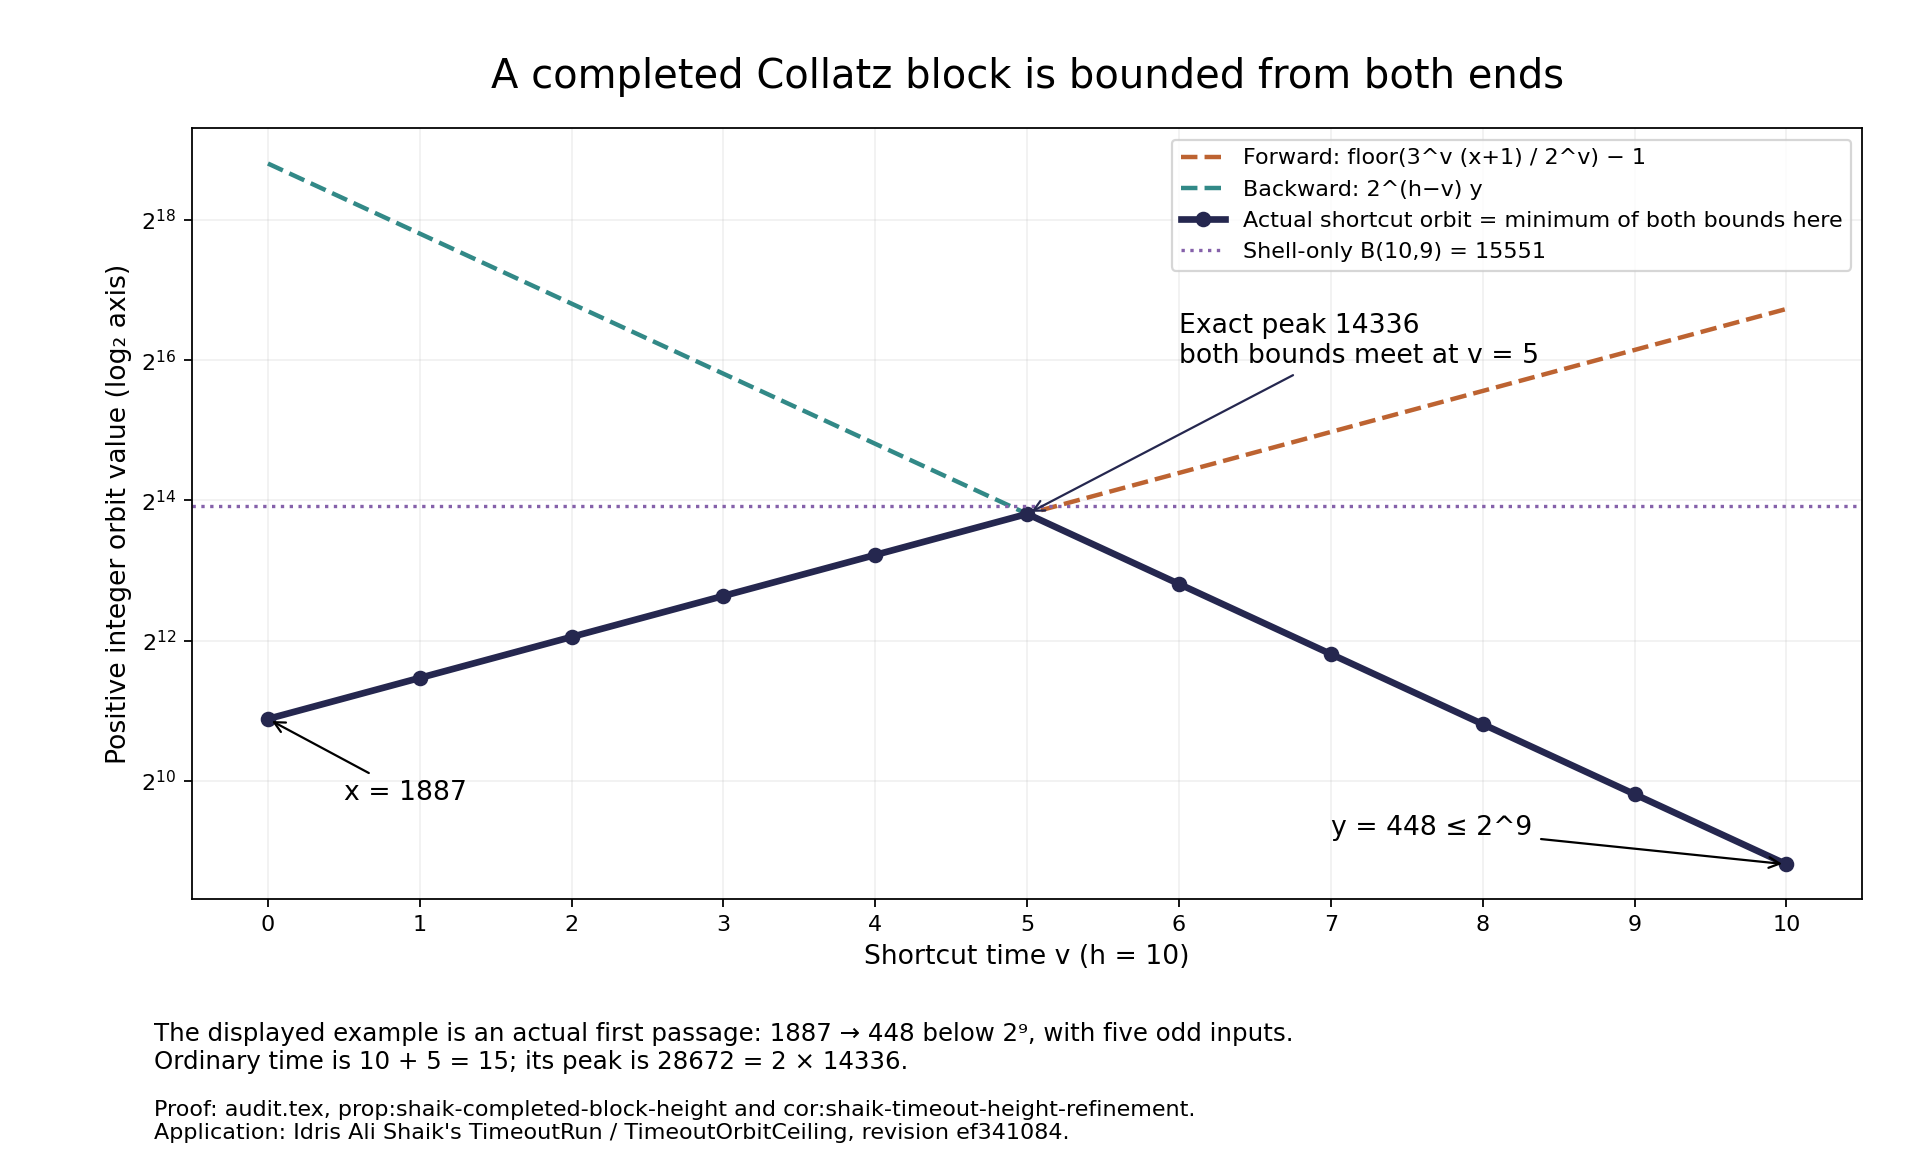
\includegraphics[width=\textwidth]{shaik_completed_height.png}}{%
\IfFileExists{../research_program/natural_density_audit_20260928/shaik_completed_height.png}{%
\includegraphics[width=\textwidth]{../research_program/natural_density_audit_20260928/shaik_completed_height.png}}{%
\IfFileExists{research_program/natural_density_audit_20260928/shaik_completed_height.png}{%
\includegraphics[width=\textwidth]{research_program/natural_density_audit_20260928/shaik_completed_height.png}}{}}}
\caption{Actual integer orbit and the two proved endpoint bounds, on a
logarithmic vertical axis. For this example their minimum is attained
at every displayed time. The dotted line is the larger bound using only
the source shell, target rank and deadline. Proof:
Proposition~\ref{prop:shaik-completed-block-height}. The timeout-block
application is to Shaik's construction \cite{Shaik2026v324}.
Source: \texttt{draw\_shaik\_completed\_height.py}.}
\end{figure}

\paragraph{Effect on the assembled statements.}
The map here is the identity on the original source integer and the
complete numerical run. Its endpoint, duration, odd-input count, first
passage and failure-envelope membership do not change. In
Corollary~\ref{cor:shaik-identical-endpoint-witness}, the timeout witness
therefore has this stronger finite height estimate on \emph{all} timeout-good
sources, not only on the all-prefix-good subset. All density estimates and
the exact partial-shell counts remain valid on the same sets.
Expansion to ordinary Collatz time keeps duration \(h+s_h(n)\) and the
same endpoint; it bounds ordinary intermediate values by twice
\eqref{eq:shaik-timeout-height-max}, because an inserted odd step is
\(3z+1=2T(z)\). That factor is retained, not absorbed without a margin.
The original asymptotic headline power ceiling is unchanged, but its
finite startup condition is weakened.

\paragraph{Attribution and verification.}
The original block types, endpoint decrease and high-stage height estimate
are Idris Ali Shaik's, revision \texttt{ef341084}:
\texttt{TimeoutRun.lean}, \texttt{TimeoutOrbitCeiling.lean},
\texttt{OrbitCeiling.lean}, and \texttt{TimeoutEndpointWitness.lean}
\cite{Shaik2026v324}. The elementary forward and backward inequalities
above are proved directly. No priority claim is made for them.
The improvement is their explicit two-sided use in these same source
blocks and its propagation without changing the retained set.
The universal statements here have written proofs; the accompanying
integer regressions do not certify the infinite analytic package.

\subsection{A kernel-checked certificate for the completed-block bounds}

\begin{proposition}[Discrete completed-height certificate]
\label{prop:shaik-completed-height-certificate}
The natural-number part of
Proposition~\ref{prop:shaik-completed-block-height} has a matching
twenty-nine-declaration Lean certificate. It proves
\eqref{eq:shaik-two-sided-block-height}, the exact shell maximum \(B(m,q)\),
the characterization of \(a\) as the greatest integer satisfying
\eqref{eq:shaik-height-crossing}, the two-candidate equality
\eqref{eq:shaik-height-two-candidates}, and monotonicity of \(B\) in both
shell and target ranks. In particular, a completed block with
\(x<2^{m+1}\), \(h\le m<S\), \(T^h(x)\le2^q\), and \(q<m\) satisfies
\[
 T^v(x)\le B(S-1,S-2)\qquad(0\le v\le h).
\]
The imported exact clock map gives the same endpoint at ordinary time
\(h+s_h(x)\), with every ordinary prefix bounded by \(2B(m,q)\).
All these statements quantify over their full natural-number domains;
they are not proofs by testing a bounded list of trajectories.
\end{proposition}
\begin{proof}[Proof and precise formal correspondence]
The module \texttt{CompletedHeight.lean} imports the independently pinned
\texttt{JointWitness} and \texttt{ClockAndRanks} modules. The imported
\texttt{shortcut}, \texttt{raw}, \texttt{iterate} and \texttt{oddCount}
are the same literal maps and recursive orbit used in the earlier
clock certificate. Induction on time identifies this recursion with
Shaik's \texttt{orbit\_zero} and \texttt{orbit\_succ}; no change of map
or time convention is made.

The declarations \texttt{forward\_scaled} and
\texttt{prefix\_backward} establish the two multiplied integer
inequalities. \texttt{prefix\_forward\_floor} uses natural division to
obtain exactly the displayed floor, and \texttt{two\_sided\_height}
takes the minimum. The definitions \texttt{forward}, \texttt{backward}
and \texttt{maxThrough} are respectively \(A_m(v)\), \(D_{m,q}(v)\)
and the inclusive maximum over \(0,\ldots,m\).
The shell theorem even needs only \(x<2^{m+1}\), not the shell's lower
bound; its specialization to the original shell is immediate.

The finite recursive search \texttt{lastGood} has a proved greatest-index
specification. \texttt{crossing\_integer\_iff} identifies its predicate
with the integer inequality in \eqref{eq:shaik-height-crossing}, retaining
the subtracted \(2^v\). The declarations \texttt{crossing\_greatest}
and \texttt{two\_candidate\_budget} prove the exact maximum and its
two-term evaluation, under \(1\le q<m\).
Finally, \texttt{budget\_mono} and \texttt{completed\_uniform\_height}
give the switch bound, and \texttt{completed\_raw\_height} and
\texttt{completed\_raw\_endpoint} apply the already certified ordinary
clock correspondence.

Lean 4.15.0 checked the saved module with pinned imports. Its reported
axiom sets are contained in \(\{\texttt{propext},\texttt{Quot.sound}\}\);
there are no admitted statements. Source, object, compiler, dependencies,
output, resource receipts and the three failed implementation attempts
are retained with hashes in \texttt{formal\_shaik\_height/}.
The successful single worker used \(184229888\) bytes at its measured
peak, below the watched \(2\) GiB tree cap.

The real-exponent inequality \eqref{eq:shaik-height-exponent}, the
source's high-window bound, concatenation through its complete timeout
run type, and the density estimates retain their written/source proofs.
They are not claimed as additional exports of this certificate.
Thus the certificate checks the exact discrete bounds consumed by
Corollary~\ref{cor:shaik-timeout-height-refinement}, not an entire analytic
package. The original run and high-stage mechanisms remain credited to
Idris Ali Shaik \cite{Shaik2026v324}.
\end{proof}

\subsection{Exact low-rank schedules and finite timeout clocks}
\label{subsec:shaik-low-schedule}
The leading timeout clocks were already obtained in
Corollary~\ref{cor:shaik-fixed-rate-clocks}. The remaining low-rank
reserve can be made considerably more precise at finite parameters.
This refinement uses Shaik's actual timeout run and terminal completion,
not the smaller all-prefix-good set:
\texttt{TimeoutRun.lean}, \texttt{TimeoutTimeSupport.lean},
\texttt{TimeoutFirstBad.lean}, and \texttt{TimeoutEndpointWitness.lean},
revision \texttt{ef341084} of \cite{Shaik2026v324}.
The source potential pays \(S^2\); \eqref{eq:shaik-low-triangle}
already replaced that by a triangular sum. The prescribed floor map
gives a still smaller, exactly computable reserve.

\begin{proposition}[Low continuation, with its dyadic branch]
\label{prop:shaik-low-schedule}
Fix integers \(2\le L<S\), \(K_0>0\), and
\(r_L=1-K_0/(2L)\in(0,1)\). Write
\[
 f(m)=\lfloor r_Lm\rfloor,\qquad Q(p)=f(p-1),
\]
and assume \(1\le Q(p)<p-1\) for \(L<p\le S\).
These are the literal target and admissibility conditions of the
timeout construction. Define finite sets of integers and integers
recursively, using strictly smaller arguments:
\begin{align}
 {\cal D}(p)&=\{0\},\quad F(p)=0 &&(p\le L), \notag\\
 {\cal D}(p)&=\{p-L\}\ \cup\
       \bigl([p-Q(p),p-1]_{\mathbb Z}+{\cal D}(Q(p))\bigr),
       &&(L<p\le S), \label{eq:shaik-low-duration-set}\\
 F(p)&=p-1+F(Q(p)) &&(L<p\le S). \notag
\end{align}
Here \(A+B=\{a+b:a\in A,\ b\in B\}\), not a disjoint union.
Start at a checkpoint \(x\in(2^{p-1},2^p]\), \(1\le p\le S\). Execute the original
low procedure, stopping upon a threshold at most \(L\), or completing
a dyadic checkpoint \(2^u\), \(u>L\), by \(u-L\) halvings.
For every successful continuation its total duration \(d\) satisfies
\[
 d\in{\cal D}(p),\qquad p-L\le d\le F(p)\quad(p>L).
\]
For \(L<p\le S\), moreover,
\begin{equation}\label{eq:shaik-low-budget}
 \begin{gathered}
 \min{\cal D}(p)=p-L,\quad\max{\cal D}(p)=F(p),\\
 F(p)\le\frac{p(p-1)-L(L-1)}2,\\
 F(p)<\frac{p-1}{1-r_L}=\frac{2L(p-1)}{K_0}.
 \end{gathered}
\end{equation}
The minimum and maximum are exact for the stated scalar construction.
Neither equality of \({\cal D}(p)\) with actual orbit durations nor
attainment of \(F(p)\) by an orbit is asserted.
\end{proposition}
\begin{proof}
For positive integers \(z\), \(T(z)\ge z/2\). Thus
\(T^h(x)\ge x/2^h\). At a non-dyadic checkpoint
\(2^{p-1}<x<2^p\), the parent is exactly \(p-1\).
If its passage to \(2^{Q(p)}\) succeeds, its deadline gives \(h\le p-1\),
whereas
\[
 2^{Q(p)}\ge T^h(x)\ge x/2^h>2^{p-1-h}
\]
forces the integer inequality \(h\ge p-Q(p)\).
Its landing is in \((2^{Q(p)-1},2^{Q(p)}]\).
At the dyadic checkpoint \(x=2^p\), the specified terminal completion
has exactly \(p-L\) steps. Induction proves the membership assertion.
It also explains why an upper endpoint is a separate branch, not
another non-dyadic parent of rank \(p-1\).

All the scalar intervals are nonempty, since \(Q(p)\ge1\).
Their recursive maximum is \(p-1+F(Q(p))\), which is at least
\(p-L\), since \(L\ge2\). If \(Q(p)>L\), their recursive minimum is
\(p-Q(p)+Q(p)-L=p-L\); if \(Q(p)\le L\), it is
\(p-Q(p)\ge p-L\). The dyadic branch attains the scalar minimum.
This proves both extrema, including the terminal overshoot.

For the upper bounds, put \(p_0=p\), \(p_{i+1}=Q(p_i)\) while
\(p_i>L\), and \(m_i=p_i-1\). The finite recursion gives
\(F(p)=\sum_{i:p_i>L}m_i\).
These are distinct decreasing integers in \([L,p-1]\), proving
the triangular bound. Successive nonterminal parents satisfy
\(m_{i+1}=\lfloor r_Lm_i\rfloor-1\le r_Lm_i\).
If there are \(t\ge1\) such parents, then
\[
 F(p)\le(p-1)\sum_{i=0}^{t-1}r_L^i
       <(p-1)/(1-r_L).
\]
The strict inequality uses \(0<r_L<1\) and finiteness of \(t\).
\end{proof}

\begin{proposition}[Only one low schedule can lead to a first timeout]
\label{prop:shaik-low-timeout-support}
Use Shaik's \(\mathrm{TimeoutHighRunData}\), with
\(M\ge S\) and \(p_{\rm Hi}.M_0\le L\), and the low hypotheses
of the preceding proposition.
Its non-dyadic high thresholds follow
\(m_0=M,\ q_i=\lfloor r_{\rm Hi}m_i\rfloor,\ m_{i+1}=q_i-1\).
Let \(p_0\le S\) be the first threshold entering the low region,
and suppose \(p_0>L\). Let \([a,b]_{\mathbb Z}\) be any proved
integer interval containing its high arrival times, with \(a\le b\).
For example, at each high block use
\[
 a_i=\max\!\left(1,\left\lceil
          \frac{(1-t_i)m_i-q_i}{g}\right\rceil\right),\qquad
 b_i=\min\!\left(m_i,\left\lceil
          \frac{(1+t_i)(m_i+1)-q_i+1}{g}\right\rceil-1\right),
\]
and \(a=\sum a_i,\ b=\sum b_i\); this retains the closed lower
and strict upper endpoints of \eqref{eq:shaik-one-sided-corridor}.
An empty block interval means that no such high continuation exists.

Continue \(p_{j+1}=Q(p_j)\) until the first \(p_t\le L\).
Only \(p_0,\ldots,p_{t-1}\) can support the source's low first-timeout
sets. For \(0\le j<t\) put
\[
 V_j=\sum_{i<j}(p_i-1),\qquad
 I_j=[a+p_0-p_j,\ b+V_j]_{\mathbb Z},\qquad
 W_j=b-a+1+\sum_{i<j}(p_{i+1}-1).
\]
Every arrival time in \(\mathrm{timeoutFirstBadSourcesAtRank}\)
at \(p_j\) belongs to \(I_j\), and \(\#I_j=W_j\).
The other low first-timeout sets, for \(L<p\le S\), are empty.
This is not an assertion that the source's larger
\(\mathrm{timeoutFeasibleTimes}\) is empty off that list.

Fix a rational \(0<r_*\le\min(r_{\rm Hi},r_L)\). Retain the
rankwise reverse-transport hypotheses
\(p_j<M\) and \((p_j+2)/(r_*2^{p_j})\le1/3\).
Writing \({\cal B}_{p}=\mathrm{timeoutLandingBad}(K_0,L,p)\), one obtains
the finite union estimate
\begin{equation}\label{eq:shaik-low-refined-count}
 \frac{\#\bigcup_{L<p\le S}\mathrm{timeoutFirstBadSourcesAtRank}(p)}
      {2^M}
 \le
 \sum_{j<t}W_j
       \left(2^{p_j-M}+\frac{3(p_j+2)}{r_*}\right)
       \frac{\#{\cal B}_{p_j}}{2^{p_j}} .
\end{equation}
Each \(W_j\) may also be replaced by its minimum with any previously
proved cardinality bound for the source's feasible-time set at \(p_j\).
\end{proposition}
\begin{proof}
In a run ending at an actual timeout, no previous checkpoint was
dyadic. Indeed, from \(2^u\) every subsequent positive-threshold
first passage is an exact halving passage, remains dyadic, and
cannot time out. At a final putative timeout rank \(p>L\), the
target \(Q(p)\ge1\) is reached from \(2^p\) in
\(p-Q(p)\le p-1\) steps, directly contradicting that timeout.
No such history can leave the low region: reached thresholds
strictly decrease, and the high constructor requires parent
\(m\ge S\) with previous threshold \(m+1\).

Consequently every high continuation in a first-timeout history has
parent \(q_i-1\), and every low continuation has parent \(p_i-1\).
The floor maps fix both lists. This reasoning applies to all the
source's inductive records, including ones which were not explicitly
stopped at an earlier terminal rank: strict decrease prevents their
return to \(p>L\). It proves the asserted empty first-timeout sets,
without removing any source from the literal envelope.

Before the timeout at \(p_j\), every low block succeeds, so its
duration \(d_i\) is in \([p_i-p_{i+1},p_i-1]_{\mathbb Z}\).
The sum of these independent scalar intervals is exactly
\([p_0-p_j,V_j]_{\mathbb Z}\). To prove this last equality
constructively, start every coordinate at its lower endpoint.
For a requested excess \(e\) between zero and the sum of the
widths, add the lesser of \(e\) and the first width to the first
coordinate, subtract that addition from \(e\), and repeat.
The remaining excess is zero after the last coordinate.
This is a section of the sum map on scalar tuples, not a procedure
for constructing a Collatz orbit. Applying it also to \([a,b]\)
gives the exact scalar interval \(I_j\). Its cardinality is
\[
 b+V_j-(a+p_0-p_j)+1
 =b-a+1+\sum_{i<j}(p_{i+1}-1)=W_j.
\]

Restrict the source transport to the intersection of \(I_j\) with
its original feasible times. The original source, landing, direct
first passage and reverse-loss bound are unchanged. Apply
\texttt{timeoutFirstBadSourcesAtRank\_card\_le}'s underlying
finite-time transport estimate to this smaller support. In fact its
unabsorbed version,
\texttt{lossFiltered\_arbitraryTarget\_transport\_atTimes}
in \texttt{TimeSupportTransport.lean}, gives the exact factor
\((1+3(p_j+2)2^{M-p_j}/r_*)\#{\cal B}_{p_j}\).
Counting the restricted times by \(W_j\), or by the stated minimum,
dividing by \(2^M\), and summing proves
\eqref{eq:shaik-low-refined-count}. Since \(p_j<M\), replacing
\(2^{p_j-M}\) by \(1\) recovers the source's uniform factor
\((1+3(p_j+2)/r_*)\#{\cal B}_{p_j}/2^{p_j}\).
The unabsorbed expression retains the smaller finite boundary term.
Overlaps only make the union smaller; no disjointness assumption is needed.
\end{proof}

\begin{corollary}[Finite clocks and height on the unchanged successful paths]
\label{cor:shaik-low-schedule-clocks}
In the preceding setting every timeout-good path which enters
the low phase has its original completed witness \(y\le2^L\) by
integer shortcut time
\[
 k\le K:=b+F(p_0).
\]
No separate additional \(S\)-step halving reserve is needed:
the dyadic terminal branch is already included in \(F\).
For \(n\in I_M\) on this successful set, define
\begin{equation}\label{eq:shaik-low-integer-clock}
 J(K,M,L)=\max\{s\in[0,K]_{\mathbb Z}:3^s2^M\le2^{K+L}\}.
\end{equation}
The set is nonempty whenever such a witness exists.
The same path has at most \(J(K,M,L)\) odd inputs and at most
\(K+J(K,M,L)\) ordinary Collatz steps to \(y\).
For odd \(n\), completing the terminal even tail and cutting at odd
states gives at most \(J(K,M,L)\) Syracuse returns.
Its shortcut height is at most
\[
 H(n)=\max\{n^{1+\tau}, B(S-1,S-2)\},
\]
and its ordinary height is at most \(2H(n)\).
The explicit density multiplier in \eqref{eq:shaik-low-refined-count}
and these clocks therefore apply without a change of accepted sources.
\end{corollary}
\begin{proof}
Apply Proposition~\ref{prop:shaik-low-schedule} at the actual high
landing, allowing its dyadic branch. The high time is at most \(b\).
If \(s\) is the odd-input count, the exact affine iterate identity gives
\(3^sn\le2^ky\). Hence
\(3^s2^M\le2^{k+L}\le2^{K+L}\) and \(s\le k\le K\).
This both proves nonemptiness in \eqref{eq:shaik-low-integer-clock}
and bounds \(s\). Expansion and cutting are the exact path maps
of Proposition~\ref{prop:shaik-core-certificate}; expansion takes
\(k+s\) ordinary steps. The height is
Corollary~\ref{cor:shaik-timeout-height-refinement}, including its
factor two for the inserted ordinary odd edges. The final even
tail only decreases values.
\end{proof}

\paragraph{The maps and their information loss.}
An actual path is sent to its high prefix, decreasing low ranks,
block durations and terminal branch. Its scalar duration record
forgets intermediate values and parity, so it has no asserted
inverse to an orbit. On independent scalar duration tuples, the
sum map has the explicit section in the proof above; its fibres
are exactly the tuples in their respective intervals with the
same sum. Decorating the actual path with its new budget changes
neither the path nor its accepted source and has the identity
inverse after forgetting that decoration. This is the comparison
needed for the original failure-envelope and witness statements.

\begin{figure}[ht]
\centering
\fbox{\begin{minipage}{0.92\linewidth}
Take \(L=5,\ K_0=4,\ r_L=3/5,\ p=6\); thus \(Q(6)=3\).
\[
\begin{array}{c|c|c}
 \text{branch at }(2^5,2^6]&\text{duration}&\text{terminal value}\\ \hline
 x=64&6-5=1&32\\
 32<x<64&h\in[6-3,5]_{\mathbb Z}&T^h(x)\le8
\end{array}
\]
The scalar set is \({\cal D}(6)=\{1,3,4,5\}\), not \([1,5]_{\mathbb Z}\).
An actual successful interior example is
\(37\mapsto56\mapsto28\mapsto14\mapsto7\), of duration \(4\).
The scalar set contains \(5\), but this figure does not claim an
orbit realizes every scalar possibility.
\end{minipage}}
\caption{The upper-endpoint completion and the interior first passage
are distinct branches of the same timeout procedure. The strict lower
landing boundary produces the lower duration \(p-Q(p)\).
Complete proof: Proposition~\ref{prop:shaik-low-schedule}.
The underlying run and terminal completion are Shaik's
\cite{Shaik2026v324}; exact integer checks and reproducible figure source
are recorded in \texttt{check\_shaik\_low\_schedule.py} and
\texttt{draw\_shaik\_low\_schedule.py}.}
\end{figure}

For a concrete finite comparison, take \(L=20,\ K_0=4,\ p_0=S=64\).
Then \(r_L=9/10\), and the low threshold list is
\[
 64,\ 56,\ 49,\ 43,\ 37,\ 32,\ 27,\ 23,\ 19.
\]
The exact scalar reserve is
\(F(64)=63+55+48+42+36+31+26+22=323\).
The triangular reserve in \eqref{eq:shaik-low-triangle} is \(1826\);
the source's \(S^2\) potential reserve is \(4096\).
These are bounds on the low part, not on the preceding high clock.

\paragraph{What has and has not changed.}
The new recursion and directed supports refine finite reserves in the
existing timeout proofs. They do not change the leading clock constants
already proved above, and no new asymptotic density exponent follows
merely from this refinement. At a logarithmic switch the triangular
bound still gives \(F(p_0)=O(\log^2 M)\), below the existing
square-root clock error. The gain is an exact, usable finite budget,
including its floor schedule, possible duration gaps, and smaller
rankwise transport multiplier. The stronger original parameter bundle
is not modified; the finite result uses only the displayed stage and
transport hypotheses. These are complete written proofs with finite
regressions, not new Lean exports or a replay of the whole analytic
dependency closure.

\subsection{Joining the drift prefix to the timed almost-bounded path}
\label{subsec:shaik-allikvere-splice}

The high-rank construction and the timed fixed-target theorem describe
the same deterministic orbit, but supply different information about it.
The former controls its height and the time already spent; the latter
bounds its total number of odd returns. Subtracting these times leaves
only a sublinear number of returns after a polylogarithmic landing.
This removes the extra \(\log_2 n\) in the crude raw-clock conversion.

Here \(d=\log(4/3)\), \(g=1-\tfrac12\log_2 3\), so \(2g\log2=d\).
The analytic inputs are the uniform timed count reconstructed from
Allikvere's version--2 argument
(\href{https://doi.org/10.5281/zenodo.21499244}{author source},
section ``A time budget and an explicit rate'', labels
\texttt{prop:timed}, \texttt{thm:quant}) and Tao's first-passage method, and Shaik's
high-certificate transport \cite{Shaik2026v324}, reconstructed above.
Precisely, the timed input used here is
\[
 \#\{n\le X:n\ {\rm odd},\
       \nexists k\le K(n):\Syr^k(n)\le B\}
 \le C_c X(\log B)^{-c},
\]
\[
 K(n)=d^{-1}\log n+C_K(\log(n+2))^{4/5},
\]
for all \(X,B\ge2\), \(B\) integral, \(0<c<1/17.232\).
The absolute \(C_K\) is independent of \(B,c\).
This is the proved timed fixed-target count earlier in this manuscript,
including its stronger kernel exponent and exact power-interval cover,
not an additional hypothesis about landing distributions.

\begin{lemma}[The high prefix has two-sided clocks]
\label{lem:shaik-high-two-sided}
For any \(\eta,e>0\), there are constants \(A,C,M_0\), a
deterministic integer \(p_M=O_{\eta,e}(\log(M+2))\), and sets
\(G_M\subseteq I_M\), for \(M\ge M_0\), such that
\[
 \#(I_M\setminus G_M)\le C2^M M^{-e},\qquad
 Y_M:=2^{p_M}\gg_{\eta,e}(M+2)^2.
\]
Each \(n\in G_M\) has a first shortcut passage to \(Y_M\) of
length \(H\), landing \(y\in(Y_M/2,Y_M]\), and odd-step count \(s\).
With \(E_M=\sqrt{M\log(M+2)}\), these satisfy
\begin{equation}\label{eq:shaik-high-three-clocks}
 H=M/g+O_{\eta,e}(E_M),\quad
 s=M/(2g)+O_{\eta,e}(E_M),\quad
 H+s=3M/(2g)+O_{\eta,e}(E_M).
\end{equation}
The shortcut prefix stays below \(n^{1+\eta}\).
For odd \(n\), appending the even tail of \(y\) ends at
\(z=\operatorname{oddpart}(y)=\Syr^s(n)\le Y_M\), with at most
\(p_M\) additional halvings and no additional odd step.
Moreover, \(s\) is the first Syracuse passage time to \(Y_M\).
The expanded ordinary prefix stays below \(2n^{1+\eta}\).
\end{lemma}
\begin{proof}
Choose \(a_0<r<1\), \(0<\tau<\min(r-a_0,\eta,1)\), then \(D\)
and \(C_{\rm sw}\) so that
\[
 D/\sqrt{C_{\rm sw}}\le\tau,\quad
 \min(c_0D^2,C_{\rm sw}\log2)>e+2,\quad
 rC_{\rm sw}\log2>2.
\]
Set \(S=\lceil C_{\rm sw}\log(M+2)\rceil\). Use only the high
phase of Theorem~\ref{thm:shaik-shell-drift}: reject the initial
failed certificate and the first failed high certificate or upper
endpoint at threshold rank greater than \(S\). Stop at the first
threshold rank at most \(S\), including its upper endpoint.
No low certificate, timeout or low-density estimate is used.

Before this stop the ranks are exactly
\(m_0=M,\ q_i=\lfloor rm_i\rfloor,\ m_{i+1}=q_i-1\).
The final threshold \(p_M=q_j\) is therefore independent of \(n\)
and satisfies \(\lfloor rS\rfloor\le p_M\le S\).
The high-failure calculation \eqref{eq:shaik-high-refined} gives
\(O(2^M M^{-e})\) discarded sources. In detail the normalized
charge is \(O((1+ME_M)M^{-\phi})\), where
\(\phi=\min(c_0D^2,C_{\rm sw}\log2)>e+2\); this is \(O(M^{-e})\).
Since \(2^{\lfloor rS\rfloor}\ge (M+2)^{rC_{\rm sw}\log2}/2\),
the asserted lower bound on \(Y_M\) follows.

The two sides of \eqref{eq:shaik-one-sided-corridor}, with
\(p_M=O(\log M)\), \(j=O(\log M)\), and
\(\sum_i t_{m_i}m_i=O(E_M)\), give \(gH=M+O(E_M)\).
Each earlier segment stays above its own target, which is greater
than \(Y_M\); hence their concatenation is the direct first passage
to \(Y_M\). Proposition~\ref{prop:shaik-defect} gives
\[
 n=2^HyP/3^s,\qquad 0\le1-P<H/(3Y_M).
\]
Thus \(P\ge1/2\) for large \(M\). Since
\(M\le\log_2n<M+1\) and \(p_M-1<\log_2y\le p_M\),
\[
 (\log_2 3)s=H+\log_2(y/n)+\log_2P
            =H-M+O(\log(M+2)).
\]
Using \(1-g=\tfrac12\log_2 3\) proves all three clocks.
The decreasing high checkpoints and their \(W_{t_m}\) bounds give
the stated shortcut height. Expanding an odd shortcut edge inserts
the height \(3x+1\), twice its following shortcut value, and inserts
one extra ordinary step. This proves the ordinary height and clock.

For odd \(n\), cutting the expanded path at odd states and appending
the terminal halvings gives the first \(s\) actual Syracuse returns.
Every earlier odd state is before the shortcut crossing and exceeds
\(Y_M\). The appended tail only decreases and has length
\(v_2(y)\le p_M\). This proves the first-passage assertion, including
the case that \(y=Y_M\) and its odd part is \(1\).
\end{proof}

\begin{lemma}[Exact same-orbit continuation]
\label{lem:shaik-same-orbit-tail}
Let \(n\) be odd and let \(s\) be its finite first Syracuse
passage to \(Y\ge1\), with \(z=\Syr^s(n)\le Y\).
Suppose its first Syracuse hit of the integer target \(B\ge1\)
has time \(\sigma\le K\).
If \(B\ge Y\), then \(\sigma\le s\). If \(B<Y\), then
\(s\le\sigma\), and the remaining \(r=\sigma-s\) returns satisfy
\begin{equation}\label{eq:shaik-exact-tail}
 0\le r\le K-s,\qquad
 \ell_C\le3r+\log_2 z,\qquad
 \ell_T\le2r+\log_2 z,\qquad
 \max({\rm ordinary\ tail})\le2^{r+1}Y.
\end{equation}
Here \(\ell_C,\ell_T\) are the actual ordinary and shortcut lengths
from \(z\) to \(\Syr^\sigma(n)\); the estimates include \(r=0\).
\end{lemma}
\begin{proof}
Before \(s\), every odd state exceeds \(Y\). The two orderings of
first passages follow immediately, including equality.
For \(z_i=\Syr^i(z)\), put
\(a_i=v_2(3z_i+1)\ge1\), \(v=\sum_{i<r}a_i\).
Exact concatenation gives \(\ell_C=r+v\), \(\ell_T=v\), and
\[
 2^v z_r=z\prod_{i<r}(3+1/z_i)\le4^rz.
\]
Since \(z_r\ge1\), \(v\le2r+\log_2z\).
Also \(z_i\le2^iz\), because \(\Syr(x)\le2x\).
Every inserted ordinary odd peak is at most
\(4z_i\le2^{i+2}Y\); for \(i<r\) this is at most \(2^{r+1}Y\).
The intervening halvings decrease. The empty tail has height \(z\le Y\).

This construction is a map from two marked prefixes of the same
orbit to their common first-\(B\) prefix. On \(B<Y\) it concatenates
the retained first-\(Y\) prefix and the actual tail of length
\(\sigma-s\); on \(B\ge Y\) it truncates the retained prefix.
It neither chooses a new source at \(z\) nor transports a probability
law to \(z\). Retaining \(n,s,\sigma\) determines all these states;
forgetting the unused suffix is not an invertible map on arbitrary
path records.
\end{proof}

\begin{theorem}[Drift clocks and height for almost-bounded targets]
\label{thm:shaik-allikvere-drift-target}
For every \(\beta,e>0\) there is \(A_{\beta,e}>0\) such that,
putting
\[
 R_j(n)=\frac{j}{d}\log n+
             A_{\beta,e}(\log(n+2))^{4/5},\qquad j=1,2,3,
\]
the following holds. For every \(X\ge2\), integer \(B\ge2\), and
\(0<c<1/17.232\), all but at most
\begin{equation}\label{eq:shaik-allikvere-count}
 C_c X(\log B)^{-c}
       +C_{\beta,e}X(\log(X+2))^{-e}
\end{equation}
positive integers \(n\le X\) have one actual orbit prefix ending at
an odd integer at most \(B\). Its shortcut length is at most \(R_2(n)\),
its ordinary length at most \(R_3(n)\), and its ordinary height
(including its initial state) at most \(n^{1+\beta}\).
It contains at most \(R_1(n)\) odd steps; for odd \(n\) this is
its Syracuse return count.
The constants \(A_{\beta,e},C_{\beta,e}\) do not depend on \(B,c,X\).
Consequently, for every \(f(n)\to+\infty\), the same three clocks
and height reach a value strictly below \(f(n)\) for a set of
natural density one. The clocks do not depend on \(f\).
\end{theorem}
\begin{proof}
First restrict to odd \(n\). Take the high-prefix lemma with
\(0<\eta<\beta\), and intersect its good set with the successful
set of the timed fixed-target count. Their complements are counted
on the original integers \(n\), so the union bound is legitimate
without independence or a landing-distribution assumption.
For \(n\in I_M\) outside this union, write \(\sigma\le K(n)\)
for the first odd hit of \(B\), and \(s,z,Y_M\) for the high passage.

If \(B\ge Y_M\), the desired prefix is a truncation of the high
prefix completed to its odd landing. Its clocks and height already
have the asserted bounds, since
\(E_M=o((\log(n+2))^{4/5})\).
If \(B<Y_M\), the two-sided odd clock gives
\[
 0\le r=\sigma-s\le
 C_K(\log(n+2))^{4/5}+O_{\beta,e}(E_M)
       =O_{\beta,e}((\log(n+2))^{4/5}).
\]
Here \(s=d^{-1}\log n+O_{\beta,e}(E_M)\), not just an upper bound.
The preceding lemma bounds the remaining ordinary and shortcut
lengths by \(O_{\beta,e}((\log(n+2))^{4/5})\), because
\(\log_2z\le p_M=O_{\beta,e}(\log\log(n+2))\).
Adding them to \eqref{eq:shaik-high-three-clocks}, including the
at most \(p_M\) terminal halvings, proves the three clocks.
The high ordinary height is \(2n^{1+\eta}\le n^{1+\beta}\) for
large \(n\), while the tail height satisfies
\[
 \log(2^{r+1}Y_M)
      =O_{\beta,e}((\log(n+2))^{4/5})=o(\log n).
\]
It is therefore at most \(n\) for large \(n\), uniformly in \(B\).
Finite startup inputs can be put in the high exceptional set.

The dyadic shell count for the high exceptions is
\(O_{\beta,e}(X(\log(X+2))^{-e})\): split shells at
\(\tfrac12\log_2X\), bound the lower part by \(O(\sqrt X)\),
and sum the upper bounds geometrically. The timed exceptions have
the first term of \eqref{eq:shaik-allikvere-count}.
This proves that estimate for odd sources.

For general \(n=2^a u\), \(u\) odd, prepend its \(a\) halvings.
Since \(j\log2/d>1\) for \(j=2,3\),
\[
 a+(j/d)\log u\le(j/d)\log n,\qquad
 \log(u+2)\le\log(n+2).
\]
The odd-step count acquires no term \(a\), and the height becomes
at most \(\max(n,u^{1+\beta})\le n^{1+\beta}\).
The exact fibres \(u\mapsto2^au\) give the sum of odd exception
counts at cutoffs \(X/2^a\).
The target-dependent terms sum to at most
\(2C_cX(\log B)^{-c}\). For the high terms with \(X/2^a\ge\sqrt X\)
use \(\log(X/2^a+2)\ge\tfrac12\log X\); the remaining cutoffs
contribute at most \(\sum_{X/2^a<\sqrt X}X/2^a\le2\sqrt X\).
Absorb these and bounded \(X\) into \(C_{\beta,e}\), and the factor
two into \(C_c\). No equality of odd and all-integer densities is used.

Finally set \(b(X)=\inf_{n\ge\sqrt X}f(n)\) and
\(B(X)=\lceil b(X)\rceil-1\). Eventually \(B(X)\ge2\),
\(B(X)\to\infty\), and \(B(X)<f(n)\) for \(n\ge\sqrt X\).
The at most \(\sqrt X\) smaller inputs, together with
\eqref{eq:shaik-allikvere-count}, have total proportion tending to
zero. All constants were selected before \(B\) or \(f\).
\end{proof}

\paragraph{Relation to the literature and the earlier clocks.}
The coefficient \(3/d\) is the ordinary drift coefficient, not a new
prediction. Inselmann's \cite[Theorems 1.9--1.10]{Inselmann2024v3}
trajectory results already give ordinary and Syracuse power envelopes
through times \(3d^{-1}\log n\) and \(d^{-1}\log n\), respectively,
on natural-density-one sets. His shortcut theorem uses
\(2d^{-1}\log n\). Those statements have fixed power tolerances
\(n^{\pm\epsilon}\). The proof above instead retains the explicit
\(O((\log n)^{4/5})\) clock error and joins the high prefix to the
arbitrary-diverging-target conclusion, with the displayed quantitative
fixed-target exception count and one common height-controlled path.
It uses the written analytic reconstructions; it is not a Lean
certification of either complete source package or a priority claim.

Allikvere's original valuation telescope gives
\((3/d+1/\log2)\log n+O((\log n)^{4/5})\).
That remains a valid bound. The improvement here is a different
use of its timed witness, not a correction to that telescope or to
Tao's theorem. Mazur's logarithmic-time theorem can be joined at the
same first passage, but its inspected leading odd-clock constant
is larger than \(1/d\). Subtracting \(s\) from that estimate leaves
an \(O(\log n)\) remainder, so this particular substitution does not
give the subpower tail-height estimate just proved. This says what
the displayed bounds imply; it does not assert different actual
orbits or the impossibility of a sharper Mazur clock.

\begin{figure}[ht]
\centering
\fbox{\begin{minipage}{0.92\linewidth}
\[
\begin{aligned}
 n&\xrightarrow[\text{height }\le2n^{1+\eta}]
 {\ s=d^{-1}\log n+O(\sqrt{\log n\log\log n})\ } z\le Y_M,\\[1.5ex]
 z&\xrightarrow[\text{height }\le2^{r+1}Y_M]
 {\ r\le K(n)-s=O((\log n)^{4/5})\ }\Syr^\sigma(n)\le B.
\end{aligned}
\]
This is the case \(B<Y_M\). For \(B\ge Y_M\), truncate the first
arrow at its first odd hit of \(B\). The same initial integer labels
both arrows; no new sampling occurs at \(z\).
\end{minipage}}
\caption{Joining two clocks on one orbit. The high-prefix construction
is Shaik's; the total odd clock comes from the reconstructed
Allikvere--Tao argument. Subtracting a lower prefix bound from an upper
total bound controls the actual remaining path. Proofs:
Lemmas~\ref{lem:shaik-high-two-sided},
\ref{lem:shaik-same-orbit-tail} and
Theorem~\ref{thm:shaik-allikvere-drift-target}.
The diagram is schematic, not a numerical trajectory.}
\end{figure}

\section{What has been checked at this stage}
Theorem~\ref{thm:shaik-allikvere-drift-target} joins the reconstructed
timed count and high-prefix transport on the same orbit. It proves
the three drift clocks with an explicit sublinear remainder, the
ordinary height bound and the uniform fixed-target exception count.
Its complete argument is written above; the finite path regressions
do not certify the analytic inputs, and it is not a new Lean export.
Proposition~\ref{prop:shaik-low-schedule} and
Proposition~\ref{prop:shaik-low-timeout-support} give exact low-rank
duration sets and first-timeout supports; Corollary~\ref{cor:shaik-low-schedule-clocks}
propagates these into finite three-clock and height bounds on unchanged paths.
These new general written proofs are not Lean exports.
Proposition~\ref{prop:shaik-completed-block-height} and
Corollary~\ref{cor:shaik-timeout-height-refinement} give written two-sided
height bounds on the unchanged timeout-good set. Their discrete completed-block
bounds now have the matching certificate in
Proposition~\ref{prop:shaik-completed-height-certificate}; the real exponents,
high-stage bounds and whole-run analytic assembly remain written/source results.
Proposition~\ref{prop:shaik-timeout-forgetting} gives a written exact
comparison of the original failure envelopes and numerical run records;
Corollary~\ref{cor:shaik-identical-endpoint-witness} identifies the literal
witness predicates and propagates the count bounds. This comparison has
not been independently compiled as a source-package Lean theorem.
Proposition~\ref{prop:shaik-dyadic-certificate} has a matching
twenty-three-declaration Lean certificate for the discrete count and
ordinary-clock consumer. Its scope is separate from the real analytic
endpoint theorem and the full source dependency closure.
Theorem~\ref{thm:shaik-refined-moving-endpoint} assembles the refined
all-prefix parameter domain, explicit constants, original failure envelope,
same-witness clock and height, and exact arbitrary-prefix count.
Corollary~\ref{cor:shaik-refined-moving-clocks} transports its actual paths
to the other two clocks. These analytic statements have written proofs,
not new Lean certificates.
Proposition~\ref{prop:shaik-moving-reachable-support} proves the exact
rank restriction and time enclosure; Corollary~\ref{cor:shaik-moving-linear-high}
propagates it to the unchanged moving envelope. These are written proofs.

Proposition~\ref{prop:shaik-least-moving-startup} gives the least possible
startup and an explicit subthreshold repair, with the finite threshold
\eqref{eq:shaik-finite-moving-threshold}. These remain written proofs.

Proposition~\ref{prop:shaik-exact-moving-startup} proves the necessary
and sufficient closed startup threshold for the original scalar interface,
and \eqref{eq:shaik-common-moving-startup} propagates it into the low profile.
These are written proofs, not further Lean exports.

Proposition~\ref{prop:shaik-reflection-certificate} has a new independently
compiled 31-statement finite Lean certificate, including literal counting
semantics. Proposition~\ref{prop:shaik-moving-low-reserve} and its subsequent
profile calculation are complete written analytic refinements, not Lean
exports of the real-variable estimates.

The uniform square-root estimate and its exact reflection map are proved in
Proposition~\ref{prop:shaik-uniform-prefactor} and
Lemma~\ref{lem:shaik-exact-reflection}. Corollaries~\ref{cor:shaik-prefactor-propagation}
and~\ref{cor:shaik-shrinking-prefactor} propagate it through the existing
fixed and shrinking constructions. These are written analytic proofs,
not new Lean exports.

Proposition~\ref{prop:shaik-full-entropy} retains the full fixed-tolerance
entropy rate by an explicit rank-dependent auxiliary barrier.
Corollary~\ref{cor:shaik-entropy-propagation} carries it through the
original pullbacks and fixed-barrier descent, without altering their
sets or clocks. These real-variable results have written proofs,
not new Lean exports.

Proposition~\ref{prop:shaik-clipped-horizon} and
Corollary~\ref{cor:shaik-closed-graded} retain the actual stopping map,
remove the extra graded-clock startup payment, and admit the closed
fixed-depth exponent with one simultaneous exceptional-count estimate.
These are complete written proofs; no new analytic Lean export is claimed.

The sharp shifted-shell assembly, its integer linear boundary, and the
unclipped same-schedule application are proved in
Propositions~\ref{prop:shaik-sharp-shell}--\ref{prop:shaik-linear-shell}
and Corollary~\ref{cor:shaik-unclipped-source-count}.
Their analytic bounds are written proofs, not new Lean exports.

Proposition~\ref{prop:shaik-joint-certificate} now has a separate
nine-statement Lean certificate for its exact integer witness/count
mechanism. Proposition~\ref{prop:shaik-matched-schedule} is a complete
written endpoint calculation for the explicitly shifted source schedule;
its real-variable estimates are not included in that certificate.

Proposition~\ref{prop:shaik-log-pullback} retains the endpoint exponent
on the original fixed-depth bootstrap sets, with its logarithmic factor
and explicit prefactor recurrence. Proposition~\ref{prop:shaik-absorbing-startup}
uses their absorbing startup branch to remove the coarse intermediate
target and clock losses. These are written deductions from the source
transport and deterministic dynamics, not new Lean exports.

Proposition~\ref{prop:shaik-stretched-fixed} reconstructs the full
stretched-logarithmic exceptional power, with the same target, clock
and height witness. Proposition~\ref{prop:shaik-graded-quantitative}
retains an explicit power-saving count for the graded fixed-power
clock and carries the witness through all three clocks.
The source already contains a positive power-saving antecedent for
its graded theorem. These written deductions are not new Lean exports.

Corollary~\ref{cor:shaik-critical-rates} retains the two boundary
iterated-logarithmic exceptional powers of Shaik's critical schedules.
Proposition~\ref{prop:shaik-slow-factor} reconstructs the arbitrary
diverging final factor and preserves its shifted quantitative profile.
Both use the exact ceiling and the literal simultaneous-witness set.
Their real-variable proofs are written, not newly kernel checked.

Proposition~\ref{prop:shaik-prescribed-rate} constructs every prescribed
strict rate in Shaik's first fixed-target corollary, including explicit
stage startups. Its proof follows the exact rate through the source
package to the same-witness global exceptional count. This is written
source-level reconstruction, not an additional Lean certificate.

Proposition~\ref{prop:shaik-parity-decoder} adds an executable inverse,
exact integer fibres and an independently checked binary-shift identity.
Corollary~\ref{cor:shaik-parity-counting} gives the full written
counting and conditioned-image comparison. Proposition~\ref{prop:shaik-weighted-count}
now adds general Lean proofs of weighted reindexing and the complete-shell
binomial count. Proposition~\ref{prop:shaik-startup-rate} retains every
incoming logarithmic exceptional exponent under a finite startup change;
its exact finite-count inequality is also checked by Lean, while its
real-variable absorption argument is given in full above.

Proposition~\ref{prop:shaik-core-certificate} now has a scoped,
independently compiled Lean certificate for its exact integer and path
statements. The complete analytic density argument is not thereby formalized.

Section~\ref{sec:shaik-timeout} now reconstructs the uniform prefix
bound, integer timeout tail, deterministic time supports and full critical
shell estimate. It retains the endpoint rate and proves additive-error
shortcut, raw and odd-return clocks. This is a written reconstruction,
not a replay of the complete Lean dependency closure.

Section~\ref{sec:shaik-reverse} reconstructs selected deterministic
proofs in Shaik's manuscript and pinned Lean source, with exact product
defects, smaller loss and fibre constants, and a proved passage-clock
correspondence. Its full argument is also in cumulative chapter 01n.
The rational checks cover actual finite paths and exact interval counts;
they do not verify the whole natural-density package or its formal build.


Section~\ref{sec:mazur-genuine-assembly} completes the four comparisons
for actual first passage, the exact whole-source mixtures and the
nonpassage completion. Its four written results retain all original
band normalizers, targets and boundary terms; the independent finite
regressions are in \texttt{check\_mazur\_genuine.py}.
Section~\ref{sec:mazur-real-timed} now gives the exact totalizer loss,
real-source comparison, time-carrying recurrence and fixed-target
timed density estimates, with their complete written proofs.
The finite checks in \texttt{check\_mazur\_real\_timed.py} test the
algebra and path implications; they do not certify infinite claims.
No Lean replay is claimed.

Section~\ref{sec:mazur-exterior-assembly} now reconstructs the original
weighted endpoint fibres, sums the terminal factor inside the two
one-sided tail estimates, and completes both full reference profiles.
The total coefficient is bounded by $2+3B^{-4997/600000}$; the
exterior majorant is $(4+o_C(1))N^{-64C^2/(\log2)^3}$.
The exact finite kernel estimate retains its original mass, signed
denominator corrections and separate interior/exterior charges.
The genuine-passage assembly is now proved above; the next source work
is the original clock/iteration consumers and connected Shaik comparison.
Exact finite regressions do not certify
the asymptotic estimates or constitute a Lean replay.

Section~\ref{sec:mazur-mass-interior} now proves the raw-mass
asymptotic from a finite Robbins remainder, exact Gaussian integral,
strict floor correction and both explicit tails. It evaluates the two
interior physical profiles using Rhin's published input and an exact
time translation. The Gaussian comparison sharpens the logarithmic
factor in the component error. The exterior coefficient tail and full
common-profile assembly follow in Section~\ref{sec:mazur-exterior-assembly}.
No Lean replay is claimed.

Section~\ref{sec:mazur-weighted-phase} reconstructs the shifted supports,
signed adjacent correction, two time recurrences and exact padded Abel
formula. Its finite weighted discrepancy bound uses the actual empirical
discrepancies, not a tested substitute for an asymptotic theorem.
The raw-mass and interior calculations are completed in the next
section; the exterior coefficient tail is proved subsequently. The source's constant-20
variation already gives 40, rather than its later relaxed 64, after
equal padding; this changes no exponent.

Section~\ref{sec:mazur-common-profile} gives complete finite proofs of
the two raw phase means, exact signed band and kernel corrections,
the all-endpoint mass envelope, and sharp positive exterior centering.
Its checker preserves distinct tube supports and strict phase endpoints.
The interior weighted-rotation estimate now has a written proof in
Section~\ref{sec:mazur-mass-interior}. The exterior coefficient-tail
estimate is not certified by these finite identities or bounded tests.

Section~\ref{sec:mazur-descent} proves the exact mass/test maps,
conditioned prefix mixture, central likelihood comparison and its
terminal-constant consequence. Its two tail estimates are reconstructed
in Corollary~\ref{cor:mazur-two-tails}; the assembled endpoint-test caps
are proved more sharply in Proposition~\ref{prop:mazur-genuine-caps},
with the exact native coefficients and both band denominators retained.
The exact rational suite \texttt{check\_mazur\_descent.py} also checks
complete propagation of this section into the cumulative chapter,
residue collisions, reversal, adjacent ratios, sharp cancellation,
signed tails and directed exponential comparisons. It does not
replace the written analytic proofs or a formal replay.

Section~\ref{sec:mazur-concentration-coverage} supplies complete written
proofs of the fixed-total concentration and both tail inputs, and
identifies the original terminal union with the genuine first-passage
event on the full-prefix good set. Its scalar guards are proved eventually
for the unchanged schedules. Section~\ref{sec:mazur-band-fullgood} now
also bounds the good set's complement under each actual band measure and
sharpens the maximal-prefix tail. Evaluation of the common reference
profile is now proved in Section~\ref{sec:mazur-exterior-assembly}.

Section~\ref{sec:mazur-finite} supplies the written finite reconstruction,
with the boundary and time hypotheses retained. Its sharp absorption lemma
is proved for every finite nonnegative comparison satisfying its explicit
inequalities. The resulting scalar refinement preserves the source's
analytic inputs; it is not a certificate of those inputs. The independent
checker \texttt{check\_mazur\_finite.py} tests affine inverses, actual
valuation words, short-window injectivity, both boundary conventions,
two-row sums, and sharp-absorption equality cases with rational arithmetic.
Its scope and source hashes are recorded in \texttt{mazur\_finite\_checks.json}.

Propositions~\ref{prop:mazur-eta} and~\ref{prop:mazur-terminal-rate}
are independent written proofs for the literal scalar bounds in Mazur's
source. Relevant manuscript formulas were checked on rendered pages
3, 7, 8 and 9. The selected Lean statements and rate proofs were read;
the publisher's build and axiom records remain attributed evidence,
not a local replay of its complete formalization.

The full 2,216-line Allikvere source has received a first content reading.
The arguments reconstructed here have narrower, explicit scopes:
Proposition~\ref{prop:condition} uses Tao's positive-majorant theorem;
Propositions~\ref{prop:fibre} and \ref{prop:crt} are elementary exact
statements; and \eqref{eq:cn} extends the parameter range of an existing
local proof without changing its estimates.
Proposition~\ref{prop:joint-mixing}, Corollaries~\ref{cor:fixed-total}
and~\ref{cor:product}, and Lemma~\ref{lem:coarse-tilt} now give the
complete written comparison through the conditioned product formula,
using Tao's cited positive-majorant theorem. None depends on numerical
evidence for convergence of Collatz orbits.

The accompanying exact finite checks compare residue histograms, valuation
cylinders, first-passage intervals and the binomial identity used in the
uniform fibre calculation. They test the formulas and their implementation,
not the asymptotic Fourier theorem. The written reconstruction now reaches
the natural-density and timed conclusions in
Corollaries~\ref{cor:timed-count} and~\ref{cor:universal-clock}.
Its dependency chain uses Tao's positive-majorant theorem and Rhin's
published Diophantine input, rather than independently reproving those
external results. The uniform first-passage assembly is proved in
Corollary~\ref{cor:uniform-stabilisation}, with its actual-input law
and full mass error retained. No formal Lean certificate of the complete
analytic theorem is claimed.
The leading constant and its uniform error are now proved in
Proposition~\ref{prop:kernel-leading}, using the primary Rhin and
Kuipers--Niederreiter statements at the cited locators.
The full-band residue discrepancy, absolute window
replacement and uniform kernel upper bound are proved above, with the
window step independent of Rhin's estimate. The written arguments above
are not formal Lean proofs.

\begin{thebibliography}{9}
\bibitem{Inselmann2024v3} M. Inselmann,
\emph{An Approximation of the Collatz Map and a Lower Bound for its Average Total Stopping Time},
\href{https://arxiv.org/abs/2402.03276v3}{arXiv:2402.03276v3}, 13 August 2024.
Theorems 1.1, 1.9--1.10; source labels \texttt{main},
\texttt{thirdmaintheoremCol}, \texttt{TheoremColfast}.
\bibitem{LaarhovenDeWeger2012} T. Laarhoven and B. de Weger,
\emph{The Collatz conjecture and De Bruijn graphs},
\href{https://arxiv.org/abs/1209.3495v1}{arXiv:1209.3495v1} (2012).
Section~2, definition of the modular graph, parity encoder and finite
graph isomorphism; original author TeX, lines 63--175.
\bibitem{Shaik2026v324} I. A. Shaik,
\emph{Polylogarithmic Descent for Almost All Collatz Orbits in Natural Density},
version 3.2.4, 27 August 2026.
\href{https://doi.org/10.5281/zenodo.22130385}{doi:10.5281/zenodo.22130385}.
Lemmas 4.1--4.2, Proposition 4.3 and Lemmas 5.1--5.2,
pp.~14--17; formal sources at commit
\texttt{ef3410843bf58d69f771f5ba2c0571d54b54da59},
\href{https://github.com/shaikidris/FirstPassageLinearTransport/tree/lean-v3.2.0}{FirstPassageLinearTransport, lean-v3.2.0}.
\bibitem{Robbins1955} H. Robbins, \emph{A Remark on Stirling's Formula},
American Mathematical Monthly \textbf{62}(1) (1955), pp.~26--29.
\href{https://doi.org/10.2307/2308012}{doi:10.2307/2308012}.
Equations (1)--(2), p.~26; positive remainder series (8), p.~27.
\bibitem{Mazur2026v2} L. Mazur,
\emph{Natural-Density Almost-Bounded Collatz Orbits in Logarithmic Time},
version 2, 21 July 2026, pp.~3, 7--10, 18, 21--27.
\href{https://www.proofatlas.ai/formalizations/natural-density-log-time-collatz/}{ProofAtlas manuscript and source release}.
The terminal comparison uses the downloaded source at commit
\texttt{ca3dd0d63920411213403092aecc6946619eb082},
\texttt{A5ReferenceEtaRate.lean} and
\texttt{A5ReferenceTerminalAggregateRate.lean}.
\bibitem{KN1974} L. Kuipers and H. Niederreiter,
\emph{Uniform Distribution of Sequences}, Wiley, 1974.
Chapter~2: Definition~1.1, pp.~88--89; Theorem~2.5 and (2.42),
pp.~112--114; Theorem~5.1, p.~143. Local PDF pages 104--105,
128--130 and 159; the inequalities on pp.~112, 114, 143 were checked
in rendered pages, not only in extracted text.
\bibitem{Rhin1987} G. Rhin, \emph{Approximants de Pad\'e et mesures
effectives d'irrationalit\'e}, in \emph{S\'eminaire de Th\'eorie
des Nombres, Paris 1985--86}, Progress in Mathematics \textbf{71},
Birkh\"auser, 1987, pp.~155--164.
\href{https://doi.org/10.1007/978-1-4757-4267-1_11}{doi:10.1007/978-1-4757-4267-1\_11}.
Proposition (8), p.~160; auxiliary polynomials in Appendix~2, p.~162.
\bibitem{Tao7} T. Tao, \emph{Almost all orbits of the Collatz map attain
almost bounded values}, Forum Math. Pi \textbf{10} (2022), e12;
\href{https://arxiv.org/abs/1909.03562v7}{arXiv:1909.03562v7}, 16 July 2026.
Original TeX: \S5, Lemma~5.3; \S6, separation of offsets; \S7.1,
Proposition~7.3. The v7 source, not an unversioned recollection, is used.
\bibitem{Allikvere} J. Allikvere, \emph{Almost all Collatz orbits attain
almost bounded values in natural density}, version 2, 22 July 2026,
\href{https://doi.org/10.5281/zenodo.21499244}{doi:10.5281/zenodo.21499244}.
Original \texttt{paper.tex}: source labels \texttt{thm:B},
\texttt{thm:C}, \texttt{lem:flat}, \texttt{lem:winrep},
\texttt{eq:Dyfinal}, \texttt{thm:quant}.
\bibitem{LocalRepair} Collatz workbench, \emph{Endpoint margins and uniform
coefficient estimates}, local source
\texttt{preprints/tao\_clock\_audit/sections/repairs.tex},
Proposition \texttt{prop:cn}. The full-range statement was made explicit
on 28 September 2026; the underlying low/high-valuation summation predates
the present comparison. The full-range coefficient statement is included
with this edition.
\end{thebibliography}
\end{document}
